\documentclass[twoside]{book}

% Packages required by doxygen
\usepackage{fixltx2e}
\usepackage{calc}
\usepackage{doxygen}
\usepackage[export]{adjustbox} % also loads graphicx
\usepackage{graphicx}
\usepackage[utf8]{inputenc}
\usepackage{makeidx}
\usepackage{multicol}
\usepackage{multirow}
\PassOptionsToPackage{warn}{textcomp}
\usepackage{textcomp}
\usepackage[nointegrals]{wasysym}
\usepackage[table]{xcolor}

% Font selection
\usepackage[T1]{fontenc}
\usepackage[scaled=.90]{helvet}
\usepackage{courier}
\usepackage{amssymb}
\usepackage{sectsty}
\renewcommand{\familydefault}{\sfdefault}
\allsectionsfont{%
  \fontseries{bc}\selectfont%
  \color{darkgray}%
}
\renewcommand{\DoxyLabelFont}{%
  \fontseries{bc}\selectfont%
  \color{darkgray}%
}
\newcommand{\+}{\discretionary{\mbox{\scriptsize$\hookleftarrow$}}{}{}}

% Page & text layout
\usepackage{geometry}
\geometry{%
  a4paper,%
  top=2.5cm,%
  bottom=2.5cm,%
  left=2.5cm,%
  right=2.5cm%
}
\tolerance=750
\hfuzz=15pt
\hbadness=750
\setlength{\emergencystretch}{15pt}
\setlength{\parindent}{0cm}
\setlength{\parskip}{3ex plus 2ex minus 2ex}
\makeatletter
\renewcommand{\paragraph}{%
  \@startsection{paragraph}{4}{0ex}{-1.0ex}{1.0ex}{%
    \normalfont\normalsize\bfseries\SS@parafont%
  }%
}
\renewcommand{\subparagraph}{%
  \@startsection{subparagraph}{5}{0ex}{-1.0ex}{1.0ex}{%
    \normalfont\normalsize\bfseries\SS@subparafont%
  }%
}
\makeatother

% Headers & footers
\usepackage{fancyhdr}
\pagestyle{fancyplain}
\fancyhead[LE]{\fancyplain{}{\bfseries\thepage}}
\fancyhead[CE]{\fancyplain{}{}}
\fancyhead[RE]{\fancyplain{}{\bfseries\leftmark}}
\fancyhead[LO]{\fancyplain{}{\bfseries\rightmark}}
\fancyhead[CO]{\fancyplain{}{}}
\fancyhead[RO]{\fancyplain{}{\bfseries\thepage}}
\fancyfoot[LE]{\fancyplain{}{}}
\fancyfoot[CE]{\fancyplain{}{}}
\fancyfoot[RE]{\fancyplain{}{\bfseries\scriptsize Generated by Doxygen }}
\fancyfoot[LO]{\fancyplain{}{\bfseries\scriptsize Generated by Doxygen }}
\fancyfoot[CO]{\fancyplain{}{}}
\fancyfoot[RO]{\fancyplain{}{}}
\renewcommand{\footrulewidth}{0.4pt}
\renewcommand{\chaptermark}[1]{%
  \markboth{#1}{}%
}
\renewcommand{\sectionmark}[1]{%
  \markright{\thesection\ #1}%
}

% Indices & bibliography
\usepackage{natbib}
\usepackage[titles]{tocloft}
\setcounter{tocdepth}{3}
\setcounter{secnumdepth}{5}
\makeindex

% Hyperlinks (required, but should be loaded last)
\usepackage{ifpdf}
\ifpdf
  \usepackage[pdftex,pagebackref=true]{hyperref}
\else
  \usepackage[ps2pdf,pagebackref=true]{hyperref}
\fi
\hypersetup{%
  colorlinks=true,%
  linkcolor=blue,%
  citecolor=blue,%
  unicode%
}

% Custom commands
\newcommand{\clearemptydoublepage}{%
  \newpage{\pagestyle{empty}\cleardoublepage}%
}

\usepackage{caption}
\captionsetup{labelsep=space,justification=centering,font={bf},singlelinecheck=off,skip=4pt,position=top}

%===== C O N T E N T S =====

\begin{document}

% Titlepage & ToC
\hypersetup{pageanchor=false,
             bookmarksnumbered=true,
             pdfencoding=unicode
            }
\pagenumbering{alph}
\begin{titlepage}
\vspace*{7cm}
\begin{center}%
{\Large Open\+Cycling\+Computer \\[1ex]\large v0.\+03 }\\
\vspace*{1cm}
{\large Generated by Doxygen 1.8.13}\\
\end{center}
\end{titlepage}
\clearemptydoublepage
\pagenumbering{roman}
\tableofcontents
\clearemptydoublepage
\pagenumbering{arabic}
\hypersetup{pageanchor=true}

%--- Begin generated contents ---
\chapter{Namespace Index}
\section{Packages}
Here are the packages with brief descriptions (if available)\+:\begin{DoxyCompactList}
\item\contentsline{section}{\hyperlink{namespaceble__hr}{ble\+\_\+hr} }{\pageref{namespaceble__hr}}{}
\item\contentsline{section}{\hyperlink{namespaceble__sc}{ble\+\_\+sc} }{\pageref{namespaceble__sc}}{}
\item\contentsline{section}{\hyperlink{namespaceble__scanner}{ble\+\_\+scanner} }{\pageref{namespaceble__scanner}}{}
\item\contentsline{section}{\hyperlink{namespacebmp183}{bmp183} }{\pageref{namespacebmp183}}{}
\item\contentsline{section}{\hyperlink{namespaceconfig}{config} }{\pageref{namespaceconfig}}{}
\item\contentsline{section}{\hyperlink{namespacegps__mtk3339}{gps\+\_\+mtk3339} }{\pageref{namespacegps__mtk3339}}{}
\item\contentsline{section}{\hyperlink{namespacei2c}{i2c} }{\pageref{namespacei2c}}{}
\item\contentsline{section}{\hyperlink{namespacelayout}{layout} }{\pageref{namespacelayout}}{}
\item\contentsline{section}{\hyperlink{namespacemma8451}{mma8451} }{\pageref{namespacemma8451}}{}
\item\contentsline{section}{\hyperlink{namespacemtk3339}{mtk3339} }{\pageref{namespacemtk3339}}{}
\item\contentsline{section}{\hyperlink{namespaceocc}{occ} \\*Open\+Cycling\+Compyter main file }{\pageref{namespaceocc}}{}
\item\contentsline{section}{\hyperlink{namespacerendering}{rendering} }{\pageref{namespacerendering}}{}
\item\contentsline{section}{\hyperlink{namespaceride__parameters}{ride\+\_\+parameters} }{\pageref{namespaceride__parameters}}{}
\item\contentsline{section}{\hyperlink{namespacesensors}{sensors} }{\pageref{namespacesensors}}{}
\item\contentsline{section}{\hyperlink{namespacetest__ble__hr}{test\+\_\+ble\+\_\+hr} }{\pageref{namespacetest__ble__hr}}{}
\item\contentsline{section}{\hyperlink{namespacetest__ble__sc}{test\+\_\+ble\+\_\+sc} }{\pageref{namespacetest__ble__sc}}{}
\item\contentsline{section}{\hyperlink{namespacetest__bmp183}{test\+\_\+bmp183} }{\pageref{namespacetest__bmp183}}{}
\item\contentsline{section}{\hyperlink{namespacetest__gps}{test\+\_\+gps} }{\pageref{namespacetest__gps}}{}
\item\contentsline{section}{\hyperlink{namespacetest__mma8451}{test\+\_\+mma8451} }{\pageref{namespacetest__mma8451}}{}
\item\contentsline{section}{\hyperlink{namespaceunits}{units} }{\pageref{namespaceunits}}{}
\item\contentsline{section}{\hyperlink{namespacewheel}{wheel} }{\pageref{namespacewheel}}{}
\end{DoxyCompactList}

\chapter{Hierarchical Index}
\section{Class Hierarchy}
This inheritance list is sorted roughly, but not completely, alphabetically\+:\begin{DoxyCompactList}
\item \contentsline{section}{layout.\+layout}{\pageref{classlayout_1_1layout}}{}
\item \contentsline{section}{i2c.\+mma8451}{\pageref{classi2c_1_1mma8451}}{}
\item \contentsline{section}{mtk3339.\+mt3339}{\pageref{classmtk3339_1_1mt3339}}{}
\item object\begin{DoxyCompactList}
\item \contentsline{section}{ble\+\_\+scanner.\+ble\+\_\+scan}{\pageref{classble__scanner_1_1ble__scan}}{}
\item \contentsline{section}{config.\+config}{\pageref{classconfig_1_1config}}{}
\item \contentsline{section}{occ.\+open\+\_\+cycling\+\_\+computer}{\pageref{classocc_1_1open__cycling__computer}}{}
\end{DoxyCompactList}
\item \contentsline{section}{ride\+\_\+parameters.\+ride\+\_\+parameters}{\pageref{classride__parameters_1_1ride__parameters}}{}
\item Thread\begin{DoxyCompactList}
\item \contentsline{section}{ble\+\_\+hr.\+ble\+\_\+hr}{\pageref{classble__hr_1_1ble__hr}}{}
\item \contentsline{section}{ble\+\_\+sc.\+ble\+\_\+sc}{\pageref{classble__sc_1_1ble__sc}}{}
\item \contentsline{section}{bmp183.\+bmp183}{\pageref{classbmp183_1_1bmp183}}{}
\item \contentsline{section}{gps\+\_\+mtk3339.\+gps\+\_\+mtk3339}{\pageref{classgps__mtk3339_1_1gps__mtk3339}}{}
\item \contentsline{section}{mma8451.\+mma8451}{\pageref{classmma8451_1_1mma8451}}{}
\item \contentsline{section}{rendering.\+rendering}{\pageref{classrendering_1_1rendering}}{}
\item \contentsline{section}{sensors.\+sensors}{\pageref{classsensors_1_1sensors}}{}
\end{DoxyCompactList}
\item \contentsline{section}{units.\+units}{\pageref{classunits_1_1units}}{}
\item \contentsline{section}{wheel.\+wheel}{\pageref{classwheel_1_1wheel}}{}
\item Default\+Delegate\begin{DoxyCompactList}
\item \contentsline{section}{ble\+\_\+hr.\+H\+R\+\_\+\+Delegate}{\pageref{classble__hr_1_1HR__Delegate}}{}
\item \contentsline{section}{ble\+\_\+sc.\+C\+S\+C\+\_\+\+Delegate}{\pageref{classble__sc_1_1CSC__Delegate}}{}
\item \contentsline{section}{ble\+\_\+scanner.\+Scan\+Delegate}{\pageref{classble__scanner_1_1ScanDelegate}}{}
\end{DoxyCompactList}
\item Peripheral\begin{DoxyCompactList}
\item \contentsline{section}{ble\+\_\+hr.\+ble\+\_\+hr}{\pageref{classble__hr_1_1ble__hr}}{}
\item \contentsline{section}{ble\+\_\+sc.\+ble\+\_\+sc}{\pageref{classble__sc_1_1ble__sc}}{}
\end{DoxyCompactList}
\end{DoxyCompactList}

\chapter{Class Index}
\section{Class List}
Here are the classes, structs, unions and interfaces with brief descriptions\+:\begin{DoxyCompactList}
\item\contentsline{section}{\hyperlink{classble__hr_1_1ble__hr}{ble\+\_\+hr.\+ble\+\_\+hr} }{\pageref{classble__hr_1_1ble__hr}}{}
\item\contentsline{section}{\hyperlink{classble__sc_1_1ble__sc}{ble\+\_\+sc.\+ble\+\_\+sc} }{\pageref{classble__sc_1_1ble__sc}}{}
\item\contentsline{section}{\hyperlink{classble__scanner_1_1ble__scan}{ble\+\_\+scanner.\+ble\+\_\+scan} }{\pageref{classble__scanner_1_1ble__scan}}{}
\item\contentsline{section}{\hyperlink{classbmp183_1_1bmp183}{bmp183.\+bmp183} }{\pageref{classbmp183_1_1bmp183}}{}
\item\contentsline{section}{\hyperlink{classconfig_1_1config}{config.\+config} }{\pageref{classconfig_1_1config}}{}
\item\contentsline{section}{\hyperlink{classble__sc_1_1CSC__Delegate}{ble\+\_\+sc.\+C\+S\+C\+\_\+\+Delegate} }{\pageref{classble__sc_1_1CSC__Delegate}}{}
\item\contentsline{section}{\hyperlink{classgps__mtk3339_1_1gps__mtk3339}{gps\+\_\+mtk3339.\+gps\+\_\+mtk3339} }{\pageref{classgps__mtk3339_1_1gps__mtk3339}}{}
\item\contentsline{section}{\hyperlink{classble__hr_1_1HR__Delegate}{ble\+\_\+hr.\+H\+R\+\_\+\+Delegate} }{\pageref{classble__hr_1_1HR__Delegate}}{}
\item\contentsline{section}{\hyperlink{classlayout_1_1layout}{layout.\+layout} }{\pageref{classlayout_1_1layout}}{}
\item\contentsline{section}{\hyperlink{classi2c_1_1mma8451}{i2c.\+mma8451} }{\pageref{classi2c_1_1mma8451}}{}
\item\contentsline{section}{\hyperlink{classmma8451_1_1mma8451}{mma8451.\+mma8451} }{\pageref{classmma8451_1_1mma8451}}{}
\item\contentsline{section}{\hyperlink{classmtk3339_1_1mt3339}{mtk3339.\+mt3339} }{\pageref{classmtk3339_1_1mt3339}}{}
\item\contentsline{section}{\hyperlink{classocc_1_1open__cycling__computer}{occ.\+open\+\_\+cycling\+\_\+computer} \\*Main O\+CC class }{\pageref{classocc_1_1open__cycling__computer}}{}
\item\contentsline{section}{\hyperlink{classrendering_1_1rendering}{rendering.\+rendering} }{\pageref{classrendering_1_1rendering}}{}
\item\contentsline{section}{\hyperlink{classride__parameters_1_1ride__parameters}{ride\+\_\+parameters.\+ride\+\_\+parameters} }{\pageref{classride__parameters_1_1ride__parameters}}{}
\item\contentsline{section}{\hyperlink{classble__scanner_1_1ScanDelegate}{ble\+\_\+scanner.\+Scan\+Delegate} }{\pageref{classble__scanner_1_1ScanDelegate}}{}
\item\contentsline{section}{\hyperlink{classsensors_1_1sensors}{sensors.\+sensors} }{\pageref{classsensors_1_1sensors}}{}
\item\contentsline{section}{\hyperlink{classunits_1_1units}{units.\+units} }{\pageref{classunits_1_1units}}{}
\item\contentsline{section}{\hyperlink{classwheel_1_1wheel}{wheel.\+wheel} }{\pageref{classwheel_1_1wheel}}{}
\end{DoxyCompactList}

\chapter{File Index}
\section{File List}
Here is a list of all files with brief descriptions\+:\begin{DoxyCompactList}
\item\contentsline{section}{src/\hyperlink{ble__hr_8py}{ble\+\_\+hr.\+py} }{\pageref{ble__hr_8py}}{}
\item\contentsline{section}{src/\hyperlink{ble__sc_8py}{ble\+\_\+sc.\+py} }{\pageref{ble__sc_8py}}{}
\item\contentsline{section}{src/\hyperlink{ble__scanner_8py}{ble\+\_\+scanner.\+py} }{\pageref{ble__scanner_8py}}{}
\item\contentsline{section}{src/\hyperlink{bmp183_8py}{bmp183.\+py} }{\pageref{bmp183_8py}}{}
\item\contentsline{section}{src/\hyperlink{config_8py}{config.\+py} }{\pageref{config_8py}}{}
\item\contentsline{section}{src/\hyperlink{gps__mtk3339_8py}{gps\+\_\+mtk3339.\+py} }{\pageref{gps__mtk3339_8py}}{}
\item\contentsline{section}{src/\hyperlink{i2c_8py}{i2c.\+py} }{\pageref{i2c_8py}}{}
\item\contentsline{section}{src/\hyperlink{layout_8py}{layout.\+py} }{\pageref{layout_8py}}{}
\item\contentsline{section}{src/\hyperlink{mma8451_8py}{mma8451.\+py} }{\pageref{mma8451_8py}}{}
\item\contentsline{section}{src/\hyperlink{mtk3339_8py}{mtk3339.\+py} }{\pageref{mtk3339_8py}}{}
\item\contentsline{section}{src/\hyperlink{occ_8py}{occ.\+py} }{\pageref{occ_8py}}{}
\item\contentsline{section}{src/\hyperlink{rendering_8py}{rendering.\+py} }{\pageref{rendering_8py}}{}
\item\contentsline{section}{src/\hyperlink{ride__parameters_8py}{ride\+\_\+parameters.\+py} }{\pageref{ride__parameters_8py}}{}
\item\contentsline{section}{src/\hyperlink{sensors_8py}{sensors.\+py} }{\pageref{sensors_8py}}{}
\item\contentsline{section}{src/\hyperlink{test__ble__hr_8py}{test\+\_\+ble\+\_\+hr.\+py} }{\pageref{test__ble__hr_8py}}{}
\item\contentsline{section}{src/\hyperlink{test__ble__sc_8py}{test\+\_\+ble\+\_\+sc.\+py} }{\pageref{test__ble__sc_8py}}{}
\item\contentsline{section}{src/\hyperlink{test__bmp183_8py}{test\+\_\+bmp183.\+py} }{\pageref{test__bmp183_8py}}{}
\item\contentsline{section}{src/\hyperlink{test__gps_8py}{test\+\_\+gps.\+py} }{\pageref{test__gps_8py}}{}
\item\contentsline{section}{src/\hyperlink{test__mma8451_8py}{test\+\_\+mma8451.\+py} }{\pageref{test__mma8451_8py}}{}
\item\contentsline{section}{src/\hyperlink{units_8py}{units.\+py} }{\pageref{units_8py}}{}
\item\contentsline{section}{src/\hyperlink{wheel_8py}{wheel.\+py} }{\pageref{wheel_8py}}{}
\end{DoxyCompactList}

\chapter{Namespace Documentation}
\hypertarget{namespaceble__hr}{}\section{ble\+\_\+hr Namespace Reference}
\label{namespaceble__hr}\index{ble\+\_\+hr@{ble\+\_\+hr}}
\subsection*{Classes}
\begin{DoxyCompactItemize}
\item 
class \hyperlink{classble__hr_1_1ble__hr}{ble\+\_\+hr}
\item 
class \hyperlink{classble__hr_1_1HR__Delegate}{H\+R\+\_\+\+Delegate}
\end{DoxyCompactItemize}

\hypertarget{namespaceble__sc}{}\section{ble\+\_\+sc Namespace Reference}
\label{namespaceble__sc}\index{ble\+\_\+sc@{ble\+\_\+sc}}
\subsection*{Classes}
\begin{DoxyCompactItemize}
\item 
class \hyperlink{classble__sc_1_1ble__sc}{ble\+\_\+sc}
\item 
class \hyperlink{classble__sc_1_1CSC__Delegate}{C\+S\+C\+\_\+\+Delegate}
\end{DoxyCompactItemize}

\hypertarget{namespaceble__scanner}{}\section{ble\+\_\+scanner Namespace Reference}
\label{namespaceble__scanner}\index{ble\+\_\+scanner@{ble\+\_\+scanner}}
\subsection*{Classes}
\begin{DoxyCompactItemize}
\item 
class \hyperlink{classble__scanner_1_1ble__scan}{ble\+\_\+scan}
\item 
class \hyperlink{classble__scanner_1_1ScanDelegate}{Scan\+Delegate}
\end{DoxyCompactItemize}
\subsection*{Variables}
\begin{DoxyCompactItemize}
\item 
\hyperlink{namespaceble__scanner_a7a11ffc3e3fa4e63a3699a3c0a35fea0}{ble} = \hyperlink{classble__scanner_1_1ble__scan}{ble\+\_\+scan}()
\end{DoxyCompactItemize}


\subsection{Variable Documentation}
\mbox{\Hypertarget{namespaceble__scanner_a7a11ffc3e3fa4e63a3699a3c0a35fea0}\label{namespaceble__scanner_a7a11ffc3e3fa4e63a3699a3c0a35fea0}} 
\index{ble\+\_\+scanner@{ble\+\_\+scanner}!ble@{ble}}
\index{ble@{ble}!ble\+\_\+scanner@{ble\+\_\+scanner}}
\subsubsection{\texorpdfstring{ble}{ble}}
{\footnotesize\ttfamily ble\+\_\+scanner.\+ble = \hyperlink{classble__scanner_1_1ble__scan}{ble\+\_\+scan}()}


\hypertarget{namespacebmp183}{}\section{bmp183 Namespace Reference}
\label{namespacebmp183}\index{bmp183@{bmp183}}
\subsection*{Classes}
\begin{DoxyCompactItemize}
\item 
class \hyperlink{classbmp183_1_1bmp183}{bmp183}
\end{DoxyCompactItemize}
\subsection*{Variables}
\begin{DoxyCompactItemize}
\item 
\hyperlink{namespacebmp183_a2c3926dd39f72e83d5c9203297c7a998}{NaN} = float(\textquotesingle{}nan\textquotesingle{})
\end{DoxyCompactItemize}


\subsection{Variable Documentation}
\mbox{\Hypertarget{namespacebmp183_a2c3926dd39f72e83d5c9203297c7a998}\label{namespacebmp183_a2c3926dd39f72e83d5c9203297c7a998}} 
\index{bmp183@{bmp183}!NaN@{NaN}}
\index{NaN@{NaN}!bmp183@{bmp183}}
\subsubsection{\texorpdfstring{NaN}{NaN}}
{\footnotesize\ttfamily bmp183.\+NaN = float(\textquotesingle{}nan\textquotesingle{})}


\hypertarget{namespaceconfig}{}\section{config Namespace Reference}
\label{namespaceconfig}\index{config@{config}}
\subsection*{Classes}
\begin{DoxyCompactItemize}
\item 
class \hyperlink{classconfig_1_1config}{config}
\end{DoxyCompactItemize}

\hypertarget{namespacegps__mtk3339}{}\section{gps\+\_\+mtk3339 Namespace Reference}
\label{namespacegps__mtk3339}\index{gps\+\_\+mtk3339@{gps\+\_\+mtk3339}}
\subsection*{Classes}
\begin{DoxyCompactItemize}
\item 
class \hyperlink{classgps__mtk3339_1_1gps__mtk3339}{gps\+\_\+mtk3339}
\end{DoxyCompactItemize}
\subsection*{Variables}
\begin{DoxyCompactItemize}
\item 
\hyperlink{namespacegps__mtk3339_a2c2b1244bdabb964cba499040c9156cb}{NaN} = float(\textquotesingle{}nan\textquotesingle{})
\item 
dictionary \hyperlink{namespacegps__mtk3339_a41b2520ba7dd19da1e68140283678179}{fix\+\_\+mode}
\end{DoxyCompactItemize}


\subsection{Variable Documentation}
\mbox{\Hypertarget{namespacegps__mtk3339_a41b2520ba7dd19da1e68140283678179}\label{namespacegps__mtk3339_a41b2520ba7dd19da1e68140283678179}} 
\index{gps\+\_\+mtk3339@{gps\+\_\+mtk3339}!fix\+\_\+mode@{fix\+\_\+mode}}
\index{fix\+\_\+mode@{fix\+\_\+mode}!gps\+\_\+mtk3339@{gps\+\_\+mtk3339}}
\subsubsection{\texorpdfstring{fix\+\_\+mode}{fix\_mode}}
{\footnotesize\ttfamily dictionary gps\+\_\+mtk3339.\+fix\+\_\+mode}

{\bfseries Initial value\+:}
\begin{DoxyCode}
1 =  \{0: \textcolor{stringliteral}{"No data"},
2             1: \textcolor{stringliteral}{"No fix"},
3             2: \textcolor{stringliteral}{"Fix 2D"},
4             3: \textcolor{stringliteral}{"Fix 3D"}\}
\end{DoxyCode}
\mbox{\Hypertarget{namespacegps__mtk3339_a2c2b1244bdabb964cba499040c9156cb}\label{namespacegps__mtk3339_a2c2b1244bdabb964cba499040c9156cb}} 
\index{gps\+\_\+mtk3339@{gps\+\_\+mtk3339}!NaN@{NaN}}
\index{NaN@{NaN}!gps\+\_\+mtk3339@{gps\+\_\+mtk3339}}
\subsubsection{\texorpdfstring{NaN}{NaN}}
{\footnotesize\ttfamily gps\+\_\+mtk3339.\+NaN = float(\textquotesingle{}nan\textquotesingle{})}


\hypertarget{namespacei2c}{}\section{i2c Namespace Reference}
\label{namespacei2c}\index{i2c@{i2c}}
\subsection*{Classes}
\begin{DoxyCompactItemize}
\item 
class \hyperlink{classi2c_1_1mma8451}{mma8451}
\end{DoxyCompactItemize}
\subsection*{Variables}
\begin{DoxyCompactItemize}
\item 
\hyperlink{namespacei2c_a29172c8d63ecc0516f0dd5b35a226a66}{mma8451} = \hyperlink{classi2c_1_1mma8451}{mma8451}()
\end{DoxyCompactItemize}


\subsection{Variable Documentation}
\mbox{\Hypertarget{namespacei2c_a29172c8d63ecc0516f0dd5b35a226a66}\label{namespacei2c_a29172c8d63ecc0516f0dd5b35a226a66}} 
\index{i2c@{i2c}!mma8451@{mma8451}}
\index{mma8451@{mma8451}!i2c@{i2c}}
\subsubsection{\texorpdfstring{mma8451}{mma8451}}
{\footnotesize\ttfamily \hyperlink{classi2c_1_1mma8451}{i2c.\+mma8451} = \hyperlink{classi2c_1_1mma8451}{mma8451}()}


\hypertarget{namespacelayout}{}\section{layout Namespace Reference}
\label{namespacelayout}\index{layout@{layout}}
\subsection*{Classes}
\begin{DoxyCompactItemize}
\item 
class \hyperlink{classlayout_1_1layout}{layout}
\end{DoxyCompactItemize}

\hypertarget{namespacemma8451}{}\section{mma8451 Namespace Reference}
\label{namespacemma8451}\index{mma8451@{mma8451}}
\subsection*{Classes}
\begin{DoxyCompactItemize}
\item 
class \hyperlink{classmma8451_1_1mma8451}{mma8451}
\end{DoxyCompactItemize}

\hypertarget{namespacemtk3339}{}\section{mtk3339 Namespace Reference}
\label{namespacemtk3339}\index{mtk3339@{mtk3339}}
\subsection*{Classes}
\begin{DoxyCompactItemize}
\item 
class \hyperlink{classmtk3339_1_1mt3339}{mt3339}
\end{DoxyCompactItemize}

\hypertarget{namespaceocc}{}\section{occ Namespace Reference}
\label{namespaceocc}\index{occ@{occ}}


Open\+Cycling\+Compyter main file.  


\subsection*{Classes}
\begin{DoxyCompactItemize}
\item 
class \hyperlink{classocc_1_1open__cycling__computer}{open\+\_\+cycling\+\_\+computer}
\begin{DoxyCompactList}\small\item\em Main O\+CC class. \end{DoxyCompactList}\end{DoxyCompactItemize}
\subsection*{Functions}
\begin{DoxyCompactItemize}
\item 
def \hyperlink{namespaceocc_aed13b1dbf264ee7a7f3a0fd08f9a054a}{quit\+\_\+handler} (signal, frame)
\end{DoxyCompactItemize}
\subsection*{Variables}
\begin{DoxyCompactItemize}
\item 
dictionary \hyperlink{namespaceocc_a46db66163eeb50234471c2f1f0bf4133}{L\+O\+G\+\_\+\+L\+E\+V\+EL}
\item 
int \hyperlink{namespaceocc_a7e1cbc3e940d1e1447f10aa267089947}{L\+O\+N\+G\+\_\+\+C\+L\+I\+CK} = 800
\item 
int \hyperlink{namespaceocc_a3129ec9f4196c08eefb3ebab1c298ffd}{S\+W\+I\+P\+E\+\_\+\+L\+E\+N\+G\+TH} = 30
\item 
int \hyperlink{namespaceocc_a5a9a4be409ee0999eda56f0ce148acf1}{E\+V\+\_\+\+U\+P\+D\+A\+T\+E\+\_\+\+V\+A\+L\+U\+ES} = U\+S\+E\+R\+E\+V\+E\+NT + 1
\item 
int \hyperlink{namespaceocc_a410e34eedb9eafca04942daf36b23537}{E\+V\+\_\+\+S\+A\+V\+E\+\_\+\+C\+O\+N\+F\+IG} = U\+S\+E\+R\+E\+V\+E\+NT + 2
\item 
int \hyperlink{namespaceocc_a64c211a19dd3f0055e1fe6379aaf76e0}{R\+E\+F\+R\+E\+S\+H\+\_\+\+T\+I\+ME} = 1000
\item 
int \hyperlink{namespaceocc_a45404b440cc1788594e8a29a0c00d7fb}{C\+O\+N\+F\+I\+G\+\_\+\+S\+A\+V\+E\+\_\+\+T\+I\+ME} = 15000
\item 
\hyperlink{namespaceocc_a70d4872735664d1037ca459f09fe9084}{suffix} = strftime(\char`\"{}\%d-\/\%H\+:\%M\+:\%S\char`\"{})
\item 
string \hyperlink{namespaceocc_aa3d695ee6e11c0477ad1a3e231bc460b}{sys\+\_\+log\+\_\+filename} = \char`\"{}log/debug.\char`\"{} + suffix + \char`\"{}.log\char`\"{}
\item 
\hyperlink{namespaceocc_a348b24b53f259d2dd54db5baa553791b}{sys\+\_\+log\+\_\+handler} = logging.\+handlers.\+Rotating\+File\+Handler(\hyperlink{namespaceocc_aa3d695ee6e11c0477ad1a3e231bc460b}{sys\+\_\+log\+\_\+filename})
\item 
string \hyperlink{namespaceocc_a8ee3a0abd32118bdb574cf16a23630d3}{sys\+\_\+log\+\_\+format} = \textquotesingle{}\mbox{[}\%(levelname)-\/5s\mbox{]} \%(message)s\textquotesingle{}
\item 
\hyperlink{namespaceocc_ae0c6eddc92a2aa9a7c427fd9fbdc8a9f}{sys\+\_\+logger} = logging.\+get\+Logger(\textquotesingle{}system\textquotesingle{})
\item 
bool \hyperlink{namespaceocc_a35726e64f674d1e4e3a555cd0356d719}{simulate} = False
\item 
\hyperlink{namespaceocc_ac82cdb07f5273721cc906275db48fdea}{main\+\_\+window} = \hyperlink{classocc_1_1open__cycling__computer}{open\+\_\+cycling\+\_\+computer}(\hyperlink{namespaceocc_a35726e64f674d1e4e3a555cd0356d719}{simulate})
\end{DoxyCompactItemize}


\subsection{Detailed Description}
Open\+Cycling\+Compyter main file. 

\href{http://opencyclingcomputer.eu/}{\tt http\+://opencyclingcomputer.\+eu/} 

\subsection{Function Documentation}
\mbox{\Hypertarget{namespaceocc_aed13b1dbf264ee7a7f3a0fd08f9a054a}\label{namespaceocc_aed13b1dbf264ee7a7f3a0fd08f9a054a}} 
\index{occ@{occ}!quit\+\_\+handler@{quit\+\_\+handler}}
\index{quit\+\_\+handler@{quit\+\_\+handler}!occ@{occ}}
\subsubsection{\texorpdfstring{quit\+\_\+handler()}{quit\_handler()}}
{\footnotesize\ttfamily def occ.\+quit\+\_\+handler (\begin{DoxyParamCaption}\item[{}]{signal,  }\item[{}]{frame }\end{DoxyParamCaption})}



\subsection{Variable Documentation}
\mbox{\Hypertarget{namespaceocc_a45404b440cc1788594e8a29a0c00d7fb}\label{namespaceocc_a45404b440cc1788594e8a29a0c00d7fb}} 
\index{occ@{occ}!C\+O\+N\+F\+I\+G\+\_\+\+S\+A\+V\+E\+\_\+\+T\+I\+ME@{C\+O\+N\+F\+I\+G\+\_\+\+S\+A\+V\+E\+\_\+\+T\+I\+ME}}
\index{C\+O\+N\+F\+I\+G\+\_\+\+S\+A\+V\+E\+\_\+\+T\+I\+ME@{C\+O\+N\+F\+I\+G\+\_\+\+S\+A\+V\+E\+\_\+\+T\+I\+ME}!occ@{occ}}
\subsubsection{\texorpdfstring{C\+O\+N\+F\+I\+G\+\_\+\+S\+A\+V\+E\+\_\+\+T\+I\+ME}{CONFIG\_SAVE\_TIME}}
{\footnotesize\ttfamily int occ.\+C\+O\+N\+F\+I\+G\+\_\+\+S\+A\+V\+E\+\_\+\+T\+I\+ME = 15000}

\mbox{\Hypertarget{namespaceocc_a410e34eedb9eafca04942daf36b23537}\label{namespaceocc_a410e34eedb9eafca04942daf36b23537}} 
\index{occ@{occ}!E\+V\+\_\+\+S\+A\+V\+E\+\_\+\+C\+O\+N\+F\+IG@{E\+V\+\_\+\+S\+A\+V\+E\+\_\+\+C\+O\+N\+F\+IG}}
\index{E\+V\+\_\+\+S\+A\+V\+E\+\_\+\+C\+O\+N\+F\+IG@{E\+V\+\_\+\+S\+A\+V\+E\+\_\+\+C\+O\+N\+F\+IG}!occ@{occ}}
\subsubsection{\texorpdfstring{E\+V\+\_\+\+S\+A\+V\+E\+\_\+\+C\+O\+N\+F\+IG}{EV\_SAVE\_CONFIG}}
{\footnotesize\ttfamily int occ.\+E\+V\+\_\+\+S\+A\+V\+E\+\_\+\+C\+O\+N\+F\+IG = U\+S\+E\+R\+E\+V\+E\+NT + 2}

\mbox{\Hypertarget{namespaceocc_a5a9a4be409ee0999eda56f0ce148acf1}\label{namespaceocc_a5a9a4be409ee0999eda56f0ce148acf1}} 
\index{occ@{occ}!E\+V\+\_\+\+U\+P\+D\+A\+T\+E\+\_\+\+V\+A\+L\+U\+ES@{E\+V\+\_\+\+U\+P\+D\+A\+T\+E\+\_\+\+V\+A\+L\+U\+ES}}
\index{E\+V\+\_\+\+U\+P\+D\+A\+T\+E\+\_\+\+V\+A\+L\+U\+ES@{E\+V\+\_\+\+U\+P\+D\+A\+T\+E\+\_\+\+V\+A\+L\+U\+ES}!occ@{occ}}
\subsubsection{\texorpdfstring{E\+V\+\_\+\+U\+P\+D\+A\+T\+E\+\_\+\+V\+A\+L\+U\+ES}{EV\_UPDATE\_VALUES}}
{\footnotesize\ttfamily int occ.\+E\+V\+\_\+\+U\+P\+D\+A\+T\+E\+\_\+\+V\+A\+L\+U\+ES = U\+S\+E\+R\+E\+V\+E\+NT + 1}

\mbox{\Hypertarget{namespaceocc_a46db66163eeb50234471c2f1f0bf4133}\label{namespaceocc_a46db66163eeb50234471c2f1f0bf4133}} 
\index{occ@{occ}!L\+O\+G\+\_\+\+L\+E\+V\+EL@{L\+O\+G\+\_\+\+L\+E\+V\+EL}}
\index{L\+O\+G\+\_\+\+L\+E\+V\+EL@{L\+O\+G\+\_\+\+L\+E\+V\+EL}!occ@{occ}}
\subsubsection{\texorpdfstring{L\+O\+G\+\_\+\+L\+E\+V\+EL}{LOG\_LEVEL}}
{\footnotesize\ttfamily dictionary occ.\+L\+O\+G\+\_\+\+L\+E\+V\+EL}

{\bfseries Initial value\+:}
\begin{DoxyCode}
1 =  \{\textcolor{stringliteral}{"DEBUG"}: logging.DEBUG,
2              \textcolor{stringliteral}{"INFO"}: logging.INFO,
3              \textcolor{stringliteral}{"WARNING"}: logging.WARNING,
4              \textcolor{stringliteral}{"ERROR"}: logging.ERROR,
5              \textcolor{stringliteral}{"CRITICAL"}: logging.CRITICAL\}
\end{DoxyCode}
\mbox{\Hypertarget{namespaceocc_a7e1cbc3e940d1e1447f10aa267089947}\label{namespaceocc_a7e1cbc3e940d1e1447f10aa267089947}} 
\index{occ@{occ}!L\+O\+N\+G\+\_\+\+C\+L\+I\+CK@{L\+O\+N\+G\+\_\+\+C\+L\+I\+CK}}
\index{L\+O\+N\+G\+\_\+\+C\+L\+I\+CK@{L\+O\+N\+G\+\_\+\+C\+L\+I\+CK}!occ@{occ}}
\subsubsection{\texorpdfstring{L\+O\+N\+G\+\_\+\+C\+L\+I\+CK}{LONG\_CLICK}}
{\footnotesize\ttfamily int occ.\+L\+O\+N\+G\+\_\+\+C\+L\+I\+CK = 800}

\mbox{\Hypertarget{namespaceocc_ac82cdb07f5273721cc906275db48fdea}\label{namespaceocc_ac82cdb07f5273721cc906275db48fdea}} 
\index{occ@{occ}!main\+\_\+window@{main\+\_\+window}}
\index{main\+\_\+window@{main\+\_\+window}!occ@{occ}}
\subsubsection{\texorpdfstring{main\+\_\+window}{main\_window}}
{\footnotesize\ttfamily occ.\+main\+\_\+window = \hyperlink{classocc_1_1open__cycling__computer}{open\+\_\+cycling\+\_\+computer}(\hyperlink{namespaceocc_a35726e64f674d1e4e3a555cd0356d719}{simulate})}

\mbox{\Hypertarget{namespaceocc_a64c211a19dd3f0055e1fe6379aaf76e0}\label{namespaceocc_a64c211a19dd3f0055e1fe6379aaf76e0}} 
\index{occ@{occ}!R\+E\+F\+R\+E\+S\+H\+\_\+\+T\+I\+ME@{R\+E\+F\+R\+E\+S\+H\+\_\+\+T\+I\+ME}}
\index{R\+E\+F\+R\+E\+S\+H\+\_\+\+T\+I\+ME@{R\+E\+F\+R\+E\+S\+H\+\_\+\+T\+I\+ME}!occ@{occ}}
\subsubsection{\texorpdfstring{R\+E\+F\+R\+E\+S\+H\+\_\+\+T\+I\+ME}{REFRESH\_TIME}}
{\footnotesize\ttfamily int occ.\+R\+E\+F\+R\+E\+S\+H\+\_\+\+T\+I\+ME = 1000}

\mbox{\Hypertarget{namespaceocc_a35726e64f674d1e4e3a555cd0356d719}\label{namespaceocc_a35726e64f674d1e4e3a555cd0356d719}} 
\index{occ@{occ}!simulate@{simulate}}
\index{simulate@{simulate}!occ@{occ}}
\subsubsection{\texorpdfstring{simulate}{simulate}}
{\footnotesize\ttfamily bool occ.\+simulate = False}

\mbox{\Hypertarget{namespaceocc_a70d4872735664d1037ca459f09fe9084}\label{namespaceocc_a70d4872735664d1037ca459f09fe9084}} 
\index{occ@{occ}!suffix@{suffix}}
\index{suffix@{suffix}!occ@{occ}}
\subsubsection{\texorpdfstring{suffix}{suffix}}
{\footnotesize\ttfamily occ.\+suffix = strftime(\char`\"{}\%d-\/\%H\+:\%M\+:\%S\char`\"{})}

\mbox{\Hypertarget{namespaceocc_a3129ec9f4196c08eefb3ebab1c298ffd}\label{namespaceocc_a3129ec9f4196c08eefb3ebab1c298ffd}} 
\index{occ@{occ}!S\+W\+I\+P\+E\+\_\+\+L\+E\+N\+G\+TH@{S\+W\+I\+P\+E\+\_\+\+L\+E\+N\+G\+TH}}
\index{S\+W\+I\+P\+E\+\_\+\+L\+E\+N\+G\+TH@{S\+W\+I\+P\+E\+\_\+\+L\+E\+N\+G\+TH}!occ@{occ}}
\subsubsection{\texorpdfstring{S\+W\+I\+P\+E\+\_\+\+L\+E\+N\+G\+TH}{SWIPE\_LENGTH}}
{\footnotesize\ttfamily int occ.\+S\+W\+I\+P\+E\+\_\+\+L\+E\+N\+G\+TH = 30}

\mbox{\Hypertarget{namespaceocc_aa3d695ee6e11c0477ad1a3e231bc460b}\label{namespaceocc_aa3d695ee6e11c0477ad1a3e231bc460b}} 
\index{occ@{occ}!sys\+\_\+log\+\_\+filename@{sys\+\_\+log\+\_\+filename}}
\index{sys\+\_\+log\+\_\+filename@{sys\+\_\+log\+\_\+filename}!occ@{occ}}
\subsubsection{\texorpdfstring{sys\+\_\+log\+\_\+filename}{sys\_log\_filename}}
{\footnotesize\ttfamily string occ.\+sys\+\_\+log\+\_\+filename = \char`\"{}log/debug.\char`\"{} + suffix + \char`\"{}.log\char`\"{}}

\mbox{\Hypertarget{namespaceocc_a8ee3a0abd32118bdb574cf16a23630d3}\label{namespaceocc_a8ee3a0abd32118bdb574cf16a23630d3}} 
\index{occ@{occ}!sys\+\_\+log\+\_\+format@{sys\+\_\+log\+\_\+format}}
\index{sys\+\_\+log\+\_\+format@{sys\+\_\+log\+\_\+format}!occ@{occ}}
\subsubsection{\texorpdfstring{sys\+\_\+log\+\_\+format}{sys\_log\_format}}
{\footnotesize\ttfamily string occ.\+sys\+\_\+log\+\_\+format = \textquotesingle{}\mbox{[}\%(levelname)-\/5s\mbox{]} \%(message)s\textquotesingle{}}

\mbox{\Hypertarget{namespaceocc_a348b24b53f259d2dd54db5baa553791b}\label{namespaceocc_a348b24b53f259d2dd54db5baa553791b}} 
\index{occ@{occ}!sys\+\_\+log\+\_\+handler@{sys\+\_\+log\+\_\+handler}}
\index{sys\+\_\+log\+\_\+handler@{sys\+\_\+log\+\_\+handler}!occ@{occ}}
\subsubsection{\texorpdfstring{sys\+\_\+log\+\_\+handler}{sys\_log\_handler}}
{\footnotesize\ttfamily occ.\+sys\+\_\+log\+\_\+handler = logging.\+handlers.\+Rotating\+File\+Handler(\hyperlink{namespaceocc_aa3d695ee6e11c0477ad1a3e231bc460b}{sys\+\_\+log\+\_\+filename})}

\mbox{\Hypertarget{namespaceocc_ae0c6eddc92a2aa9a7c427fd9fbdc8a9f}\label{namespaceocc_ae0c6eddc92a2aa9a7c427fd9fbdc8a9f}} 
\index{occ@{occ}!sys\+\_\+logger@{sys\+\_\+logger}}
\index{sys\+\_\+logger@{sys\+\_\+logger}!occ@{occ}}
\subsubsection{\texorpdfstring{sys\+\_\+logger}{sys\_logger}}
{\footnotesize\ttfamily occ.\+sys\+\_\+logger = logging.\+get\+Logger(\textquotesingle{}system\textquotesingle{})}


\hypertarget{namespacerendering}{}\section{rendering Namespace Reference}
\label{namespacerendering}\index{rendering@{rendering}}
\subsection*{Classes}
\begin{DoxyCompactItemize}
\item 
class \hyperlink{classrendering_1_1rendering}{rendering}
\end{DoxyCompactItemize}

\hypertarget{namespaceride__parameters}{}\section{ride\+\_\+parameters Namespace Reference}
\label{namespaceride__parameters}\index{ride\+\_\+parameters@{ride\+\_\+parameters}}
\subsection*{Classes}
\begin{DoxyCompactItemize}
\item 
class \hyperlink{classride__parameters_1_1ride__parameters}{ride\+\_\+parameters}
\end{DoxyCompactItemize}
\subsection*{Variables}
\begin{DoxyCompactItemize}
\item 
\hyperlink{namespaceride__parameters_a6605e02cf88ea9141ef221e189880b44}{I\+N\+F\+\_\+\+M\+IN} = float(\char`\"{}-\/inf\char`\"{})
\item 
\hyperlink{namespaceride__parameters_aed07fece4b73a71db05eca975feb7f8e}{I\+NF} = float(\char`\"{}inf\char`\"{})
\item 
string \hyperlink{namespaceride__parameters_aa8a786582b146deb4586ee5beb2b191f}{degC} = u\textquotesingle{}\textbackslash{}N\{D\+E\+G\+R\+EE S\+I\+GN\}\textquotesingle{} + \char`\"{}C\char`\"{}
\item 
int \hyperlink{namespaceride__parameters_a70071ccacf7f6103341995b2966d7009}{B\+L\+E\+\_\+\+R\+E\+C\+O\+N\+N\+E\+C\+T\+\_\+\+D\+E\+L\+AY} = 10
\end{DoxyCompactItemize}


\subsection{Variable Documentation}
\mbox{\Hypertarget{namespaceride__parameters_a70071ccacf7f6103341995b2966d7009}\label{namespaceride__parameters_a70071ccacf7f6103341995b2966d7009}} 
\index{ride\+\_\+parameters@{ride\+\_\+parameters}!B\+L\+E\+\_\+\+R\+E\+C\+O\+N\+N\+E\+C\+T\+\_\+\+D\+E\+L\+AY@{B\+L\+E\+\_\+\+R\+E\+C\+O\+N\+N\+E\+C\+T\+\_\+\+D\+E\+L\+AY}}
\index{B\+L\+E\+\_\+\+R\+E\+C\+O\+N\+N\+E\+C\+T\+\_\+\+D\+E\+L\+AY@{B\+L\+E\+\_\+\+R\+E\+C\+O\+N\+N\+E\+C\+T\+\_\+\+D\+E\+L\+AY}!ride\+\_\+parameters@{ride\+\_\+parameters}}
\subsubsection{\texorpdfstring{B\+L\+E\+\_\+\+R\+E\+C\+O\+N\+N\+E\+C\+T\+\_\+\+D\+E\+L\+AY}{BLE\_RECONNECT\_DELAY}}
{\footnotesize\ttfamily int ride\+\_\+parameters.\+B\+L\+E\+\_\+\+R\+E\+C\+O\+N\+N\+E\+C\+T\+\_\+\+D\+E\+L\+AY = 10}

\mbox{\Hypertarget{namespaceride__parameters_aa8a786582b146deb4586ee5beb2b191f}\label{namespaceride__parameters_aa8a786582b146deb4586ee5beb2b191f}} 
\index{ride\+\_\+parameters@{ride\+\_\+parameters}!degC@{degC}}
\index{degC@{degC}!ride\+\_\+parameters@{ride\+\_\+parameters}}
\subsubsection{\texorpdfstring{degC}{degC}}
{\footnotesize\ttfamily string ride\+\_\+parameters.\+degC = u\textquotesingle{}\textbackslash{}N\{D\+E\+G\+R\+EE S\+I\+GN\}\textquotesingle{} + \char`\"{}C\char`\"{}}

\mbox{\Hypertarget{namespaceride__parameters_aed07fece4b73a71db05eca975feb7f8e}\label{namespaceride__parameters_aed07fece4b73a71db05eca975feb7f8e}} 
\index{ride\+\_\+parameters@{ride\+\_\+parameters}!I\+NF@{I\+NF}}
\index{I\+NF@{I\+NF}!ride\+\_\+parameters@{ride\+\_\+parameters}}
\subsubsection{\texorpdfstring{I\+NF}{INF}}
{\footnotesize\ttfamily ride\+\_\+parameters.\+I\+NF = float(\char`\"{}inf\char`\"{})}

\mbox{\Hypertarget{namespaceride__parameters_a6605e02cf88ea9141ef221e189880b44}\label{namespaceride__parameters_a6605e02cf88ea9141ef221e189880b44}} 
\index{ride\+\_\+parameters@{ride\+\_\+parameters}!I\+N\+F\+\_\+\+M\+IN@{I\+N\+F\+\_\+\+M\+IN}}
\index{I\+N\+F\+\_\+\+M\+IN@{I\+N\+F\+\_\+\+M\+IN}!ride\+\_\+parameters@{ride\+\_\+parameters}}
\subsubsection{\texorpdfstring{I\+N\+F\+\_\+\+M\+IN}{INF\_MIN}}
{\footnotesize\ttfamily ride\+\_\+parameters.\+I\+N\+F\+\_\+\+M\+IN = float(\char`\"{}-\/inf\char`\"{})}


\hypertarget{namespacesensors}{}\section{sensors Namespace Reference}
\label{namespacesensors}\index{sensors@{sensors}}
\subsection*{Classes}
\begin{DoxyCompactItemize}
\item 
class \hyperlink{classsensors_1_1sensors}{sensors}
\end{DoxyCompactItemize}
\subsection*{Variables}
\begin{DoxyCompactItemize}
\item 
int \hyperlink{namespacesensors_a99ab4dee7f9f47c7a639bb40f4b7e825}{R\+E\+C\+O\+N\+N\+E\+C\+T\+\_\+\+D\+E\+L\+AY} = 2
\item 
dictionary \hyperlink{namespacesensors_a8322f64bc3ad8586a690ed3784045818}{S\+T\+A\+T\+E\+\_\+\+H\+O\+ST}
\item 
dictionary \hyperlink{namespacesensors_a794af4139a7bfc25cc25f79a01140584}{S\+T\+A\+T\+E\+\_\+\+D\+EV}
\end{DoxyCompactItemize}


\subsection{Variable Documentation}
\mbox{\Hypertarget{namespacesensors_a99ab4dee7f9f47c7a639bb40f4b7e825}\label{namespacesensors_a99ab4dee7f9f47c7a639bb40f4b7e825}} 
\index{sensors@{sensors}!R\+E\+C\+O\+N\+N\+E\+C\+T\+\_\+\+D\+E\+L\+AY@{R\+E\+C\+O\+N\+N\+E\+C\+T\+\_\+\+D\+E\+L\+AY}}
\index{R\+E\+C\+O\+N\+N\+E\+C\+T\+\_\+\+D\+E\+L\+AY@{R\+E\+C\+O\+N\+N\+E\+C\+T\+\_\+\+D\+E\+L\+AY}!sensors@{sensors}}
\subsubsection{\texorpdfstring{R\+E\+C\+O\+N\+N\+E\+C\+T\+\_\+\+D\+E\+L\+AY}{RECONNECT\_DELAY}}
{\footnotesize\ttfamily int sensors.\+R\+E\+C\+O\+N\+N\+E\+C\+T\+\_\+\+D\+E\+L\+AY = 2}

\mbox{\Hypertarget{namespacesensors_a794af4139a7bfc25cc25f79a01140584}\label{namespacesensors_a794af4139a7bfc25cc25f79a01140584}} 
\index{sensors@{sensors}!S\+T\+A\+T\+E\+\_\+\+D\+EV@{S\+T\+A\+T\+E\+\_\+\+D\+EV}}
\index{S\+T\+A\+T\+E\+\_\+\+D\+EV@{S\+T\+A\+T\+E\+\_\+\+D\+EV}!sensors@{sensors}}
\subsubsection{\texorpdfstring{S\+T\+A\+T\+E\+\_\+\+D\+EV}{STATE\_DEV}}
{\footnotesize\ttfamily dictionary sensors.\+S\+T\+A\+T\+E\+\_\+\+D\+EV}

{\bfseries Initial value\+:}
\begin{DoxyCode}
1 =  \{\textcolor{stringliteral}{'disconnected'}: 0,
2              \textcolor{stringliteral}{'connecting'}: 1,
3              \textcolor{stringliteral}{'connected'}: 2\}
\end{DoxyCode}
\mbox{\Hypertarget{namespacesensors_a8322f64bc3ad8586a690ed3784045818}\label{namespacesensors_a8322f64bc3ad8586a690ed3784045818}} 
\index{sensors@{sensors}!S\+T\+A\+T\+E\+\_\+\+H\+O\+ST@{S\+T\+A\+T\+E\+\_\+\+H\+O\+ST}}
\index{S\+T\+A\+T\+E\+\_\+\+H\+O\+ST@{S\+T\+A\+T\+E\+\_\+\+H\+O\+ST}!sensors@{sensors}}
\subsubsection{\texorpdfstring{S\+T\+A\+T\+E\+\_\+\+H\+O\+ST}{STATE\_HOST}}
{\footnotesize\ttfamily dictionary sensors.\+S\+T\+A\+T\+E\+\_\+\+H\+O\+ST}

{\bfseries Initial value\+:}
\begin{DoxyCode}
1 =  \{\textcolor{stringliteral}{'disabled'}: 0,
2               \textcolor{stringliteral}{'enabled'}: 1,
3               \textcolor{stringliteral}{'scanning\_1'}: 2,
4               \textcolor{stringliteral}{'scanning\_2'}: 3,
5               \textcolor{stringliteral}{'connected\_1'}: 4,
6               \textcolor{stringliteral}{'connected\_2'}: 5,
7               \textcolor{stringliteral}{'connected\_3'}: 6,
8               \textcolor{stringliteral}{'connected\_4'}: 7\}
\end{DoxyCode}

\hypertarget{namespacetest__ble__hr}{}\section{test\+\_\+ble\+\_\+hr Namespace Reference}
\label{namespacetest__ble__hr}\index{test\+\_\+ble\+\_\+hr@{test\+\_\+ble\+\_\+hr}}
\subsection*{Variables}
\begin{DoxyCompactItemize}
\item 
bool \hyperlink{namespacetest__ble__hr_a1e71927ff6ae6ecaa71574c382ff6e0c}{connected} = False
\item 
\hyperlink{namespacetest__ble__hr_a5a00d624207b1ba69c313904bd537ec7}{ble\+\_\+hr} = \hyperlink{classble__hr_1_1ble__hr}{ble\+\_\+hr}(\char`\"{}D6\+:90\+:\+A8\+:08\+:\+F0\+:\+E4\char`\"{})
\item 
\hyperlink{namespacetest__ble__hr_ae742ed6744d10574b0d6c1a14097809d}{data} = \hyperlink{classble__hr_1_1ble__hr_a95ed9d67bcd7143ec6b6fd52c03d98dc}{ble\+\_\+hr.\+get\+\_\+data}()
\end{DoxyCompactItemize}


\subsection{Variable Documentation}
\mbox{\Hypertarget{namespacetest__ble__hr_a5a00d624207b1ba69c313904bd537ec7}\label{namespacetest__ble__hr_a5a00d624207b1ba69c313904bd537ec7}} 
\index{test\+\_\+ble\+\_\+hr@{test\+\_\+ble\+\_\+hr}!ble\+\_\+hr@{ble\+\_\+hr}}
\index{ble\+\_\+hr@{ble\+\_\+hr}!test\+\_\+ble\+\_\+hr@{test\+\_\+ble\+\_\+hr}}
\subsubsection{\texorpdfstring{ble\+\_\+hr}{ble\_hr}}
{\footnotesize\ttfamily \hyperlink{classble__hr_1_1ble__hr}{test\+\_\+ble\+\_\+hr.\+ble\+\_\+hr} = \hyperlink{classble__hr_1_1ble__hr}{ble\+\_\+hr}(\char`\"{}D6\+:90\+:\+A8\+:08\+:\+F0\+:\+E4\char`\"{})}

\mbox{\Hypertarget{namespacetest__ble__hr_a1e71927ff6ae6ecaa71574c382ff6e0c}\label{namespacetest__ble__hr_a1e71927ff6ae6ecaa71574c382ff6e0c}} 
\index{test\+\_\+ble\+\_\+hr@{test\+\_\+ble\+\_\+hr}!connected@{connected}}
\index{connected@{connected}!test\+\_\+ble\+\_\+hr@{test\+\_\+ble\+\_\+hr}}
\subsubsection{\texorpdfstring{connected}{connected}}
{\footnotesize\ttfamily bool test\+\_\+ble\+\_\+hr.\+connected = False}

\mbox{\Hypertarget{namespacetest__ble__hr_ae742ed6744d10574b0d6c1a14097809d}\label{namespacetest__ble__hr_ae742ed6744d10574b0d6c1a14097809d}} 
\index{test\+\_\+ble\+\_\+hr@{test\+\_\+ble\+\_\+hr}!data@{data}}
\index{data@{data}!test\+\_\+ble\+\_\+hr@{test\+\_\+ble\+\_\+hr}}
\subsubsection{\texorpdfstring{data}{data}}
{\footnotesize\ttfamily test\+\_\+ble\+\_\+hr.\+data = \hyperlink{classble__hr_1_1ble__hr_a95ed9d67bcd7143ec6b6fd52c03d98dc}{ble\+\_\+hr.\+get\+\_\+data}()}


\hypertarget{namespacetest__ble__sc}{}\section{test\+\_\+ble\+\_\+sc Namespace Reference}
\label{namespacetest__ble__sc}\index{test\+\_\+ble\+\_\+sc@{test\+\_\+ble\+\_\+sc}}
\subsection*{Variables}
\begin{DoxyCompactItemize}
\item 
\hyperlink{namespacetest__ble__sc_a20264d27cfbcb7de858b1ca0e17e5e3b}{wheel} = w()
\item 
float \hyperlink{namespacetest__ble__sc_ab00679d6ecee9efe37b2803c4013de50}{W\+H\+E\+E\+L\+\_\+\+C\+I\+R\+C\+\_\+700x25} = \hyperlink{classwheel_1_1wheel_a2c8cb4fefde6714812f8d362b8744a63}{wheel.\+get\+\_\+size}(\char`\"{}700x25\+C\char`\"{}) / 1000.\+0
\item 
bool \hyperlink{namespacetest__ble__sc_a93e07d8d1a8b72222e29c51ed19c31c6}{connected} = False
\item 
\hyperlink{namespacetest__ble__sc_a5821fe04e2db9045cfc972f8857dd3ed}{lez} = ble(False, \char`\"{}fd\+:df\+:0e\+:4e\+:76\+:cf\char`\"{})
\item 
float \hyperlink{namespacetest__ble__sc_a2ca65f5ebbcf2906c4f2c7f64eca7622}{N\+O\+T\+I\+F\+I\+C\+A\+T\+I\+O\+N\+\_\+\+E\+X\+P\+I\+R\+Y\+\_\+\+T\+I\+ME} = 2.\+0
\item 
\hyperlink{namespacetest__ble__sc_a4c274ff1b1aa326a0c84020886e4e95e}{data} = lez.\+get\+\_\+data()
\item 
\hyperlink{namespacetest__ble__sc_ad4a89985d117b12a33ced724b7fe15d4}{wheel\+\_\+time\+\_\+stamp} = \hyperlink{namespacetest__ble__sc_a4c274ff1b1aa326a0c84020886e4e95e}{data}\mbox{[}\textquotesingle{}wheel\+\_\+time\+\_\+stamp\textquotesingle{}\mbox{]}
\item 
\hyperlink{namespacetest__ble__sc_a0a497b8848d062a75dcc5ea8160856c2}{wheel\+\_\+rev\+\_\+time} = \hyperlink{namespacetest__ble__sc_a4c274ff1b1aa326a0c84020886e4e95e}{data}\mbox{[}\textquotesingle{}wheel\+\_\+rev\+\_\+time\textquotesingle{}\mbox{]}
\item 
\hyperlink{namespacetest__ble__sc_a5e597b210eef53b415289d523ff66b9f}{cadence\+\_\+time\+\_\+stamp} = \hyperlink{namespacetest__ble__sc_a4c274ff1b1aa326a0c84020886e4e95e}{data}\mbox{[}\textquotesingle{}cadence\+\_\+time\+\_\+stamp\textquotesingle{}\mbox{]}
\item 
\hyperlink{namespacetest__ble__sc_a661e0e0f9f2dd021b389768753fde24a}{cadence} = \hyperlink{namespacetest__ble__sc_a4c274ff1b1aa326a0c84020886e4e95e}{data}\mbox{[}\textquotesingle{}cadence\textquotesingle{}\mbox{]}
\item 
float \hyperlink{namespacetest__ble__sc_ae88bb954b04e9b8192c753ea1fd34afc}{speed} = 3.\+6 $\ast$ \hyperlink{namespacetest__ble__sc_ab00679d6ecee9efe37b2803c4013de50}{W\+H\+E\+E\+L\+\_\+\+C\+I\+R\+C\+\_\+700x25} / (\hyperlink{namespacetest__ble__sc_a0a497b8848d062a75dcc5ea8160856c2}{wheel\+\_\+rev\+\_\+time} + 0.\+00001)
\end{DoxyCompactItemize}


\subsection{Variable Documentation}
\mbox{\Hypertarget{namespacetest__ble__sc_a661e0e0f9f2dd021b389768753fde24a}\label{namespacetest__ble__sc_a661e0e0f9f2dd021b389768753fde24a}} 
\index{test\+\_\+ble\+\_\+sc@{test\+\_\+ble\+\_\+sc}!cadence@{cadence}}
\index{cadence@{cadence}!test\+\_\+ble\+\_\+sc@{test\+\_\+ble\+\_\+sc}}
\subsubsection{\texorpdfstring{cadence}{cadence}}
{\footnotesize\ttfamily test\+\_\+ble\+\_\+sc.\+cadence = \hyperlink{namespacetest__ble__sc_a4c274ff1b1aa326a0c84020886e4e95e}{data}\mbox{[}\textquotesingle{}cadence\textquotesingle{}\mbox{]}}

\mbox{\Hypertarget{namespacetest__ble__sc_a5e597b210eef53b415289d523ff66b9f}\label{namespacetest__ble__sc_a5e597b210eef53b415289d523ff66b9f}} 
\index{test\+\_\+ble\+\_\+sc@{test\+\_\+ble\+\_\+sc}!cadence\+\_\+time\+\_\+stamp@{cadence\+\_\+time\+\_\+stamp}}
\index{cadence\+\_\+time\+\_\+stamp@{cadence\+\_\+time\+\_\+stamp}!test\+\_\+ble\+\_\+sc@{test\+\_\+ble\+\_\+sc}}
\subsubsection{\texorpdfstring{cadence\+\_\+time\+\_\+stamp}{cadence\_time\_stamp}}
{\footnotesize\ttfamily test\+\_\+ble\+\_\+sc.\+cadence\+\_\+time\+\_\+stamp = \hyperlink{namespacetest__ble__sc_a4c274ff1b1aa326a0c84020886e4e95e}{data}\mbox{[}\textquotesingle{}cadence\+\_\+time\+\_\+stamp\textquotesingle{}\mbox{]}}

\mbox{\Hypertarget{namespacetest__ble__sc_a93e07d8d1a8b72222e29c51ed19c31c6}\label{namespacetest__ble__sc_a93e07d8d1a8b72222e29c51ed19c31c6}} 
\index{test\+\_\+ble\+\_\+sc@{test\+\_\+ble\+\_\+sc}!connected@{connected}}
\index{connected@{connected}!test\+\_\+ble\+\_\+sc@{test\+\_\+ble\+\_\+sc}}
\subsubsection{\texorpdfstring{connected}{connected}}
{\footnotesize\ttfamily bool test\+\_\+ble\+\_\+sc.\+connected = False}

\mbox{\Hypertarget{namespacetest__ble__sc_a4c274ff1b1aa326a0c84020886e4e95e}\label{namespacetest__ble__sc_a4c274ff1b1aa326a0c84020886e4e95e}} 
\index{test\+\_\+ble\+\_\+sc@{test\+\_\+ble\+\_\+sc}!data@{data}}
\index{data@{data}!test\+\_\+ble\+\_\+sc@{test\+\_\+ble\+\_\+sc}}
\subsubsection{\texorpdfstring{data}{data}}
{\footnotesize\ttfamily test\+\_\+ble\+\_\+sc.\+data = lez.\+get\+\_\+data()}

\mbox{\Hypertarget{namespacetest__ble__sc_a5821fe04e2db9045cfc972f8857dd3ed}\label{namespacetest__ble__sc_a5821fe04e2db9045cfc972f8857dd3ed}} 
\index{test\+\_\+ble\+\_\+sc@{test\+\_\+ble\+\_\+sc}!lez@{lez}}
\index{lez@{lez}!test\+\_\+ble\+\_\+sc@{test\+\_\+ble\+\_\+sc}}
\subsubsection{\texorpdfstring{lez}{lez}}
{\footnotesize\ttfamily test\+\_\+ble\+\_\+sc.\+lez = ble(False, \char`\"{}fd\+:df\+:0e\+:4e\+:76\+:cf\char`\"{})}

\mbox{\Hypertarget{namespacetest__ble__sc_a2ca65f5ebbcf2906c4f2c7f64eca7622}\label{namespacetest__ble__sc_a2ca65f5ebbcf2906c4f2c7f64eca7622}} 
\index{test\+\_\+ble\+\_\+sc@{test\+\_\+ble\+\_\+sc}!N\+O\+T\+I\+F\+I\+C\+A\+T\+I\+O\+N\+\_\+\+E\+X\+P\+I\+R\+Y\+\_\+\+T\+I\+ME@{N\+O\+T\+I\+F\+I\+C\+A\+T\+I\+O\+N\+\_\+\+E\+X\+P\+I\+R\+Y\+\_\+\+T\+I\+ME}}
\index{N\+O\+T\+I\+F\+I\+C\+A\+T\+I\+O\+N\+\_\+\+E\+X\+P\+I\+R\+Y\+\_\+\+T\+I\+ME@{N\+O\+T\+I\+F\+I\+C\+A\+T\+I\+O\+N\+\_\+\+E\+X\+P\+I\+R\+Y\+\_\+\+T\+I\+ME}!test\+\_\+ble\+\_\+sc@{test\+\_\+ble\+\_\+sc}}
\subsubsection{\texorpdfstring{N\+O\+T\+I\+F\+I\+C\+A\+T\+I\+O\+N\+\_\+\+E\+X\+P\+I\+R\+Y\+\_\+\+T\+I\+ME}{NOTIFICATION\_EXPIRY\_TIME}}
{\footnotesize\ttfamily float test\+\_\+ble\+\_\+sc.\+N\+O\+T\+I\+F\+I\+C\+A\+T\+I\+O\+N\+\_\+\+E\+X\+P\+I\+R\+Y\+\_\+\+T\+I\+ME = 2.\+0}

\mbox{\Hypertarget{namespacetest__ble__sc_ae88bb954b04e9b8192c753ea1fd34afc}\label{namespacetest__ble__sc_ae88bb954b04e9b8192c753ea1fd34afc}} 
\index{test\+\_\+ble\+\_\+sc@{test\+\_\+ble\+\_\+sc}!speed@{speed}}
\index{speed@{speed}!test\+\_\+ble\+\_\+sc@{test\+\_\+ble\+\_\+sc}}
\subsubsection{\texorpdfstring{speed}{speed}}
{\footnotesize\ttfamily float test\+\_\+ble\+\_\+sc.\+speed = 3.\+6 $\ast$ \hyperlink{namespacetest__ble__sc_ab00679d6ecee9efe37b2803c4013de50}{W\+H\+E\+E\+L\+\_\+\+C\+I\+R\+C\+\_\+700x25} / (\hyperlink{namespacetest__ble__sc_a0a497b8848d062a75dcc5ea8160856c2}{wheel\+\_\+rev\+\_\+time} + 0.\+00001)}

\mbox{\Hypertarget{namespacetest__ble__sc_a20264d27cfbcb7de858b1ca0e17e5e3b}\label{namespacetest__ble__sc_a20264d27cfbcb7de858b1ca0e17e5e3b}} 
\index{test\+\_\+ble\+\_\+sc@{test\+\_\+ble\+\_\+sc}!wheel@{wheel}}
\index{wheel@{wheel}!test\+\_\+ble\+\_\+sc@{test\+\_\+ble\+\_\+sc}}
\subsubsection{\texorpdfstring{wheel}{wheel}}
{\footnotesize\ttfamily \hyperlink{classwheel_1_1wheel}{test\+\_\+ble\+\_\+sc.\+wheel} = w()}

\mbox{\Hypertarget{namespacetest__ble__sc_ab00679d6ecee9efe37b2803c4013de50}\label{namespacetest__ble__sc_ab00679d6ecee9efe37b2803c4013de50}} 
\index{test\+\_\+ble\+\_\+sc@{test\+\_\+ble\+\_\+sc}!W\+H\+E\+E\+L\+\_\+\+C\+I\+R\+C\+\_\+700x25@{W\+H\+E\+E\+L\+\_\+\+C\+I\+R\+C\+\_\+700x25}}
\index{W\+H\+E\+E\+L\+\_\+\+C\+I\+R\+C\+\_\+700x25@{W\+H\+E\+E\+L\+\_\+\+C\+I\+R\+C\+\_\+700x25}!test\+\_\+ble\+\_\+sc@{test\+\_\+ble\+\_\+sc}}
\subsubsection{\texorpdfstring{W\+H\+E\+E\+L\+\_\+\+C\+I\+R\+C\+\_\+700x25}{WHEEL\_CIRC\_700x25}}
{\footnotesize\ttfamily float test\+\_\+ble\+\_\+sc.\+W\+H\+E\+E\+L\+\_\+\+C\+I\+R\+C\+\_\+700x25 = \hyperlink{classwheel_1_1wheel_a2c8cb4fefde6714812f8d362b8744a63}{wheel.\+get\+\_\+size}(\char`\"{}700x25\+C\char`\"{}) / 1000.\+0}

\mbox{\Hypertarget{namespacetest__ble__sc_a0a497b8848d062a75dcc5ea8160856c2}\label{namespacetest__ble__sc_a0a497b8848d062a75dcc5ea8160856c2}} 
\index{test\+\_\+ble\+\_\+sc@{test\+\_\+ble\+\_\+sc}!wheel\+\_\+rev\+\_\+time@{wheel\+\_\+rev\+\_\+time}}
\index{wheel\+\_\+rev\+\_\+time@{wheel\+\_\+rev\+\_\+time}!test\+\_\+ble\+\_\+sc@{test\+\_\+ble\+\_\+sc}}
\subsubsection{\texorpdfstring{wheel\+\_\+rev\+\_\+time}{wheel\_rev\_time}}
{\footnotesize\ttfamily test\+\_\+ble\+\_\+sc.\+wheel\+\_\+rev\+\_\+time = \hyperlink{namespacetest__ble__sc_a4c274ff1b1aa326a0c84020886e4e95e}{data}\mbox{[}\textquotesingle{}wheel\+\_\+rev\+\_\+time\textquotesingle{}\mbox{]}}

\mbox{\Hypertarget{namespacetest__ble__sc_ad4a89985d117b12a33ced724b7fe15d4}\label{namespacetest__ble__sc_ad4a89985d117b12a33ced724b7fe15d4}} 
\index{test\+\_\+ble\+\_\+sc@{test\+\_\+ble\+\_\+sc}!wheel\+\_\+time\+\_\+stamp@{wheel\+\_\+time\+\_\+stamp}}
\index{wheel\+\_\+time\+\_\+stamp@{wheel\+\_\+time\+\_\+stamp}!test\+\_\+ble\+\_\+sc@{test\+\_\+ble\+\_\+sc}}
\subsubsection{\texorpdfstring{wheel\+\_\+time\+\_\+stamp}{wheel\_time\_stamp}}
{\footnotesize\ttfamily test\+\_\+ble\+\_\+sc.\+wheel\+\_\+time\+\_\+stamp = \hyperlink{namespacetest__ble__sc_a4c274ff1b1aa326a0c84020886e4e95e}{data}\mbox{[}\textquotesingle{}wheel\+\_\+time\+\_\+stamp\textquotesingle{}\mbox{]}}


\hypertarget{namespacetest__bmp183}{}\section{test\+\_\+bmp183 Namespace Reference}
\label{namespacetest__bmp183}\index{test\+\_\+bmp183@{test\+\_\+bmp183}}
\subsection*{Variables}
\begin{DoxyCompactItemize}
\item 
\hyperlink{namespacetest__bmp183_ae4da7776f7a475254dd44982d887946b}{bmp} = \hyperlink{classbmp183_1_1bmp183}{bmp183}()
\item 
int \hyperlink{namespacetest__bmp183_a065e84718e42850ebd406c603971712d}{run} = 0
\end{DoxyCompactItemize}


\subsection{Variable Documentation}
\mbox{\Hypertarget{namespacetest__bmp183_ae4da7776f7a475254dd44982d887946b}\label{namespacetest__bmp183_ae4da7776f7a475254dd44982d887946b}} 
\index{test\+\_\+bmp183@{test\+\_\+bmp183}!bmp@{bmp}}
\index{bmp@{bmp}!test\+\_\+bmp183@{test\+\_\+bmp183}}
\subsubsection{\texorpdfstring{bmp}{bmp}}
{\footnotesize\ttfamily test\+\_\+bmp183.\+bmp = \hyperlink{classbmp183_1_1bmp183}{bmp183}()}

\mbox{\Hypertarget{namespacetest__bmp183_a065e84718e42850ebd406c603971712d}\label{namespacetest__bmp183_a065e84718e42850ebd406c603971712d}} 
\index{test\+\_\+bmp183@{test\+\_\+bmp183}!run@{run}}
\index{run@{run}!test\+\_\+bmp183@{test\+\_\+bmp183}}
\subsubsection{\texorpdfstring{run}{run}}
{\footnotesize\ttfamily int test\+\_\+bmp183.\+run = 0}


\hypertarget{namespacetest__gps}{}\section{test\+\_\+gps Namespace Reference}
\label{namespacetest__gps}\index{test\+\_\+gps@{test\+\_\+gps}}
\subsection*{Variables}
\begin{DoxyCompactItemize}
\item 
\hyperlink{namespacetest__gps_a615aa948f796bd96cbf54dfc9d74a9a4}{gps} = \hyperlink{classgps__mtk3339_1_1gps__mtk3339}{gps\+\_\+mtk3339}()
\item 
\hyperlink{namespacetest__gps_a2575b1127c91b40997b564e7f01c17a1}{data} = gps.\+get\+\_\+data()
\item 
\hyperlink{namespacetest__gps_a87fb327a7a81a1e79adc898957af3537}{sat} = gps.\+data.\+satellites
\item 
\hyperlink{namespacetest__gps_af8b5ef66844d4785cb6931c2368a8742}{l} = len(\hyperlink{namespacetest__gps_a87fb327a7a81a1e79adc898957af3537}{sat})
\item 
int \hyperlink{namespacetest__gps_a607b15d53a10e06c14767aab7632ab51}{total\+\_\+sat\+\_\+used} = 0
\item 
int \hyperlink{namespacetest__gps_a2624b8bcc1b0efe5e760ca2aafe64242}{total\+\_\+sat\+\_\+visi} = 0
\end{DoxyCompactItemize}


\subsection{Variable Documentation}
\mbox{\Hypertarget{namespacetest__gps_a2575b1127c91b40997b564e7f01c17a1}\label{namespacetest__gps_a2575b1127c91b40997b564e7f01c17a1}} 
\index{test\+\_\+gps@{test\+\_\+gps}!data@{data}}
\index{data@{data}!test\+\_\+gps@{test\+\_\+gps}}
\subsubsection{\texorpdfstring{data}{data}}
{\footnotesize\ttfamily test\+\_\+gps.\+data = gps.\+get\+\_\+data()}

\mbox{\Hypertarget{namespacetest__gps_a615aa948f796bd96cbf54dfc9d74a9a4}\label{namespacetest__gps_a615aa948f796bd96cbf54dfc9d74a9a4}} 
\index{test\+\_\+gps@{test\+\_\+gps}!gps@{gps}}
\index{gps@{gps}!test\+\_\+gps@{test\+\_\+gps}}
\subsubsection{\texorpdfstring{gps}{gps}}
{\footnotesize\ttfamily test\+\_\+gps.\+gps = \hyperlink{classgps__mtk3339_1_1gps__mtk3339}{gps\+\_\+mtk3339}()}

\mbox{\Hypertarget{namespacetest__gps_af8b5ef66844d4785cb6931c2368a8742}\label{namespacetest__gps_af8b5ef66844d4785cb6931c2368a8742}} 
\index{test\+\_\+gps@{test\+\_\+gps}!l@{l}}
\index{l@{l}!test\+\_\+gps@{test\+\_\+gps}}
\subsubsection{\texorpdfstring{l}{l}}
{\footnotesize\ttfamily test\+\_\+gps.\+l = len(\hyperlink{namespacetest__gps_a87fb327a7a81a1e79adc898957af3537}{sat})}

\mbox{\Hypertarget{namespacetest__gps_a87fb327a7a81a1e79adc898957af3537}\label{namespacetest__gps_a87fb327a7a81a1e79adc898957af3537}} 
\index{test\+\_\+gps@{test\+\_\+gps}!sat@{sat}}
\index{sat@{sat}!test\+\_\+gps@{test\+\_\+gps}}
\subsubsection{\texorpdfstring{sat}{sat}}
{\footnotesize\ttfamily test\+\_\+gps.\+sat = gps.\+data.\+satellites}

\mbox{\Hypertarget{namespacetest__gps_a607b15d53a10e06c14767aab7632ab51}\label{namespacetest__gps_a607b15d53a10e06c14767aab7632ab51}} 
\index{test\+\_\+gps@{test\+\_\+gps}!total\+\_\+sat\+\_\+used@{total\+\_\+sat\+\_\+used}}
\index{total\+\_\+sat\+\_\+used@{total\+\_\+sat\+\_\+used}!test\+\_\+gps@{test\+\_\+gps}}
\subsubsection{\texorpdfstring{total\+\_\+sat\+\_\+used}{total\_sat\_used}}
{\footnotesize\ttfamily int test\+\_\+gps.\+total\+\_\+sat\+\_\+used = 0}

\mbox{\Hypertarget{namespacetest__gps_a2624b8bcc1b0efe5e760ca2aafe64242}\label{namespacetest__gps_a2624b8bcc1b0efe5e760ca2aafe64242}} 
\index{test\+\_\+gps@{test\+\_\+gps}!total\+\_\+sat\+\_\+visi@{total\+\_\+sat\+\_\+visi}}
\index{total\+\_\+sat\+\_\+visi@{total\+\_\+sat\+\_\+visi}!test\+\_\+gps@{test\+\_\+gps}}
\subsubsection{\texorpdfstring{total\+\_\+sat\+\_\+visi}{total\_sat\_visi}}
{\footnotesize\ttfamily int test\+\_\+gps.\+total\+\_\+sat\+\_\+visi = 0}


\hypertarget{namespacetest__mma8451}{}\section{test\+\_\+mma8451 Namespace Reference}
\label{namespacetest__mma8451}\index{test\+\_\+mma8451@{test\+\_\+mma8451}}
\subsection*{Variables}
\begin{DoxyCompactItemize}
\item 
\hyperlink{namespacetest__mma8451_a13fbd02347c49d7bd4bd8c38a313db4c}{mma} = \hyperlink{classmma8451_1_1mma8451}{mma8451}()
\item 
int \hyperlink{namespacetest__mma8451_abd2f9636e37f3a0fbfe1566911d36f6d}{run} = 0
\item 
\hyperlink{namespacetest__mma8451_ad3dd9dd1845c532d2d3dc00bae7ab91c}{x}
\item 
\hyperlink{namespacetest__mma8451_ad82b34214a57bd81562a904d9229769a}{y}
\item 
\hyperlink{namespacetest__mma8451_a419e69f5d82bcadf81f8b00335f88c28}{z}
\end{DoxyCompactItemize}


\subsection{Variable Documentation}
\mbox{\Hypertarget{namespacetest__mma8451_a13fbd02347c49d7bd4bd8c38a313db4c}\label{namespacetest__mma8451_a13fbd02347c49d7bd4bd8c38a313db4c}} 
\index{test\+\_\+mma8451@{test\+\_\+mma8451}!mma@{mma}}
\index{mma@{mma}!test\+\_\+mma8451@{test\+\_\+mma8451}}
\subsubsection{\texorpdfstring{mma}{mma}}
{\footnotesize\ttfamily test\+\_\+mma8451.\+mma = \hyperlink{classmma8451_1_1mma8451}{mma8451}()}

\mbox{\Hypertarget{namespacetest__mma8451_abd2f9636e37f3a0fbfe1566911d36f6d}\label{namespacetest__mma8451_abd2f9636e37f3a0fbfe1566911d36f6d}} 
\index{test\+\_\+mma8451@{test\+\_\+mma8451}!run@{run}}
\index{run@{run}!test\+\_\+mma8451@{test\+\_\+mma8451}}
\subsubsection{\texorpdfstring{run}{run}}
{\footnotesize\ttfamily int test\+\_\+mma8451.\+run = 0}

\mbox{\Hypertarget{namespacetest__mma8451_ad3dd9dd1845c532d2d3dc00bae7ab91c}\label{namespacetest__mma8451_ad3dd9dd1845c532d2d3dc00bae7ab91c}} 
\index{test\+\_\+mma8451@{test\+\_\+mma8451}!x@{x}}
\index{x@{x}!test\+\_\+mma8451@{test\+\_\+mma8451}}
\subsubsection{\texorpdfstring{x}{x}}
{\footnotesize\ttfamily test\+\_\+mma8451.\+x}

\mbox{\Hypertarget{namespacetest__mma8451_ad82b34214a57bd81562a904d9229769a}\label{namespacetest__mma8451_ad82b34214a57bd81562a904d9229769a}} 
\index{test\+\_\+mma8451@{test\+\_\+mma8451}!y@{y}}
\index{y@{y}!test\+\_\+mma8451@{test\+\_\+mma8451}}
\subsubsection{\texorpdfstring{y}{y}}
{\footnotesize\ttfamily test\+\_\+mma8451.\+y}

\mbox{\Hypertarget{namespacetest__mma8451_a419e69f5d82bcadf81f8b00335f88c28}\label{namespacetest__mma8451_a419e69f5d82bcadf81f8b00335f88c28}} 
\index{test\+\_\+mma8451@{test\+\_\+mma8451}!z@{z}}
\index{z@{z}!test\+\_\+mma8451@{test\+\_\+mma8451}}
\subsubsection{\texorpdfstring{z}{z}}
{\footnotesize\ttfamily test\+\_\+mma8451.\+z}


\hypertarget{namespaceunits}{}\section{units Namespace Reference}
\label{namespaceunits}\index{units@{units}}
\subsection*{Classes}
\begin{DoxyCompactItemize}
\item 
class \hyperlink{classunits_1_1units}{units}
\end{DoxyCompactItemize}
\subsection*{Variables}
\begin{DoxyCompactItemize}
\item 
\hyperlink{namespaceunits_a278004cb1c9566d5b92bae6dc0689bd2}{u} = \hyperlink{classunits_1_1units}{units}()
\item 
int \hyperlink{namespaceunits_a439934c05e3eda7647c77ae229719725}{tC} = 20
\item 
float \hyperlink{namespaceunits_ab66c7acd86085e0dd596e5835d5f020a}{dist} = 1854.\+3
\item 
float \hyperlink{namespaceunits_a56758bcc2c4dd39571c297387d4a5a20}{mass} = 79.\+5
\item 
int \hyperlink{namespaceunits_a759e0d0478b90aaac881c06441083170}{speed} = 10
\item 
float \hyperlink{namespaceunits_ab7d2af957359de3e2f6e43ecf93185c1}{slope} = 0.\+013
\item 
int \hyperlink{namespaceunits_a445fabf5378ca3d0519a163ef4b0bdc7}{pressure} = 101013
\end{DoxyCompactItemize}


\subsection{Variable Documentation}
\mbox{\Hypertarget{namespaceunits_ab66c7acd86085e0dd596e5835d5f020a}\label{namespaceunits_ab66c7acd86085e0dd596e5835d5f020a}} 
\index{units@{units}!dist@{dist}}
\index{dist@{dist}!units@{units}}
\subsubsection{\texorpdfstring{dist}{dist}}
{\footnotesize\ttfamily float units.\+dist = 1854.\+3}

\mbox{\Hypertarget{namespaceunits_a56758bcc2c4dd39571c297387d4a5a20}\label{namespaceunits_a56758bcc2c4dd39571c297387d4a5a20}} 
\index{units@{units}!mass@{mass}}
\index{mass@{mass}!units@{units}}
\subsubsection{\texorpdfstring{mass}{mass}}
{\footnotesize\ttfamily float units.\+mass = 79.\+5}

\mbox{\Hypertarget{namespaceunits_a445fabf5378ca3d0519a163ef4b0bdc7}\label{namespaceunits_a445fabf5378ca3d0519a163ef4b0bdc7}} 
\index{units@{units}!pressure@{pressure}}
\index{pressure@{pressure}!units@{units}}
\subsubsection{\texorpdfstring{pressure}{pressure}}
{\footnotesize\ttfamily int units.\+pressure = 101013}

\mbox{\Hypertarget{namespaceunits_ab7d2af957359de3e2f6e43ecf93185c1}\label{namespaceunits_ab7d2af957359de3e2f6e43ecf93185c1}} 
\index{units@{units}!slope@{slope}}
\index{slope@{slope}!units@{units}}
\subsubsection{\texorpdfstring{slope}{slope}}
{\footnotesize\ttfamily float units.\+slope = 0.\+013}

\mbox{\Hypertarget{namespaceunits_a759e0d0478b90aaac881c06441083170}\label{namespaceunits_a759e0d0478b90aaac881c06441083170}} 
\index{units@{units}!speed@{speed}}
\index{speed@{speed}!units@{units}}
\subsubsection{\texorpdfstring{speed}{speed}}
{\footnotesize\ttfamily int units.\+speed = 10}

\mbox{\Hypertarget{namespaceunits_a439934c05e3eda7647c77ae229719725}\label{namespaceunits_a439934c05e3eda7647c77ae229719725}} 
\index{units@{units}!tC@{tC}}
\index{tC@{tC}!units@{units}}
\subsubsection{\texorpdfstring{tC}{tC}}
{\footnotesize\ttfamily int units.\+tC = 20}

\mbox{\Hypertarget{namespaceunits_a278004cb1c9566d5b92bae6dc0689bd2}\label{namespaceunits_a278004cb1c9566d5b92bae6dc0689bd2}} 
\index{units@{units}!u@{u}}
\index{u@{u}!units@{units}}
\subsubsection{\texorpdfstring{u}{u}}
{\footnotesize\ttfamily units.\+u = \hyperlink{classunits_1_1units}{units}()}


\hypertarget{namespacewheel}{}\section{wheel Namespace Reference}
\label{namespacewheel}\index{wheel@{wheel}}
\subsection*{Classes}
\begin{DoxyCompactItemize}
\item 
class \hyperlink{classwheel_1_1wheel}{wheel}
\end{DoxyCompactItemize}

\chapter{Class Documentation}
\hypertarget{classble__hr_1_1ble__hr}{}\section{ble\+\_\+hr.\+ble\+\_\+hr Class Reference}
\label{classble__hr_1_1ble__hr}\index{ble\+\_\+hr.\+ble\+\_\+hr@{ble\+\_\+hr.\+ble\+\_\+hr}}
Inheritance diagram for ble\+\_\+hr.\+ble\+\_\+hr\+:\begin{figure}[H]
\begin{center}
\leavevmode
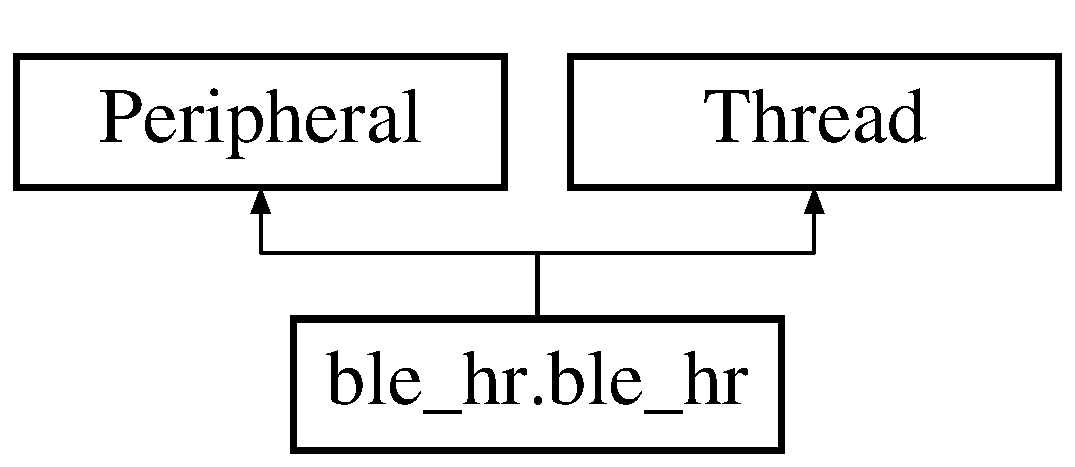
\includegraphics[height=2.000000cm]{classble__hr_1_1ble__hr}
\end{center}
\end{figure}
\subsection*{Public Member Functions}
\begin{DoxyCompactItemize}
\item 
def \hyperlink{classble__hr_1_1ble__hr_af31908249a7579dbdd49df718a789dde}{\+\_\+\+\_\+init\+\_\+\+\_\+} (self, \hyperlink{classble__hr_1_1ble__hr_a57de0d26c0ef685006b704485bc80902}{addr})
\item 
def \hyperlink{classble__hr_1_1ble__hr_a4a5d2a824ad6a9d6d5ed21eaca3e4079}{set\+\_\+notifications} (self, enable=True)
\item 
def \hyperlink{classble__hr_1_1ble__hr_a7d26889af16df11894dacc699d8794fa}{get\+\_\+device\+\_\+name} (self)
\item 
def \hyperlink{classble__hr_1_1ble__hr_aaed07642915896a2ed8cb1c5c6601e9a}{get\+\_\+battery\+\_\+level} (self)
\item 
def \hyperlink{classble__hr_1_1ble__hr_a9d66a38fa21117b6fa70683b8cefeb7d}{get\+\_\+state} (self)
\item 
def \hyperlink{classble__hr_1_1ble__hr_aa64424b260416362b4c248f62092b722}{run} (self)
\item 
def \hyperlink{classble__hr_1_1ble__hr_a95ed9d67bcd7143ec6b6fd52c03d98dc}{get\+\_\+data} (self)
\item 
def \hyperlink{classble__hr_1_1ble__hr_a3fa494427d7fd43856c5e31d37535827}{\+\_\+\+\_\+del\+\_\+\+\_\+} (self)
\item 
def \hyperlink{classble__hr_1_1ble__hr_a68b20bb308e103a3b9a2249d80c17c8b}{stop} (self)
\end{DoxyCompactItemize}
\subsection*{Public Attributes}
\begin{DoxyCompactItemize}
\item 
\hyperlink{classble__hr_1_1ble__hr_a82fd3d4aeb109601084a6e18b9edcae1}{l}
\item 
\hyperlink{classble__hr_1_1ble__hr_a16c7c73e0e680ed4e75d2bb3ce3c8be6}{connected}
\item 
\hyperlink{classble__hr_1_1ble__hr_af6078f5d64042eb96472a6cd58c628c7}{state}
\item 
\hyperlink{classble__hr_1_1ble__hr_ad10bbee4f4ec4c0b14bb18cd41f16f5a}{heart\+\_\+rate}
\item 
\hyperlink{classble__hr_1_1ble__hr_a84c65caf99b9c4581310c20440a2f79d}{time\+\_\+stamp}
\item 
\hyperlink{classble__hr_1_1ble__hr_a57de0d26c0ef685006b704485bc80902}{addr}
\item 
\hyperlink{classble__hr_1_1ble__hr_ad066520110396ab007fdede6fa964f09}{name}
\item 
\hyperlink{classble__hr_1_1ble__hr_af7f3d4a78f3f741ca4228e51bb99bc19}{delegate}
\end{DoxyCompactItemize}
\subsection*{Static Public Attributes}
\begin{DoxyCompactItemize}
\item 
int \hyperlink{classble__hr_1_1ble__hr_a574a704352ba524a64a2848b007fea0e}{H\+R\+\_\+\+H\+A\+N\+D\+LE} = 0x000f
\item 
string \hyperlink{classble__hr_1_1ble__hr_a0c7c049dc28ba565716bad3f7c39440b}{H\+R\+\_\+\+E\+N\+A\+B\+L\+E\+\_\+\+HR} = \char`\"{}10\char`\"{}
\item 
int \hyperlink{classble__hr_1_1ble__hr_ac59cab95f8364859fc1de4eb30662e27}{W\+A\+I\+T\+\_\+\+T\+I\+ME} = 1
\item 
int \hyperlink{classble__hr_1_1ble__hr_a04d3ee726f59e2de0318d6f2701def7f}{E\+X\+C\+E\+P\+T\+I\+O\+N\+\_\+\+W\+A\+I\+T\+\_\+\+T\+I\+ME} = 10
\end{DoxyCompactItemize}


\subsection{Constructor \& Destructor Documentation}
\mbox{\Hypertarget{classble__hr_1_1ble__hr_af31908249a7579dbdd49df718a789dde}\label{classble__hr_1_1ble__hr_af31908249a7579dbdd49df718a789dde}} 
\index{ble\+\_\+hr\+::ble\+\_\+hr@{ble\+\_\+hr\+::ble\+\_\+hr}!\+\_\+\+\_\+init\+\_\+\+\_\+@{\+\_\+\+\_\+init\+\_\+\+\_\+}}
\index{\+\_\+\+\_\+init\+\_\+\+\_\+@{\+\_\+\+\_\+init\+\_\+\+\_\+}!ble\+\_\+hr\+::ble\+\_\+hr@{ble\+\_\+hr\+::ble\+\_\+hr}}
\subsubsection{\texorpdfstring{\+\_\+\+\_\+init\+\_\+\+\_\+()}{\_\_init\_\_()}}
{\footnotesize\ttfamily def ble\+\_\+hr.\+ble\+\_\+hr.\+\_\+\+\_\+init\+\_\+\+\_\+ (\begin{DoxyParamCaption}\item[{}]{self,  }\item[{}]{addr }\end{DoxyParamCaption})}

\mbox{\Hypertarget{classble__hr_1_1ble__hr_a3fa494427d7fd43856c5e31d37535827}\label{classble__hr_1_1ble__hr_a3fa494427d7fd43856c5e31d37535827}} 
\index{ble\+\_\+hr\+::ble\+\_\+hr@{ble\+\_\+hr\+::ble\+\_\+hr}!\+\_\+\+\_\+del\+\_\+\+\_\+@{\+\_\+\+\_\+del\+\_\+\+\_\+}}
\index{\+\_\+\+\_\+del\+\_\+\+\_\+@{\+\_\+\+\_\+del\+\_\+\+\_\+}!ble\+\_\+hr\+::ble\+\_\+hr@{ble\+\_\+hr\+::ble\+\_\+hr}}
\subsubsection{\texorpdfstring{\+\_\+\+\_\+del\+\_\+\+\_\+()}{\_\_del\_\_()}}
{\footnotesize\ttfamily def ble\+\_\+hr.\+ble\+\_\+hr.\+\_\+\+\_\+del\+\_\+\+\_\+ (\begin{DoxyParamCaption}\item[{}]{self }\end{DoxyParamCaption})}



\subsection{Member Function Documentation}
\mbox{\Hypertarget{classble__hr_1_1ble__hr_aaed07642915896a2ed8cb1c5c6601e9a}\label{classble__hr_1_1ble__hr_aaed07642915896a2ed8cb1c5c6601e9a}} 
\index{ble\+\_\+hr\+::ble\+\_\+hr@{ble\+\_\+hr\+::ble\+\_\+hr}!get\+\_\+battery\+\_\+level@{get\+\_\+battery\+\_\+level}}
\index{get\+\_\+battery\+\_\+level@{get\+\_\+battery\+\_\+level}!ble\+\_\+hr\+::ble\+\_\+hr@{ble\+\_\+hr\+::ble\+\_\+hr}}
\subsubsection{\texorpdfstring{get\+\_\+battery\+\_\+level()}{get\_battery\_level()}}
{\footnotesize\ttfamily def ble\+\_\+hr.\+ble\+\_\+hr.\+get\+\_\+battery\+\_\+level (\begin{DoxyParamCaption}\item[{}]{self }\end{DoxyParamCaption})}

\mbox{\Hypertarget{classble__hr_1_1ble__hr_a95ed9d67bcd7143ec6b6fd52c03d98dc}\label{classble__hr_1_1ble__hr_a95ed9d67bcd7143ec6b6fd52c03d98dc}} 
\index{ble\+\_\+hr\+::ble\+\_\+hr@{ble\+\_\+hr\+::ble\+\_\+hr}!get\+\_\+data@{get\+\_\+data}}
\index{get\+\_\+data@{get\+\_\+data}!ble\+\_\+hr\+::ble\+\_\+hr@{ble\+\_\+hr\+::ble\+\_\+hr}}
\subsubsection{\texorpdfstring{get\+\_\+data()}{get\_data()}}
{\footnotesize\ttfamily def ble\+\_\+hr.\+ble\+\_\+hr.\+get\+\_\+data (\begin{DoxyParamCaption}\item[{}]{self }\end{DoxyParamCaption})}

\mbox{\Hypertarget{classble__hr_1_1ble__hr_a7d26889af16df11894dacc699d8794fa}\label{classble__hr_1_1ble__hr_a7d26889af16df11894dacc699d8794fa}} 
\index{ble\+\_\+hr\+::ble\+\_\+hr@{ble\+\_\+hr\+::ble\+\_\+hr}!get\+\_\+device\+\_\+name@{get\+\_\+device\+\_\+name}}
\index{get\+\_\+device\+\_\+name@{get\+\_\+device\+\_\+name}!ble\+\_\+hr\+::ble\+\_\+hr@{ble\+\_\+hr\+::ble\+\_\+hr}}
\subsubsection{\texorpdfstring{get\+\_\+device\+\_\+name()}{get\_device\_name()}}
{\footnotesize\ttfamily def ble\+\_\+hr.\+ble\+\_\+hr.\+get\+\_\+device\+\_\+name (\begin{DoxyParamCaption}\item[{}]{self }\end{DoxyParamCaption})}

\mbox{\Hypertarget{classble__hr_1_1ble__hr_a9d66a38fa21117b6fa70683b8cefeb7d}\label{classble__hr_1_1ble__hr_a9d66a38fa21117b6fa70683b8cefeb7d}} 
\index{ble\+\_\+hr\+::ble\+\_\+hr@{ble\+\_\+hr\+::ble\+\_\+hr}!get\+\_\+state@{get\+\_\+state}}
\index{get\+\_\+state@{get\+\_\+state}!ble\+\_\+hr\+::ble\+\_\+hr@{ble\+\_\+hr\+::ble\+\_\+hr}}
\subsubsection{\texorpdfstring{get\+\_\+state()}{get\_state()}}
{\footnotesize\ttfamily def ble\+\_\+hr.\+ble\+\_\+hr.\+get\+\_\+state (\begin{DoxyParamCaption}\item[{}]{self }\end{DoxyParamCaption})}

\mbox{\Hypertarget{classble__hr_1_1ble__hr_aa64424b260416362b4c248f62092b722}\label{classble__hr_1_1ble__hr_aa64424b260416362b4c248f62092b722}} 
\index{ble\+\_\+hr\+::ble\+\_\+hr@{ble\+\_\+hr\+::ble\+\_\+hr}!run@{run}}
\index{run@{run}!ble\+\_\+hr\+::ble\+\_\+hr@{ble\+\_\+hr\+::ble\+\_\+hr}}
\subsubsection{\texorpdfstring{run()}{run()}}
{\footnotesize\ttfamily def ble\+\_\+hr.\+ble\+\_\+hr.\+run (\begin{DoxyParamCaption}\item[{}]{self }\end{DoxyParamCaption})}

\mbox{\Hypertarget{classble__hr_1_1ble__hr_a4a5d2a824ad6a9d6d5ed21eaca3e4079}\label{classble__hr_1_1ble__hr_a4a5d2a824ad6a9d6d5ed21eaca3e4079}} 
\index{ble\+\_\+hr\+::ble\+\_\+hr@{ble\+\_\+hr\+::ble\+\_\+hr}!set\+\_\+notifications@{set\+\_\+notifications}}
\index{set\+\_\+notifications@{set\+\_\+notifications}!ble\+\_\+hr\+::ble\+\_\+hr@{ble\+\_\+hr\+::ble\+\_\+hr}}
\subsubsection{\texorpdfstring{set\+\_\+notifications()}{set\_notifications()}}
{\footnotesize\ttfamily def ble\+\_\+hr.\+ble\+\_\+hr.\+set\+\_\+notifications (\begin{DoxyParamCaption}\item[{}]{self,  }\item[{}]{enable = {\ttfamily True} }\end{DoxyParamCaption})}

\mbox{\Hypertarget{classble__hr_1_1ble__hr_a68b20bb308e103a3b9a2249d80c17c8b}\label{classble__hr_1_1ble__hr_a68b20bb308e103a3b9a2249d80c17c8b}} 
\index{ble\+\_\+hr\+::ble\+\_\+hr@{ble\+\_\+hr\+::ble\+\_\+hr}!stop@{stop}}
\index{stop@{stop}!ble\+\_\+hr\+::ble\+\_\+hr@{ble\+\_\+hr\+::ble\+\_\+hr}}
\subsubsection{\texorpdfstring{stop()}{stop()}}
{\footnotesize\ttfamily def ble\+\_\+hr.\+ble\+\_\+hr.\+stop (\begin{DoxyParamCaption}\item[{}]{self }\end{DoxyParamCaption})}



\subsection{Member Data Documentation}
\mbox{\Hypertarget{classble__hr_1_1ble__hr_a57de0d26c0ef685006b704485bc80902}\label{classble__hr_1_1ble__hr_a57de0d26c0ef685006b704485bc80902}} 
\index{ble\+\_\+hr\+::ble\+\_\+hr@{ble\+\_\+hr\+::ble\+\_\+hr}!addr@{addr}}
\index{addr@{addr}!ble\+\_\+hr\+::ble\+\_\+hr@{ble\+\_\+hr\+::ble\+\_\+hr}}
\subsubsection{\texorpdfstring{addr}{addr}}
{\footnotesize\ttfamily ble\+\_\+hr.\+ble\+\_\+hr.\+addr}

\mbox{\Hypertarget{classble__hr_1_1ble__hr_a16c7c73e0e680ed4e75d2bb3ce3c8be6}\label{classble__hr_1_1ble__hr_a16c7c73e0e680ed4e75d2bb3ce3c8be6}} 
\index{ble\+\_\+hr\+::ble\+\_\+hr@{ble\+\_\+hr\+::ble\+\_\+hr}!connected@{connected}}
\index{connected@{connected}!ble\+\_\+hr\+::ble\+\_\+hr@{ble\+\_\+hr\+::ble\+\_\+hr}}
\subsubsection{\texorpdfstring{connected}{connected}}
{\footnotesize\ttfamily ble\+\_\+hr.\+ble\+\_\+hr.\+connected}

\mbox{\Hypertarget{classble__hr_1_1ble__hr_af7f3d4a78f3f741ca4228e51bb99bc19}\label{classble__hr_1_1ble__hr_af7f3d4a78f3f741ca4228e51bb99bc19}} 
\index{ble\+\_\+hr\+::ble\+\_\+hr@{ble\+\_\+hr\+::ble\+\_\+hr}!delegate@{delegate}}
\index{delegate@{delegate}!ble\+\_\+hr\+::ble\+\_\+hr@{ble\+\_\+hr\+::ble\+\_\+hr}}
\subsubsection{\texorpdfstring{delegate}{delegate}}
{\footnotesize\ttfamily ble\+\_\+hr.\+ble\+\_\+hr.\+delegate}

\mbox{\Hypertarget{classble__hr_1_1ble__hr_a04d3ee726f59e2de0318d6f2701def7f}\label{classble__hr_1_1ble__hr_a04d3ee726f59e2de0318d6f2701def7f}} 
\index{ble\+\_\+hr\+::ble\+\_\+hr@{ble\+\_\+hr\+::ble\+\_\+hr}!E\+X\+C\+E\+P\+T\+I\+O\+N\+\_\+\+W\+A\+I\+T\+\_\+\+T\+I\+ME@{E\+X\+C\+E\+P\+T\+I\+O\+N\+\_\+\+W\+A\+I\+T\+\_\+\+T\+I\+ME}}
\index{E\+X\+C\+E\+P\+T\+I\+O\+N\+\_\+\+W\+A\+I\+T\+\_\+\+T\+I\+ME@{E\+X\+C\+E\+P\+T\+I\+O\+N\+\_\+\+W\+A\+I\+T\+\_\+\+T\+I\+ME}!ble\+\_\+hr\+::ble\+\_\+hr@{ble\+\_\+hr\+::ble\+\_\+hr}}
\subsubsection{\texorpdfstring{E\+X\+C\+E\+P\+T\+I\+O\+N\+\_\+\+W\+A\+I\+T\+\_\+\+T\+I\+ME}{EXCEPTION\_WAIT\_TIME}}
{\footnotesize\ttfamily int ble\+\_\+hr.\+ble\+\_\+hr.\+E\+X\+C\+E\+P\+T\+I\+O\+N\+\_\+\+W\+A\+I\+T\+\_\+\+T\+I\+ME = 10\hspace{0.3cm}{\ttfamily [static]}}

\mbox{\Hypertarget{classble__hr_1_1ble__hr_ad10bbee4f4ec4c0b14bb18cd41f16f5a}\label{classble__hr_1_1ble__hr_ad10bbee4f4ec4c0b14bb18cd41f16f5a}} 
\index{ble\+\_\+hr\+::ble\+\_\+hr@{ble\+\_\+hr\+::ble\+\_\+hr}!heart\+\_\+rate@{heart\+\_\+rate}}
\index{heart\+\_\+rate@{heart\+\_\+rate}!ble\+\_\+hr\+::ble\+\_\+hr@{ble\+\_\+hr\+::ble\+\_\+hr}}
\subsubsection{\texorpdfstring{heart\+\_\+rate}{heart\_rate}}
{\footnotesize\ttfamily ble\+\_\+hr.\+ble\+\_\+hr.\+heart\+\_\+rate}

\mbox{\Hypertarget{classble__hr_1_1ble__hr_a0c7c049dc28ba565716bad3f7c39440b}\label{classble__hr_1_1ble__hr_a0c7c049dc28ba565716bad3f7c39440b}} 
\index{ble\+\_\+hr\+::ble\+\_\+hr@{ble\+\_\+hr\+::ble\+\_\+hr}!H\+R\+\_\+\+E\+N\+A\+B\+L\+E\+\_\+\+HR@{H\+R\+\_\+\+E\+N\+A\+B\+L\+E\+\_\+\+HR}}
\index{H\+R\+\_\+\+E\+N\+A\+B\+L\+E\+\_\+\+HR@{H\+R\+\_\+\+E\+N\+A\+B\+L\+E\+\_\+\+HR}!ble\+\_\+hr\+::ble\+\_\+hr@{ble\+\_\+hr\+::ble\+\_\+hr}}
\subsubsection{\texorpdfstring{H\+R\+\_\+\+E\+N\+A\+B\+L\+E\+\_\+\+HR}{HR\_ENABLE\_HR}}
{\footnotesize\ttfamily string ble\+\_\+hr.\+ble\+\_\+hr.\+H\+R\+\_\+\+E\+N\+A\+B\+L\+E\+\_\+\+HR = \char`\"{}10\char`\"{}\hspace{0.3cm}{\ttfamily [static]}}

\mbox{\Hypertarget{classble__hr_1_1ble__hr_a574a704352ba524a64a2848b007fea0e}\label{classble__hr_1_1ble__hr_a574a704352ba524a64a2848b007fea0e}} 
\index{ble\+\_\+hr\+::ble\+\_\+hr@{ble\+\_\+hr\+::ble\+\_\+hr}!H\+R\+\_\+\+H\+A\+N\+D\+LE@{H\+R\+\_\+\+H\+A\+N\+D\+LE}}
\index{H\+R\+\_\+\+H\+A\+N\+D\+LE@{H\+R\+\_\+\+H\+A\+N\+D\+LE}!ble\+\_\+hr\+::ble\+\_\+hr@{ble\+\_\+hr\+::ble\+\_\+hr}}
\subsubsection{\texorpdfstring{H\+R\+\_\+\+H\+A\+N\+D\+LE}{HR\_HANDLE}}
{\footnotesize\ttfamily int ble\+\_\+hr.\+ble\+\_\+hr.\+H\+R\+\_\+\+H\+A\+N\+D\+LE = 0x000f\hspace{0.3cm}{\ttfamily [static]}}

\mbox{\Hypertarget{classble__hr_1_1ble__hr_a82fd3d4aeb109601084a6e18b9edcae1}\label{classble__hr_1_1ble__hr_a82fd3d4aeb109601084a6e18b9edcae1}} 
\index{ble\+\_\+hr\+::ble\+\_\+hr@{ble\+\_\+hr\+::ble\+\_\+hr}!l@{l}}
\index{l@{l}!ble\+\_\+hr\+::ble\+\_\+hr@{ble\+\_\+hr\+::ble\+\_\+hr}}
\subsubsection{\texorpdfstring{l}{l}}
{\footnotesize\ttfamily ble\+\_\+hr.\+ble\+\_\+hr.\+l}

\mbox{\Hypertarget{classble__hr_1_1ble__hr_ad066520110396ab007fdede6fa964f09}\label{classble__hr_1_1ble__hr_ad066520110396ab007fdede6fa964f09}} 
\index{ble\+\_\+hr\+::ble\+\_\+hr@{ble\+\_\+hr\+::ble\+\_\+hr}!name@{name}}
\index{name@{name}!ble\+\_\+hr\+::ble\+\_\+hr@{ble\+\_\+hr\+::ble\+\_\+hr}}
\subsubsection{\texorpdfstring{name}{name}}
{\footnotesize\ttfamily ble\+\_\+hr.\+ble\+\_\+hr.\+name}

\mbox{\Hypertarget{classble__hr_1_1ble__hr_af6078f5d64042eb96472a6cd58c628c7}\label{classble__hr_1_1ble__hr_af6078f5d64042eb96472a6cd58c628c7}} 
\index{ble\+\_\+hr\+::ble\+\_\+hr@{ble\+\_\+hr\+::ble\+\_\+hr}!state@{state}}
\index{state@{state}!ble\+\_\+hr\+::ble\+\_\+hr@{ble\+\_\+hr\+::ble\+\_\+hr}}
\subsubsection{\texorpdfstring{state}{state}}
{\footnotesize\ttfamily ble\+\_\+hr.\+ble\+\_\+hr.\+state}

\mbox{\Hypertarget{classble__hr_1_1ble__hr_a84c65caf99b9c4581310c20440a2f79d}\label{classble__hr_1_1ble__hr_a84c65caf99b9c4581310c20440a2f79d}} 
\index{ble\+\_\+hr\+::ble\+\_\+hr@{ble\+\_\+hr\+::ble\+\_\+hr}!time\+\_\+stamp@{time\+\_\+stamp}}
\index{time\+\_\+stamp@{time\+\_\+stamp}!ble\+\_\+hr\+::ble\+\_\+hr@{ble\+\_\+hr\+::ble\+\_\+hr}}
\subsubsection{\texorpdfstring{time\+\_\+stamp}{time\_stamp}}
{\footnotesize\ttfamily ble\+\_\+hr.\+ble\+\_\+hr.\+time\+\_\+stamp}

\mbox{\Hypertarget{classble__hr_1_1ble__hr_ac59cab95f8364859fc1de4eb30662e27}\label{classble__hr_1_1ble__hr_ac59cab95f8364859fc1de4eb30662e27}} 
\index{ble\+\_\+hr\+::ble\+\_\+hr@{ble\+\_\+hr\+::ble\+\_\+hr}!W\+A\+I\+T\+\_\+\+T\+I\+ME@{W\+A\+I\+T\+\_\+\+T\+I\+ME}}
\index{W\+A\+I\+T\+\_\+\+T\+I\+ME@{W\+A\+I\+T\+\_\+\+T\+I\+ME}!ble\+\_\+hr\+::ble\+\_\+hr@{ble\+\_\+hr\+::ble\+\_\+hr}}
\subsubsection{\texorpdfstring{W\+A\+I\+T\+\_\+\+T\+I\+ME}{WAIT\_TIME}}
{\footnotesize\ttfamily int ble\+\_\+hr.\+ble\+\_\+hr.\+W\+A\+I\+T\+\_\+\+T\+I\+ME = 1\hspace{0.3cm}{\ttfamily [static]}}



The documentation for this class was generated from the following file\+:\begin{DoxyCompactItemize}
\item 
src/\hyperlink{ble__hr_8py}{ble\+\_\+hr.\+py}\end{DoxyCompactItemize}

\hypertarget{classble__sc_1_1ble__sc}{}\section{ble\+\_\+sc.\+ble\+\_\+sc Class Reference}
\label{classble__sc_1_1ble__sc}\index{ble\+\_\+sc.\+ble\+\_\+sc@{ble\+\_\+sc.\+ble\+\_\+sc}}
Inheritance diagram for ble\+\_\+sc.\+ble\+\_\+sc\+:\begin{figure}[H]
\begin{center}
\leavevmode
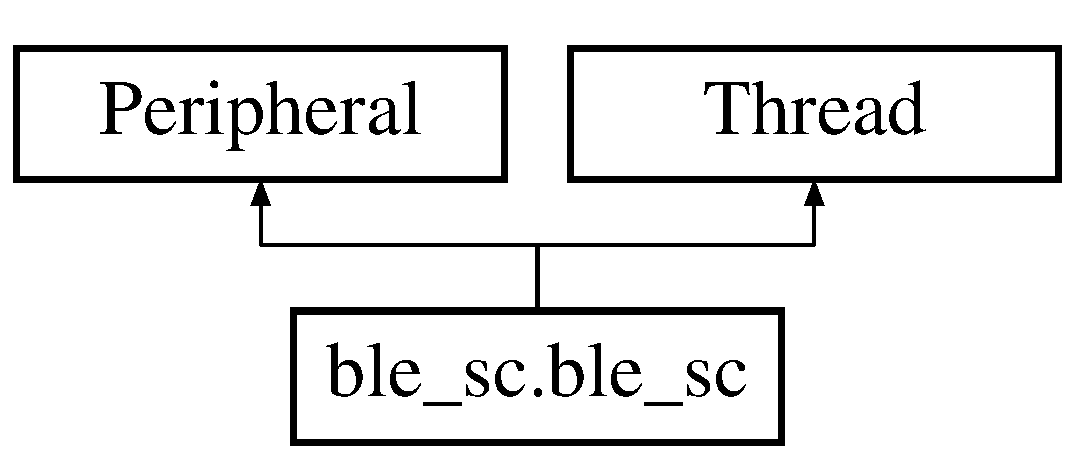
\includegraphics[height=2.000000cm]{classble__sc_1_1ble__sc}
\end{center}
\end{figure}
\subsection*{Public Member Functions}
\begin{DoxyCompactItemize}
\item 
def \hyperlink{classble__sc_1_1ble__sc_aa2c805418fadd328a3fda4c08cd267e9}{\+\_\+\+\_\+init\+\_\+\+\_\+} (self, \hyperlink{classble__sc_1_1ble__sc_afa92ff7157c4bdf0af9755643135f930}{addr})
\item 
def \hyperlink{classble__sc_1_1ble__sc_a1de425ebd84b004a47b68be4707f0c81}{set\+\_\+notifications} (self, enable=True)
\item 
def \hyperlink{classble__sc_1_1ble__sc_abe9b03263bd0d7e8db523e940b13794a}{get\+\_\+device\+\_\+name} (self)
\item 
def \hyperlink{classble__sc_1_1ble__sc_a20b6268e202b79883c487ca3826fe521}{get\+\_\+battery\+\_\+level} (self)
\item 
def \hyperlink{classble__sc_1_1ble__sc_a412188403c86a115b1457c731c3b8b03}{get\+\_\+state} (self)
\item 
def \hyperlink{classble__sc_1_1ble__sc_ad54a981de790eff2f9543fd28c1d21fb}{run} (self)
\item 
def \hyperlink{classble__sc_1_1ble__sc_a97ac48791074b904c8fa68c9ce0f709f}{get\+\_\+data} (self)
\item 
def \hyperlink{classble__sc_1_1ble__sc_a8df772741eddf5d86cabcf98587e7439}{\+\_\+\+\_\+del\+\_\+\+\_\+} (self)
\item 
def \hyperlink{classble__sc_1_1ble__sc_ae3ccbb4eed28452868695db039c1d9d2}{stop} (self)
\end{DoxyCompactItemize}
\subsection*{Public Attributes}
\begin{DoxyCompactItemize}
\item 
\hyperlink{classble__sc_1_1ble__sc_abb5cd42cfd059b02e9bbde16ca692aca}{l}
\item 
\hyperlink{classble__sc_1_1ble__sc_a7febc900c7ebe07ef23edea4bf736b6d}{connected}
\item 
\hyperlink{classble__sc_1_1ble__sc_af56b72b355ef5e792a0287ebffce36ff}{state}
\item 
\hyperlink{classble__sc_1_1ble__sc_afa92ff7157c4bdf0af9755643135f930}{addr}
\item 
\hyperlink{classble__sc_1_1ble__sc_ad24e9283f4f1dea4a26d8ce1ad1035ce}{wheel\+\_\+time\+\_\+stamp}
\item 
\hyperlink{classble__sc_1_1ble__sc_adb16b829976874cd3e8908f550d60b6d}{wheel\+\_\+rev\+\_\+time}
\item 
\hyperlink{classble__sc_1_1ble__sc_ae56d6dc864f7514593ada1a67d3bba0f}{cadence\+\_\+time\+\_\+stamp}
\item 
\hyperlink{classble__sc_1_1ble__sc_a9f5a63641420b643213f0559edb2790f}{cadence}
\item 
\hyperlink{classble__sc_1_1ble__sc_a771332ac7fe0fd02cf9c0373f993f785}{name}
\item 
\hyperlink{classble__sc_1_1ble__sc_a01f09adb9eaf400be64de2a8a0ec3044}{delegate}
\end{DoxyCompactItemize}
\subsection*{Static Public Attributes}
\begin{DoxyCompactItemize}
\item 
int \hyperlink{classble__sc_1_1ble__sc_a67d10b5658a576b2e50667fc3741b0dc}{C\+S\+C\+\_\+\+H\+A\+N\+D\+LE} = 0x000f
\item 
string \hyperlink{classble__sc_1_1ble__sc_a6b2fe95bf3346e236e96efd5fdfafd5c}{C\+S\+C\+\_\+\+E\+N\+A\+B\+L\+E\+\_\+\+SC} = \char`\"{}10\char`\"{}
\item 
float \hyperlink{classble__sc_1_1ble__sc_a7c1e25208c6e93d5bd9fd4f8eafc4833}{W\+A\+I\+T\+\_\+\+T\+I\+ME} = 0.\+3
\item 
int \hyperlink{classble__sc_1_1ble__sc_a0c45928e56f439c14eab8356c16cc6cc}{E\+X\+C\+E\+P\+T\+I\+O\+N\+\_\+\+W\+A\+I\+T\+\_\+\+T\+I\+ME} = 10
\end{DoxyCompactItemize}


\subsection{Constructor \& Destructor Documentation}
\mbox{\Hypertarget{classble__sc_1_1ble__sc_aa2c805418fadd328a3fda4c08cd267e9}\label{classble__sc_1_1ble__sc_aa2c805418fadd328a3fda4c08cd267e9}} 
\index{ble\+\_\+sc\+::ble\+\_\+sc@{ble\+\_\+sc\+::ble\+\_\+sc}!\+\_\+\+\_\+init\+\_\+\+\_\+@{\+\_\+\+\_\+init\+\_\+\+\_\+}}
\index{\+\_\+\+\_\+init\+\_\+\+\_\+@{\+\_\+\+\_\+init\+\_\+\+\_\+}!ble\+\_\+sc\+::ble\+\_\+sc@{ble\+\_\+sc\+::ble\+\_\+sc}}
\subsubsection{\texorpdfstring{\+\_\+\+\_\+init\+\_\+\+\_\+()}{\_\_init\_\_()}}
{\footnotesize\ttfamily def ble\+\_\+sc.\+ble\+\_\+sc.\+\_\+\+\_\+init\+\_\+\+\_\+ (\begin{DoxyParamCaption}\item[{}]{self,  }\item[{}]{addr }\end{DoxyParamCaption})}

\mbox{\Hypertarget{classble__sc_1_1ble__sc_a8df772741eddf5d86cabcf98587e7439}\label{classble__sc_1_1ble__sc_a8df772741eddf5d86cabcf98587e7439}} 
\index{ble\+\_\+sc\+::ble\+\_\+sc@{ble\+\_\+sc\+::ble\+\_\+sc}!\+\_\+\+\_\+del\+\_\+\+\_\+@{\+\_\+\+\_\+del\+\_\+\+\_\+}}
\index{\+\_\+\+\_\+del\+\_\+\+\_\+@{\+\_\+\+\_\+del\+\_\+\+\_\+}!ble\+\_\+sc\+::ble\+\_\+sc@{ble\+\_\+sc\+::ble\+\_\+sc}}
\subsubsection{\texorpdfstring{\+\_\+\+\_\+del\+\_\+\+\_\+()}{\_\_del\_\_()}}
{\footnotesize\ttfamily def ble\+\_\+sc.\+ble\+\_\+sc.\+\_\+\+\_\+del\+\_\+\+\_\+ (\begin{DoxyParamCaption}\item[{}]{self }\end{DoxyParamCaption})}



\subsection{Member Function Documentation}
\mbox{\Hypertarget{classble__sc_1_1ble__sc_a20b6268e202b79883c487ca3826fe521}\label{classble__sc_1_1ble__sc_a20b6268e202b79883c487ca3826fe521}} 
\index{ble\+\_\+sc\+::ble\+\_\+sc@{ble\+\_\+sc\+::ble\+\_\+sc}!get\+\_\+battery\+\_\+level@{get\+\_\+battery\+\_\+level}}
\index{get\+\_\+battery\+\_\+level@{get\+\_\+battery\+\_\+level}!ble\+\_\+sc\+::ble\+\_\+sc@{ble\+\_\+sc\+::ble\+\_\+sc}}
\subsubsection{\texorpdfstring{get\+\_\+battery\+\_\+level()}{get\_battery\_level()}}
{\footnotesize\ttfamily def ble\+\_\+sc.\+ble\+\_\+sc.\+get\+\_\+battery\+\_\+level (\begin{DoxyParamCaption}\item[{}]{self }\end{DoxyParamCaption})}

\mbox{\Hypertarget{classble__sc_1_1ble__sc_a97ac48791074b904c8fa68c9ce0f709f}\label{classble__sc_1_1ble__sc_a97ac48791074b904c8fa68c9ce0f709f}} 
\index{ble\+\_\+sc\+::ble\+\_\+sc@{ble\+\_\+sc\+::ble\+\_\+sc}!get\+\_\+data@{get\+\_\+data}}
\index{get\+\_\+data@{get\+\_\+data}!ble\+\_\+sc\+::ble\+\_\+sc@{ble\+\_\+sc\+::ble\+\_\+sc}}
\subsubsection{\texorpdfstring{get\+\_\+data()}{get\_data()}}
{\footnotesize\ttfamily def ble\+\_\+sc.\+ble\+\_\+sc.\+get\+\_\+data (\begin{DoxyParamCaption}\item[{}]{self }\end{DoxyParamCaption})}

\mbox{\Hypertarget{classble__sc_1_1ble__sc_abe9b03263bd0d7e8db523e940b13794a}\label{classble__sc_1_1ble__sc_abe9b03263bd0d7e8db523e940b13794a}} 
\index{ble\+\_\+sc\+::ble\+\_\+sc@{ble\+\_\+sc\+::ble\+\_\+sc}!get\+\_\+device\+\_\+name@{get\+\_\+device\+\_\+name}}
\index{get\+\_\+device\+\_\+name@{get\+\_\+device\+\_\+name}!ble\+\_\+sc\+::ble\+\_\+sc@{ble\+\_\+sc\+::ble\+\_\+sc}}
\subsubsection{\texorpdfstring{get\+\_\+device\+\_\+name()}{get\_device\_name()}}
{\footnotesize\ttfamily def ble\+\_\+sc.\+ble\+\_\+sc.\+get\+\_\+device\+\_\+name (\begin{DoxyParamCaption}\item[{}]{self }\end{DoxyParamCaption})}

\mbox{\Hypertarget{classble__sc_1_1ble__sc_a412188403c86a115b1457c731c3b8b03}\label{classble__sc_1_1ble__sc_a412188403c86a115b1457c731c3b8b03}} 
\index{ble\+\_\+sc\+::ble\+\_\+sc@{ble\+\_\+sc\+::ble\+\_\+sc}!get\+\_\+state@{get\+\_\+state}}
\index{get\+\_\+state@{get\+\_\+state}!ble\+\_\+sc\+::ble\+\_\+sc@{ble\+\_\+sc\+::ble\+\_\+sc}}
\subsubsection{\texorpdfstring{get\+\_\+state()}{get\_state()}}
{\footnotesize\ttfamily def ble\+\_\+sc.\+ble\+\_\+sc.\+get\+\_\+state (\begin{DoxyParamCaption}\item[{}]{self }\end{DoxyParamCaption})}

\mbox{\Hypertarget{classble__sc_1_1ble__sc_ad54a981de790eff2f9543fd28c1d21fb}\label{classble__sc_1_1ble__sc_ad54a981de790eff2f9543fd28c1d21fb}} 
\index{ble\+\_\+sc\+::ble\+\_\+sc@{ble\+\_\+sc\+::ble\+\_\+sc}!run@{run}}
\index{run@{run}!ble\+\_\+sc\+::ble\+\_\+sc@{ble\+\_\+sc\+::ble\+\_\+sc}}
\subsubsection{\texorpdfstring{run()}{run()}}
{\footnotesize\ttfamily def ble\+\_\+sc.\+ble\+\_\+sc.\+run (\begin{DoxyParamCaption}\item[{}]{self }\end{DoxyParamCaption})}

\mbox{\Hypertarget{classble__sc_1_1ble__sc_a1de425ebd84b004a47b68be4707f0c81}\label{classble__sc_1_1ble__sc_a1de425ebd84b004a47b68be4707f0c81}} 
\index{ble\+\_\+sc\+::ble\+\_\+sc@{ble\+\_\+sc\+::ble\+\_\+sc}!set\+\_\+notifications@{set\+\_\+notifications}}
\index{set\+\_\+notifications@{set\+\_\+notifications}!ble\+\_\+sc\+::ble\+\_\+sc@{ble\+\_\+sc\+::ble\+\_\+sc}}
\subsubsection{\texorpdfstring{set\+\_\+notifications()}{set\_notifications()}}
{\footnotesize\ttfamily def ble\+\_\+sc.\+ble\+\_\+sc.\+set\+\_\+notifications (\begin{DoxyParamCaption}\item[{}]{self,  }\item[{}]{enable = {\ttfamily True} }\end{DoxyParamCaption})}

\mbox{\Hypertarget{classble__sc_1_1ble__sc_ae3ccbb4eed28452868695db039c1d9d2}\label{classble__sc_1_1ble__sc_ae3ccbb4eed28452868695db039c1d9d2}} 
\index{ble\+\_\+sc\+::ble\+\_\+sc@{ble\+\_\+sc\+::ble\+\_\+sc}!stop@{stop}}
\index{stop@{stop}!ble\+\_\+sc\+::ble\+\_\+sc@{ble\+\_\+sc\+::ble\+\_\+sc}}
\subsubsection{\texorpdfstring{stop()}{stop()}}
{\footnotesize\ttfamily def ble\+\_\+sc.\+ble\+\_\+sc.\+stop (\begin{DoxyParamCaption}\item[{}]{self }\end{DoxyParamCaption})}



\subsection{Member Data Documentation}
\mbox{\Hypertarget{classble__sc_1_1ble__sc_afa92ff7157c4bdf0af9755643135f930}\label{classble__sc_1_1ble__sc_afa92ff7157c4bdf0af9755643135f930}} 
\index{ble\+\_\+sc\+::ble\+\_\+sc@{ble\+\_\+sc\+::ble\+\_\+sc}!addr@{addr}}
\index{addr@{addr}!ble\+\_\+sc\+::ble\+\_\+sc@{ble\+\_\+sc\+::ble\+\_\+sc}}
\subsubsection{\texorpdfstring{addr}{addr}}
{\footnotesize\ttfamily ble\+\_\+sc.\+ble\+\_\+sc.\+addr}

\mbox{\Hypertarget{classble__sc_1_1ble__sc_a9f5a63641420b643213f0559edb2790f}\label{classble__sc_1_1ble__sc_a9f5a63641420b643213f0559edb2790f}} 
\index{ble\+\_\+sc\+::ble\+\_\+sc@{ble\+\_\+sc\+::ble\+\_\+sc}!cadence@{cadence}}
\index{cadence@{cadence}!ble\+\_\+sc\+::ble\+\_\+sc@{ble\+\_\+sc\+::ble\+\_\+sc}}
\subsubsection{\texorpdfstring{cadence}{cadence}}
{\footnotesize\ttfamily ble\+\_\+sc.\+ble\+\_\+sc.\+cadence}

\mbox{\Hypertarget{classble__sc_1_1ble__sc_ae56d6dc864f7514593ada1a67d3bba0f}\label{classble__sc_1_1ble__sc_ae56d6dc864f7514593ada1a67d3bba0f}} 
\index{ble\+\_\+sc\+::ble\+\_\+sc@{ble\+\_\+sc\+::ble\+\_\+sc}!cadence\+\_\+time\+\_\+stamp@{cadence\+\_\+time\+\_\+stamp}}
\index{cadence\+\_\+time\+\_\+stamp@{cadence\+\_\+time\+\_\+stamp}!ble\+\_\+sc\+::ble\+\_\+sc@{ble\+\_\+sc\+::ble\+\_\+sc}}
\subsubsection{\texorpdfstring{cadence\+\_\+time\+\_\+stamp}{cadence\_time\_stamp}}
{\footnotesize\ttfamily ble\+\_\+sc.\+ble\+\_\+sc.\+cadence\+\_\+time\+\_\+stamp}

\mbox{\Hypertarget{classble__sc_1_1ble__sc_a7febc900c7ebe07ef23edea4bf736b6d}\label{classble__sc_1_1ble__sc_a7febc900c7ebe07ef23edea4bf736b6d}} 
\index{ble\+\_\+sc\+::ble\+\_\+sc@{ble\+\_\+sc\+::ble\+\_\+sc}!connected@{connected}}
\index{connected@{connected}!ble\+\_\+sc\+::ble\+\_\+sc@{ble\+\_\+sc\+::ble\+\_\+sc}}
\subsubsection{\texorpdfstring{connected}{connected}}
{\footnotesize\ttfamily ble\+\_\+sc.\+ble\+\_\+sc.\+connected}

\mbox{\Hypertarget{classble__sc_1_1ble__sc_a6b2fe95bf3346e236e96efd5fdfafd5c}\label{classble__sc_1_1ble__sc_a6b2fe95bf3346e236e96efd5fdfafd5c}} 
\index{ble\+\_\+sc\+::ble\+\_\+sc@{ble\+\_\+sc\+::ble\+\_\+sc}!C\+S\+C\+\_\+\+E\+N\+A\+B\+L\+E\+\_\+\+SC@{C\+S\+C\+\_\+\+E\+N\+A\+B\+L\+E\+\_\+\+SC}}
\index{C\+S\+C\+\_\+\+E\+N\+A\+B\+L\+E\+\_\+\+SC@{C\+S\+C\+\_\+\+E\+N\+A\+B\+L\+E\+\_\+\+SC}!ble\+\_\+sc\+::ble\+\_\+sc@{ble\+\_\+sc\+::ble\+\_\+sc}}
\subsubsection{\texorpdfstring{C\+S\+C\+\_\+\+E\+N\+A\+B\+L\+E\+\_\+\+SC}{CSC\_ENABLE\_SC}}
{\footnotesize\ttfamily string ble\+\_\+sc.\+ble\+\_\+sc.\+C\+S\+C\+\_\+\+E\+N\+A\+B\+L\+E\+\_\+\+SC = \char`\"{}10\char`\"{}\hspace{0.3cm}{\ttfamily [static]}}

\mbox{\Hypertarget{classble__sc_1_1ble__sc_a67d10b5658a576b2e50667fc3741b0dc}\label{classble__sc_1_1ble__sc_a67d10b5658a576b2e50667fc3741b0dc}} 
\index{ble\+\_\+sc\+::ble\+\_\+sc@{ble\+\_\+sc\+::ble\+\_\+sc}!C\+S\+C\+\_\+\+H\+A\+N\+D\+LE@{C\+S\+C\+\_\+\+H\+A\+N\+D\+LE}}
\index{C\+S\+C\+\_\+\+H\+A\+N\+D\+LE@{C\+S\+C\+\_\+\+H\+A\+N\+D\+LE}!ble\+\_\+sc\+::ble\+\_\+sc@{ble\+\_\+sc\+::ble\+\_\+sc}}
\subsubsection{\texorpdfstring{C\+S\+C\+\_\+\+H\+A\+N\+D\+LE}{CSC\_HANDLE}}
{\footnotesize\ttfamily int ble\+\_\+sc.\+ble\+\_\+sc.\+C\+S\+C\+\_\+\+H\+A\+N\+D\+LE = 0x000f\hspace{0.3cm}{\ttfamily [static]}}

\mbox{\Hypertarget{classble__sc_1_1ble__sc_a01f09adb9eaf400be64de2a8a0ec3044}\label{classble__sc_1_1ble__sc_a01f09adb9eaf400be64de2a8a0ec3044}} 
\index{ble\+\_\+sc\+::ble\+\_\+sc@{ble\+\_\+sc\+::ble\+\_\+sc}!delegate@{delegate}}
\index{delegate@{delegate}!ble\+\_\+sc\+::ble\+\_\+sc@{ble\+\_\+sc\+::ble\+\_\+sc}}
\subsubsection{\texorpdfstring{delegate}{delegate}}
{\footnotesize\ttfamily ble\+\_\+sc.\+ble\+\_\+sc.\+delegate}

\mbox{\Hypertarget{classble__sc_1_1ble__sc_a0c45928e56f439c14eab8356c16cc6cc}\label{classble__sc_1_1ble__sc_a0c45928e56f439c14eab8356c16cc6cc}} 
\index{ble\+\_\+sc\+::ble\+\_\+sc@{ble\+\_\+sc\+::ble\+\_\+sc}!E\+X\+C\+E\+P\+T\+I\+O\+N\+\_\+\+W\+A\+I\+T\+\_\+\+T\+I\+ME@{E\+X\+C\+E\+P\+T\+I\+O\+N\+\_\+\+W\+A\+I\+T\+\_\+\+T\+I\+ME}}
\index{E\+X\+C\+E\+P\+T\+I\+O\+N\+\_\+\+W\+A\+I\+T\+\_\+\+T\+I\+ME@{E\+X\+C\+E\+P\+T\+I\+O\+N\+\_\+\+W\+A\+I\+T\+\_\+\+T\+I\+ME}!ble\+\_\+sc\+::ble\+\_\+sc@{ble\+\_\+sc\+::ble\+\_\+sc}}
\subsubsection{\texorpdfstring{E\+X\+C\+E\+P\+T\+I\+O\+N\+\_\+\+W\+A\+I\+T\+\_\+\+T\+I\+ME}{EXCEPTION\_WAIT\_TIME}}
{\footnotesize\ttfamily int ble\+\_\+sc.\+ble\+\_\+sc.\+E\+X\+C\+E\+P\+T\+I\+O\+N\+\_\+\+W\+A\+I\+T\+\_\+\+T\+I\+ME = 10\hspace{0.3cm}{\ttfamily [static]}}

\mbox{\Hypertarget{classble__sc_1_1ble__sc_abb5cd42cfd059b02e9bbde16ca692aca}\label{classble__sc_1_1ble__sc_abb5cd42cfd059b02e9bbde16ca692aca}} 
\index{ble\+\_\+sc\+::ble\+\_\+sc@{ble\+\_\+sc\+::ble\+\_\+sc}!l@{l}}
\index{l@{l}!ble\+\_\+sc\+::ble\+\_\+sc@{ble\+\_\+sc\+::ble\+\_\+sc}}
\subsubsection{\texorpdfstring{l}{l}}
{\footnotesize\ttfamily ble\+\_\+sc.\+ble\+\_\+sc.\+l}

\mbox{\Hypertarget{classble__sc_1_1ble__sc_a771332ac7fe0fd02cf9c0373f993f785}\label{classble__sc_1_1ble__sc_a771332ac7fe0fd02cf9c0373f993f785}} 
\index{ble\+\_\+sc\+::ble\+\_\+sc@{ble\+\_\+sc\+::ble\+\_\+sc}!name@{name}}
\index{name@{name}!ble\+\_\+sc\+::ble\+\_\+sc@{ble\+\_\+sc\+::ble\+\_\+sc}}
\subsubsection{\texorpdfstring{name}{name}}
{\footnotesize\ttfamily ble\+\_\+sc.\+ble\+\_\+sc.\+name}

\mbox{\Hypertarget{classble__sc_1_1ble__sc_af56b72b355ef5e792a0287ebffce36ff}\label{classble__sc_1_1ble__sc_af56b72b355ef5e792a0287ebffce36ff}} 
\index{ble\+\_\+sc\+::ble\+\_\+sc@{ble\+\_\+sc\+::ble\+\_\+sc}!state@{state}}
\index{state@{state}!ble\+\_\+sc\+::ble\+\_\+sc@{ble\+\_\+sc\+::ble\+\_\+sc}}
\subsubsection{\texorpdfstring{state}{state}}
{\footnotesize\ttfamily ble\+\_\+sc.\+ble\+\_\+sc.\+state}

\mbox{\Hypertarget{classble__sc_1_1ble__sc_a7c1e25208c6e93d5bd9fd4f8eafc4833}\label{classble__sc_1_1ble__sc_a7c1e25208c6e93d5bd9fd4f8eafc4833}} 
\index{ble\+\_\+sc\+::ble\+\_\+sc@{ble\+\_\+sc\+::ble\+\_\+sc}!W\+A\+I\+T\+\_\+\+T\+I\+ME@{W\+A\+I\+T\+\_\+\+T\+I\+ME}}
\index{W\+A\+I\+T\+\_\+\+T\+I\+ME@{W\+A\+I\+T\+\_\+\+T\+I\+ME}!ble\+\_\+sc\+::ble\+\_\+sc@{ble\+\_\+sc\+::ble\+\_\+sc}}
\subsubsection{\texorpdfstring{W\+A\+I\+T\+\_\+\+T\+I\+ME}{WAIT\_TIME}}
{\footnotesize\ttfamily float ble\+\_\+sc.\+ble\+\_\+sc.\+W\+A\+I\+T\+\_\+\+T\+I\+ME = 0.\+3\hspace{0.3cm}{\ttfamily [static]}}

\mbox{\Hypertarget{classble__sc_1_1ble__sc_adb16b829976874cd3e8908f550d60b6d}\label{classble__sc_1_1ble__sc_adb16b829976874cd3e8908f550d60b6d}} 
\index{ble\+\_\+sc\+::ble\+\_\+sc@{ble\+\_\+sc\+::ble\+\_\+sc}!wheel\+\_\+rev\+\_\+time@{wheel\+\_\+rev\+\_\+time}}
\index{wheel\+\_\+rev\+\_\+time@{wheel\+\_\+rev\+\_\+time}!ble\+\_\+sc\+::ble\+\_\+sc@{ble\+\_\+sc\+::ble\+\_\+sc}}
\subsubsection{\texorpdfstring{wheel\+\_\+rev\+\_\+time}{wheel\_rev\_time}}
{\footnotesize\ttfamily ble\+\_\+sc.\+ble\+\_\+sc.\+wheel\+\_\+rev\+\_\+time}

\mbox{\Hypertarget{classble__sc_1_1ble__sc_ad24e9283f4f1dea4a26d8ce1ad1035ce}\label{classble__sc_1_1ble__sc_ad24e9283f4f1dea4a26d8ce1ad1035ce}} 
\index{ble\+\_\+sc\+::ble\+\_\+sc@{ble\+\_\+sc\+::ble\+\_\+sc}!wheel\+\_\+time\+\_\+stamp@{wheel\+\_\+time\+\_\+stamp}}
\index{wheel\+\_\+time\+\_\+stamp@{wheel\+\_\+time\+\_\+stamp}!ble\+\_\+sc\+::ble\+\_\+sc@{ble\+\_\+sc\+::ble\+\_\+sc}}
\subsubsection{\texorpdfstring{wheel\+\_\+time\+\_\+stamp}{wheel\_time\_stamp}}
{\footnotesize\ttfamily ble\+\_\+sc.\+ble\+\_\+sc.\+wheel\+\_\+time\+\_\+stamp}



The documentation for this class was generated from the following file\+:\begin{DoxyCompactItemize}
\item 
src/\hyperlink{ble__sc_8py}{ble\+\_\+sc.\+py}\end{DoxyCompactItemize}

\hypertarget{classble__scanner_1_1ble__scan}{}\section{ble\+\_\+scanner.\+ble\+\_\+scan Class Reference}
\label{classble__scanner_1_1ble__scan}\index{ble\+\_\+scanner.\+ble\+\_\+scan@{ble\+\_\+scanner.\+ble\+\_\+scan}}
Inheritance diagram for ble\+\_\+scanner.\+ble\+\_\+scan\+:\begin{figure}[H]
\begin{center}
\leavevmode
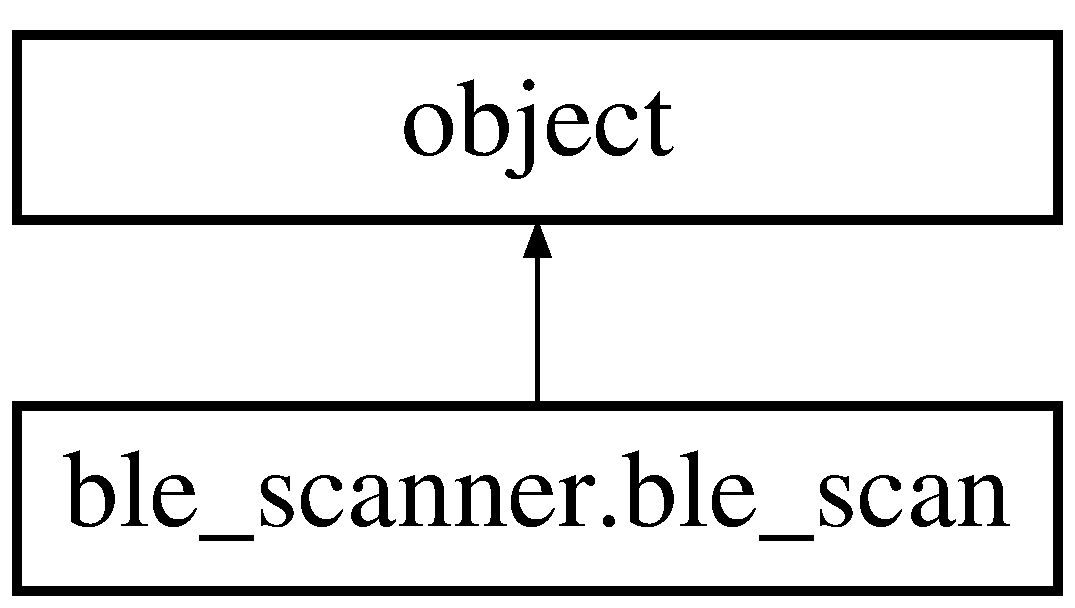
\includegraphics[height=2.000000cm]{classble__scanner_1_1ble__scan}
\end{center}
\end{figure}
\subsection*{Public Member Functions}
\begin{DoxyCompactItemize}
\item 
def \hyperlink{classble__scanner_1_1ble__scan_a4dd1c46e89c06d39bca330a729ac85e2}{\+\_\+\+\_\+init\+\_\+\+\_\+} (self)
\item 
def \hyperlink{classble__scanner_1_1ble__scan_a6cc017eda9dee844afa2837924c2751e}{scan} (self, timeout=10.\+0)
\item 
def \hyperlink{classble__scanner_1_1ble__scan_a9dcebab128bff36843ec70f48401db3c}{get\+\_\+dev\+\_\+list} (self)
\end{DoxyCompactItemize}
\subsection*{Public Attributes}
\begin{DoxyCompactItemize}
\item 
\hyperlink{classble__scanner_1_1ble__scan_a65324c2e86baf31f888af67adff2fa2d}{scanner}
\item 
\hyperlink{classble__scanner_1_1ble__scan_ad0afbee6b99ed29929fcd907117a44b8}{dev\+\_\+list\+\_\+raw}
\end{DoxyCompactItemize}


\subsection{Constructor \& Destructor Documentation}
\mbox{\Hypertarget{classble__scanner_1_1ble__scan_a4dd1c46e89c06d39bca330a729ac85e2}\label{classble__scanner_1_1ble__scan_a4dd1c46e89c06d39bca330a729ac85e2}} 
\index{ble\+\_\+scanner\+::ble\+\_\+scan@{ble\+\_\+scanner\+::ble\+\_\+scan}!\+\_\+\+\_\+init\+\_\+\+\_\+@{\+\_\+\+\_\+init\+\_\+\+\_\+}}
\index{\+\_\+\+\_\+init\+\_\+\+\_\+@{\+\_\+\+\_\+init\+\_\+\+\_\+}!ble\+\_\+scanner\+::ble\+\_\+scan@{ble\+\_\+scanner\+::ble\+\_\+scan}}
\subsubsection{\texorpdfstring{\+\_\+\+\_\+init\+\_\+\+\_\+()}{\_\_init\_\_()}}
{\footnotesize\ttfamily def ble\+\_\+scanner.\+ble\+\_\+scan.\+\_\+\+\_\+init\+\_\+\+\_\+ (\begin{DoxyParamCaption}\item[{}]{self }\end{DoxyParamCaption})}



\subsection{Member Function Documentation}
\mbox{\Hypertarget{classble__scanner_1_1ble__scan_a9dcebab128bff36843ec70f48401db3c}\label{classble__scanner_1_1ble__scan_a9dcebab128bff36843ec70f48401db3c}} 
\index{ble\+\_\+scanner\+::ble\+\_\+scan@{ble\+\_\+scanner\+::ble\+\_\+scan}!get\+\_\+dev\+\_\+list@{get\+\_\+dev\+\_\+list}}
\index{get\+\_\+dev\+\_\+list@{get\+\_\+dev\+\_\+list}!ble\+\_\+scanner\+::ble\+\_\+scan@{ble\+\_\+scanner\+::ble\+\_\+scan}}
\subsubsection{\texorpdfstring{get\+\_\+dev\+\_\+list()}{get\_dev\_list()}}
{\footnotesize\ttfamily def ble\+\_\+scanner.\+ble\+\_\+scan.\+get\+\_\+dev\+\_\+list (\begin{DoxyParamCaption}\item[{}]{self }\end{DoxyParamCaption})}

\mbox{\Hypertarget{classble__scanner_1_1ble__scan_a6cc017eda9dee844afa2837924c2751e}\label{classble__scanner_1_1ble__scan_a6cc017eda9dee844afa2837924c2751e}} 
\index{ble\+\_\+scanner\+::ble\+\_\+scan@{ble\+\_\+scanner\+::ble\+\_\+scan}!scan@{scan}}
\index{scan@{scan}!ble\+\_\+scanner\+::ble\+\_\+scan@{ble\+\_\+scanner\+::ble\+\_\+scan}}
\subsubsection{\texorpdfstring{scan()}{scan()}}
{\footnotesize\ttfamily def ble\+\_\+scanner.\+ble\+\_\+scan.\+scan (\begin{DoxyParamCaption}\item[{}]{self,  }\item[{}]{timeout = {\ttfamily 10.0} }\end{DoxyParamCaption})}



\subsection{Member Data Documentation}
\mbox{\Hypertarget{classble__scanner_1_1ble__scan_ad0afbee6b99ed29929fcd907117a44b8}\label{classble__scanner_1_1ble__scan_ad0afbee6b99ed29929fcd907117a44b8}} 
\index{ble\+\_\+scanner\+::ble\+\_\+scan@{ble\+\_\+scanner\+::ble\+\_\+scan}!dev\+\_\+list\+\_\+raw@{dev\+\_\+list\+\_\+raw}}
\index{dev\+\_\+list\+\_\+raw@{dev\+\_\+list\+\_\+raw}!ble\+\_\+scanner\+::ble\+\_\+scan@{ble\+\_\+scanner\+::ble\+\_\+scan}}
\subsubsection{\texorpdfstring{dev\+\_\+list\+\_\+raw}{dev\_list\_raw}}
{\footnotesize\ttfamily ble\+\_\+scanner.\+ble\+\_\+scan.\+dev\+\_\+list\+\_\+raw}

\mbox{\Hypertarget{classble__scanner_1_1ble__scan_a65324c2e86baf31f888af67adff2fa2d}\label{classble__scanner_1_1ble__scan_a65324c2e86baf31f888af67adff2fa2d}} 
\index{ble\+\_\+scanner\+::ble\+\_\+scan@{ble\+\_\+scanner\+::ble\+\_\+scan}!scanner@{scanner}}
\index{scanner@{scanner}!ble\+\_\+scanner\+::ble\+\_\+scan@{ble\+\_\+scanner\+::ble\+\_\+scan}}
\subsubsection{\texorpdfstring{scanner}{scanner}}
{\footnotesize\ttfamily ble\+\_\+scanner.\+ble\+\_\+scan.\+scanner}



The documentation for this class was generated from the following file\+:\begin{DoxyCompactItemize}
\item 
src/\hyperlink{ble__scanner_8py}{ble\+\_\+scanner.\+py}\end{DoxyCompactItemize}

\hypertarget{classbmp183_1_1bmp183}{}\section{bmp183.\+bmp183 Class Reference}
\label{classbmp183_1_1bmp183}\index{bmp183.\+bmp183@{bmp183.\+bmp183}}
Inheritance diagram for bmp183.\+bmp183\+:\begin{figure}[H]
\begin{center}
\leavevmode
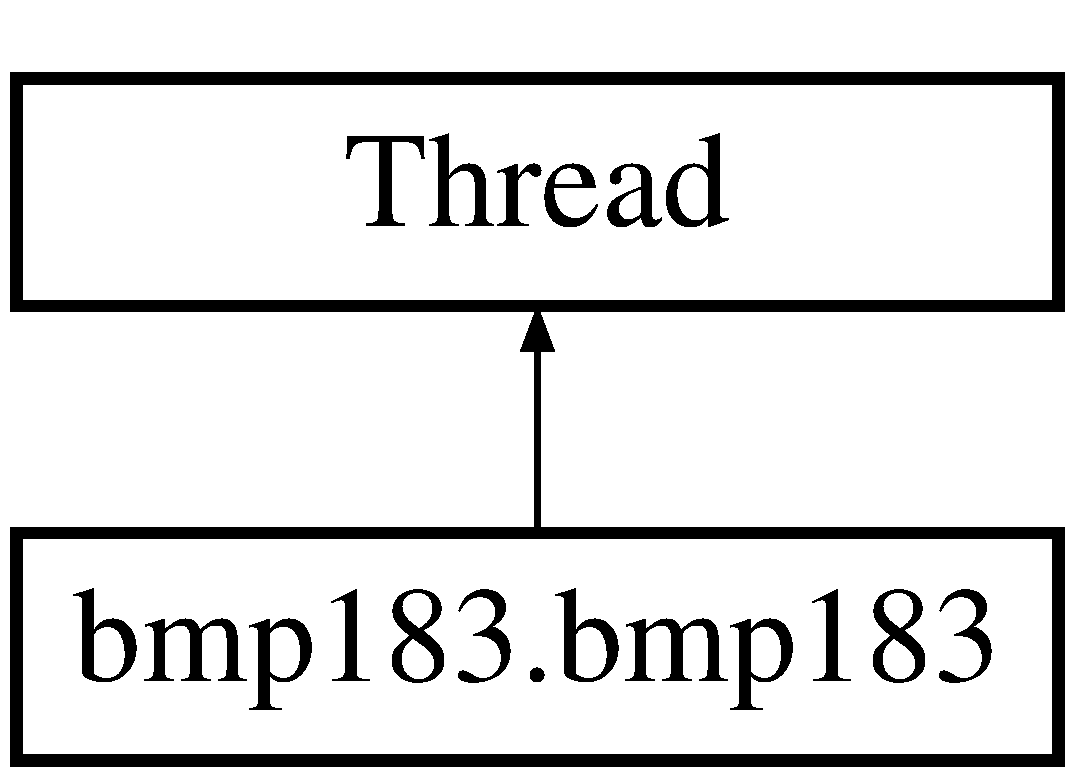
\includegraphics[height=2.000000cm]{classbmp183_1_1bmp183}
\end{center}
\end{figure}
\subsection*{Public Member Functions}
\begin{DoxyCompactItemize}
\item 
def \hyperlink{classbmp183_1_1bmp183_abff9456bd2e262738b3d2bc8d75fb931}{\+\_\+\+\_\+init\+\_\+\+\_\+} (self, \hyperlink{classbmp183_1_1bmp183_af2e228fbb767e51461bc3b906c95e08a}{simulate}=False)
\item 
def \hyperlink{classbmp183_1_1bmp183_a5e6acda0bca8df5d68f673959a75023a}{get\+\_\+data} (self)
\item 
def \hyperlink{classbmp183_1_1bmp183_aa95ba9d2ee3ea621fa744e0084929065}{stop} (self)
\item 
def \hyperlink{classbmp183_1_1bmp183_a07d23f8009ce9777dfe09ae86520d090}{\+\_\+\+\_\+del\+\_\+\+\_\+} (self)
\item 
def \hyperlink{classbmp183_1_1bmp183_ac97968b3dac366872efb1c35a0075894}{set\+\_\+up\+\_\+gpio} (self)
\item 
def \hyperlink{classbmp183_1_1bmp183_a7c318f9ad88f503eef530c5eb0bec53f}{cleanup\+\_\+gpio} (self)
\item 
def \hyperlink{classbmp183_1_1bmp183_aebeb011deb88334ca6117f9c2c1e6a25}{read\+\_\+byte} (self, addr)
\item 
def \hyperlink{classbmp183_1_1bmp183_acb489a2b4069a82181778661ab03a253}{read\+\_\+word} (self, addr, extra\+\_\+bits=0)
\item 
def \hyperlink{classbmp183_1_1bmp183_a3a1505772511584be7c7c520d6401510}{write\+\_\+byte} (self, addr, value)
\item 
def \hyperlink{classbmp183_1_1bmp183_aa9f341ec4f04763a41fa286a5e63ca25}{spi\+\_\+transfer} (self, addr, value, rw, length)
\item 
def \hyperlink{classbmp183_1_1bmp183_a62162d8715be0b61e81e36ebcefb2a6c}{read\+\_\+calibration\+\_\+data} (self)
\item 
def \hyperlink{classbmp183_1_1bmp183_aa22da0e9cc7ec3fad2a4df816dc29f27}{measure\+\_\+temperature} (self)
\item 
def \hyperlink{classbmp183_1_1bmp183_ae2cd9be902c9da687f3cb80b6d041a21}{measure\+\_\+pressure} (self)
\item 
def \hyperlink{classbmp183_1_1bmp183_ad3925b2b055181dde2f192861dc1214f}{calculate\+\_\+pressure} (self)
\item 
def \hyperlink{classbmp183_1_1bmp183_ae9ff54fa23b6657aaf46acb662a8a1fc}{calculate\+\_\+temperature} (self)
\item 
def \hyperlink{classbmp183_1_1bmp183_aabd7c1509c165bdb1433b3dcb4540da0}{stop\+\_\+measurement} (self)
\item 
def \hyperlink{classbmp183_1_1bmp183_a1cd6a20d6910bd850cd98df4c0ddb7d7}{run} (self)
\item 
def \hyperlink{classbmp183_1_1bmp183_a5eecb87615765a4614e670fbd8b3d015}{kalman\+\_\+setup} (self)
\item 
def \hyperlink{classbmp183_1_1bmp183_a97339b46ef50f4f8d870bdb84dcdea2e}{kalman\+\_\+update} (self)
\end{DoxyCompactItemize}
\subsection*{Public Attributes}
\begin{DoxyCompactItemize}
\item 
\hyperlink{classbmp183_1_1bmp183_ac87bb026ca991eff94a53cf63aa86e88}{l}
\item 
\hyperlink{classbmp183_1_1bmp183_af2e228fbb767e51461bc3b906c95e08a}{simulate}
\item 
\hyperlink{classbmp183_1_1bmp183_a1d2933cf8ce9bbd7abf24bb1f28ab4ee}{sensor\+\_\+ready}
\item 
\hyperlink{classbmp183_1_1bmp183_a4838c002f7a24208181603b7a7971153}{running}
\item 
\hyperlink{classbmp183_1_1bmp183_a5f1d5197f3919e316f43334abbf79445}{first\+\_\+run}
\item 
\hyperlink{classbmp183_1_1bmp183_aaca2ad4c3eba2c305cbd3f971d85dcc2}{measurement\+\_\+delay}
\item 
\hyperlink{classbmp183_1_1bmp183_a272d8d0103d7e896ec2e5ab9b5d9bf68}{temperature}
\item 
\hyperlink{classbmp183_1_1bmp183_ab5582d76691ab9fd6a6ae580be6db9a9}{temperature\+\_\+max\+\_\+delta}
\item 
\hyperlink{classbmp183_1_1bmp183_aa47a54b94ef26b77e7d0e139f9417871}{pressure}
\item 
\hyperlink{classbmp183_1_1bmp183_a1b8e100aed6d3a6f3cfeb92b66a60af1}{pressure\+\_\+unfiltered}
\item 
\hyperlink{classbmp183_1_1bmp183_a0d61f8d98e702bd5a9dd1f5f5a09727c}{S\+CK}
\item 
\hyperlink{classbmp183_1_1bmp183_a6c1a17425e5f0a326f71017871ae3414}{S\+DO}
\item 
\hyperlink{classbmp183_1_1bmp183_aa659c8f1c1a30c0c165fe3f76b2ad5f2}{S\+DI}
\item 
\hyperlink{classbmp183_1_1bmp183_a359725ee2f7c74747e696f9798edb73a}{CS}
\item 
\hyperlink{classbmp183_1_1bmp183_a35cbcb30fbc22936680ab2f007f08c89}{delay}
\item 
\hyperlink{classbmp183_1_1bmp183_a82d67582b79b80d138db18a07fb5d351}{A\+C1}
\item 
\hyperlink{classbmp183_1_1bmp183_a85de00ba5a69ec2aef7d3b425d690671}{A\+C2}
\item 
\hyperlink{classbmp183_1_1bmp183_a9975c3c482a0e3b428f7f425f3e5c461}{A\+C3}
\item 
\hyperlink{classbmp183_1_1bmp183_ab4d3b53ffef90a7d3cfc7f60d2704265}{A\+C4}
\item 
\hyperlink{classbmp183_1_1bmp183_ad88e001d0701dc7cf3a48729eb8150e5}{A\+C5}
\item 
\hyperlink{classbmp183_1_1bmp183_a701bb46a4a32843305e0fd27aabaf43a}{A\+C6}
\item 
\hyperlink{classbmp183_1_1bmp183_a2a42039ccc9ae970620b57b740003753}{B1}
\item 
\hyperlink{classbmp183_1_1bmp183_a888b45737b8318b9d7a15e7a0cef4ce8}{B2}
\item 
\hyperlink{classbmp183_1_1bmp183_afb8d2d137be4de89c83dec10b2c40e80}{MB}
\item 
\hyperlink{classbmp183_1_1bmp183_a8dfa9c55987e86febf9c0b470527c5ae}{MC}
\item 
\hyperlink{classbmp183_1_1bmp183_a02b235142116033fcc0e854d2a2ebed8}{MD}
\item 
\hyperlink{classbmp183_1_1bmp183_a4ad4aeaa8cd60eebc072b8c6e42454b9}{UT}
\item 
\hyperlink{classbmp183_1_1bmp183_a5e0825f49b6206d3c4e201ad08e14ce1}{UP}
\item 
\hyperlink{classbmp183_1_1bmp183_a9c2123df95d8752304b44fade6db4cbe}{B6}
\item 
\hyperlink{classbmp183_1_1bmp183_af82d03ff5a63a36141365fb1d9691e11}{B3}
\item 
\hyperlink{classbmp183_1_1bmp183_aec9db96888f829bf866e9f474d7cd6c3}{B4}
\item 
\hyperlink{classbmp183_1_1bmp183_ae3a6e214efff1d4bfe89bbcbf77d1624}{B7}
\item 
\hyperlink{classbmp183_1_1bmp183_aa058849b3003d9b05e7b74843ce79099}{B5}
\item 
\hyperlink{classbmp183_1_1bmp183_aab882410fdb59bd2da0b167da450dcd0}{T}
\item 
\hyperlink{classbmp183_1_1bmp183_a207931f830d20f4da639ad0c6506ed3a}{Q}
\item 
\hyperlink{classbmp183_1_1bmp183_af45af8b2e2c5a21a54c0f257ec26b05e}{pressure\+\_\+estimate}
\item 
\hyperlink{classbmp183_1_1bmp183_a3ae9e6b9a95f8ec27b99a0f4e67de35b}{P}
\item 
\hyperlink{classbmp183_1_1bmp183_a287856d34cd623db00c2796699eae1cc}{pressure\+\_\+estimate\+\_\+previous}
\item 
\hyperlink{classbmp183_1_1bmp183_acff61d68ac312ea2bef1300aa3fbe0d3}{P\+\_\+previous}
\item 
\hyperlink{classbmp183_1_1bmp183_a50f080ed87360a55dc316b4006576a8b}{K}
\item 
\hyperlink{classbmp183_1_1bmp183_a5d9d15ca620299f6046bce90b78b28ee}{R}
\end{DoxyCompactItemize}
\subsection*{Static Public Attributes}
\begin{DoxyCompactItemize}
\item 
dictionary \hyperlink{classbmp183_1_1bmp183_ab907f6f3c1aef0a95df7f653c613f79f}{B\+M\+P183\+\_\+\+R\+EG}
\item 
dictionary \hyperlink{classbmp183_1_1bmp183_adfc4b0a2ebdb9b408e1fe027c94aae30}{B\+M\+P183\+\_\+\+C\+MD}
\end{DoxyCompactItemize}


\subsection{Constructor \& Destructor Documentation}
\mbox{\Hypertarget{classbmp183_1_1bmp183_abff9456bd2e262738b3d2bc8d75fb931}\label{classbmp183_1_1bmp183_abff9456bd2e262738b3d2bc8d75fb931}} 
\index{bmp183\+::bmp183@{bmp183\+::bmp183}!\+\_\+\+\_\+init\+\_\+\+\_\+@{\+\_\+\+\_\+init\+\_\+\+\_\+}}
\index{\+\_\+\+\_\+init\+\_\+\+\_\+@{\+\_\+\+\_\+init\+\_\+\+\_\+}!bmp183\+::bmp183@{bmp183\+::bmp183}}
\subsubsection{\texorpdfstring{\+\_\+\+\_\+init\+\_\+\+\_\+()}{\_\_init\_\_()}}
{\footnotesize\ttfamily def bmp183.\+bmp183.\+\_\+\+\_\+init\+\_\+\+\_\+ (\begin{DoxyParamCaption}\item[{}]{self,  }\item[{}]{simulate = {\ttfamily False} }\end{DoxyParamCaption})}

\mbox{\Hypertarget{classbmp183_1_1bmp183_a07d23f8009ce9777dfe09ae86520d090}\label{classbmp183_1_1bmp183_a07d23f8009ce9777dfe09ae86520d090}} 
\index{bmp183\+::bmp183@{bmp183\+::bmp183}!\+\_\+\+\_\+del\+\_\+\+\_\+@{\+\_\+\+\_\+del\+\_\+\+\_\+}}
\index{\+\_\+\+\_\+del\+\_\+\+\_\+@{\+\_\+\+\_\+del\+\_\+\+\_\+}!bmp183\+::bmp183@{bmp183\+::bmp183}}
\subsubsection{\texorpdfstring{\+\_\+\+\_\+del\+\_\+\+\_\+()}{\_\_del\_\_()}}
{\footnotesize\ttfamily def bmp183.\+bmp183.\+\_\+\+\_\+del\+\_\+\+\_\+ (\begin{DoxyParamCaption}\item[{}]{self }\end{DoxyParamCaption})}



\subsection{Member Function Documentation}
\mbox{\Hypertarget{classbmp183_1_1bmp183_ad3925b2b055181dde2f192861dc1214f}\label{classbmp183_1_1bmp183_ad3925b2b055181dde2f192861dc1214f}} 
\index{bmp183\+::bmp183@{bmp183\+::bmp183}!calculate\+\_\+pressure@{calculate\+\_\+pressure}}
\index{calculate\+\_\+pressure@{calculate\+\_\+pressure}!bmp183\+::bmp183@{bmp183\+::bmp183}}
\subsubsection{\texorpdfstring{calculate\+\_\+pressure()}{calculate\_pressure()}}
{\footnotesize\ttfamily def bmp183.\+bmp183.\+calculate\+\_\+pressure (\begin{DoxyParamCaption}\item[{}]{self }\end{DoxyParamCaption})}

\mbox{\Hypertarget{classbmp183_1_1bmp183_ae9ff54fa23b6657aaf46acb662a8a1fc}\label{classbmp183_1_1bmp183_ae9ff54fa23b6657aaf46acb662a8a1fc}} 
\index{bmp183\+::bmp183@{bmp183\+::bmp183}!calculate\+\_\+temperature@{calculate\+\_\+temperature}}
\index{calculate\+\_\+temperature@{calculate\+\_\+temperature}!bmp183\+::bmp183@{bmp183\+::bmp183}}
\subsubsection{\texorpdfstring{calculate\+\_\+temperature()}{calculate\_temperature()}}
{\footnotesize\ttfamily def bmp183.\+bmp183.\+calculate\+\_\+temperature (\begin{DoxyParamCaption}\item[{}]{self }\end{DoxyParamCaption})}

\mbox{\Hypertarget{classbmp183_1_1bmp183_a7c318f9ad88f503eef530c5eb0bec53f}\label{classbmp183_1_1bmp183_a7c318f9ad88f503eef530c5eb0bec53f}} 
\index{bmp183\+::bmp183@{bmp183\+::bmp183}!cleanup\+\_\+gpio@{cleanup\+\_\+gpio}}
\index{cleanup\+\_\+gpio@{cleanup\+\_\+gpio}!bmp183\+::bmp183@{bmp183\+::bmp183}}
\subsubsection{\texorpdfstring{cleanup\+\_\+gpio()}{cleanup\_gpio()}}
{\footnotesize\ttfamily def bmp183.\+bmp183.\+cleanup\+\_\+gpio (\begin{DoxyParamCaption}\item[{}]{self }\end{DoxyParamCaption})}

\mbox{\Hypertarget{classbmp183_1_1bmp183_a5e6acda0bca8df5d68f673959a75023a}\label{classbmp183_1_1bmp183_a5e6acda0bca8df5d68f673959a75023a}} 
\index{bmp183\+::bmp183@{bmp183\+::bmp183}!get\+\_\+data@{get\+\_\+data}}
\index{get\+\_\+data@{get\+\_\+data}!bmp183\+::bmp183@{bmp183\+::bmp183}}
\subsubsection{\texorpdfstring{get\+\_\+data()}{get\_data()}}
{\footnotesize\ttfamily def bmp183.\+bmp183.\+get\+\_\+data (\begin{DoxyParamCaption}\item[{}]{self }\end{DoxyParamCaption})}

\mbox{\Hypertarget{classbmp183_1_1bmp183_a5eecb87615765a4614e670fbd8b3d015}\label{classbmp183_1_1bmp183_a5eecb87615765a4614e670fbd8b3d015}} 
\index{bmp183\+::bmp183@{bmp183\+::bmp183}!kalman\+\_\+setup@{kalman\+\_\+setup}}
\index{kalman\+\_\+setup@{kalman\+\_\+setup}!bmp183\+::bmp183@{bmp183\+::bmp183}}
\subsubsection{\texorpdfstring{kalman\+\_\+setup()}{kalman\_setup()}}
{\footnotesize\ttfamily def bmp183.\+bmp183.\+kalman\+\_\+setup (\begin{DoxyParamCaption}\item[{}]{self }\end{DoxyParamCaption})}

\mbox{\Hypertarget{classbmp183_1_1bmp183_a97339b46ef50f4f8d870bdb84dcdea2e}\label{classbmp183_1_1bmp183_a97339b46ef50f4f8d870bdb84dcdea2e}} 
\index{bmp183\+::bmp183@{bmp183\+::bmp183}!kalman\+\_\+update@{kalman\+\_\+update}}
\index{kalman\+\_\+update@{kalman\+\_\+update}!bmp183\+::bmp183@{bmp183\+::bmp183}}
\subsubsection{\texorpdfstring{kalman\+\_\+update()}{kalman\_update()}}
{\footnotesize\ttfamily def bmp183.\+bmp183.\+kalman\+\_\+update (\begin{DoxyParamCaption}\item[{}]{self }\end{DoxyParamCaption})}

\mbox{\Hypertarget{classbmp183_1_1bmp183_ae2cd9be902c9da687f3cb80b6d041a21}\label{classbmp183_1_1bmp183_ae2cd9be902c9da687f3cb80b6d041a21}} 
\index{bmp183\+::bmp183@{bmp183\+::bmp183}!measure\+\_\+pressure@{measure\+\_\+pressure}}
\index{measure\+\_\+pressure@{measure\+\_\+pressure}!bmp183\+::bmp183@{bmp183\+::bmp183}}
\subsubsection{\texorpdfstring{measure\+\_\+pressure()}{measure\_pressure()}}
{\footnotesize\ttfamily def bmp183.\+bmp183.\+measure\+\_\+pressure (\begin{DoxyParamCaption}\item[{}]{self }\end{DoxyParamCaption})}

\mbox{\Hypertarget{classbmp183_1_1bmp183_aa22da0e9cc7ec3fad2a4df816dc29f27}\label{classbmp183_1_1bmp183_aa22da0e9cc7ec3fad2a4df816dc29f27}} 
\index{bmp183\+::bmp183@{bmp183\+::bmp183}!measure\+\_\+temperature@{measure\+\_\+temperature}}
\index{measure\+\_\+temperature@{measure\+\_\+temperature}!bmp183\+::bmp183@{bmp183\+::bmp183}}
\subsubsection{\texorpdfstring{measure\+\_\+temperature()}{measure\_temperature()}}
{\footnotesize\ttfamily def bmp183.\+bmp183.\+measure\+\_\+temperature (\begin{DoxyParamCaption}\item[{}]{self }\end{DoxyParamCaption})}

\mbox{\Hypertarget{classbmp183_1_1bmp183_aebeb011deb88334ca6117f9c2c1e6a25}\label{classbmp183_1_1bmp183_aebeb011deb88334ca6117f9c2c1e6a25}} 
\index{bmp183\+::bmp183@{bmp183\+::bmp183}!read\+\_\+byte@{read\+\_\+byte}}
\index{read\+\_\+byte@{read\+\_\+byte}!bmp183\+::bmp183@{bmp183\+::bmp183}}
\subsubsection{\texorpdfstring{read\+\_\+byte()}{read\_byte()}}
{\footnotesize\ttfamily def bmp183.\+bmp183.\+read\+\_\+byte (\begin{DoxyParamCaption}\item[{}]{self,  }\item[{}]{addr }\end{DoxyParamCaption})}

\mbox{\Hypertarget{classbmp183_1_1bmp183_a62162d8715be0b61e81e36ebcefb2a6c}\label{classbmp183_1_1bmp183_a62162d8715be0b61e81e36ebcefb2a6c}} 
\index{bmp183\+::bmp183@{bmp183\+::bmp183}!read\+\_\+calibration\+\_\+data@{read\+\_\+calibration\+\_\+data}}
\index{read\+\_\+calibration\+\_\+data@{read\+\_\+calibration\+\_\+data}!bmp183\+::bmp183@{bmp183\+::bmp183}}
\subsubsection{\texorpdfstring{read\+\_\+calibration\+\_\+data()}{read\_calibration\_data()}}
{\footnotesize\ttfamily def bmp183.\+bmp183.\+read\+\_\+calibration\+\_\+data (\begin{DoxyParamCaption}\item[{}]{self }\end{DoxyParamCaption})}

\mbox{\Hypertarget{classbmp183_1_1bmp183_acb489a2b4069a82181778661ab03a253}\label{classbmp183_1_1bmp183_acb489a2b4069a82181778661ab03a253}} 
\index{bmp183\+::bmp183@{bmp183\+::bmp183}!read\+\_\+word@{read\+\_\+word}}
\index{read\+\_\+word@{read\+\_\+word}!bmp183\+::bmp183@{bmp183\+::bmp183}}
\subsubsection{\texorpdfstring{read\+\_\+word()}{read\_word()}}
{\footnotesize\ttfamily def bmp183.\+bmp183.\+read\+\_\+word (\begin{DoxyParamCaption}\item[{}]{self,  }\item[{}]{addr,  }\item[{}]{extra\+\_\+bits = {\ttfamily 0} }\end{DoxyParamCaption})}

\mbox{\Hypertarget{classbmp183_1_1bmp183_a1cd6a20d6910bd850cd98df4c0ddb7d7}\label{classbmp183_1_1bmp183_a1cd6a20d6910bd850cd98df4c0ddb7d7}} 
\index{bmp183\+::bmp183@{bmp183\+::bmp183}!run@{run}}
\index{run@{run}!bmp183\+::bmp183@{bmp183\+::bmp183}}
\subsubsection{\texorpdfstring{run()}{run()}}
{\footnotesize\ttfamily def bmp183.\+bmp183.\+run (\begin{DoxyParamCaption}\item[{}]{self }\end{DoxyParamCaption})}

\mbox{\Hypertarget{classbmp183_1_1bmp183_ac97968b3dac366872efb1c35a0075894}\label{classbmp183_1_1bmp183_ac97968b3dac366872efb1c35a0075894}} 
\index{bmp183\+::bmp183@{bmp183\+::bmp183}!set\+\_\+up\+\_\+gpio@{set\+\_\+up\+\_\+gpio}}
\index{set\+\_\+up\+\_\+gpio@{set\+\_\+up\+\_\+gpio}!bmp183\+::bmp183@{bmp183\+::bmp183}}
\subsubsection{\texorpdfstring{set\+\_\+up\+\_\+gpio()}{set\_up\_gpio()}}
{\footnotesize\ttfamily def bmp183.\+bmp183.\+set\+\_\+up\+\_\+gpio (\begin{DoxyParamCaption}\item[{}]{self }\end{DoxyParamCaption})}

\mbox{\Hypertarget{classbmp183_1_1bmp183_aa9f341ec4f04763a41fa286a5e63ca25}\label{classbmp183_1_1bmp183_aa9f341ec4f04763a41fa286a5e63ca25}} 
\index{bmp183\+::bmp183@{bmp183\+::bmp183}!spi\+\_\+transfer@{spi\+\_\+transfer}}
\index{spi\+\_\+transfer@{spi\+\_\+transfer}!bmp183\+::bmp183@{bmp183\+::bmp183}}
\subsubsection{\texorpdfstring{spi\+\_\+transfer()}{spi\_transfer()}}
{\footnotesize\ttfamily def bmp183.\+bmp183.\+spi\+\_\+transfer (\begin{DoxyParamCaption}\item[{}]{self,  }\item[{}]{addr,  }\item[{}]{value,  }\item[{}]{rw,  }\item[{}]{length }\end{DoxyParamCaption})}

\mbox{\Hypertarget{classbmp183_1_1bmp183_aa95ba9d2ee3ea621fa744e0084929065}\label{classbmp183_1_1bmp183_aa95ba9d2ee3ea621fa744e0084929065}} 
\index{bmp183\+::bmp183@{bmp183\+::bmp183}!stop@{stop}}
\index{stop@{stop}!bmp183\+::bmp183@{bmp183\+::bmp183}}
\subsubsection{\texorpdfstring{stop()}{stop()}}
{\footnotesize\ttfamily def bmp183.\+bmp183.\+stop (\begin{DoxyParamCaption}\item[{}]{self }\end{DoxyParamCaption})}

\mbox{\Hypertarget{classbmp183_1_1bmp183_aabd7c1509c165bdb1433b3dcb4540da0}\label{classbmp183_1_1bmp183_aabd7c1509c165bdb1433b3dcb4540da0}} 
\index{bmp183\+::bmp183@{bmp183\+::bmp183}!stop\+\_\+measurement@{stop\+\_\+measurement}}
\index{stop\+\_\+measurement@{stop\+\_\+measurement}!bmp183\+::bmp183@{bmp183\+::bmp183}}
\subsubsection{\texorpdfstring{stop\+\_\+measurement()}{stop\_measurement()}}
{\footnotesize\ttfamily def bmp183.\+bmp183.\+stop\+\_\+measurement (\begin{DoxyParamCaption}\item[{}]{self }\end{DoxyParamCaption})}

\mbox{\Hypertarget{classbmp183_1_1bmp183_a3a1505772511584be7c7c520d6401510}\label{classbmp183_1_1bmp183_a3a1505772511584be7c7c520d6401510}} 
\index{bmp183\+::bmp183@{bmp183\+::bmp183}!write\+\_\+byte@{write\+\_\+byte}}
\index{write\+\_\+byte@{write\+\_\+byte}!bmp183\+::bmp183@{bmp183\+::bmp183}}
\subsubsection{\texorpdfstring{write\+\_\+byte()}{write\_byte()}}
{\footnotesize\ttfamily def bmp183.\+bmp183.\+write\+\_\+byte (\begin{DoxyParamCaption}\item[{}]{self,  }\item[{}]{addr,  }\item[{}]{value }\end{DoxyParamCaption})}



\subsection{Member Data Documentation}
\mbox{\Hypertarget{classbmp183_1_1bmp183_a82d67582b79b80d138db18a07fb5d351}\label{classbmp183_1_1bmp183_a82d67582b79b80d138db18a07fb5d351}} 
\index{bmp183\+::bmp183@{bmp183\+::bmp183}!A\+C1@{A\+C1}}
\index{A\+C1@{A\+C1}!bmp183\+::bmp183@{bmp183\+::bmp183}}
\subsubsection{\texorpdfstring{A\+C1}{AC1}}
{\footnotesize\ttfamily bmp183.\+bmp183.\+A\+C1}

\mbox{\Hypertarget{classbmp183_1_1bmp183_a85de00ba5a69ec2aef7d3b425d690671}\label{classbmp183_1_1bmp183_a85de00ba5a69ec2aef7d3b425d690671}} 
\index{bmp183\+::bmp183@{bmp183\+::bmp183}!A\+C2@{A\+C2}}
\index{A\+C2@{A\+C2}!bmp183\+::bmp183@{bmp183\+::bmp183}}
\subsubsection{\texorpdfstring{A\+C2}{AC2}}
{\footnotesize\ttfamily bmp183.\+bmp183.\+A\+C2}

\mbox{\Hypertarget{classbmp183_1_1bmp183_a9975c3c482a0e3b428f7f425f3e5c461}\label{classbmp183_1_1bmp183_a9975c3c482a0e3b428f7f425f3e5c461}} 
\index{bmp183\+::bmp183@{bmp183\+::bmp183}!A\+C3@{A\+C3}}
\index{A\+C3@{A\+C3}!bmp183\+::bmp183@{bmp183\+::bmp183}}
\subsubsection{\texorpdfstring{A\+C3}{AC3}}
{\footnotesize\ttfamily bmp183.\+bmp183.\+A\+C3}

\mbox{\Hypertarget{classbmp183_1_1bmp183_ab4d3b53ffef90a7d3cfc7f60d2704265}\label{classbmp183_1_1bmp183_ab4d3b53ffef90a7d3cfc7f60d2704265}} 
\index{bmp183\+::bmp183@{bmp183\+::bmp183}!A\+C4@{A\+C4}}
\index{A\+C4@{A\+C4}!bmp183\+::bmp183@{bmp183\+::bmp183}}
\subsubsection{\texorpdfstring{A\+C4}{AC4}}
{\footnotesize\ttfamily bmp183.\+bmp183.\+A\+C4}

\mbox{\Hypertarget{classbmp183_1_1bmp183_ad88e001d0701dc7cf3a48729eb8150e5}\label{classbmp183_1_1bmp183_ad88e001d0701dc7cf3a48729eb8150e5}} 
\index{bmp183\+::bmp183@{bmp183\+::bmp183}!A\+C5@{A\+C5}}
\index{A\+C5@{A\+C5}!bmp183\+::bmp183@{bmp183\+::bmp183}}
\subsubsection{\texorpdfstring{A\+C5}{AC5}}
{\footnotesize\ttfamily bmp183.\+bmp183.\+A\+C5}

\mbox{\Hypertarget{classbmp183_1_1bmp183_a701bb46a4a32843305e0fd27aabaf43a}\label{classbmp183_1_1bmp183_a701bb46a4a32843305e0fd27aabaf43a}} 
\index{bmp183\+::bmp183@{bmp183\+::bmp183}!A\+C6@{A\+C6}}
\index{A\+C6@{A\+C6}!bmp183\+::bmp183@{bmp183\+::bmp183}}
\subsubsection{\texorpdfstring{A\+C6}{AC6}}
{\footnotesize\ttfamily bmp183.\+bmp183.\+A\+C6}

\mbox{\Hypertarget{classbmp183_1_1bmp183_a2a42039ccc9ae970620b57b740003753}\label{classbmp183_1_1bmp183_a2a42039ccc9ae970620b57b740003753}} 
\index{bmp183\+::bmp183@{bmp183\+::bmp183}!B1@{B1}}
\index{B1@{B1}!bmp183\+::bmp183@{bmp183\+::bmp183}}
\subsubsection{\texorpdfstring{B1}{B1}}
{\footnotesize\ttfamily bmp183.\+bmp183.\+B1}

\mbox{\Hypertarget{classbmp183_1_1bmp183_a888b45737b8318b9d7a15e7a0cef4ce8}\label{classbmp183_1_1bmp183_a888b45737b8318b9d7a15e7a0cef4ce8}} 
\index{bmp183\+::bmp183@{bmp183\+::bmp183}!B2@{B2}}
\index{B2@{B2}!bmp183\+::bmp183@{bmp183\+::bmp183}}
\subsubsection{\texorpdfstring{B2}{B2}}
{\footnotesize\ttfamily bmp183.\+bmp183.\+B2}

\mbox{\Hypertarget{classbmp183_1_1bmp183_af82d03ff5a63a36141365fb1d9691e11}\label{classbmp183_1_1bmp183_af82d03ff5a63a36141365fb1d9691e11}} 
\index{bmp183\+::bmp183@{bmp183\+::bmp183}!B3@{B3}}
\index{B3@{B3}!bmp183\+::bmp183@{bmp183\+::bmp183}}
\subsubsection{\texorpdfstring{B3}{B3}}
{\footnotesize\ttfamily bmp183.\+bmp183.\+B3}

\mbox{\Hypertarget{classbmp183_1_1bmp183_aec9db96888f829bf866e9f474d7cd6c3}\label{classbmp183_1_1bmp183_aec9db96888f829bf866e9f474d7cd6c3}} 
\index{bmp183\+::bmp183@{bmp183\+::bmp183}!B4@{B4}}
\index{B4@{B4}!bmp183\+::bmp183@{bmp183\+::bmp183}}
\subsubsection{\texorpdfstring{B4}{B4}}
{\footnotesize\ttfamily bmp183.\+bmp183.\+B4}

\mbox{\Hypertarget{classbmp183_1_1bmp183_aa058849b3003d9b05e7b74843ce79099}\label{classbmp183_1_1bmp183_aa058849b3003d9b05e7b74843ce79099}} 
\index{bmp183\+::bmp183@{bmp183\+::bmp183}!B5@{B5}}
\index{B5@{B5}!bmp183\+::bmp183@{bmp183\+::bmp183}}
\subsubsection{\texorpdfstring{B5}{B5}}
{\footnotesize\ttfamily bmp183.\+bmp183.\+B5}

\mbox{\Hypertarget{classbmp183_1_1bmp183_a9c2123df95d8752304b44fade6db4cbe}\label{classbmp183_1_1bmp183_a9c2123df95d8752304b44fade6db4cbe}} 
\index{bmp183\+::bmp183@{bmp183\+::bmp183}!B6@{B6}}
\index{B6@{B6}!bmp183\+::bmp183@{bmp183\+::bmp183}}
\subsubsection{\texorpdfstring{B6}{B6}}
{\footnotesize\ttfamily bmp183.\+bmp183.\+B6}

\mbox{\Hypertarget{classbmp183_1_1bmp183_ae3a6e214efff1d4bfe89bbcbf77d1624}\label{classbmp183_1_1bmp183_ae3a6e214efff1d4bfe89bbcbf77d1624}} 
\index{bmp183\+::bmp183@{bmp183\+::bmp183}!B7@{B7}}
\index{B7@{B7}!bmp183\+::bmp183@{bmp183\+::bmp183}}
\subsubsection{\texorpdfstring{B7}{B7}}
{\footnotesize\ttfamily bmp183.\+bmp183.\+B7}

\mbox{\Hypertarget{classbmp183_1_1bmp183_adfc4b0a2ebdb9b408e1fe027c94aae30}\label{classbmp183_1_1bmp183_adfc4b0a2ebdb9b408e1fe027c94aae30}} 
\index{bmp183\+::bmp183@{bmp183\+::bmp183}!B\+M\+P183\+\_\+\+C\+MD@{B\+M\+P183\+\_\+\+C\+MD}}
\index{B\+M\+P183\+\_\+\+C\+MD@{B\+M\+P183\+\_\+\+C\+MD}!bmp183\+::bmp183@{bmp183\+::bmp183}}
\subsubsection{\texorpdfstring{B\+M\+P183\+\_\+\+C\+MD}{BMP183\_CMD}}
{\footnotesize\ttfamily dictionary bmp183.\+bmp183.\+B\+M\+P183\+\_\+\+C\+MD\hspace{0.3cm}{\ttfamily [static]}}

{\bfseries Initial value\+:}
\begin{DoxyCode}
=  \{
        \textcolor{comment}{#@ Chip ID Value fixed to 0x55. Useful to check if communication works}
        \textcolor{stringliteral}{'ID\_VALUE'}: 0x55,

        \textcolor{comment}{# SPI bit to indicate READ or WRITE operation}
        \textcolor{stringliteral}{'READWRITE'}: 0x80,

        \textcolor{comment}{# Read TEMPERATURE, Wait time 4.5 ms}
        \textcolor{stringliteral}{'TEMP'}: 0x2E,
        \textcolor{stringliteral}{'TEMP\_WAIT'}: 0.0045,

        \textcolor{comment}{# Read PRESSURE}
        \textcolor{stringliteral}{'PRESS'}: 0x34,  \textcolor{comment}{# 001}

        \textcolor{comment}{# PRESSURE reading modes}
        \textcolor{comment}{# Example usage: (PRESS || (OVERSAMPLE\_2 << 4)}
        \textcolor{stringliteral}{'OVERSAMPLE\_0'}: 0x0,  \textcolor{comment}{# ultra low power, no oversampling, wait time 4.5 ms}
        \textcolor{stringliteral}{'OVERSAMPLE\_0\_WAIT'}: 0.0045,
        \textcolor{stringliteral}{'OVERSAMPLE\_1'}: 0x1,  \textcolor{comment}{# standard, 2 internal samples, wait time 7.5 ms}
        \textcolor{stringliteral}{'OVERSAMPLE\_1\_WAIT'}: 0.0075,
        \textcolor{stringliteral}{'OVERSAMPLE\_2'}: 0x2,  \textcolor{comment}{# high resolution, 4 internal samples, wait time 13.5 ms}
        \textcolor{stringliteral}{'OVERSAMPLE\_2\_WAIT'}: 0.0135,
        \textcolor{stringliteral}{'OVERSAMPLE\_3'}: 0x3,  \textcolor{comment}{# ultra high resolution, 8 internal samples, Wait time 25.5 ms}
        \textcolor{stringliteral}{'OVERSAMPLE\_3\_WAIT'}: 0.0255,
    \}
\end{DoxyCode}
\mbox{\Hypertarget{classbmp183_1_1bmp183_ab907f6f3c1aef0a95df7f653c613f79f}\label{classbmp183_1_1bmp183_ab907f6f3c1aef0a95df7f653c613f79f}} 
\index{bmp183\+::bmp183@{bmp183\+::bmp183}!B\+M\+P183\+\_\+\+R\+EG@{B\+M\+P183\+\_\+\+R\+EG}}
\index{B\+M\+P183\+\_\+\+R\+EG@{B\+M\+P183\+\_\+\+R\+EG}!bmp183\+::bmp183@{bmp183\+::bmp183}}
\subsubsection{\texorpdfstring{B\+M\+P183\+\_\+\+R\+EG}{BMP183\_REG}}
{\footnotesize\ttfamily dictionary bmp183.\+bmp183.\+B\+M\+P183\+\_\+\+R\+EG\hspace{0.3cm}{\ttfamily [static]}}

{\bfseries Initial value\+:}
\begin{DoxyCode}
=  \{
        \textcolor{comment}{#@ Calibration data}
        \textcolor{stringliteral}{'CAL\_AC1'}: 0xAA,
        \textcolor{stringliteral}{'CAL\_AC2'}: 0xAC,
        \textcolor{stringliteral}{'CAL\_AC3'}: 0xAE,
        \textcolor{stringliteral}{'CAL\_AC4'}: 0xB0,
        \textcolor{stringliteral}{'CAL\_AC5'}: 0xB2,
        \textcolor{stringliteral}{'CAL\_AC6'}: 0xB4,
        \textcolor{stringliteral}{'CAL\_B1'}: 0xB6,
        \textcolor{stringliteral}{'CAL\_B2'}: 0xB8,
        \textcolor{stringliteral}{'CAL\_MB'}: 0xBA,
        \textcolor{stringliteral}{'CAL\_MC'}: 0xBC,
        \textcolor{stringliteral}{'CAL\_MD'}: 0xBE,

        \textcolor{comment}{#@ Chip ID. Value fixed to 0x55. Useful to check if communication works}
        \textcolor{stringliteral}{'ID'}: 0xD0,
        \textcolor{stringliteral}{'ID\_VALUE'}: 0x55,

        \textcolor{comment}{#@ VER Undocumented}
        \textcolor{stringliteral}{'VER'}: 0xD1,

        \textcolor{comment}{#@ SOFT\_RESET Write only. If set to 0xB6, will perform the same sequence as power on reset.}
        \textcolor{stringliteral}{'SOFT\_RESET'}: 0xE0,

        \textcolor{comment}{#@ CTRL\_MEAS Controls measurements}
        \textcolor{stringliteral}{'CTRL\_MEAS'}: 0xF4,

        \textcolor{comment}{#@ DATA}
        \textcolor{stringliteral}{'DATA'}: 0xF6,
    \}
\end{DoxyCode}
\mbox{\Hypertarget{classbmp183_1_1bmp183_a359725ee2f7c74747e696f9798edb73a}\label{classbmp183_1_1bmp183_a359725ee2f7c74747e696f9798edb73a}} 
\index{bmp183\+::bmp183@{bmp183\+::bmp183}!CS@{CS}}
\index{CS@{CS}!bmp183\+::bmp183@{bmp183\+::bmp183}}
\subsubsection{\texorpdfstring{CS}{CS}}
{\footnotesize\ttfamily bmp183.\+bmp183.\+CS}

\mbox{\Hypertarget{classbmp183_1_1bmp183_a35cbcb30fbc22936680ab2f007f08c89}\label{classbmp183_1_1bmp183_a35cbcb30fbc22936680ab2f007f08c89}} 
\index{bmp183\+::bmp183@{bmp183\+::bmp183}!delay@{delay}}
\index{delay@{delay}!bmp183\+::bmp183@{bmp183\+::bmp183}}
\subsubsection{\texorpdfstring{delay}{delay}}
{\footnotesize\ttfamily bmp183.\+bmp183.\+delay}

\mbox{\Hypertarget{classbmp183_1_1bmp183_a5f1d5197f3919e316f43334abbf79445}\label{classbmp183_1_1bmp183_a5f1d5197f3919e316f43334abbf79445}} 
\index{bmp183\+::bmp183@{bmp183\+::bmp183}!first\+\_\+run@{first\+\_\+run}}
\index{first\+\_\+run@{first\+\_\+run}!bmp183\+::bmp183@{bmp183\+::bmp183}}
\subsubsection{\texorpdfstring{first\+\_\+run}{first\_run}}
{\footnotesize\ttfamily bmp183.\+bmp183.\+first\+\_\+run}

\mbox{\Hypertarget{classbmp183_1_1bmp183_a50f080ed87360a55dc316b4006576a8b}\label{classbmp183_1_1bmp183_a50f080ed87360a55dc316b4006576a8b}} 
\index{bmp183\+::bmp183@{bmp183\+::bmp183}!K@{K}}
\index{K@{K}!bmp183\+::bmp183@{bmp183\+::bmp183}}
\subsubsection{\texorpdfstring{K}{K}}
{\footnotesize\ttfamily bmp183.\+bmp183.\+K}

\mbox{\Hypertarget{classbmp183_1_1bmp183_ac87bb026ca991eff94a53cf63aa86e88}\label{classbmp183_1_1bmp183_ac87bb026ca991eff94a53cf63aa86e88}} 
\index{bmp183\+::bmp183@{bmp183\+::bmp183}!l@{l}}
\index{l@{l}!bmp183\+::bmp183@{bmp183\+::bmp183}}
\subsubsection{\texorpdfstring{l}{l}}
{\footnotesize\ttfamily bmp183.\+bmp183.\+l}

\mbox{\Hypertarget{classbmp183_1_1bmp183_afb8d2d137be4de89c83dec10b2c40e80}\label{classbmp183_1_1bmp183_afb8d2d137be4de89c83dec10b2c40e80}} 
\index{bmp183\+::bmp183@{bmp183\+::bmp183}!MB@{MB}}
\index{MB@{MB}!bmp183\+::bmp183@{bmp183\+::bmp183}}
\subsubsection{\texorpdfstring{MB}{MB}}
{\footnotesize\ttfamily bmp183.\+bmp183.\+MB}

\mbox{\Hypertarget{classbmp183_1_1bmp183_a8dfa9c55987e86febf9c0b470527c5ae}\label{classbmp183_1_1bmp183_a8dfa9c55987e86febf9c0b470527c5ae}} 
\index{bmp183\+::bmp183@{bmp183\+::bmp183}!MC@{MC}}
\index{MC@{MC}!bmp183\+::bmp183@{bmp183\+::bmp183}}
\subsubsection{\texorpdfstring{MC}{MC}}
{\footnotesize\ttfamily bmp183.\+bmp183.\+MC}

\mbox{\Hypertarget{classbmp183_1_1bmp183_a02b235142116033fcc0e854d2a2ebed8}\label{classbmp183_1_1bmp183_a02b235142116033fcc0e854d2a2ebed8}} 
\index{bmp183\+::bmp183@{bmp183\+::bmp183}!MD@{MD}}
\index{MD@{MD}!bmp183\+::bmp183@{bmp183\+::bmp183}}
\subsubsection{\texorpdfstring{MD}{MD}}
{\footnotesize\ttfamily bmp183.\+bmp183.\+MD}

\mbox{\Hypertarget{classbmp183_1_1bmp183_aaca2ad4c3eba2c305cbd3f971d85dcc2}\label{classbmp183_1_1bmp183_aaca2ad4c3eba2c305cbd3f971d85dcc2}} 
\index{bmp183\+::bmp183@{bmp183\+::bmp183}!measurement\+\_\+delay@{measurement\+\_\+delay}}
\index{measurement\+\_\+delay@{measurement\+\_\+delay}!bmp183\+::bmp183@{bmp183\+::bmp183}}
\subsubsection{\texorpdfstring{measurement\+\_\+delay}{measurement\_delay}}
{\footnotesize\ttfamily bmp183.\+bmp183.\+measurement\+\_\+delay}

\mbox{\Hypertarget{classbmp183_1_1bmp183_a3ae9e6b9a95f8ec27b99a0f4e67de35b}\label{classbmp183_1_1bmp183_a3ae9e6b9a95f8ec27b99a0f4e67de35b}} 
\index{bmp183\+::bmp183@{bmp183\+::bmp183}!P@{P}}
\index{P@{P}!bmp183\+::bmp183@{bmp183\+::bmp183}}
\subsubsection{\texorpdfstring{P}{P}}
{\footnotesize\ttfamily bmp183.\+bmp183.\+P}

\mbox{\Hypertarget{classbmp183_1_1bmp183_acff61d68ac312ea2bef1300aa3fbe0d3}\label{classbmp183_1_1bmp183_acff61d68ac312ea2bef1300aa3fbe0d3}} 
\index{bmp183\+::bmp183@{bmp183\+::bmp183}!P\+\_\+previous@{P\+\_\+previous}}
\index{P\+\_\+previous@{P\+\_\+previous}!bmp183\+::bmp183@{bmp183\+::bmp183}}
\subsubsection{\texorpdfstring{P\+\_\+previous}{P\_previous}}
{\footnotesize\ttfamily bmp183.\+bmp183.\+P\+\_\+previous}

\mbox{\Hypertarget{classbmp183_1_1bmp183_aa47a54b94ef26b77e7d0e139f9417871}\label{classbmp183_1_1bmp183_aa47a54b94ef26b77e7d0e139f9417871}} 
\index{bmp183\+::bmp183@{bmp183\+::bmp183}!pressure@{pressure}}
\index{pressure@{pressure}!bmp183\+::bmp183@{bmp183\+::bmp183}}
\subsubsection{\texorpdfstring{pressure}{pressure}}
{\footnotesize\ttfamily bmp183.\+bmp183.\+pressure}

\mbox{\Hypertarget{classbmp183_1_1bmp183_af45af8b2e2c5a21a54c0f257ec26b05e}\label{classbmp183_1_1bmp183_af45af8b2e2c5a21a54c0f257ec26b05e}} 
\index{bmp183\+::bmp183@{bmp183\+::bmp183}!pressure\+\_\+estimate@{pressure\+\_\+estimate}}
\index{pressure\+\_\+estimate@{pressure\+\_\+estimate}!bmp183\+::bmp183@{bmp183\+::bmp183}}
\subsubsection{\texorpdfstring{pressure\+\_\+estimate}{pressure\_estimate}}
{\footnotesize\ttfamily bmp183.\+bmp183.\+pressure\+\_\+estimate}

\mbox{\Hypertarget{classbmp183_1_1bmp183_a287856d34cd623db00c2796699eae1cc}\label{classbmp183_1_1bmp183_a287856d34cd623db00c2796699eae1cc}} 
\index{bmp183\+::bmp183@{bmp183\+::bmp183}!pressure\+\_\+estimate\+\_\+previous@{pressure\+\_\+estimate\+\_\+previous}}
\index{pressure\+\_\+estimate\+\_\+previous@{pressure\+\_\+estimate\+\_\+previous}!bmp183\+::bmp183@{bmp183\+::bmp183}}
\subsubsection{\texorpdfstring{pressure\+\_\+estimate\+\_\+previous}{pressure\_estimate\_previous}}
{\footnotesize\ttfamily bmp183.\+bmp183.\+pressure\+\_\+estimate\+\_\+previous}

\mbox{\Hypertarget{classbmp183_1_1bmp183_a1b8e100aed6d3a6f3cfeb92b66a60af1}\label{classbmp183_1_1bmp183_a1b8e100aed6d3a6f3cfeb92b66a60af1}} 
\index{bmp183\+::bmp183@{bmp183\+::bmp183}!pressure\+\_\+unfiltered@{pressure\+\_\+unfiltered}}
\index{pressure\+\_\+unfiltered@{pressure\+\_\+unfiltered}!bmp183\+::bmp183@{bmp183\+::bmp183}}
\subsubsection{\texorpdfstring{pressure\+\_\+unfiltered}{pressure\_unfiltered}}
{\footnotesize\ttfamily bmp183.\+bmp183.\+pressure\+\_\+unfiltered}

\mbox{\Hypertarget{classbmp183_1_1bmp183_a207931f830d20f4da639ad0c6506ed3a}\label{classbmp183_1_1bmp183_a207931f830d20f4da639ad0c6506ed3a}} 
\index{bmp183\+::bmp183@{bmp183\+::bmp183}!Q@{Q}}
\index{Q@{Q}!bmp183\+::bmp183@{bmp183\+::bmp183}}
\subsubsection{\texorpdfstring{Q}{Q}}
{\footnotesize\ttfamily bmp183.\+bmp183.\+Q}

\mbox{\Hypertarget{classbmp183_1_1bmp183_a5d9d15ca620299f6046bce90b78b28ee}\label{classbmp183_1_1bmp183_a5d9d15ca620299f6046bce90b78b28ee}} 
\index{bmp183\+::bmp183@{bmp183\+::bmp183}!R@{R}}
\index{R@{R}!bmp183\+::bmp183@{bmp183\+::bmp183}}
\subsubsection{\texorpdfstring{R}{R}}
{\footnotesize\ttfamily bmp183.\+bmp183.\+R}

\mbox{\Hypertarget{classbmp183_1_1bmp183_a4838c002f7a24208181603b7a7971153}\label{classbmp183_1_1bmp183_a4838c002f7a24208181603b7a7971153}} 
\index{bmp183\+::bmp183@{bmp183\+::bmp183}!running@{running}}
\index{running@{running}!bmp183\+::bmp183@{bmp183\+::bmp183}}
\subsubsection{\texorpdfstring{running}{running}}
{\footnotesize\ttfamily bmp183.\+bmp183.\+running}

\mbox{\Hypertarget{classbmp183_1_1bmp183_a0d61f8d98e702bd5a9dd1f5f5a09727c}\label{classbmp183_1_1bmp183_a0d61f8d98e702bd5a9dd1f5f5a09727c}} 
\index{bmp183\+::bmp183@{bmp183\+::bmp183}!S\+CK@{S\+CK}}
\index{S\+CK@{S\+CK}!bmp183\+::bmp183@{bmp183\+::bmp183}}
\subsubsection{\texorpdfstring{S\+CK}{SCK}}
{\footnotesize\ttfamily bmp183.\+bmp183.\+S\+CK}

\mbox{\Hypertarget{classbmp183_1_1bmp183_aa659c8f1c1a30c0c165fe3f76b2ad5f2}\label{classbmp183_1_1bmp183_aa659c8f1c1a30c0c165fe3f76b2ad5f2}} 
\index{bmp183\+::bmp183@{bmp183\+::bmp183}!S\+DI@{S\+DI}}
\index{S\+DI@{S\+DI}!bmp183\+::bmp183@{bmp183\+::bmp183}}
\subsubsection{\texorpdfstring{S\+DI}{SDI}}
{\footnotesize\ttfamily bmp183.\+bmp183.\+S\+DI}

\mbox{\Hypertarget{classbmp183_1_1bmp183_a6c1a17425e5f0a326f71017871ae3414}\label{classbmp183_1_1bmp183_a6c1a17425e5f0a326f71017871ae3414}} 
\index{bmp183\+::bmp183@{bmp183\+::bmp183}!S\+DO@{S\+DO}}
\index{S\+DO@{S\+DO}!bmp183\+::bmp183@{bmp183\+::bmp183}}
\subsubsection{\texorpdfstring{S\+DO}{SDO}}
{\footnotesize\ttfamily bmp183.\+bmp183.\+S\+DO}

\mbox{\Hypertarget{classbmp183_1_1bmp183_a1d2933cf8ce9bbd7abf24bb1f28ab4ee}\label{classbmp183_1_1bmp183_a1d2933cf8ce9bbd7abf24bb1f28ab4ee}} 
\index{bmp183\+::bmp183@{bmp183\+::bmp183}!sensor\+\_\+ready@{sensor\+\_\+ready}}
\index{sensor\+\_\+ready@{sensor\+\_\+ready}!bmp183\+::bmp183@{bmp183\+::bmp183}}
\subsubsection{\texorpdfstring{sensor\+\_\+ready}{sensor\_ready}}
{\footnotesize\ttfamily bmp183.\+bmp183.\+sensor\+\_\+ready}

\mbox{\Hypertarget{classbmp183_1_1bmp183_af2e228fbb767e51461bc3b906c95e08a}\label{classbmp183_1_1bmp183_af2e228fbb767e51461bc3b906c95e08a}} 
\index{bmp183\+::bmp183@{bmp183\+::bmp183}!simulate@{simulate}}
\index{simulate@{simulate}!bmp183\+::bmp183@{bmp183\+::bmp183}}
\subsubsection{\texorpdfstring{simulate}{simulate}}
{\footnotesize\ttfamily bmp183.\+bmp183.\+simulate}

\mbox{\Hypertarget{classbmp183_1_1bmp183_aab882410fdb59bd2da0b167da450dcd0}\label{classbmp183_1_1bmp183_aab882410fdb59bd2da0b167da450dcd0}} 
\index{bmp183\+::bmp183@{bmp183\+::bmp183}!T@{T}}
\index{T@{T}!bmp183\+::bmp183@{bmp183\+::bmp183}}
\subsubsection{\texorpdfstring{T}{T}}
{\footnotesize\ttfamily bmp183.\+bmp183.\+T}

\mbox{\Hypertarget{classbmp183_1_1bmp183_a272d8d0103d7e896ec2e5ab9b5d9bf68}\label{classbmp183_1_1bmp183_a272d8d0103d7e896ec2e5ab9b5d9bf68}} 
\index{bmp183\+::bmp183@{bmp183\+::bmp183}!temperature@{temperature}}
\index{temperature@{temperature}!bmp183\+::bmp183@{bmp183\+::bmp183}}
\subsubsection{\texorpdfstring{temperature}{temperature}}
{\footnotesize\ttfamily bmp183.\+bmp183.\+temperature}

\mbox{\Hypertarget{classbmp183_1_1bmp183_ab5582d76691ab9fd6a6ae580be6db9a9}\label{classbmp183_1_1bmp183_ab5582d76691ab9fd6a6ae580be6db9a9}} 
\index{bmp183\+::bmp183@{bmp183\+::bmp183}!temperature\+\_\+max\+\_\+delta@{temperature\+\_\+max\+\_\+delta}}
\index{temperature\+\_\+max\+\_\+delta@{temperature\+\_\+max\+\_\+delta}!bmp183\+::bmp183@{bmp183\+::bmp183}}
\subsubsection{\texorpdfstring{temperature\+\_\+max\+\_\+delta}{temperature\_max\_delta}}
{\footnotesize\ttfamily bmp183.\+bmp183.\+temperature\+\_\+max\+\_\+delta}

\mbox{\Hypertarget{classbmp183_1_1bmp183_a5e0825f49b6206d3c4e201ad08e14ce1}\label{classbmp183_1_1bmp183_a5e0825f49b6206d3c4e201ad08e14ce1}} 
\index{bmp183\+::bmp183@{bmp183\+::bmp183}!UP@{UP}}
\index{UP@{UP}!bmp183\+::bmp183@{bmp183\+::bmp183}}
\subsubsection{\texorpdfstring{UP}{UP}}
{\footnotesize\ttfamily bmp183.\+bmp183.\+UP}

\mbox{\Hypertarget{classbmp183_1_1bmp183_a4ad4aeaa8cd60eebc072b8c6e42454b9}\label{classbmp183_1_1bmp183_a4ad4aeaa8cd60eebc072b8c6e42454b9}} 
\index{bmp183\+::bmp183@{bmp183\+::bmp183}!UT@{UT}}
\index{UT@{UT}!bmp183\+::bmp183@{bmp183\+::bmp183}}
\subsubsection{\texorpdfstring{UT}{UT}}
{\footnotesize\ttfamily bmp183.\+bmp183.\+UT}



The documentation for this class was generated from the following file\+:\begin{DoxyCompactItemize}
\item 
src/\hyperlink{bmp183_8py}{bmp183.\+py}\end{DoxyCompactItemize}

\hypertarget{classconfig_1_1config}{}\section{config.\+config Class Reference}
\label{classconfig_1_1config}\index{config.\+config@{config.\+config}}
Inheritance diagram for config.\+config\+:\begin{figure}[H]
\begin{center}
\leavevmode
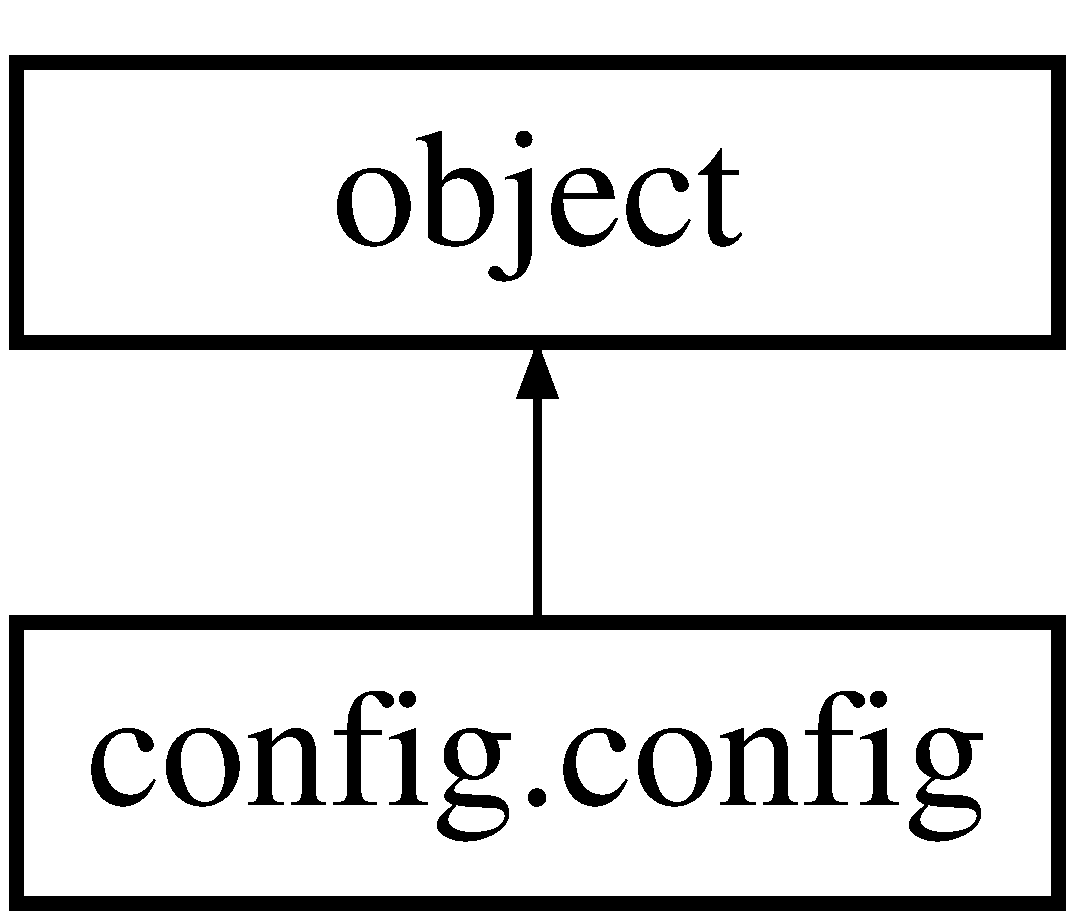
\includegraphics[height=2.000000cm]{classconfig_1_1config}
\end{center}
\end{figure}
\subsection*{Public Member Functions}
\begin{DoxyCompactItemize}
\item 
def \hyperlink{classconfig_1_1config_a2f19893c6121bbacf28e3f4fafe93f08}{\+\_\+\+\_\+init\+\_\+\+\_\+} (self, \hyperlink{classconfig_1_1config_ac3bf336655093c3b3dcf8d24027e9b6e}{occ}, \hyperlink{classconfig_1_1config_ae2a8159c1071eb51bd9200540126ebc4}{config\+\_\+file\+\_\+path}, \hyperlink{classconfig_1_1config_a553062767fb374889c2f51f31be593d1}{base\+\_\+config\+\_\+file\+\_\+path})
\item 
def \hyperlink{classconfig_1_1config_a7dc5250998fe2899548ae676fbf6af51}{read\+\_\+config} (self)
\item 
def \hyperlink{classconfig_1_1config_a595ae0b2abc4883e8d703eb63570d0be}{write\+\_\+config} (self)
\end{DoxyCompactItemize}
\subsection*{Public Attributes}
\begin{DoxyCompactItemize}
\item 
\hyperlink{classconfig_1_1config_a98de02645a6c4a2cbcfce4cf22d548b8}{l}
\item 
\hyperlink{classconfig_1_1config_ac3bf336655093c3b3dcf8d24027e9b6e}{occ}
\item 
\hyperlink{classconfig_1_1config_aa4d251490aa3957ddf73d409800a89f9}{rp}
\item 
\hyperlink{classconfig_1_1config_ae2a8159c1071eb51bd9200540126ebc4}{config\+\_\+file\+\_\+path}
\item 
\hyperlink{classconfig_1_1config_a553062767fb374889c2f51f31be593d1}{base\+\_\+config\+\_\+file\+\_\+path}
\item 
\hyperlink{classconfig_1_1config_a5908fb27351049f2fb2bf3b12935b55b}{config}
\end{DoxyCompactItemize}


\subsection{Constructor \& Destructor Documentation}
\mbox{\Hypertarget{classconfig_1_1config_a2f19893c6121bbacf28e3f4fafe93f08}\label{classconfig_1_1config_a2f19893c6121bbacf28e3f4fafe93f08}} 
\index{config\+::config@{config\+::config}!\+\_\+\+\_\+init\+\_\+\+\_\+@{\+\_\+\+\_\+init\+\_\+\+\_\+}}
\index{\+\_\+\+\_\+init\+\_\+\+\_\+@{\+\_\+\+\_\+init\+\_\+\+\_\+}!config\+::config@{config\+::config}}
\subsubsection{\texorpdfstring{\+\_\+\+\_\+init\+\_\+\+\_\+()}{\_\_init\_\_()}}
{\footnotesize\ttfamily def config.\+config.\+\_\+\+\_\+init\+\_\+\+\_\+ (\begin{DoxyParamCaption}\item[{}]{self,  }\item[{}]{occ,  }\item[{}]{config\+\_\+file\+\_\+path,  }\item[{}]{base\+\_\+config\+\_\+file\+\_\+path }\end{DoxyParamCaption})}



\subsection{Member Function Documentation}
\mbox{\Hypertarget{classconfig_1_1config_a7dc5250998fe2899548ae676fbf6af51}\label{classconfig_1_1config_a7dc5250998fe2899548ae676fbf6af51}} 
\index{config\+::config@{config\+::config}!read\+\_\+config@{read\+\_\+config}}
\index{read\+\_\+config@{read\+\_\+config}!config\+::config@{config\+::config}}
\subsubsection{\texorpdfstring{read\+\_\+config()}{read\_config()}}
{\footnotesize\ttfamily def config.\+config.\+read\+\_\+config (\begin{DoxyParamCaption}\item[{}]{self }\end{DoxyParamCaption})}

\mbox{\Hypertarget{classconfig_1_1config_a595ae0b2abc4883e8d703eb63570d0be}\label{classconfig_1_1config_a595ae0b2abc4883e8d703eb63570d0be}} 
\index{config\+::config@{config\+::config}!write\+\_\+config@{write\+\_\+config}}
\index{write\+\_\+config@{write\+\_\+config}!config\+::config@{config\+::config}}
\subsubsection{\texorpdfstring{write\+\_\+config()}{write\_config()}}
{\footnotesize\ttfamily def config.\+config.\+write\+\_\+config (\begin{DoxyParamCaption}\item[{}]{self }\end{DoxyParamCaption})}



\subsection{Member Data Documentation}
\mbox{\Hypertarget{classconfig_1_1config_a553062767fb374889c2f51f31be593d1}\label{classconfig_1_1config_a553062767fb374889c2f51f31be593d1}} 
\index{config\+::config@{config\+::config}!base\+\_\+config\+\_\+file\+\_\+path@{base\+\_\+config\+\_\+file\+\_\+path}}
\index{base\+\_\+config\+\_\+file\+\_\+path@{base\+\_\+config\+\_\+file\+\_\+path}!config\+::config@{config\+::config}}
\subsubsection{\texorpdfstring{base\+\_\+config\+\_\+file\+\_\+path}{base\_config\_file\_path}}
{\footnotesize\ttfamily config.\+config.\+base\+\_\+config\+\_\+file\+\_\+path}

\mbox{\Hypertarget{classconfig_1_1config_a5908fb27351049f2fb2bf3b12935b55b}\label{classconfig_1_1config_a5908fb27351049f2fb2bf3b12935b55b}} 
\index{config\+::config@{config\+::config}!config@{config}}
\index{config@{config}!config\+::config@{config\+::config}}
\subsubsection{\texorpdfstring{config}{config}}
{\footnotesize\ttfamily config.\+config.\+config}

\mbox{\Hypertarget{classconfig_1_1config_ae2a8159c1071eb51bd9200540126ebc4}\label{classconfig_1_1config_ae2a8159c1071eb51bd9200540126ebc4}} 
\index{config\+::config@{config\+::config}!config\+\_\+file\+\_\+path@{config\+\_\+file\+\_\+path}}
\index{config\+\_\+file\+\_\+path@{config\+\_\+file\+\_\+path}!config\+::config@{config\+::config}}
\subsubsection{\texorpdfstring{config\+\_\+file\+\_\+path}{config\_file\_path}}
{\footnotesize\ttfamily config.\+config.\+config\+\_\+file\+\_\+path}

\mbox{\Hypertarget{classconfig_1_1config_a98de02645a6c4a2cbcfce4cf22d548b8}\label{classconfig_1_1config_a98de02645a6c4a2cbcfce4cf22d548b8}} 
\index{config\+::config@{config\+::config}!l@{l}}
\index{l@{l}!config\+::config@{config\+::config}}
\subsubsection{\texorpdfstring{l}{l}}
{\footnotesize\ttfamily config.\+config.\+l}

\mbox{\Hypertarget{classconfig_1_1config_ac3bf336655093c3b3dcf8d24027e9b6e}\label{classconfig_1_1config_ac3bf336655093c3b3dcf8d24027e9b6e}} 
\index{config\+::config@{config\+::config}!occ@{occ}}
\index{occ@{occ}!config\+::config@{config\+::config}}
\subsubsection{\texorpdfstring{occ}{occ}}
{\footnotesize\ttfamily config.\+config.\+occ}

\mbox{\Hypertarget{classconfig_1_1config_aa4d251490aa3957ddf73d409800a89f9}\label{classconfig_1_1config_aa4d251490aa3957ddf73d409800a89f9}} 
\index{config\+::config@{config\+::config}!rp@{rp}}
\index{rp@{rp}!config\+::config@{config\+::config}}
\subsubsection{\texorpdfstring{rp}{rp}}
{\footnotesize\ttfamily config.\+config.\+rp}



The documentation for this class was generated from the following file\+:\begin{DoxyCompactItemize}
\item 
src/\hyperlink{config_8py}{config.\+py}\end{DoxyCompactItemize}

\hypertarget{classble__sc_1_1CSC__Delegate}{}\section{ble\+\_\+sc.\+C\+S\+C\+\_\+\+Delegate Class Reference}
\label{classble__sc_1_1CSC__Delegate}\index{ble\+\_\+sc.\+C\+S\+C\+\_\+\+Delegate@{ble\+\_\+sc.\+C\+S\+C\+\_\+\+Delegate}}
Inheritance diagram for ble\+\_\+sc.\+C\+S\+C\+\_\+\+Delegate\+:\begin{figure}[H]
\begin{center}
\leavevmode
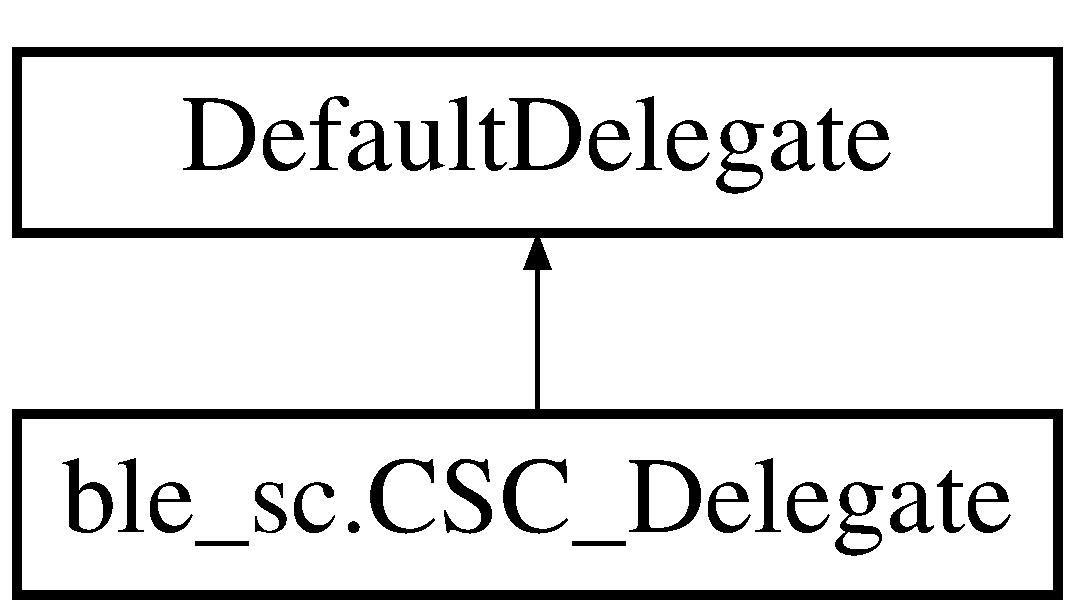
\includegraphics[height=2.000000cm]{classble__sc_1_1CSC__Delegate}
\end{center}
\end{figure}
\subsection*{Public Member Functions}
\begin{DoxyCompactItemize}
\item 
def \hyperlink{classble__sc_1_1CSC__Delegate_a343f74589886a83496cca797a4d9d2ab}{\+\_\+\+\_\+init\+\_\+\+\_\+} (self)
\item 
def \hyperlink{classble__sc_1_1CSC__Delegate_a8f8eb71e6870e9bb5f3fbd36d0ccfda9}{handle\+Notification} (self, c\+Handle, data)
\end{DoxyCompactItemize}
\subsection*{Public Attributes}
\begin{DoxyCompactItemize}
\item 
\hyperlink{classble__sc_1_1CSC__Delegate_af237ae7177e1dba023617ab7c68f103a}{l}
\item 
\hyperlink{classble__sc_1_1CSC__Delegate_a4bd2c809d7123ec3b4d24510a7c29995}{wheel\+\_\+time\+\_\+stamp}
\item 
\hyperlink{classble__sc_1_1CSC__Delegate_a6cf7441d1a9f64d4589f264969dbba31}{wheel\+\_\+cumul}
\item 
\hyperlink{classble__sc_1_1CSC__Delegate_ab3d37c1828f03c4deb67a42294576718}{wheel\+\_\+last\+\_\+time\+\_\+event}
\item 
\hyperlink{classble__sc_1_1CSC__Delegate_ab0615eadb968070c25825660225c8230}{wheel\+\_\+last\+\_\+time\+\_\+delta}
\item 
\hyperlink{classble__sc_1_1CSC__Delegate_a9dbf98de41a570429328322ba71c351c}{wheel\+\_\+rev\+\_\+time}
\item 
\hyperlink{classble__sc_1_1CSC__Delegate_a1a9a94381e98c2b570ef10ba08088310}{cadence\+\_\+time\+\_\+stamp}
\item 
\hyperlink{classble__sc_1_1CSC__Delegate_a848195bccd1c79f19252061c5bf78864}{crank\+\_\+cumul}
\item 
\hyperlink{classble__sc_1_1CSC__Delegate_ad0e8adcc1155c16cb1be6c06484ed81b}{crank\+\_\+last\+\_\+time\+\_\+event}
\item 
\hyperlink{classble__sc_1_1CSC__Delegate_a12c08f59680dafbf3bb4f195e869230a}{crank\+\_\+last\+\_\+time\+\_\+delta}
\item 
\hyperlink{classble__sc_1_1CSC__Delegate_afff8a85491dfa34563af524d349c6828}{crank\+\_\+rev\+\_\+time}
\item 
\hyperlink{classble__sc_1_1CSC__Delegate_aa1160185d046f02b63558e5ffe4b8bad}{cadence}
\end{DoxyCompactItemize}
\subsection*{Static Public Attributes}
\begin{DoxyCompactItemize}
\item 
int \hyperlink{classble__sc_1_1CSC__Delegate_ac635e545ea7af14713237553b0096211}{W\+H\+E\+E\+L\+\_\+\+R\+E\+V\+\_\+\+D\+A\+T\+A\+\_\+\+P\+R\+E\+S\+E\+NT} = 0x01
\item 
int \hyperlink{classble__sc_1_1CSC__Delegate_abdfb5d122283851cd8efd460209dacde}{C\+R\+A\+N\+K\+\_\+\+R\+E\+V\+\_\+\+D\+A\+T\+A\+\_\+\+P\+R\+E\+S\+E\+NT} = 0x02
\end{DoxyCompactItemize}


\subsection{Constructor \& Destructor Documentation}
\mbox{\Hypertarget{classble__sc_1_1CSC__Delegate_a343f74589886a83496cca797a4d9d2ab}\label{classble__sc_1_1CSC__Delegate_a343f74589886a83496cca797a4d9d2ab}} 
\index{ble\+\_\+sc\+::\+C\+S\+C\+\_\+\+Delegate@{ble\+\_\+sc\+::\+C\+S\+C\+\_\+\+Delegate}!\+\_\+\+\_\+init\+\_\+\+\_\+@{\+\_\+\+\_\+init\+\_\+\+\_\+}}
\index{\+\_\+\+\_\+init\+\_\+\+\_\+@{\+\_\+\+\_\+init\+\_\+\+\_\+}!ble\+\_\+sc\+::\+C\+S\+C\+\_\+\+Delegate@{ble\+\_\+sc\+::\+C\+S\+C\+\_\+\+Delegate}}
\subsubsection{\texorpdfstring{\+\_\+\+\_\+init\+\_\+\+\_\+()}{\_\_init\_\_()}}
{\footnotesize\ttfamily def ble\+\_\+sc.\+C\+S\+C\+\_\+\+Delegate.\+\_\+\+\_\+init\+\_\+\+\_\+ (\begin{DoxyParamCaption}\item[{}]{self }\end{DoxyParamCaption})}



\subsection{Member Function Documentation}
\mbox{\Hypertarget{classble__sc_1_1CSC__Delegate_a8f8eb71e6870e9bb5f3fbd36d0ccfda9}\label{classble__sc_1_1CSC__Delegate_a8f8eb71e6870e9bb5f3fbd36d0ccfda9}} 
\index{ble\+\_\+sc\+::\+C\+S\+C\+\_\+\+Delegate@{ble\+\_\+sc\+::\+C\+S\+C\+\_\+\+Delegate}!handle\+Notification@{handle\+Notification}}
\index{handle\+Notification@{handle\+Notification}!ble\+\_\+sc\+::\+C\+S\+C\+\_\+\+Delegate@{ble\+\_\+sc\+::\+C\+S\+C\+\_\+\+Delegate}}
\subsubsection{\texorpdfstring{handle\+Notification()}{handleNotification()}}
{\footnotesize\ttfamily def ble\+\_\+sc.\+C\+S\+C\+\_\+\+Delegate.\+handle\+Notification (\begin{DoxyParamCaption}\item[{}]{self,  }\item[{}]{c\+Handle,  }\item[{}]{data }\end{DoxyParamCaption})}



\subsection{Member Data Documentation}
\mbox{\Hypertarget{classble__sc_1_1CSC__Delegate_aa1160185d046f02b63558e5ffe4b8bad}\label{classble__sc_1_1CSC__Delegate_aa1160185d046f02b63558e5ffe4b8bad}} 
\index{ble\+\_\+sc\+::\+C\+S\+C\+\_\+\+Delegate@{ble\+\_\+sc\+::\+C\+S\+C\+\_\+\+Delegate}!cadence@{cadence}}
\index{cadence@{cadence}!ble\+\_\+sc\+::\+C\+S\+C\+\_\+\+Delegate@{ble\+\_\+sc\+::\+C\+S\+C\+\_\+\+Delegate}}
\subsubsection{\texorpdfstring{cadence}{cadence}}
{\footnotesize\ttfamily ble\+\_\+sc.\+C\+S\+C\+\_\+\+Delegate.\+cadence}

\mbox{\Hypertarget{classble__sc_1_1CSC__Delegate_a1a9a94381e98c2b570ef10ba08088310}\label{classble__sc_1_1CSC__Delegate_a1a9a94381e98c2b570ef10ba08088310}} 
\index{ble\+\_\+sc\+::\+C\+S\+C\+\_\+\+Delegate@{ble\+\_\+sc\+::\+C\+S\+C\+\_\+\+Delegate}!cadence\+\_\+time\+\_\+stamp@{cadence\+\_\+time\+\_\+stamp}}
\index{cadence\+\_\+time\+\_\+stamp@{cadence\+\_\+time\+\_\+stamp}!ble\+\_\+sc\+::\+C\+S\+C\+\_\+\+Delegate@{ble\+\_\+sc\+::\+C\+S\+C\+\_\+\+Delegate}}
\subsubsection{\texorpdfstring{cadence\+\_\+time\+\_\+stamp}{cadence\_time\_stamp}}
{\footnotesize\ttfamily ble\+\_\+sc.\+C\+S\+C\+\_\+\+Delegate.\+cadence\+\_\+time\+\_\+stamp}

\mbox{\Hypertarget{classble__sc_1_1CSC__Delegate_a848195bccd1c79f19252061c5bf78864}\label{classble__sc_1_1CSC__Delegate_a848195bccd1c79f19252061c5bf78864}} 
\index{ble\+\_\+sc\+::\+C\+S\+C\+\_\+\+Delegate@{ble\+\_\+sc\+::\+C\+S\+C\+\_\+\+Delegate}!crank\+\_\+cumul@{crank\+\_\+cumul}}
\index{crank\+\_\+cumul@{crank\+\_\+cumul}!ble\+\_\+sc\+::\+C\+S\+C\+\_\+\+Delegate@{ble\+\_\+sc\+::\+C\+S\+C\+\_\+\+Delegate}}
\subsubsection{\texorpdfstring{crank\+\_\+cumul}{crank\_cumul}}
{\footnotesize\ttfamily ble\+\_\+sc.\+C\+S\+C\+\_\+\+Delegate.\+crank\+\_\+cumul}

\mbox{\Hypertarget{classble__sc_1_1CSC__Delegate_a12c08f59680dafbf3bb4f195e869230a}\label{classble__sc_1_1CSC__Delegate_a12c08f59680dafbf3bb4f195e869230a}} 
\index{ble\+\_\+sc\+::\+C\+S\+C\+\_\+\+Delegate@{ble\+\_\+sc\+::\+C\+S\+C\+\_\+\+Delegate}!crank\+\_\+last\+\_\+time\+\_\+delta@{crank\+\_\+last\+\_\+time\+\_\+delta}}
\index{crank\+\_\+last\+\_\+time\+\_\+delta@{crank\+\_\+last\+\_\+time\+\_\+delta}!ble\+\_\+sc\+::\+C\+S\+C\+\_\+\+Delegate@{ble\+\_\+sc\+::\+C\+S\+C\+\_\+\+Delegate}}
\subsubsection{\texorpdfstring{crank\+\_\+last\+\_\+time\+\_\+delta}{crank\_last\_time\_delta}}
{\footnotesize\ttfamily ble\+\_\+sc.\+C\+S\+C\+\_\+\+Delegate.\+crank\+\_\+last\+\_\+time\+\_\+delta}

\mbox{\Hypertarget{classble__sc_1_1CSC__Delegate_ad0e8adcc1155c16cb1be6c06484ed81b}\label{classble__sc_1_1CSC__Delegate_ad0e8adcc1155c16cb1be6c06484ed81b}} 
\index{ble\+\_\+sc\+::\+C\+S\+C\+\_\+\+Delegate@{ble\+\_\+sc\+::\+C\+S\+C\+\_\+\+Delegate}!crank\+\_\+last\+\_\+time\+\_\+event@{crank\+\_\+last\+\_\+time\+\_\+event}}
\index{crank\+\_\+last\+\_\+time\+\_\+event@{crank\+\_\+last\+\_\+time\+\_\+event}!ble\+\_\+sc\+::\+C\+S\+C\+\_\+\+Delegate@{ble\+\_\+sc\+::\+C\+S\+C\+\_\+\+Delegate}}
\subsubsection{\texorpdfstring{crank\+\_\+last\+\_\+time\+\_\+event}{crank\_last\_time\_event}}
{\footnotesize\ttfamily ble\+\_\+sc.\+C\+S\+C\+\_\+\+Delegate.\+crank\+\_\+last\+\_\+time\+\_\+event}

\mbox{\Hypertarget{classble__sc_1_1CSC__Delegate_abdfb5d122283851cd8efd460209dacde}\label{classble__sc_1_1CSC__Delegate_abdfb5d122283851cd8efd460209dacde}} 
\index{ble\+\_\+sc\+::\+C\+S\+C\+\_\+\+Delegate@{ble\+\_\+sc\+::\+C\+S\+C\+\_\+\+Delegate}!C\+R\+A\+N\+K\+\_\+\+R\+E\+V\+\_\+\+D\+A\+T\+A\+\_\+\+P\+R\+E\+S\+E\+NT@{C\+R\+A\+N\+K\+\_\+\+R\+E\+V\+\_\+\+D\+A\+T\+A\+\_\+\+P\+R\+E\+S\+E\+NT}}
\index{C\+R\+A\+N\+K\+\_\+\+R\+E\+V\+\_\+\+D\+A\+T\+A\+\_\+\+P\+R\+E\+S\+E\+NT@{C\+R\+A\+N\+K\+\_\+\+R\+E\+V\+\_\+\+D\+A\+T\+A\+\_\+\+P\+R\+E\+S\+E\+NT}!ble\+\_\+sc\+::\+C\+S\+C\+\_\+\+Delegate@{ble\+\_\+sc\+::\+C\+S\+C\+\_\+\+Delegate}}
\subsubsection{\texorpdfstring{C\+R\+A\+N\+K\+\_\+\+R\+E\+V\+\_\+\+D\+A\+T\+A\+\_\+\+P\+R\+E\+S\+E\+NT}{CRANK\_REV\_DATA\_PRESENT}}
{\footnotesize\ttfamily int ble\+\_\+sc.\+C\+S\+C\+\_\+\+Delegate.\+C\+R\+A\+N\+K\+\_\+\+R\+E\+V\+\_\+\+D\+A\+T\+A\+\_\+\+P\+R\+E\+S\+E\+NT = 0x02\hspace{0.3cm}{\ttfamily [static]}}

\mbox{\Hypertarget{classble__sc_1_1CSC__Delegate_afff8a85491dfa34563af524d349c6828}\label{classble__sc_1_1CSC__Delegate_afff8a85491dfa34563af524d349c6828}} 
\index{ble\+\_\+sc\+::\+C\+S\+C\+\_\+\+Delegate@{ble\+\_\+sc\+::\+C\+S\+C\+\_\+\+Delegate}!crank\+\_\+rev\+\_\+time@{crank\+\_\+rev\+\_\+time}}
\index{crank\+\_\+rev\+\_\+time@{crank\+\_\+rev\+\_\+time}!ble\+\_\+sc\+::\+C\+S\+C\+\_\+\+Delegate@{ble\+\_\+sc\+::\+C\+S\+C\+\_\+\+Delegate}}
\subsubsection{\texorpdfstring{crank\+\_\+rev\+\_\+time}{crank\_rev\_time}}
{\footnotesize\ttfamily ble\+\_\+sc.\+C\+S\+C\+\_\+\+Delegate.\+crank\+\_\+rev\+\_\+time}

\mbox{\Hypertarget{classble__sc_1_1CSC__Delegate_af237ae7177e1dba023617ab7c68f103a}\label{classble__sc_1_1CSC__Delegate_af237ae7177e1dba023617ab7c68f103a}} 
\index{ble\+\_\+sc\+::\+C\+S\+C\+\_\+\+Delegate@{ble\+\_\+sc\+::\+C\+S\+C\+\_\+\+Delegate}!l@{l}}
\index{l@{l}!ble\+\_\+sc\+::\+C\+S\+C\+\_\+\+Delegate@{ble\+\_\+sc\+::\+C\+S\+C\+\_\+\+Delegate}}
\subsubsection{\texorpdfstring{l}{l}}
{\footnotesize\ttfamily ble\+\_\+sc.\+C\+S\+C\+\_\+\+Delegate.\+l}

\mbox{\Hypertarget{classble__sc_1_1CSC__Delegate_a6cf7441d1a9f64d4589f264969dbba31}\label{classble__sc_1_1CSC__Delegate_a6cf7441d1a9f64d4589f264969dbba31}} 
\index{ble\+\_\+sc\+::\+C\+S\+C\+\_\+\+Delegate@{ble\+\_\+sc\+::\+C\+S\+C\+\_\+\+Delegate}!wheel\+\_\+cumul@{wheel\+\_\+cumul}}
\index{wheel\+\_\+cumul@{wheel\+\_\+cumul}!ble\+\_\+sc\+::\+C\+S\+C\+\_\+\+Delegate@{ble\+\_\+sc\+::\+C\+S\+C\+\_\+\+Delegate}}
\subsubsection{\texorpdfstring{wheel\+\_\+cumul}{wheel\_cumul}}
{\footnotesize\ttfamily ble\+\_\+sc.\+C\+S\+C\+\_\+\+Delegate.\+wheel\+\_\+cumul}

\mbox{\Hypertarget{classble__sc_1_1CSC__Delegate_ab0615eadb968070c25825660225c8230}\label{classble__sc_1_1CSC__Delegate_ab0615eadb968070c25825660225c8230}} 
\index{ble\+\_\+sc\+::\+C\+S\+C\+\_\+\+Delegate@{ble\+\_\+sc\+::\+C\+S\+C\+\_\+\+Delegate}!wheel\+\_\+last\+\_\+time\+\_\+delta@{wheel\+\_\+last\+\_\+time\+\_\+delta}}
\index{wheel\+\_\+last\+\_\+time\+\_\+delta@{wheel\+\_\+last\+\_\+time\+\_\+delta}!ble\+\_\+sc\+::\+C\+S\+C\+\_\+\+Delegate@{ble\+\_\+sc\+::\+C\+S\+C\+\_\+\+Delegate}}
\subsubsection{\texorpdfstring{wheel\+\_\+last\+\_\+time\+\_\+delta}{wheel\_last\_time\_delta}}
{\footnotesize\ttfamily ble\+\_\+sc.\+C\+S\+C\+\_\+\+Delegate.\+wheel\+\_\+last\+\_\+time\+\_\+delta}

\mbox{\Hypertarget{classble__sc_1_1CSC__Delegate_ab3d37c1828f03c4deb67a42294576718}\label{classble__sc_1_1CSC__Delegate_ab3d37c1828f03c4deb67a42294576718}} 
\index{ble\+\_\+sc\+::\+C\+S\+C\+\_\+\+Delegate@{ble\+\_\+sc\+::\+C\+S\+C\+\_\+\+Delegate}!wheel\+\_\+last\+\_\+time\+\_\+event@{wheel\+\_\+last\+\_\+time\+\_\+event}}
\index{wheel\+\_\+last\+\_\+time\+\_\+event@{wheel\+\_\+last\+\_\+time\+\_\+event}!ble\+\_\+sc\+::\+C\+S\+C\+\_\+\+Delegate@{ble\+\_\+sc\+::\+C\+S\+C\+\_\+\+Delegate}}
\subsubsection{\texorpdfstring{wheel\+\_\+last\+\_\+time\+\_\+event}{wheel\_last\_time\_event}}
{\footnotesize\ttfamily ble\+\_\+sc.\+C\+S\+C\+\_\+\+Delegate.\+wheel\+\_\+last\+\_\+time\+\_\+event}

\mbox{\Hypertarget{classble__sc_1_1CSC__Delegate_ac635e545ea7af14713237553b0096211}\label{classble__sc_1_1CSC__Delegate_ac635e545ea7af14713237553b0096211}} 
\index{ble\+\_\+sc\+::\+C\+S\+C\+\_\+\+Delegate@{ble\+\_\+sc\+::\+C\+S\+C\+\_\+\+Delegate}!W\+H\+E\+E\+L\+\_\+\+R\+E\+V\+\_\+\+D\+A\+T\+A\+\_\+\+P\+R\+E\+S\+E\+NT@{W\+H\+E\+E\+L\+\_\+\+R\+E\+V\+\_\+\+D\+A\+T\+A\+\_\+\+P\+R\+E\+S\+E\+NT}}
\index{W\+H\+E\+E\+L\+\_\+\+R\+E\+V\+\_\+\+D\+A\+T\+A\+\_\+\+P\+R\+E\+S\+E\+NT@{W\+H\+E\+E\+L\+\_\+\+R\+E\+V\+\_\+\+D\+A\+T\+A\+\_\+\+P\+R\+E\+S\+E\+NT}!ble\+\_\+sc\+::\+C\+S\+C\+\_\+\+Delegate@{ble\+\_\+sc\+::\+C\+S\+C\+\_\+\+Delegate}}
\subsubsection{\texorpdfstring{W\+H\+E\+E\+L\+\_\+\+R\+E\+V\+\_\+\+D\+A\+T\+A\+\_\+\+P\+R\+E\+S\+E\+NT}{WHEEL\_REV\_DATA\_PRESENT}}
{\footnotesize\ttfamily int ble\+\_\+sc.\+C\+S\+C\+\_\+\+Delegate.\+W\+H\+E\+E\+L\+\_\+\+R\+E\+V\+\_\+\+D\+A\+T\+A\+\_\+\+P\+R\+E\+S\+E\+NT = 0x01\hspace{0.3cm}{\ttfamily [static]}}

\mbox{\Hypertarget{classble__sc_1_1CSC__Delegate_a9dbf98de41a570429328322ba71c351c}\label{classble__sc_1_1CSC__Delegate_a9dbf98de41a570429328322ba71c351c}} 
\index{ble\+\_\+sc\+::\+C\+S\+C\+\_\+\+Delegate@{ble\+\_\+sc\+::\+C\+S\+C\+\_\+\+Delegate}!wheel\+\_\+rev\+\_\+time@{wheel\+\_\+rev\+\_\+time}}
\index{wheel\+\_\+rev\+\_\+time@{wheel\+\_\+rev\+\_\+time}!ble\+\_\+sc\+::\+C\+S\+C\+\_\+\+Delegate@{ble\+\_\+sc\+::\+C\+S\+C\+\_\+\+Delegate}}
\subsubsection{\texorpdfstring{wheel\+\_\+rev\+\_\+time}{wheel\_rev\_time}}
{\footnotesize\ttfamily ble\+\_\+sc.\+C\+S\+C\+\_\+\+Delegate.\+wheel\+\_\+rev\+\_\+time}

\mbox{\Hypertarget{classble__sc_1_1CSC__Delegate_a4bd2c809d7123ec3b4d24510a7c29995}\label{classble__sc_1_1CSC__Delegate_a4bd2c809d7123ec3b4d24510a7c29995}} 
\index{ble\+\_\+sc\+::\+C\+S\+C\+\_\+\+Delegate@{ble\+\_\+sc\+::\+C\+S\+C\+\_\+\+Delegate}!wheel\+\_\+time\+\_\+stamp@{wheel\+\_\+time\+\_\+stamp}}
\index{wheel\+\_\+time\+\_\+stamp@{wheel\+\_\+time\+\_\+stamp}!ble\+\_\+sc\+::\+C\+S\+C\+\_\+\+Delegate@{ble\+\_\+sc\+::\+C\+S\+C\+\_\+\+Delegate}}
\subsubsection{\texorpdfstring{wheel\+\_\+time\+\_\+stamp}{wheel\_time\_stamp}}
{\footnotesize\ttfamily ble\+\_\+sc.\+C\+S\+C\+\_\+\+Delegate.\+wheel\+\_\+time\+\_\+stamp}



The documentation for this class was generated from the following file\+:\begin{DoxyCompactItemize}
\item 
src/\hyperlink{ble__sc_8py}{ble\+\_\+sc.\+py}\end{DoxyCompactItemize}

\hypertarget{classgps__mtk3339_1_1gps__mtk3339}{}\section{gps\+\_\+mtk3339.\+gps\+\_\+mtk3339 Class Reference}
\label{classgps__mtk3339_1_1gps__mtk3339}\index{gps\+\_\+mtk3339.\+gps\+\_\+mtk3339@{gps\+\_\+mtk3339.\+gps\+\_\+mtk3339}}
Inheritance diagram for gps\+\_\+mtk3339.\+gps\+\_\+mtk3339\+:\begin{figure}[H]
\begin{center}
\leavevmode
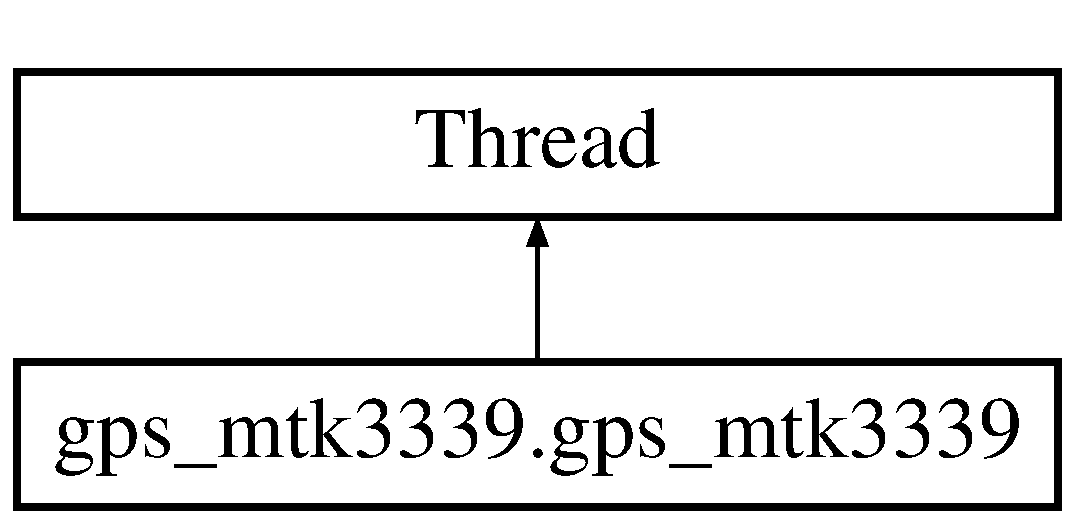
\includegraphics[height=2.000000cm]{classgps__mtk3339_1_1gps__mtk3339}
\end{center}
\end{figure}
\subsection*{Public Member Functions}
\begin{DoxyCompactItemize}
\item 
def \hyperlink{classgps__mtk3339_1_1gps__mtk3339_aef9ef03ebb7337c94b529d949fa494d4}{\+\_\+\+\_\+init\+\_\+\+\_\+} (self, \hyperlink{classgps__mtk3339_1_1gps__mtk3339_a0b660f851b889fd51697772bea5a2298}{simulate}=False)
\item 
def \hyperlink{classgps__mtk3339_1_1gps__mtk3339_a83e26207ff8028de5a6b07890e096ed0}{gpsd\+\_\+link\+\_\+init} (self)
\item 
def \hyperlink{classgps__mtk3339_1_1gps__mtk3339_a9866902bcd93e9087afc6b0a2a8eb579}{restart\+\_\+gpsd} (self)
\item 
def \hyperlink{classgps__mtk3339_1_1gps__mtk3339_a9d8c94a9453d19e4aa38d44b5b29d7a1}{run} (self)
\item 
def \hyperlink{classgps__mtk3339_1_1gps__mtk3339_a39164ba4a6f8f2456e2e6a0e8ce1cb43}{process\+\_\+gps} (self)
\item 
def \hyperlink{classgps__mtk3339_1_1gps__mtk3339_a5607ce090bf92bfae717d67b0052b5bd}{reset\+\_\+gps\+\_\+data} (self)
\item 
def \hyperlink{classgps__mtk3339_1_1gps__mtk3339_a393b083e3204be987c42bd9ba2d467b9}{get\+\_\+data} (self)
\item 
def \hyperlink{classgps__mtk3339_1_1gps__mtk3339_a5dc9478c99bcdc50e5584d202d141659}{\+\_\+\+\_\+del\+\_\+\+\_\+} (self)
\item 
def \hyperlink{classgps__mtk3339_1_1gps__mtk3339_ae2ed581bc519d827d6bcee53f5edd14a}{stop} (self)
\item 
def \hyperlink{classgps__mtk3339_1_1gps__mtk3339_ad86557ad5e6c12c8336e4eda66843f25}{set\+\_\+system\+\_\+time} (self)
\end{DoxyCompactItemize}
\subsection*{Public Attributes}
\begin{DoxyCompactItemize}
\item 
\hyperlink{classgps__mtk3339_1_1gps__mtk3339_a93b7dfcb873983c3b9954afd741bb0aa}{l}
\item 
\hyperlink{classgps__mtk3339_1_1gps__mtk3339_a0b660f851b889fd51697772bea5a2298}{simulate}
\item 
\hyperlink{classgps__mtk3339_1_1gps__mtk3339_a988087d2eb3d19966849c601052fb030}{restart\+\_\+gps}
\item 
\hyperlink{classgps__mtk3339_1_1gps__mtk3339_a3dda95763250fe6d040fc99f983aa525}{present}
\item 
\hyperlink{classgps__mtk3339_1_1gps__mtk3339_a6d478bb42c50a33dbf6b3237db07f60f}{set\+\_\+time}
\item 
\hyperlink{classgps__mtk3339_1_1gps__mtk3339_a0c092f05378b720b0b426d80f42456e3}{time\+\_\+adjustment\+\_\+delta}
\item 
\hyperlink{classgps__mtk3339_1_1gps__mtk3339_a4446b75d60332e06ac86e47117c2b5c7}{data}
\item 
\hyperlink{classgps__mtk3339_1_1gps__mtk3339_a1e3e0382d54d662346c6ce131a3a7a1c}{running}
\item 
\hyperlink{classgps__mtk3339_1_1gps__mtk3339_ae1aa1ac46a38d83b9a0147401ee82b9d}{latitude}
\item 
\hyperlink{classgps__mtk3339_1_1gps__mtk3339_a8cec49a353d5c9841d744619010be747}{longitude}
\item 
\hyperlink{classgps__mtk3339_1_1gps__mtk3339_aa7849c72105267400545a92f8bebc5a4}{utc}
\item 
\hyperlink{classgps__mtk3339_1_1gps__mtk3339_a1553a20b53503d886d324a85090f8eae}{climb\+\_\+gps}
\item 
\hyperlink{classgps__mtk3339_1_1gps__mtk3339_ad95b0301903fcc226e36d058c8849a65}{speed\+\_\+gps}
\item 
\hyperlink{classgps__mtk3339_1_1gps__mtk3339_a741b7970706c13f0128d33293e5ea1ca}{altitude\+\_\+gps}
\item 
\hyperlink{classgps__mtk3339_1_1gps__mtk3339_a5fa5839836a0c4bb31d29e6c1efe4264}{satellites}
\item 
\hyperlink{classgps__mtk3339_1_1gps__mtk3339_a9e594b0808ce07f48847a6ce4e3ebb32}{satellitesused}
\item 
\hyperlink{classgps__mtk3339_1_1gps__mtk3339_a21c1e61f981fb2ae8ef32890bac4c89d}{fix\+\_\+mode\+\_\+gps}
\item 
\hyperlink{classgps__mtk3339_1_1gps__mtk3339_a05d58c10be98511bb26422b037f88c84}{fix\+\_\+time\+\_\+gps}
\item 
\hyperlink{classgps__mtk3339_1_1gps__mtk3339_a6e35fca669effcbdedeaec3c4767dddc}{track\+\_\+gps}
\item 
\hyperlink{classgps__mtk3339_1_1gps__mtk3339_a9a2bb8e7c1cfc87bec2f26521acdf093}{eps}
\item 
\hyperlink{classgps__mtk3339_1_1gps__mtk3339_aad9f939ba52d3f70339275d1773a74fa}{epx}
\item 
\hyperlink{classgps__mtk3339_1_1gps__mtk3339_a81312e77abb16d7241b40d64173703aa}{epv}
\item 
\hyperlink{classgps__mtk3339_1_1gps__mtk3339_a4821ad999987d73199ca687497d109ce}{ept}
\item 
\hyperlink{classgps__mtk3339_1_1gps__mtk3339_a20597647b6fc2da5e4a7d80274006714}{fix\+\_\+time}
\end{DoxyCompactItemize}


\subsection{Constructor \& Destructor Documentation}
\mbox{\Hypertarget{classgps__mtk3339_1_1gps__mtk3339_aef9ef03ebb7337c94b529d949fa494d4}\label{classgps__mtk3339_1_1gps__mtk3339_aef9ef03ebb7337c94b529d949fa494d4}} 
\index{gps\+\_\+mtk3339\+::gps\+\_\+mtk3339@{gps\+\_\+mtk3339\+::gps\+\_\+mtk3339}!\+\_\+\+\_\+init\+\_\+\+\_\+@{\+\_\+\+\_\+init\+\_\+\+\_\+}}
\index{\+\_\+\+\_\+init\+\_\+\+\_\+@{\+\_\+\+\_\+init\+\_\+\+\_\+}!gps\+\_\+mtk3339\+::gps\+\_\+mtk3339@{gps\+\_\+mtk3339\+::gps\+\_\+mtk3339}}
\subsubsection{\texorpdfstring{\+\_\+\+\_\+init\+\_\+\+\_\+()}{\_\_init\_\_()}}
{\footnotesize\ttfamily def gps\+\_\+mtk3339.\+gps\+\_\+mtk3339.\+\_\+\+\_\+init\+\_\+\+\_\+ (\begin{DoxyParamCaption}\item[{}]{self,  }\item[{}]{simulate = {\ttfamily False} }\end{DoxyParamCaption})}

\mbox{\Hypertarget{classgps__mtk3339_1_1gps__mtk3339_a5dc9478c99bcdc50e5584d202d141659}\label{classgps__mtk3339_1_1gps__mtk3339_a5dc9478c99bcdc50e5584d202d141659}} 
\index{gps\+\_\+mtk3339\+::gps\+\_\+mtk3339@{gps\+\_\+mtk3339\+::gps\+\_\+mtk3339}!\+\_\+\+\_\+del\+\_\+\+\_\+@{\+\_\+\+\_\+del\+\_\+\+\_\+}}
\index{\+\_\+\+\_\+del\+\_\+\+\_\+@{\+\_\+\+\_\+del\+\_\+\+\_\+}!gps\+\_\+mtk3339\+::gps\+\_\+mtk3339@{gps\+\_\+mtk3339\+::gps\+\_\+mtk3339}}
\subsubsection{\texorpdfstring{\+\_\+\+\_\+del\+\_\+\+\_\+()}{\_\_del\_\_()}}
{\footnotesize\ttfamily def gps\+\_\+mtk3339.\+gps\+\_\+mtk3339.\+\_\+\+\_\+del\+\_\+\+\_\+ (\begin{DoxyParamCaption}\item[{}]{self }\end{DoxyParamCaption})}



\subsection{Member Function Documentation}
\mbox{\Hypertarget{classgps__mtk3339_1_1gps__mtk3339_a393b083e3204be987c42bd9ba2d467b9}\label{classgps__mtk3339_1_1gps__mtk3339_a393b083e3204be987c42bd9ba2d467b9}} 
\index{gps\+\_\+mtk3339\+::gps\+\_\+mtk3339@{gps\+\_\+mtk3339\+::gps\+\_\+mtk3339}!get\+\_\+data@{get\+\_\+data}}
\index{get\+\_\+data@{get\+\_\+data}!gps\+\_\+mtk3339\+::gps\+\_\+mtk3339@{gps\+\_\+mtk3339\+::gps\+\_\+mtk3339}}
\subsubsection{\texorpdfstring{get\+\_\+data()}{get\_data()}}
{\footnotesize\ttfamily def gps\+\_\+mtk3339.\+gps\+\_\+mtk3339.\+get\+\_\+data (\begin{DoxyParamCaption}\item[{}]{self }\end{DoxyParamCaption})}

\mbox{\Hypertarget{classgps__mtk3339_1_1gps__mtk3339_a83e26207ff8028de5a6b07890e096ed0}\label{classgps__mtk3339_1_1gps__mtk3339_a83e26207ff8028de5a6b07890e096ed0}} 
\index{gps\+\_\+mtk3339\+::gps\+\_\+mtk3339@{gps\+\_\+mtk3339\+::gps\+\_\+mtk3339}!gpsd\+\_\+link\+\_\+init@{gpsd\+\_\+link\+\_\+init}}
\index{gpsd\+\_\+link\+\_\+init@{gpsd\+\_\+link\+\_\+init}!gps\+\_\+mtk3339\+::gps\+\_\+mtk3339@{gps\+\_\+mtk3339\+::gps\+\_\+mtk3339}}
\subsubsection{\texorpdfstring{gpsd\+\_\+link\+\_\+init()}{gpsd\_link\_init()}}
{\footnotesize\ttfamily def gps\+\_\+mtk3339.\+gps\+\_\+mtk3339.\+gpsd\+\_\+link\+\_\+init (\begin{DoxyParamCaption}\item[{}]{self }\end{DoxyParamCaption})}

\mbox{\Hypertarget{classgps__mtk3339_1_1gps__mtk3339_a39164ba4a6f8f2456e2e6a0e8ce1cb43}\label{classgps__mtk3339_1_1gps__mtk3339_a39164ba4a6f8f2456e2e6a0e8ce1cb43}} 
\index{gps\+\_\+mtk3339\+::gps\+\_\+mtk3339@{gps\+\_\+mtk3339\+::gps\+\_\+mtk3339}!process\+\_\+gps@{process\+\_\+gps}}
\index{process\+\_\+gps@{process\+\_\+gps}!gps\+\_\+mtk3339\+::gps\+\_\+mtk3339@{gps\+\_\+mtk3339\+::gps\+\_\+mtk3339}}
\subsubsection{\texorpdfstring{process\+\_\+gps()}{process\_gps()}}
{\footnotesize\ttfamily def gps\+\_\+mtk3339.\+gps\+\_\+mtk3339.\+process\+\_\+gps (\begin{DoxyParamCaption}\item[{}]{self }\end{DoxyParamCaption})}

\mbox{\Hypertarget{classgps__mtk3339_1_1gps__mtk3339_a5607ce090bf92bfae717d67b0052b5bd}\label{classgps__mtk3339_1_1gps__mtk3339_a5607ce090bf92bfae717d67b0052b5bd}} 
\index{gps\+\_\+mtk3339\+::gps\+\_\+mtk3339@{gps\+\_\+mtk3339\+::gps\+\_\+mtk3339}!reset\+\_\+gps\+\_\+data@{reset\+\_\+gps\+\_\+data}}
\index{reset\+\_\+gps\+\_\+data@{reset\+\_\+gps\+\_\+data}!gps\+\_\+mtk3339\+::gps\+\_\+mtk3339@{gps\+\_\+mtk3339\+::gps\+\_\+mtk3339}}
\subsubsection{\texorpdfstring{reset\+\_\+gps\+\_\+data()}{reset\_gps\_data()}}
{\footnotesize\ttfamily def gps\+\_\+mtk3339.\+gps\+\_\+mtk3339.\+reset\+\_\+gps\+\_\+data (\begin{DoxyParamCaption}\item[{}]{self }\end{DoxyParamCaption})}

\mbox{\Hypertarget{classgps__mtk3339_1_1gps__mtk3339_a9866902bcd93e9087afc6b0a2a8eb579}\label{classgps__mtk3339_1_1gps__mtk3339_a9866902bcd93e9087afc6b0a2a8eb579}} 
\index{gps\+\_\+mtk3339\+::gps\+\_\+mtk3339@{gps\+\_\+mtk3339\+::gps\+\_\+mtk3339}!restart\+\_\+gpsd@{restart\+\_\+gpsd}}
\index{restart\+\_\+gpsd@{restart\+\_\+gpsd}!gps\+\_\+mtk3339\+::gps\+\_\+mtk3339@{gps\+\_\+mtk3339\+::gps\+\_\+mtk3339}}
\subsubsection{\texorpdfstring{restart\+\_\+gpsd()}{restart\_gpsd()}}
{\footnotesize\ttfamily def gps\+\_\+mtk3339.\+gps\+\_\+mtk3339.\+restart\+\_\+gpsd (\begin{DoxyParamCaption}\item[{}]{self }\end{DoxyParamCaption})}

\mbox{\Hypertarget{classgps__mtk3339_1_1gps__mtk3339_a9d8c94a9453d19e4aa38d44b5b29d7a1}\label{classgps__mtk3339_1_1gps__mtk3339_a9d8c94a9453d19e4aa38d44b5b29d7a1}} 
\index{gps\+\_\+mtk3339\+::gps\+\_\+mtk3339@{gps\+\_\+mtk3339\+::gps\+\_\+mtk3339}!run@{run}}
\index{run@{run}!gps\+\_\+mtk3339\+::gps\+\_\+mtk3339@{gps\+\_\+mtk3339\+::gps\+\_\+mtk3339}}
\subsubsection{\texorpdfstring{run()}{run()}}
{\footnotesize\ttfamily def gps\+\_\+mtk3339.\+gps\+\_\+mtk3339.\+run (\begin{DoxyParamCaption}\item[{}]{self }\end{DoxyParamCaption})}

\mbox{\Hypertarget{classgps__mtk3339_1_1gps__mtk3339_ad86557ad5e6c12c8336e4eda66843f25}\label{classgps__mtk3339_1_1gps__mtk3339_ad86557ad5e6c12c8336e4eda66843f25}} 
\index{gps\+\_\+mtk3339\+::gps\+\_\+mtk3339@{gps\+\_\+mtk3339\+::gps\+\_\+mtk3339}!set\+\_\+system\+\_\+time@{set\+\_\+system\+\_\+time}}
\index{set\+\_\+system\+\_\+time@{set\+\_\+system\+\_\+time}!gps\+\_\+mtk3339\+::gps\+\_\+mtk3339@{gps\+\_\+mtk3339\+::gps\+\_\+mtk3339}}
\subsubsection{\texorpdfstring{set\+\_\+system\+\_\+time()}{set\_system\_time()}}
{\footnotesize\ttfamily def gps\+\_\+mtk3339.\+gps\+\_\+mtk3339.\+set\+\_\+system\+\_\+time (\begin{DoxyParamCaption}\item[{}]{self }\end{DoxyParamCaption})}

\mbox{\Hypertarget{classgps__mtk3339_1_1gps__mtk3339_ae2ed581bc519d827d6bcee53f5edd14a}\label{classgps__mtk3339_1_1gps__mtk3339_ae2ed581bc519d827d6bcee53f5edd14a}} 
\index{gps\+\_\+mtk3339\+::gps\+\_\+mtk3339@{gps\+\_\+mtk3339\+::gps\+\_\+mtk3339}!stop@{stop}}
\index{stop@{stop}!gps\+\_\+mtk3339\+::gps\+\_\+mtk3339@{gps\+\_\+mtk3339\+::gps\+\_\+mtk3339}}
\subsubsection{\texorpdfstring{stop()}{stop()}}
{\footnotesize\ttfamily def gps\+\_\+mtk3339.\+gps\+\_\+mtk3339.\+stop (\begin{DoxyParamCaption}\item[{}]{self }\end{DoxyParamCaption})}



\subsection{Member Data Documentation}
\mbox{\Hypertarget{classgps__mtk3339_1_1gps__mtk3339_a741b7970706c13f0128d33293e5ea1ca}\label{classgps__mtk3339_1_1gps__mtk3339_a741b7970706c13f0128d33293e5ea1ca}} 
\index{gps\+\_\+mtk3339\+::gps\+\_\+mtk3339@{gps\+\_\+mtk3339\+::gps\+\_\+mtk3339}!altitude\+\_\+gps@{altitude\+\_\+gps}}
\index{altitude\+\_\+gps@{altitude\+\_\+gps}!gps\+\_\+mtk3339\+::gps\+\_\+mtk3339@{gps\+\_\+mtk3339\+::gps\+\_\+mtk3339}}
\subsubsection{\texorpdfstring{altitude\+\_\+gps}{altitude\_gps}}
{\footnotesize\ttfamily gps\+\_\+mtk3339.\+gps\+\_\+mtk3339.\+altitude\+\_\+gps}

\mbox{\Hypertarget{classgps__mtk3339_1_1gps__mtk3339_a1553a20b53503d886d324a85090f8eae}\label{classgps__mtk3339_1_1gps__mtk3339_a1553a20b53503d886d324a85090f8eae}} 
\index{gps\+\_\+mtk3339\+::gps\+\_\+mtk3339@{gps\+\_\+mtk3339\+::gps\+\_\+mtk3339}!climb\+\_\+gps@{climb\+\_\+gps}}
\index{climb\+\_\+gps@{climb\+\_\+gps}!gps\+\_\+mtk3339\+::gps\+\_\+mtk3339@{gps\+\_\+mtk3339\+::gps\+\_\+mtk3339}}
\subsubsection{\texorpdfstring{climb\+\_\+gps}{climb\_gps}}
{\footnotesize\ttfamily gps\+\_\+mtk3339.\+gps\+\_\+mtk3339.\+climb\+\_\+gps}

\mbox{\Hypertarget{classgps__mtk3339_1_1gps__mtk3339_a4446b75d60332e06ac86e47117c2b5c7}\label{classgps__mtk3339_1_1gps__mtk3339_a4446b75d60332e06ac86e47117c2b5c7}} 
\index{gps\+\_\+mtk3339\+::gps\+\_\+mtk3339@{gps\+\_\+mtk3339\+::gps\+\_\+mtk3339}!data@{data}}
\index{data@{data}!gps\+\_\+mtk3339\+::gps\+\_\+mtk3339@{gps\+\_\+mtk3339\+::gps\+\_\+mtk3339}}
\subsubsection{\texorpdfstring{data}{data}}
{\footnotesize\ttfamily gps\+\_\+mtk3339.\+gps\+\_\+mtk3339.\+data}

\mbox{\Hypertarget{classgps__mtk3339_1_1gps__mtk3339_a9a2bb8e7c1cfc87bec2f26521acdf093}\label{classgps__mtk3339_1_1gps__mtk3339_a9a2bb8e7c1cfc87bec2f26521acdf093}} 
\index{gps\+\_\+mtk3339\+::gps\+\_\+mtk3339@{gps\+\_\+mtk3339\+::gps\+\_\+mtk3339}!eps@{eps}}
\index{eps@{eps}!gps\+\_\+mtk3339\+::gps\+\_\+mtk3339@{gps\+\_\+mtk3339\+::gps\+\_\+mtk3339}}
\subsubsection{\texorpdfstring{eps}{eps}}
{\footnotesize\ttfamily gps\+\_\+mtk3339.\+gps\+\_\+mtk3339.\+eps}

\mbox{\Hypertarget{classgps__mtk3339_1_1gps__mtk3339_a4821ad999987d73199ca687497d109ce}\label{classgps__mtk3339_1_1gps__mtk3339_a4821ad999987d73199ca687497d109ce}} 
\index{gps\+\_\+mtk3339\+::gps\+\_\+mtk3339@{gps\+\_\+mtk3339\+::gps\+\_\+mtk3339}!ept@{ept}}
\index{ept@{ept}!gps\+\_\+mtk3339\+::gps\+\_\+mtk3339@{gps\+\_\+mtk3339\+::gps\+\_\+mtk3339}}
\subsubsection{\texorpdfstring{ept}{ept}}
{\footnotesize\ttfamily gps\+\_\+mtk3339.\+gps\+\_\+mtk3339.\+ept}

\mbox{\Hypertarget{classgps__mtk3339_1_1gps__mtk3339_a81312e77abb16d7241b40d64173703aa}\label{classgps__mtk3339_1_1gps__mtk3339_a81312e77abb16d7241b40d64173703aa}} 
\index{gps\+\_\+mtk3339\+::gps\+\_\+mtk3339@{gps\+\_\+mtk3339\+::gps\+\_\+mtk3339}!epv@{epv}}
\index{epv@{epv}!gps\+\_\+mtk3339\+::gps\+\_\+mtk3339@{gps\+\_\+mtk3339\+::gps\+\_\+mtk3339}}
\subsubsection{\texorpdfstring{epv}{epv}}
{\footnotesize\ttfamily gps\+\_\+mtk3339.\+gps\+\_\+mtk3339.\+epv}

\mbox{\Hypertarget{classgps__mtk3339_1_1gps__mtk3339_aad9f939ba52d3f70339275d1773a74fa}\label{classgps__mtk3339_1_1gps__mtk3339_aad9f939ba52d3f70339275d1773a74fa}} 
\index{gps\+\_\+mtk3339\+::gps\+\_\+mtk3339@{gps\+\_\+mtk3339\+::gps\+\_\+mtk3339}!epx@{epx}}
\index{epx@{epx}!gps\+\_\+mtk3339\+::gps\+\_\+mtk3339@{gps\+\_\+mtk3339\+::gps\+\_\+mtk3339}}
\subsubsection{\texorpdfstring{epx}{epx}}
{\footnotesize\ttfamily gps\+\_\+mtk3339.\+gps\+\_\+mtk3339.\+epx}

\mbox{\Hypertarget{classgps__mtk3339_1_1gps__mtk3339_a21c1e61f981fb2ae8ef32890bac4c89d}\label{classgps__mtk3339_1_1gps__mtk3339_a21c1e61f981fb2ae8ef32890bac4c89d}} 
\index{gps\+\_\+mtk3339\+::gps\+\_\+mtk3339@{gps\+\_\+mtk3339\+::gps\+\_\+mtk3339}!fix\+\_\+mode\+\_\+gps@{fix\+\_\+mode\+\_\+gps}}
\index{fix\+\_\+mode\+\_\+gps@{fix\+\_\+mode\+\_\+gps}!gps\+\_\+mtk3339\+::gps\+\_\+mtk3339@{gps\+\_\+mtk3339\+::gps\+\_\+mtk3339}}
\subsubsection{\texorpdfstring{fix\+\_\+mode\+\_\+gps}{fix\_mode\_gps}}
{\footnotesize\ttfamily gps\+\_\+mtk3339.\+gps\+\_\+mtk3339.\+fix\+\_\+mode\+\_\+gps}

\mbox{\Hypertarget{classgps__mtk3339_1_1gps__mtk3339_a20597647b6fc2da5e4a7d80274006714}\label{classgps__mtk3339_1_1gps__mtk3339_a20597647b6fc2da5e4a7d80274006714}} 
\index{gps\+\_\+mtk3339\+::gps\+\_\+mtk3339@{gps\+\_\+mtk3339\+::gps\+\_\+mtk3339}!fix\+\_\+time@{fix\+\_\+time}}
\index{fix\+\_\+time@{fix\+\_\+time}!gps\+\_\+mtk3339\+::gps\+\_\+mtk3339@{gps\+\_\+mtk3339\+::gps\+\_\+mtk3339}}
\subsubsection{\texorpdfstring{fix\+\_\+time}{fix\_time}}
{\footnotesize\ttfamily gps\+\_\+mtk3339.\+gps\+\_\+mtk3339.\+fix\+\_\+time}

\mbox{\Hypertarget{classgps__mtk3339_1_1gps__mtk3339_a05d58c10be98511bb26422b037f88c84}\label{classgps__mtk3339_1_1gps__mtk3339_a05d58c10be98511bb26422b037f88c84}} 
\index{gps\+\_\+mtk3339\+::gps\+\_\+mtk3339@{gps\+\_\+mtk3339\+::gps\+\_\+mtk3339}!fix\+\_\+time\+\_\+gps@{fix\+\_\+time\+\_\+gps}}
\index{fix\+\_\+time\+\_\+gps@{fix\+\_\+time\+\_\+gps}!gps\+\_\+mtk3339\+::gps\+\_\+mtk3339@{gps\+\_\+mtk3339\+::gps\+\_\+mtk3339}}
\subsubsection{\texorpdfstring{fix\+\_\+time\+\_\+gps}{fix\_time\_gps}}
{\footnotesize\ttfamily gps\+\_\+mtk3339.\+gps\+\_\+mtk3339.\+fix\+\_\+time\+\_\+gps}

\mbox{\Hypertarget{classgps__mtk3339_1_1gps__mtk3339_a93b7dfcb873983c3b9954afd741bb0aa}\label{classgps__mtk3339_1_1gps__mtk3339_a93b7dfcb873983c3b9954afd741bb0aa}} 
\index{gps\+\_\+mtk3339\+::gps\+\_\+mtk3339@{gps\+\_\+mtk3339\+::gps\+\_\+mtk3339}!l@{l}}
\index{l@{l}!gps\+\_\+mtk3339\+::gps\+\_\+mtk3339@{gps\+\_\+mtk3339\+::gps\+\_\+mtk3339}}
\subsubsection{\texorpdfstring{l}{l}}
{\footnotesize\ttfamily gps\+\_\+mtk3339.\+gps\+\_\+mtk3339.\+l}

\mbox{\Hypertarget{classgps__mtk3339_1_1gps__mtk3339_ae1aa1ac46a38d83b9a0147401ee82b9d}\label{classgps__mtk3339_1_1gps__mtk3339_ae1aa1ac46a38d83b9a0147401ee82b9d}} 
\index{gps\+\_\+mtk3339\+::gps\+\_\+mtk3339@{gps\+\_\+mtk3339\+::gps\+\_\+mtk3339}!latitude@{latitude}}
\index{latitude@{latitude}!gps\+\_\+mtk3339\+::gps\+\_\+mtk3339@{gps\+\_\+mtk3339\+::gps\+\_\+mtk3339}}
\subsubsection{\texorpdfstring{latitude}{latitude}}
{\footnotesize\ttfamily gps\+\_\+mtk3339.\+gps\+\_\+mtk3339.\+latitude}

\mbox{\Hypertarget{classgps__mtk3339_1_1gps__mtk3339_a8cec49a353d5c9841d744619010be747}\label{classgps__mtk3339_1_1gps__mtk3339_a8cec49a353d5c9841d744619010be747}} 
\index{gps\+\_\+mtk3339\+::gps\+\_\+mtk3339@{gps\+\_\+mtk3339\+::gps\+\_\+mtk3339}!longitude@{longitude}}
\index{longitude@{longitude}!gps\+\_\+mtk3339\+::gps\+\_\+mtk3339@{gps\+\_\+mtk3339\+::gps\+\_\+mtk3339}}
\subsubsection{\texorpdfstring{longitude}{longitude}}
{\footnotesize\ttfamily gps\+\_\+mtk3339.\+gps\+\_\+mtk3339.\+longitude}

\mbox{\Hypertarget{classgps__mtk3339_1_1gps__mtk3339_a3dda95763250fe6d040fc99f983aa525}\label{classgps__mtk3339_1_1gps__mtk3339_a3dda95763250fe6d040fc99f983aa525}} 
\index{gps\+\_\+mtk3339\+::gps\+\_\+mtk3339@{gps\+\_\+mtk3339\+::gps\+\_\+mtk3339}!present@{present}}
\index{present@{present}!gps\+\_\+mtk3339\+::gps\+\_\+mtk3339@{gps\+\_\+mtk3339\+::gps\+\_\+mtk3339}}
\subsubsection{\texorpdfstring{present}{present}}
{\footnotesize\ttfamily gps\+\_\+mtk3339.\+gps\+\_\+mtk3339.\+present}

\mbox{\Hypertarget{classgps__mtk3339_1_1gps__mtk3339_a988087d2eb3d19966849c601052fb030}\label{classgps__mtk3339_1_1gps__mtk3339_a988087d2eb3d19966849c601052fb030}} 
\index{gps\+\_\+mtk3339\+::gps\+\_\+mtk3339@{gps\+\_\+mtk3339\+::gps\+\_\+mtk3339}!restart\+\_\+gps@{restart\+\_\+gps}}
\index{restart\+\_\+gps@{restart\+\_\+gps}!gps\+\_\+mtk3339\+::gps\+\_\+mtk3339@{gps\+\_\+mtk3339\+::gps\+\_\+mtk3339}}
\subsubsection{\texorpdfstring{restart\+\_\+gps}{restart\_gps}}
{\footnotesize\ttfamily gps\+\_\+mtk3339.\+gps\+\_\+mtk3339.\+restart\+\_\+gps}

\mbox{\Hypertarget{classgps__mtk3339_1_1gps__mtk3339_a1e3e0382d54d662346c6ce131a3a7a1c}\label{classgps__mtk3339_1_1gps__mtk3339_a1e3e0382d54d662346c6ce131a3a7a1c}} 
\index{gps\+\_\+mtk3339\+::gps\+\_\+mtk3339@{gps\+\_\+mtk3339\+::gps\+\_\+mtk3339}!running@{running}}
\index{running@{running}!gps\+\_\+mtk3339\+::gps\+\_\+mtk3339@{gps\+\_\+mtk3339\+::gps\+\_\+mtk3339}}
\subsubsection{\texorpdfstring{running}{running}}
{\footnotesize\ttfamily gps\+\_\+mtk3339.\+gps\+\_\+mtk3339.\+running}

\mbox{\Hypertarget{classgps__mtk3339_1_1gps__mtk3339_a5fa5839836a0c4bb31d29e6c1efe4264}\label{classgps__mtk3339_1_1gps__mtk3339_a5fa5839836a0c4bb31d29e6c1efe4264}} 
\index{gps\+\_\+mtk3339\+::gps\+\_\+mtk3339@{gps\+\_\+mtk3339\+::gps\+\_\+mtk3339}!satellites@{satellites}}
\index{satellites@{satellites}!gps\+\_\+mtk3339\+::gps\+\_\+mtk3339@{gps\+\_\+mtk3339\+::gps\+\_\+mtk3339}}
\subsubsection{\texorpdfstring{satellites}{satellites}}
{\footnotesize\ttfamily gps\+\_\+mtk3339.\+gps\+\_\+mtk3339.\+satellites}

\mbox{\Hypertarget{classgps__mtk3339_1_1gps__mtk3339_a9e594b0808ce07f48847a6ce4e3ebb32}\label{classgps__mtk3339_1_1gps__mtk3339_a9e594b0808ce07f48847a6ce4e3ebb32}} 
\index{gps\+\_\+mtk3339\+::gps\+\_\+mtk3339@{gps\+\_\+mtk3339\+::gps\+\_\+mtk3339}!satellitesused@{satellitesused}}
\index{satellitesused@{satellitesused}!gps\+\_\+mtk3339\+::gps\+\_\+mtk3339@{gps\+\_\+mtk3339\+::gps\+\_\+mtk3339}}
\subsubsection{\texorpdfstring{satellitesused}{satellitesused}}
{\footnotesize\ttfamily gps\+\_\+mtk3339.\+gps\+\_\+mtk3339.\+satellitesused}

\mbox{\Hypertarget{classgps__mtk3339_1_1gps__mtk3339_a6d478bb42c50a33dbf6b3237db07f60f}\label{classgps__mtk3339_1_1gps__mtk3339_a6d478bb42c50a33dbf6b3237db07f60f}} 
\index{gps\+\_\+mtk3339\+::gps\+\_\+mtk3339@{gps\+\_\+mtk3339\+::gps\+\_\+mtk3339}!set\+\_\+time@{set\+\_\+time}}
\index{set\+\_\+time@{set\+\_\+time}!gps\+\_\+mtk3339\+::gps\+\_\+mtk3339@{gps\+\_\+mtk3339\+::gps\+\_\+mtk3339}}
\subsubsection{\texorpdfstring{set\+\_\+time}{set\_time}}
{\footnotesize\ttfamily gps\+\_\+mtk3339.\+gps\+\_\+mtk3339.\+set\+\_\+time}

\mbox{\Hypertarget{classgps__mtk3339_1_1gps__mtk3339_a0b660f851b889fd51697772bea5a2298}\label{classgps__mtk3339_1_1gps__mtk3339_a0b660f851b889fd51697772bea5a2298}} 
\index{gps\+\_\+mtk3339\+::gps\+\_\+mtk3339@{gps\+\_\+mtk3339\+::gps\+\_\+mtk3339}!simulate@{simulate}}
\index{simulate@{simulate}!gps\+\_\+mtk3339\+::gps\+\_\+mtk3339@{gps\+\_\+mtk3339\+::gps\+\_\+mtk3339}}
\subsubsection{\texorpdfstring{simulate}{simulate}}
{\footnotesize\ttfamily gps\+\_\+mtk3339.\+gps\+\_\+mtk3339.\+simulate}

\mbox{\Hypertarget{classgps__mtk3339_1_1gps__mtk3339_ad95b0301903fcc226e36d058c8849a65}\label{classgps__mtk3339_1_1gps__mtk3339_ad95b0301903fcc226e36d058c8849a65}} 
\index{gps\+\_\+mtk3339\+::gps\+\_\+mtk3339@{gps\+\_\+mtk3339\+::gps\+\_\+mtk3339}!speed\+\_\+gps@{speed\+\_\+gps}}
\index{speed\+\_\+gps@{speed\+\_\+gps}!gps\+\_\+mtk3339\+::gps\+\_\+mtk3339@{gps\+\_\+mtk3339\+::gps\+\_\+mtk3339}}
\subsubsection{\texorpdfstring{speed\+\_\+gps}{speed\_gps}}
{\footnotesize\ttfamily gps\+\_\+mtk3339.\+gps\+\_\+mtk3339.\+speed\+\_\+gps}

\mbox{\Hypertarget{classgps__mtk3339_1_1gps__mtk3339_a0c092f05378b720b0b426d80f42456e3}\label{classgps__mtk3339_1_1gps__mtk3339_a0c092f05378b720b0b426d80f42456e3}} 
\index{gps\+\_\+mtk3339\+::gps\+\_\+mtk3339@{gps\+\_\+mtk3339\+::gps\+\_\+mtk3339}!time\+\_\+adjustment\+\_\+delta@{time\+\_\+adjustment\+\_\+delta}}
\index{time\+\_\+adjustment\+\_\+delta@{time\+\_\+adjustment\+\_\+delta}!gps\+\_\+mtk3339\+::gps\+\_\+mtk3339@{gps\+\_\+mtk3339\+::gps\+\_\+mtk3339}}
\subsubsection{\texorpdfstring{time\+\_\+adjustment\+\_\+delta}{time\_adjustment\_delta}}
{\footnotesize\ttfamily gps\+\_\+mtk3339.\+gps\+\_\+mtk3339.\+time\+\_\+adjustment\+\_\+delta}

\mbox{\Hypertarget{classgps__mtk3339_1_1gps__mtk3339_a6e35fca669effcbdedeaec3c4767dddc}\label{classgps__mtk3339_1_1gps__mtk3339_a6e35fca669effcbdedeaec3c4767dddc}} 
\index{gps\+\_\+mtk3339\+::gps\+\_\+mtk3339@{gps\+\_\+mtk3339\+::gps\+\_\+mtk3339}!track\+\_\+gps@{track\+\_\+gps}}
\index{track\+\_\+gps@{track\+\_\+gps}!gps\+\_\+mtk3339\+::gps\+\_\+mtk3339@{gps\+\_\+mtk3339\+::gps\+\_\+mtk3339}}
\subsubsection{\texorpdfstring{track\+\_\+gps}{track\_gps}}
{\footnotesize\ttfamily gps\+\_\+mtk3339.\+gps\+\_\+mtk3339.\+track\+\_\+gps}

\mbox{\Hypertarget{classgps__mtk3339_1_1gps__mtk3339_aa7849c72105267400545a92f8bebc5a4}\label{classgps__mtk3339_1_1gps__mtk3339_aa7849c72105267400545a92f8bebc5a4}} 
\index{gps\+\_\+mtk3339\+::gps\+\_\+mtk3339@{gps\+\_\+mtk3339\+::gps\+\_\+mtk3339}!utc@{utc}}
\index{utc@{utc}!gps\+\_\+mtk3339\+::gps\+\_\+mtk3339@{gps\+\_\+mtk3339\+::gps\+\_\+mtk3339}}
\subsubsection{\texorpdfstring{utc}{utc}}
{\footnotesize\ttfamily gps\+\_\+mtk3339.\+gps\+\_\+mtk3339.\+utc}



The documentation for this class was generated from the following file\+:\begin{DoxyCompactItemize}
\item 
src/\hyperlink{gps__mtk3339_8py}{gps\+\_\+mtk3339.\+py}\end{DoxyCompactItemize}

\hypertarget{classble__hr_1_1HR__Delegate}{}\section{ble\+\_\+hr.\+H\+R\+\_\+\+Delegate Class Reference}
\label{classble__hr_1_1HR__Delegate}\index{ble\+\_\+hr.\+H\+R\+\_\+\+Delegate@{ble\+\_\+hr.\+H\+R\+\_\+\+Delegate}}
Inheritance diagram for ble\+\_\+hr.\+H\+R\+\_\+\+Delegate\+:\begin{figure}[H]
\begin{center}
\leavevmode
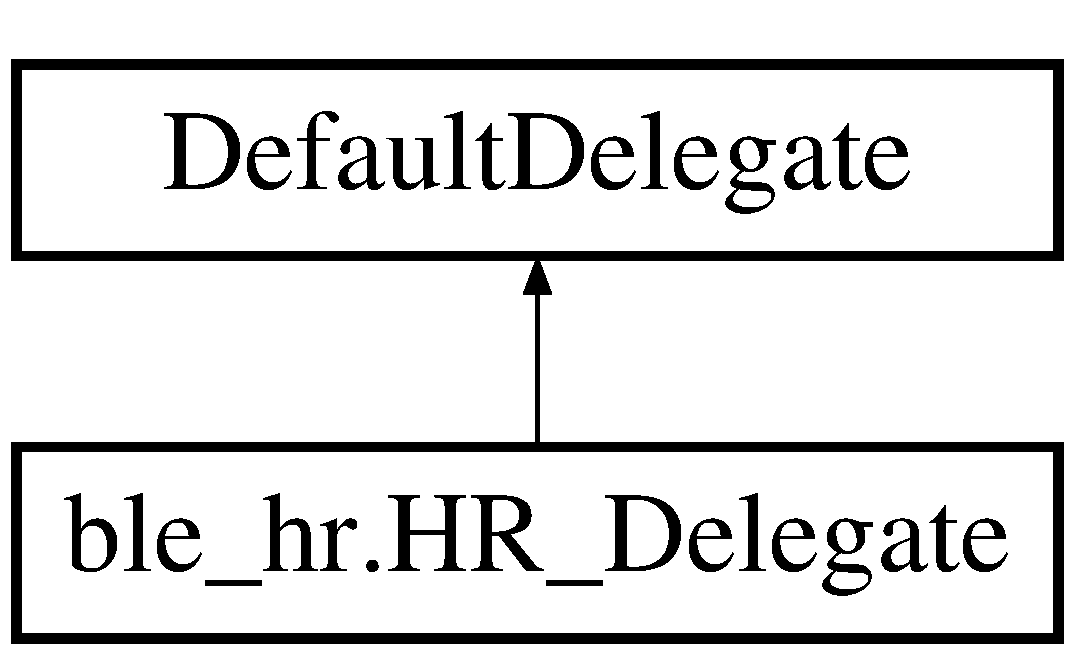
\includegraphics[height=2.000000cm]{classble__hr_1_1HR__Delegate}
\end{center}
\end{figure}
\subsection*{Public Member Functions}
\begin{DoxyCompactItemize}
\item 
def \hyperlink{classble__hr_1_1HR__Delegate_a50888fdeec27db99c92d8fcf1bf661e7}{\+\_\+\+\_\+init\+\_\+\+\_\+} (self)
\item 
def \hyperlink{classble__hr_1_1HR__Delegate_a373ab424d0357665265754d1a54ce093}{handle\+Notification} (self, c\+Handle, data)
\end{DoxyCompactItemize}
\subsection*{Public Attributes}
\begin{DoxyCompactItemize}
\item 
\hyperlink{classble__hr_1_1HR__Delegate_ad442fb90fb3f92ca843ee0c925e680e4}{l}
\item 
\hyperlink{classble__hr_1_1HR__Delegate_a54dcf43e7f403635aa14aba00626858e}{heart\+\_\+rate}
\item 
\hyperlink{classble__hr_1_1HR__Delegate_abf244fc6909adeb05d6d1e0cb549f357}{time\+\_\+stamp}
\end{DoxyCompactItemize}


\subsection{Constructor \& Destructor Documentation}
\mbox{\Hypertarget{classble__hr_1_1HR__Delegate_a50888fdeec27db99c92d8fcf1bf661e7}\label{classble__hr_1_1HR__Delegate_a50888fdeec27db99c92d8fcf1bf661e7}} 
\index{ble\+\_\+hr\+::\+H\+R\+\_\+\+Delegate@{ble\+\_\+hr\+::\+H\+R\+\_\+\+Delegate}!\+\_\+\+\_\+init\+\_\+\+\_\+@{\+\_\+\+\_\+init\+\_\+\+\_\+}}
\index{\+\_\+\+\_\+init\+\_\+\+\_\+@{\+\_\+\+\_\+init\+\_\+\+\_\+}!ble\+\_\+hr\+::\+H\+R\+\_\+\+Delegate@{ble\+\_\+hr\+::\+H\+R\+\_\+\+Delegate}}
\subsubsection{\texorpdfstring{\+\_\+\+\_\+init\+\_\+\+\_\+()}{\_\_init\_\_()}}
{\footnotesize\ttfamily def ble\+\_\+hr.\+H\+R\+\_\+\+Delegate.\+\_\+\+\_\+init\+\_\+\+\_\+ (\begin{DoxyParamCaption}\item[{}]{self }\end{DoxyParamCaption})}



\subsection{Member Function Documentation}
\mbox{\Hypertarget{classble__hr_1_1HR__Delegate_a373ab424d0357665265754d1a54ce093}\label{classble__hr_1_1HR__Delegate_a373ab424d0357665265754d1a54ce093}} 
\index{ble\+\_\+hr\+::\+H\+R\+\_\+\+Delegate@{ble\+\_\+hr\+::\+H\+R\+\_\+\+Delegate}!handle\+Notification@{handle\+Notification}}
\index{handle\+Notification@{handle\+Notification}!ble\+\_\+hr\+::\+H\+R\+\_\+\+Delegate@{ble\+\_\+hr\+::\+H\+R\+\_\+\+Delegate}}
\subsubsection{\texorpdfstring{handle\+Notification()}{handleNotification()}}
{\footnotesize\ttfamily def ble\+\_\+hr.\+H\+R\+\_\+\+Delegate.\+handle\+Notification (\begin{DoxyParamCaption}\item[{}]{self,  }\item[{}]{c\+Handle,  }\item[{}]{data }\end{DoxyParamCaption})}



\subsection{Member Data Documentation}
\mbox{\Hypertarget{classble__hr_1_1HR__Delegate_a54dcf43e7f403635aa14aba00626858e}\label{classble__hr_1_1HR__Delegate_a54dcf43e7f403635aa14aba00626858e}} 
\index{ble\+\_\+hr\+::\+H\+R\+\_\+\+Delegate@{ble\+\_\+hr\+::\+H\+R\+\_\+\+Delegate}!heart\+\_\+rate@{heart\+\_\+rate}}
\index{heart\+\_\+rate@{heart\+\_\+rate}!ble\+\_\+hr\+::\+H\+R\+\_\+\+Delegate@{ble\+\_\+hr\+::\+H\+R\+\_\+\+Delegate}}
\subsubsection{\texorpdfstring{heart\+\_\+rate}{heart\_rate}}
{\footnotesize\ttfamily ble\+\_\+hr.\+H\+R\+\_\+\+Delegate.\+heart\+\_\+rate}

\mbox{\Hypertarget{classble__hr_1_1HR__Delegate_ad442fb90fb3f92ca843ee0c925e680e4}\label{classble__hr_1_1HR__Delegate_ad442fb90fb3f92ca843ee0c925e680e4}} 
\index{ble\+\_\+hr\+::\+H\+R\+\_\+\+Delegate@{ble\+\_\+hr\+::\+H\+R\+\_\+\+Delegate}!l@{l}}
\index{l@{l}!ble\+\_\+hr\+::\+H\+R\+\_\+\+Delegate@{ble\+\_\+hr\+::\+H\+R\+\_\+\+Delegate}}
\subsubsection{\texorpdfstring{l}{l}}
{\footnotesize\ttfamily ble\+\_\+hr.\+H\+R\+\_\+\+Delegate.\+l}

\mbox{\Hypertarget{classble__hr_1_1HR__Delegate_abf244fc6909adeb05d6d1e0cb549f357}\label{classble__hr_1_1HR__Delegate_abf244fc6909adeb05d6d1e0cb549f357}} 
\index{ble\+\_\+hr\+::\+H\+R\+\_\+\+Delegate@{ble\+\_\+hr\+::\+H\+R\+\_\+\+Delegate}!time\+\_\+stamp@{time\+\_\+stamp}}
\index{time\+\_\+stamp@{time\+\_\+stamp}!ble\+\_\+hr\+::\+H\+R\+\_\+\+Delegate@{ble\+\_\+hr\+::\+H\+R\+\_\+\+Delegate}}
\subsubsection{\texorpdfstring{time\+\_\+stamp}{time\_stamp}}
{\footnotesize\ttfamily ble\+\_\+hr.\+H\+R\+\_\+\+Delegate.\+time\+\_\+stamp}



The documentation for this class was generated from the following file\+:\begin{DoxyCompactItemize}
\item 
src/\hyperlink{ble__hr_8py}{ble\+\_\+hr.\+py}\end{DoxyCompactItemize}

\hypertarget{classlayout_1_1layout}{}\section{layout.\+layout Class Reference}
\label{classlayout_1_1layout}\index{layout.\+layout@{layout.\+layout}}
\subsection*{Public Member Functions}
\begin{DoxyCompactItemize}
\item 
def \hyperlink{classlayout_1_1layout_a7e47cd5d1e93a4b4515b1fb8a30941ec}{\+\_\+\+\_\+init\+\_\+\+\_\+} (self, \hyperlink{classlayout_1_1layout_ac2fa1280be7977398ef3930c71568bdc}{occ}, \hyperlink{classlayout_1_1layout_ac7b9c2e760d1fd038ee8713760a5da73}{layout\+\_\+path}=\char`\"{}layouts/default.\+xml\char`\"{})
\item 
def \hyperlink{classlayout_1_1layout_a7275c3be35b52fa7b405994e2c999b83}{load\+\_\+layout} (self, \hyperlink{classlayout_1_1layout_ac7b9c2e760d1fd038ee8713760a5da73}{layout\+\_\+path})
\item 
def \hyperlink{classlayout_1_1layout_ad4a9522d6b342298ee823e66686ab124}{write\+\_\+layout} (self, \hyperlink{classlayout_1_1layout_ac7b9c2e760d1fd038ee8713760a5da73}{layout\+\_\+path}=\char`\"{}layouts/current.\+xml\char`\"{})
\item 
def \hyperlink{classlayout_1_1layout_a70d998b8441cf6d9931cb6fdfdc2309a}{ble\+\_\+scan} (self)
\item 
def \hyperlink{classlayout_1_1layout_a738271d751090e49ae0affb1439cd582}{ble\+\_\+dev\+\_\+helper} (self, no, master)
\item 
def \hyperlink{classlayout_1_1layout_a20c8e24a7a8656819e917c23d8e790d5}{ble\+\_\+dev\+\_\+name\+\_\+1} (self)
\item 
def \hyperlink{classlayout_1_1layout_a70c3e0d51b1b68f6a4a059fa66af2cb8}{ble\+\_\+dev\+\_\+name\+\_\+2} (self)
\item 
def \hyperlink{classlayout_1_1layout_a835859b89233c571315a16d4df7062f4}{ble\+\_\+dev\+\_\+name\+\_\+3} (self)
\item 
def \hyperlink{classlayout_1_1layout_a7d58e5dcfe0415b65397d085427846c7}{ble\+\_\+dev\+\_\+name\+\_\+4} (self)
\item 
def \hyperlink{classlayout_1_1layout_af9d992ec7a77a1f8975d42e474085607}{use\+\_\+page} (self, page\+\_\+id=\char`\"{}page\+\_\+0\char`\"{})
\item 
def \hyperlink{classlayout_1_1layout_a1b573b32602a66ec97122d5931ecab77}{load\+\_\+image} (self, text\+\_\+center)
\item 
def \hyperlink{classlayout_1_1layout_a915717bcd06193f482be2d3589f39d35}{use\+\_\+main\+\_\+page} (self)
\item 
def \hyperlink{classlayout_1_1layout_aa200719d593ee03ec498e80c5df237b0}{render\+\_\+background} (self, \hyperlink{classlayout_1_1layout_aa588f7b44d84ec47ee98b72d8931b32c}{screen})
\item 
def \hyperlink{classlayout_1_1layout_ae261bab4b37b3348bb40a4e2b68b7e58}{render\+\_\+pressed\+\_\+button} (self, \hyperlink{classlayout_1_1layout_aa588f7b44d84ec47ee98b72d8931b32c}{screen}, function)
\item 
def \hyperlink{classlayout_1_1layout_abd46ee3f166659e915b84683c0ffb0ec}{render\+\_\+page} (self)
\item 
def \hyperlink{classlayout_1_1layout_abc33e3886bca018ac33da77dd4665f81}{make\+\_\+image\+\_\+key} (self, image\+\_\+path, value)
\item 
def \hyperlink{classlayout_1_1layout_a338f0c3d04a721a701c3314c373a48f9}{render} (self, \hyperlink{classlayout_1_1layout_aa588f7b44d84ec47ee98b72d8931b32c}{screen})
\item 
def \hyperlink{classlayout_1_1layout_a8f9f8eb17c9a17bbc794fbef0a76a1c2}{show\+\_\+pressed\+\_\+button} (self)
\item 
def \hyperlink{classlayout_1_1layout_a1a4821d5cfdcbbc1c6bccccf3ee67039}{check\+\_\+click} (self, position, click)
\item 
def \hyperlink{classlayout_1_1layout_adfea7db87304e6bae605e923ce55c92f}{open\+\_\+editor\+\_\+page} (self, editor\+\_\+name, function)
\item 
def \hyperlink{classlayout_1_1layout_a0825882f1e0abfa53dd1d21c8eb5deba}{run\+\_\+function} (self, name)
\item 
def \hyperlink{classlayout_1_1layout_a38a02d29f24a3fe87472a4c77432b663}{force\+\_\+refresh} (self)
\item 
def \hyperlink{classlayout_1_1layout_aa098e066333cb4deb0ff6187c0295e50}{load\+\_\+page\+\_\+0} (self)
\item 
def \hyperlink{classlayout_1_1layout_a321003a72646314f4f626c37ea66fa2e}{load\+\_\+settings\+\_\+page} (self)
\item 
def \hyperlink{classlayout_1_1layout_a6bc6dd51cd0974eed07281fb63f8f293}{ed\+\_\+accept} (self)
\item 
def \hyperlink{classlayout_1_1layout_a866dcbea40c0fb70b194137fd98a6ced}{ed\+\_\+cancel} (self)
\item 
def \hyperlink{classlayout_1_1layout_a869abc577f8835970f78775496638c3a}{ed\+\_\+decrease} (self)
\item 
def \hyperlink{classlayout_1_1layout_a998414989210d42a9132236290d8e7a7}{ed\+\_\+increase} (self)
\item 
def \hyperlink{classlayout_1_1layout_a15504939ad10f87020d0910fd7374bed}{ed\+\_\+next} (self)
\item 
def \hyperlink{classlayout_1_1layout_a806ed3d52003228e1c7bcc0047287040}{ed\+\_\+prev} (self)
\item 
def \hyperlink{classlayout_1_1layout_a8d3ec5f26da1b5e2fd4587ebddd76c83}{ed\+\_\+change\+\_\+unit} (self, direction)
\item 
def \hyperlink{classlayout_1_1layout_ae0141cdca0be7dd22e9da7b2464cc317}{ed\+\_\+next\+\_\+unit} (self)
\item 
def \hyperlink{classlayout_1_1layout_a1ebfb6c0f86169a4cc4a5fce54533f9c}{ed\+\_\+prev\+\_\+unit} (self)
\item 
def \hyperlink{classlayout_1_1layout_aadca21149875e45fbb0296dd7f20e7c5}{accept\+\_\+edit} (self)
\item 
def \hyperlink{classlayout_1_1layout_afb35c9f363f82940357e512c2e8da4ce}{get\+\_\+page} (self, page\+\_\+type, page\+\_\+no)
\item 
def \hyperlink{classlayout_1_1layout_a6c2fd6be83cae3597b4ebe6f9c311217}{next\+\_\+page} (self)
\item 
def \hyperlink{classlayout_1_1layout_a2a84004ae84bcf89e33faf6fb9fd5ddc}{prev\+\_\+page} (self)
\item 
def \hyperlink{classlayout_1_1layout_a2829719adca767c425e1f6250198e2ea}{load\+\_\+layout\+\_\+by\+\_\+name} (self, name)
\item 
def \hyperlink{classlayout_1_1layout_acd974259d2135316a557ff7f4400141f}{load\+\_\+current\+\_\+layout} (self)
\item 
def \hyperlink{classlayout_1_1layout_a431f05998b17b8c26b78b40cee4ac8f0}{load\+\_\+default\+\_\+layout} (self)
\item 
def \hyperlink{classlayout_1_1layout_a919675f9c2c0b6dd9c1bd3e1310a2ab3}{quit} (self)
\item 
def \hyperlink{classlayout_1_1layout_a29b0ea3c979e6254436eb91dd4e92bc5}{reboot} (self)
\item 
def \hyperlink{classlayout_1_1layout_ab3d0775d4a7f40e99f97839bb8e04692}{halt} (self)
\item 
def \hyperlink{classlayout_1_1layout_a0f2bebab606bc3a5b8d8556efe9a3769}{debug\+\_\+level} (self)
\end{DoxyCompactItemize}
\subsection*{Public Attributes}
\begin{DoxyCompactItemize}
\item 
\hyperlink{classlayout_1_1layout_ac2fa1280be7977398ef3930c71568bdc}{occ}
\item 
\hyperlink{classlayout_1_1layout_a4e986be62085ff0ab88f24f4f053a955}{l}
\item 
\hyperlink{classlayout_1_1layout_a6e471177d664a814812f91fddef0b7d5}{uc}
\item 
\hyperlink{classlayout_1_1layout_aa588f7b44d84ec47ee98b72d8931b32c}{screen}
\item 
\hyperlink{classlayout_1_1layout_af1446e9aff89ce7dc077ffbfb712a052}{colorkey}
\item 
\hyperlink{classlayout_1_1layout_aee06a90eb791724cd6e202d6f88d31c6}{alpha}
\item 
\hyperlink{classlayout_1_1layout_a06edc6452a97f2a9d01458b4be14a667}{font\+\_\+list}
\item 
\hyperlink{classlayout_1_1layout_ac2a7dddbdc8f01532f9a0909020b2232}{page\+\_\+list}
\item 
\hyperlink{classlayout_1_1layout_a7c8c93302999f031ee770dcb10573bce}{page\+\_\+index}
\item 
\hyperlink{classlayout_1_1layout_af63f4624614b7ae46c605cd3b9d423b0}{function\+\_\+rect\+\_\+list}
\item 
\hyperlink{classlayout_1_1layout_ad5d1acad80f3953301aa65f70f60a58c}{current\+\_\+function\+\_\+list}
\item 
\hyperlink{classlayout_1_1layout_af54aa665178f598e88cb6016e8a5e708}{current\+\_\+image\+\_\+list}
\item 
\hyperlink{classlayout_1_1layout_ac7b9c2e760d1fd038ee8713760a5da73}{layout\+\_\+path}
\item 
\hyperlink{classlayout_1_1layout_a97a69f80a2dbb74741ea77e29ee120bf}{render\+\_\+button}
\item 
\hyperlink{classlayout_1_1layout_a88de9975a466f3626ca730c6e2d6f44e}{max\+\_\+page\+\_\+id}
\item 
\hyperlink{classlayout_1_1layout_a875fbf0d63aa271f27de8ae4cb877326}{max\+\_\+settings\+\_\+id}
\item 
\hyperlink{classlayout_1_1layout_ae5432ae42bbf064247b2786253de56eb}{layout\+\_\+tree}
\item 
\hyperlink{classlayout_1_1layout_a7e12699e54d9a8aeb1e0a7716c3f13ea}{pages}
\item 
\hyperlink{classlayout_1_1layout_ae264b7570332c1e7d132b454483c12de}{current\+\_\+button\+\_\+list}
\item 
\hyperlink{classlayout_1_1layout_a1da959c61cfda61d0fbb6abc02f783e0}{current\+\_\+page}
\item 
\hyperlink{classlayout_1_1layout_a97f7b2c70908a32213c7c924abb7c298}{bg\+\_\+image}
\item 
\hyperlink{classlayout_1_1layout_a95ef146e9091ffb6a616ec1905b19a7d}{bt\+\_\+image}
\item 
\hyperlink{classlayout_1_1layout_a90ef9f3feda1913b0aca58e733f23f73}{font}
\item 
\hyperlink{classlayout_1_1layout_afae5a27bb85f620ea9a9d10d0da9495d}{fg\+\_\+colour\+\_\+rgb}
\item 
\hyperlink{classlayout_1_1layout_a6d811ee392218a0f440d4ac4db94a0ed}{fg\+\_\+colour}
\end{DoxyCompactItemize}


\subsection{Constructor \& Destructor Documentation}
\mbox{\Hypertarget{classlayout_1_1layout_a7e47cd5d1e93a4b4515b1fb8a30941ec}\label{classlayout_1_1layout_a7e47cd5d1e93a4b4515b1fb8a30941ec}} 
\index{layout\+::layout@{layout\+::layout}!\+\_\+\+\_\+init\+\_\+\+\_\+@{\+\_\+\+\_\+init\+\_\+\+\_\+}}
\index{\+\_\+\+\_\+init\+\_\+\+\_\+@{\+\_\+\+\_\+init\+\_\+\+\_\+}!layout\+::layout@{layout\+::layout}}
\subsubsection{\texorpdfstring{\+\_\+\+\_\+init\+\_\+\+\_\+()}{\_\_init\_\_()}}
{\footnotesize\ttfamily def layout.\+layout.\+\_\+\+\_\+init\+\_\+\+\_\+ (\begin{DoxyParamCaption}\item[{}]{self,  }\item[{}]{occ,  }\item[{}]{layout\+\_\+path = {\ttfamily \char`\"{}layouts/default.xml\char`\"{}} }\end{DoxyParamCaption})}



\subsection{Member Function Documentation}
\mbox{\Hypertarget{classlayout_1_1layout_aadca21149875e45fbb0296dd7f20e7c5}\label{classlayout_1_1layout_aadca21149875e45fbb0296dd7f20e7c5}} 
\index{layout\+::layout@{layout\+::layout}!accept\+\_\+edit@{accept\+\_\+edit}}
\index{accept\+\_\+edit@{accept\+\_\+edit}!layout\+::layout@{layout\+::layout}}
\subsubsection{\texorpdfstring{accept\+\_\+edit()}{accept\_edit()}}
{\footnotesize\ttfamily def layout.\+layout.\+accept\+\_\+edit (\begin{DoxyParamCaption}\item[{}]{self }\end{DoxyParamCaption})}

\mbox{\Hypertarget{classlayout_1_1layout_a738271d751090e49ae0affb1439cd582}\label{classlayout_1_1layout_a738271d751090e49ae0affb1439cd582}} 
\index{layout\+::layout@{layout\+::layout}!ble\+\_\+dev\+\_\+helper@{ble\+\_\+dev\+\_\+helper}}
\index{ble\+\_\+dev\+\_\+helper@{ble\+\_\+dev\+\_\+helper}!layout\+::layout@{layout\+::layout}}
\subsubsection{\texorpdfstring{ble\+\_\+dev\+\_\+helper()}{ble\_dev\_helper()}}
{\footnotesize\ttfamily def layout.\+layout.\+ble\+\_\+dev\+\_\+helper (\begin{DoxyParamCaption}\item[{}]{self,  }\item[{}]{no,  }\item[{}]{master }\end{DoxyParamCaption})}

\mbox{\Hypertarget{classlayout_1_1layout_a20c8e24a7a8656819e917c23d8e790d5}\label{classlayout_1_1layout_a20c8e24a7a8656819e917c23d8e790d5}} 
\index{layout\+::layout@{layout\+::layout}!ble\+\_\+dev\+\_\+name\+\_\+1@{ble\+\_\+dev\+\_\+name\+\_\+1}}
\index{ble\+\_\+dev\+\_\+name\+\_\+1@{ble\+\_\+dev\+\_\+name\+\_\+1}!layout\+::layout@{layout\+::layout}}
\subsubsection{\texorpdfstring{ble\+\_\+dev\+\_\+name\+\_\+1()}{ble\_dev\_name\_1()}}
{\footnotesize\ttfamily def layout.\+layout.\+ble\+\_\+dev\+\_\+name\+\_\+1 (\begin{DoxyParamCaption}\item[{}]{self }\end{DoxyParamCaption})}

\mbox{\Hypertarget{classlayout_1_1layout_a70c3e0d51b1b68f6a4a059fa66af2cb8}\label{classlayout_1_1layout_a70c3e0d51b1b68f6a4a059fa66af2cb8}} 
\index{layout\+::layout@{layout\+::layout}!ble\+\_\+dev\+\_\+name\+\_\+2@{ble\+\_\+dev\+\_\+name\+\_\+2}}
\index{ble\+\_\+dev\+\_\+name\+\_\+2@{ble\+\_\+dev\+\_\+name\+\_\+2}!layout\+::layout@{layout\+::layout}}
\subsubsection{\texorpdfstring{ble\+\_\+dev\+\_\+name\+\_\+2()}{ble\_dev\_name\_2()}}
{\footnotesize\ttfamily def layout.\+layout.\+ble\+\_\+dev\+\_\+name\+\_\+2 (\begin{DoxyParamCaption}\item[{}]{self }\end{DoxyParamCaption})}

\mbox{\Hypertarget{classlayout_1_1layout_a835859b89233c571315a16d4df7062f4}\label{classlayout_1_1layout_a835859b89233c571315a16d4df7062f4}} 
\index{layout\+::layout@{layout\+::layout}!ble\+\_\+dev\+\_\+name\+\_\+3@{ble\+\_\+dev\+\_\+name\+\_\+3}}
\index{ble\+\_\+dev\+\_\+name\+\_\+3@{ble\+\_\+dev\+\_\+name\+\_\+3}!layout\+::layout@{layout\+::layout}}
\subsubsection{\texorpdfstring{ble\+\_\+dev\+\_\+name\+\_\+3()}{ble\_dev\_name\_3()}}
{\footnotesize\ttfamily def layout.\+layout.\+ble\+\_\+dev\+\_\+name\+\_\+3 (\begin{DoxyParamCaption}\item[{}]{self }\end{DoxyParamCaption})}

\mbox{\Hypertarget{classlayout_1_1layout_a7d58e5dcfe0415b65397d085427846c7}\label{classlayout_1_1layout_a7d58e5dcfe0415b65397d085427846c7}} 
\index{layout\+::layout@{layout\+::layout}!ble\+\_\+dev\+\_\+name\+\_\+4@{ble\+\_\+dev\+\_\+name\+\_\+4}}
\index{ble\+\_\+dev\+\_\+name\+\_\+4@{ble\+\_\+dev\+\_\+name\+\_\+4}!layout\+::layout@{layout\+::layout}}
\subsubsection{\texorpdfstring{ble\+\_\+dev\+\_\+name\+\_\+4()}{ble\_dev\_name\_4()}}
{\footnotesize\ttfamily def layout.\+layout.\+ble\+\_\+dev\+\_\+name\+\_\+4 (\begin{DoxyParamCaption}\item[{}]{self }\end{DoxyParamCaption})}

\mbox{\Hypertarget{classlayout_1_1layout_a70d998b8441cf6d9931cb6fdfdc2309a}\label{classlayout_1_1layout_a70d998b8441cf6d9931cb6fdfdc2309a}} 
\index{layout\+::layout@{layout\+::layout}!ble\+\_\+scan@{ble\+\_\+scan}}
\index{ble\+\_\+scan@{ble\+\_\+scan}!layout\+::layout@{layout\+::layout}}
\subsubsection{\texorpdfstring{ble\+\_\+scan()}{ble\_scan()}}
{\footnotesize\ttfamily def layout.\+layout.\+ble\+\_\+scan (\begin{DoxyParamCaption}\item[{}]{self }\end{DoxyParamCaption})}

\mbox{\Hypertarget{classlayout_1_1layout_a1a4821d5cfdcbbc1c6bccccf3ee67039}\label{classlayout_1_1layout_a1a4821d5cfdcbbc1c6bccccf3ee67039}} 
\index{layout\+::layout@{layout\+::layout}!check\+\_\+click@{check\+\_\+click}}
\index{check\+\_\+click@{check\+\_\+click}!layout\+::layout@{layout\+::layout}}
\subsubsection{\texorpdfstring{check\+\_\+click()}{check\_click()}}
{\footnotesize\ttfamily def layout.\+layout.\+check\+\_\+click (\begin{DoxyParamCaption}\item[{}]{self,  }\item[{}]{position,  }\item[{}]{click }\end{DoxyParamCaption})}

\mbox{\Hypertarget{classlayout_1_1layout_a0f2bebab606bc3a5b8d8556efe9a3769}\label{classlayout_1_1layout_a0f2bebab606bc3a5b8d8556efe9a3769}} 
\index{layout\+::layout@{layout\+::layout}!debug\+\_\+level@{debug\+\_\+level}}
\index{debug\+\_\+level@{debug\+\_\+level}!layout\+::layout@{layout\+::layout}}
\subsubsection{\texorpdfstring{debug\+\_\+level()}{debug\_level()}}
{\footnotesize\ttfamily def layout.\+layout.\+debug\+\_\+level (\begin{DoxyParamCaption}\item[{}]{self }\end{DoxyParamCaption})}

\mbox{\Hypertarget{classlayout_1_1layout_a6bc6dd51cd0974eed07281fb63f8f293}\label{classlayout_1_1layout_a6bc6dd51cd0974eed07281fb63f8f293}} 
\index{layout\+::layout@{layout\+::layout}!ed\+\_\+accept@{ed\+\_\+accept}}
\index{ed\+\_\+accept@{ed\+\_\+accept}!layout\+::layout@{layout\+::layout}}
\subsubsection{\texorpdfstring{ed\+\_\+accept()}{ed\_accept()}}
{\footnotesize\ttfamily def layout.\+layout.\+ed\+\_\+accept (\begin{DoxyParamCaption}\item[{}]{self }\end{DoxyParamCaption})}

\mbox{\Hypertarget{classlayout_1_1layout_a866dcbea40c0fb70b194137fd98a6ced}\label{classlayout_1_1layout_a866dcbea40c0fb70b194137fd98a6ced}} 
\index{layout\+::layout@{layout\+::layout}!ed\+\_\+cancel@{ed\+\_\+cancel}}
\index{ed\+\_\+cancel@{ed\+\_\+cancel}!layout\+::layout@{layout\+::layout}}
\subsubsection{\texorpdfstring{ed\+\_\+cancel()}{ed\_cancel()}}
{\footnotesize\ttfamily def layout.\+layout.\+ed\+\_\+cancel (\begin{DoxyParamCaption}\item[{}]{self }\end{DoxyParamCaption})}

\mbox{\Hypertarget{classlayout_1_1layout_a8d3ec5f26da1b5e2fd4587ebddd76c83}\label{classlayout_1_1layout_a8d3ec5f26da1b5e2fd4587ebddd76c83}} 
\index{layout\+::layout@{layout\+::layout}!ed\+\_\+change\+\_\+unit@{ed\+\_\+change\+\_\+unit}}
\index{ed\+\_\+change\+\_\+unit@{ed\+\_\+change\+\_\+unit}!layout\+::layout@{layout\+::layout}}
\subsubsection{\texorpdfstring{ed\+\_\+change\+\_\+unit()}{ed\_change\_unit()}}
{\footnotesize\ttfamily def layout.\+layout.\+ed\+\_\+change\+\_\+unit (\begin{DoxyParamCaption}\item[{}]{self,  }\item[{}]{direction }\end{DoxyParamCaption})}

\mbox{\Hypertarget{classlayout_1_1layout_a869abc577f8835970f78775496638c3a}\label{classlayout_1_1layout_a869abc577f8835970f78775496638c3a}} 
\index{layout\+::layout@{layout\+::layout}!ed\+\_\+decrease@{ed\+\_\+decrease}}
\index{ed\+\_\+decrease@{ed\+\_\+decrease}!layout\+::layout@{layout\+::layout}}
\subsubsection{\texorpdfstring{ed\+\_\+decrease()}{ed\_decrease()}}
{\footnotesize\ttfamily def layout.\+layout.\+ed\+\_\+decrease (\begin{DoxyParamCaption}\item[{}]{self }\end{DoxyParamCaption})}

\mbox{\Hypertarget{classlayout_1_1layout_a998414989210d42a9132236290d8e7a7}\label{classlayout_1_1layout_a998414989210d42a9132236290d8e7a7}} 
\index{layout\+::layout@{layout\+::layout}!ed\+\_\+increase@{ed\+\_\+increase}}
\index{ed\+\_\+increase@{ed\+\_\+increase}!layout\+::layout@{layout\+::layout}}
\subsubsection{\texorpdfstring{ed\+\_\+increase()}{ed\_increase()}}
{\footnotesize\ttfamily def layout.\+layout.\+ed\+\_\+increase (\begin{DoxyParamCaption}\item[{}]{self }\end{DoxyParamCaption})}

\mbox{\Hypertarget{classlayout_1_1layout_a15504939ad10f87020d0910fd7374bed}\label{classlayout_1_1layout_a15504939ad10f87020d0910fd7374bed}} 
\index{layout\+::layout@{layout\+::layout}!ed\+\_\+next@{ed\+\_\+next}}
\index{ed\+\_\+next@{ed\+\_\+next}!layout\+::layout@{layout\+::layout}}
\subsubsection{\texorpdfstring{ed\+\_\+next()}{ed\_next()}}
{\footnotesize\ttfamily def layout.\+layout.\+ed\+\_\+next (\begin{DoxyParamCaption}\item[{}]{self }\end{DoxyParamCaption})}

\mbox{\Hypertarget{classlayout_1_1layout_ae0141cdca0be7dd22e9da7b2464cc317}\label{classlayout_1_1layout_ae0141cdca0be7dd22e9da7b2464cc317}} 
\index{layout\+::layout@{layout\+::layout}!ed\+\_\+next\+\_\+unit@{ed\+\_\+next\+\_\+unit}}
\index{ed\+\_\+next\+\_\+unit@{ed\+\_\+next\+\_\+unit}!layout\+::layout@{layout\+::layout}}
\subsubsection{\texorpdfstring{ed\+\_\+next\+\_\+unit()}{ed\_next\_unit()}}
{\footnotesize\ttfamily def layout.\+layout.\+ed\+\_\+next\+\_\+unit (\begin{DoxyParamCaption}\item[{}]{self }\end{DoxyParamCaption})}

\mbox{\Hypertarget{classlayout_1_1layout_a806ed3d52003228e1c7bcc0047287040}\label{classlayout_1_1layout_a806ed3d52003228e1c7bcc0047287040}} 
\index{layout\+::layout@{layout\+::layout}!ed\+\_\+prev@{ed\+\_\+prev}}
\index{ed\+\_\+prev@{ed\+\_\+prev}!layout\+::layout@{layout\+::layout}}
\subsubsection{\texorpdfstring{ed\+\_\+prev()}{ed\_prev()}}
{\footnotesize\ttfamily def layout.\+layout.\+ed\+\_\+prev (\begin{DoxyParamCaption}\item[{}]{self }\end{DoxyParamCaption})}

\mbox{\Hypertarget{classlayout_1_1layout_a1ebfb6c0f86169a4cc4a5fce54533f9c}\label{classlayout_1_1layout_a1ebfb6c0f86169a4cc4a5fce54533f9c}} 
\index{layout\+::layout@{layout\+::layout}!ed\+\_\+prev\+\_\+unit@{ed\+\_\+prev\+\_\+unit}}
\index{ed\+\_\+prev\+\_\+unit@{ed\+\_\+prev\+\_\+unit}!layout\+::layout@{layout\+::layout}}
\subsubsection{\texorpdfstring{ed\+\_\+prev\+\_\+unit()}{ed\_prev\_unit()}}
{\footnotesize\ttfamily def layout.\+layout.\+ed\+\_\+prev\+\_\+unit (\begin{DoxyParamCaption}\item[{}]{self }\end{DoxyParamCaption})}

\mbox{\Hypertarget{classlayout_1_1layout_a38a02d29f24a3fe87472a4c77432b663}\label{classlayout_1_1layout_a38a02d29f24a3fe87472a4c77432b663}} 
\index{layout\+::layout@{layout\+::layout}!force\+\_\+refresh@{force\+\_\+refresh}}
\index{force\+\_\+refresh@{force\+\_\+refresh}!layout\+::layout@{layout\+::layout}}
\subsubsection{\texorpdfstring{force\+\_\+refresh()}{force\_refresh()}}
{\footnotesize\ttfamily def layout.\+layout.\+force\+\_\+refresh (\begin{DoxyParamCaption}\item[{}]{self }\end{DoxyParamCaption})}

\mbox{\Hypertarget{classlayout_1_1layout_afb35c9f363f82940357e512c2e8da4ce}\label{classlayout_1_1layout_afb35c9f363f82940357e512c2e8da4ce}} 
\index{layout\+::layout@{layout\+::layout}!get\+\_\+page@{get\+\_\+page}}
\index{get\+\_\+page@{get\+\_\+page}!layout\+::layout@{layout\+::layout}}
\subsubsection{\texorpdfstring{get\+\_\+page()}{get\_page()}}
{\footnotesize\ttfamily def layout.\+layout.\+get\+\_\+page (\begin{DoxyParamCaption}\item[{}]{self,  }\item[{}]{page\+\_\+type,  }\item[{}]{page\+\_\+no }\end{DoxyParamCaption})}

\mbox{\Hypertarget{classlayout_1_1layout_ab3d0775d4a7f40e99f97839bb8e04692}\label{classlayout_1_1layout_ab3d0775d4a7f40e99f97839bb8e04692}} 
\index{layout\+::layout@{layout\+::layout}!halt@{halt}}
\index{halt@{halt}!layout\+::layout@{layout\+::layout}}
\subsubsection{\texorpdfstring{halt()}{halt()}}
{\footnotesize\ttfamily def layout.\+layout.\+halt (\begin{DoxyParamCaption}\item[{}]{self }\end{DoxyParamCaption})}

\mbox{\Hypertarget{classlayout_1_1layout_acd974259d2135316a557ff7f4400141f}\label{classlayout_1_1layout_acd974259d2135316a557ff7f4400141f}} 
\index{layout\+::layout@{layout\+::layout}!load\+\_\+current\+\_\+layout@{load\+\_\+current\+\_\+layout}}
\index{load\+\_\+current\+\_\+layout@{load\+\_\+current\+\_\+layout}!layout\+::layout@{layout\+::layout}}
\subsubsection{\texorpdfstring{load\+\_\+current\+\_\+layout()}{load\_current\_layout()}}
{\footnotesize\ttfamily def layout.\+layout.\+load\+\_\+current\+\_\+layout (\begin{DoxyParamCaption}\item[{}]{self }\end{DoxyParamCaption})}

\mbox{\Hypertarget{classlayout_1_1layout_a431f05998b17b8c26b78b40cee4ac8f0}\label{classlayout_1_1layout_a431f05998b17b8c26b78b40cee4ac8f0}} 
\index{layout\+::layout@{layout\+::layout}!load\+\_\+default\+\_\+layout@{load\+\_\+default\+\_\+layout}}
\index{load\+\_\+default\+\_\+layout@{load\+\_\+default\+\_\+layout}!layout\+::layout@{layout\+::layout}}
\subsubsection{\texorpdfstring{load\+\_\+default\+\_\+layout()}{load\_default\_layout()}}
{\footnotesize\ttfamily def layout.\+layout.\+load\+\_\+default\+\_\+layout (\begin{DoxyParamCaption}\item[{}]{self }\end{DoxyParamCaption})}

\mbox{\Hypertarget{classlayout_1_1layout_a1b573b32602a66ec97122d5931ecab77}\label{classlayout_1_1layout_a1b573b32602a66ec97122d5931ecab77}} 
\index{layout\+::layout@{layout\+::layout}!load\+\_\+image@{load\+\_\+image}}
\index{load\+\_\+image@{load\+\_\+image}!layout\+::layout@{layout\+::layout}}
\subsubsection{\texorpdfstring{load\+\_\+image()}{load\_image()}}
{\footnotesize\ttfamily def layout.\+layout.\+load\+\_\+image (\begin{DoxyParamCaption}\item[{}]{self,  }\item[{}]{text\+\_\+center }\end{DoxyParamCaption})}

\mbox{\Hypertarget{classlayout_1_1layout_a7275c3be35b52fa7b405994e2c999b83}\label{classlayout_1_1layout_a7275c3be35b52fa7b405994e2c999b83}} 
\index{layout\+::layout@{layout\+::layout}!load\+\_\+layout@{load\+\_\+layout}}
\index{load\+\_\+layout@{load\+\_\+layout}!layout\+::layout@{layout\+::layout}}
\subsubsection{\texorpdfstring{load\+\_\+layout()}{load\_layout()}}
{\footnotesize\ttfamily def layout.\+layout.\+load\+\_\+layout (\begin{DoxyParamCaption}\item[{}]{self,  }\item[{}]{layout\+\_\+path }\end{DoxyParamCaption})}

\mbox{\Hypertarget{classlayout_1_1layout_a2829719adca767c425e1f6250198e2ea}\label{classlayout_1_1layout_a2829719adca767c425e1f6250198e2ea}} 
\index{layout\+::layout@{layout\+::layout}!load\+\_\+layout\+\_\+by\+\_\+name@{load\+\_\+layout\+\_\+by\+\_\+name}}
\index{load\+\_\+layout\+\_\+by\+\_\+name@{load\+\_\+layout\+\_\+by\+\_\+name}!layout\+::layout@{layout\+::layout}}
\subsubsection{\texorpdfstring{load\+\_\+layout\+\_\+by\+\_\+name()}{load\_layout\_by\_name()}}
{\footnotesize\ttfamily def layout.\+layout.\+load\+\_\+layout\+\_\+by\+\_\+name (\begin{DoxyParamCaption}\item[{}]{self,  }\item[{}]{name }\end{DoxyParamCaption})}

\mbox{\Hypertarget{classlayout_1_1layout_aa098e066333cb4deb0ff6187c0295e50}\label{classlayout_1_1layout_aa098e066333cb4deb0ff6187c0295e50}} 
\index{layout\+::layout@{layout\+::layout}!load\+\_\+page\+\_\+0@{load\+\_\+page\+\_\+0}}
\index{load\+\_\+page\+\_\+0@{load\+\_\+page\+\_\+0}!layout\+::layout@{layout\+::layout}}
\subsubsection{\texorpdfstring{load\+\_\+page\+\_\+0()}{load\_page\_0()}}
{\footnotesize\ttfamily def layout.\+layout.\+load\+\_\+page\+\_\+0 (\begin{DoxyParamCaption}\item[{}]{self }\end{DoxyParamCaption})}

\mbox{\Hypertarget{classlayout_1_1layout_a321003a72646314f4f626c37ea66fa2e}\label{classlayout_1_1layout_a321003a72646314f4f626c37ea66fa2e}} 
\index{layout\+::layout@{layout\+::layout}!load\+\_\+settings\+\_\+page@{load\+\_\+settings\+\_\+page}}
\index{load\+\_\+settings\+\_\+page@{load\+\_\+settings\+\_\+page}!layout\+::layout@{layout\+::layout}}
\subsubsection{\texorpdfstring{load\+\_\+settings\+\_\+page()}{load\_settings\_page()}}
{\footnotesize\ttfamily def layout.\+layout.\+load\+\_\+settings\+\_\+page (\begin{DoxyParamCaption}\item[{}]{self }\end{DoxyParamCaption})}

\mbox{\Hypertarget{classlayout_1_1layout_abc33e3886bca018ac33da77dd4665f81}\label{classlayout_1_1layout_abc33e3886bca018ac33da77dd4665f81}} 
\index{layout\+::layout@{layout\+::layout}!make\+\_\+image\+\_\+key@{make\+\_\+image\+\_\+key}}
\index{make\+\_\+image\+\_\+key@{make\+\_\+image\+\_\+key}!layout\+::layout@{layout\+::layout}}
\subsubsection{\texorpdfstring{make\+\_\+image\+\_\+key()}{make\_image\_key()}}
{\footnotesize\ttfamily def layout.\+layout.\+make\+\_\+image\+\_\+key (\begin{DoxyParamCaption}\item[{}]{self,  }\item[{}]{image\+\_\+path,  }\item[{}]{value }\end{DoxyParamCaption})}

\mbox{\Hypertarget{classlayout_1_1layout_a6c2fd6be83cae3597b4ebe6f9c311217}\label{classlayout_1_1layout_a6c2fd6be83cae3597b4ebe6f9c311217}} 
\index{layout\+::layout@{layout\+::layout}!next\+\_\+page@{next\+\_\+page}}
\index{next\+\_\+page@{next\+\_\+page}!layout\+::layout@{layout\+::layout}}
\subsubsection{\texorpdfstring{next\+\_\+page()}{next\_page()}}
{\footnotesize\ttfamily def layout.\+layout.\+next\+\_\+page (\begin{DoxyParamCaption}\item[{}]{self }\end{DoxyParamCaption})}

\mbox{\Hypertarget{classlayout_1_1layout_adfea7db87304e6bae605e923ce55c92f}\label{classlayout_1_1layout_adfea7db87304e6bae605e923ce55c92f}} 
\index{layout\+::layout@{layout\+::layout}!open\+\_\+editor\+\_\+page@{open\+\_\+editor\+\_\+page}}
\index{open\+\_\+editor\+\_\+page@{open\+\_\+editor\+\_\+page}!layout\+::layout@{layout\+::layout}}
\subsubsection{\texorpdfstring{open\+\_\+editor\+\_\+page()}{open\_editor\_page()}}
{\footnotesize\ttfamily def layout.\+layout.\+open\+\_\+editor\+\_\+page (\begin{DoxyParamCaption}\item[{}]{self,  }\item[{}]{editor\+\_\+name,  }\item[{}]{function }\end{DoxyParamCaption})}

\mbox{\Hypertarget{classlayout_1_1layout_a2a84004ae84bcf89e33faf6fb9fd5ddc}\label{classlayout_1_1layout_a2a84004ae84bcf89e33faf6fb9fd5ddc}} 
\index{layout\+::layout@{layout\+::layout}!prev\+\_\+page@{prev\+\_\+page}}
\index{prev\+\_\+page@{prev\+\_\+page}!layout\+::layout@{layout\+::layout}}
\subsubsection{\texorpdfstring{prev\+\_\+page()}{prev\_page()}}
{\footnotesize\ttfamily def layout.\+layout.\+prev\+\_\+page (\begin{DoxyParamCaption}\item[{}]{self }\end{DoxyParamCaption})}

\mbox{\Hypertarget{classlayout_1_1layout_a919675f9c2c0b6dd9c1bd3e1310a2ab3}\label{classlayout_1_1layout_a919675f9c2c0b6dd9c1bd3e1310a2ab3}} 
\index{layout\+::layout@{layout\+::layout}!quit@{quit}}
\index{quit@{quit}!layout\+::layout@{layout\+::layout}}
\subsubsection{\texorpdfstring{quit()}{quit()}}
{\footnotesize\ttfamily def layout.\+layout.\+quit (\begin{DoxyParamCaption}\item[{}]{self }\end{DoxyParamCaption})}

\mbox{\Hypertarget{classlayout_1_1layout_a29b0ea3c979e6254436eb91dd4e92bc5}\label{classlayout_1_1layout_a29b0ea3c979e6254436eb91dd4e92bc5}} 
\index{layout\+::layout@{layout\+::layout}!reboot@{reboot}}
\index{reboot@{reboot}!layout\+::layout@{layout\+::layout}}
\subsubsection{\texorpdfstring{reboot()}{reboot()}}
{\footnotesize\ttfamily def layout.\+layout.\+reboot (\begin{DoxyParamCaption}\item[{}]{self }\end{DoxyParamCaption})}

\mbox{\Hypertarget{classlayout_1_1layout_a338f0c3d04a721a701c3314c373a48f9}\label{classlayout_1_1layout_a338f0c3d04a721a701c3314c373a48f9}} 
\index{layout\+::layout@{layout\+::layout}!render@{render}}
\index{render@{render}!layout\+::layout@{layout\+::layout}}
\subsubsection{\texorpdfstring{render()}{render()}}
{\footnotesize\ttfamily def layout.\+layout.\+render (\begin{DoxyParamCaption}\item[{}]{self,  }\item[{}]{screen }\end{DoxyParamCaption})}

\mbox{\Hypertarget{classlayout_1_1layout_aa200719d593ee03ec498e80c5df237b0}\label{classlayout_1_1layout_aa200719d593ee03ec498e80c5df237b0}} 
\index{layout\+::layout@{layout\+::layout}!render\+\_\+background@{render\+\_\+background}}
\index{render\+\_\+background@{render\+\_\+background}!layout\+::layout@{layout\+::layout}}
\subsubsection{\texorpdfstring{render\+\_\+background()}{render\_background()}}
{\footnotesize\ttfamily def layout.\+layout.\+render\+\_\+background (\begin{DoxyParamCaption}\item[{}]{self,  }\item[{}]{screen }\end{DoxyParamCaption})}

\mbox{\Hypertarget{classlayout_1_1layout_abd46ee3f166659e915b84683c0ffb0ec}\label{classlayout_1_1layout_abd46ee3f166659e915b84683c0ffb0ec}} 
\index{layout\+::layout@{layout\+::layout}!render\+\_\+page@{render\+\_\+page}}
\index{render\+\_\+page@{render\+\_\+page}!layout\+::layout@{layout\+::layout}}
\subsubsection{\texorpdfstring{render\+\_\+page()}{render\_page()}}
{\footnotesize\ttfamily def layout.\+layout.\+render\+\_\+page (\begin{DoxyParamCaption}\item[{}]{self }\end{DoxyParamCaption})}

\mbox{\Hypertarget{classlayout_1_1layout_ae261bab4b37b3348bb40a4e2b68b7e58}\label{classlayout_1_1layout_ae261bab4b37b3348bb40a4e2b68b7e58}} 
\index{layout\+::layout@{layout\+::layout}!render\+\_\+pressed\+\_\+button@{render\+\_\+pressed\+\_\+button}}
\index{render\+\_\+pressed\+\_\+button@{render\+\_\+pressed\+\_\+button}!layout\+::layout@{layout\+::layout}}
\subsubsection{\texorpdfstring{render\+\_\+pressed\+\_\+button()}{render\_pressed\_button()}}
{\footnotesize\ttfamily def layout.\+layout.\+render\+\_\+pressed\+\_\+button (\begin{DoxyParamCaption}\item[{}]{self,  }\item[{}]{screen,  }\item[{}]{function }\end{DoxyParamCaption})}

\mbox{\Hypertarget{classlayout_1_1layout_a0825882f1e0abfa53dd1d21c8eb5deba}\label{classlayout_1_1layout_a0825882f1e0abfa53dd1d21c8eb5deba}} 
\index{layout\+::layout@{layout\+::layout}!run\+\_\+function@{run\+\_\+function}}
\index{run\+\_\+function@{run\+\_\+function}!layout\+::layout@{layout\+::layout}}
\subsubsection{\texorpdfstring{run\+\_\+function()}{run\_function()}}
{\footnotesize\ttfamily def layout.\+layout.\+run\+\_\+function (\begin{DoxyParamCaption}\item[{}]{self,  }\item[{}]{name }\end{DoxyParamCaption})}

\mbox{\Hypertarget{classlayout_1_1layout_a8f9f8eb17c9a17bbc794fbef0a76a1c2}\label{classlayout_1_1layout_a8f9f8eb17c9a17bbc794fbef0a76a1c2}} 
\index{layout\+::layout@{layout\+::layout}!show\+\_\+pressed\+\_\+button@{show\+\_\+pressed\+\_\+button}}
\index{show\+\_\+pressed\+\_\+button@{show\+\_\+pressed\+\_\+button}!layout\+::layout@{layout\+::layout}}
\subsubsection{\texorpdfstring{show\+\_\+pressed\+\_\+button()}{show\_pressed\_button()}}
{\footnotesize\ttfamily def layout.\+layout.\+show\+\_\+pressed\+\_\+button (\begin{DoxyParamCaption}\item[{}]{self }\end{DoxyParamCaption})}

\mbox{\Hypertarget{classlayout_1_1layout_a915717bcd06193f482be2d3589f39d35}\label{classlayout_1_1layout_a915717bcd06193f482be2d3589f39d35}} 
\index{layout\+::layout@{layout\+::layout}!use\+\_\+main\+\_\+page@{use\+\_\+main\+\_\+page}}
\index{use\+\_\+main\+\_\+page@{use\+\_\+main\+\_\+page}!layout\+::layout@{layout\+::layout}}
\subsubsection{\texorpdfstring{use\+\_\+main\+\_\+page()}{use\_main\_page()}}
{\footnotesize\ttfamily def layout.\+layout.\+use\+\_\+main\+\_\+page (\begin{DoxyParamCaption}\item[{}]{self }\end{DoxyParamCaption})}

\mbox{\Hypertarget{classlayout_1_1layout_af9d992ec7a77a1f8975d42e474085607}\label{classlayout_1_1layout_af9d992ec7a77a1f8975d42e474085607}} 
\index{layout\+::layout@{layout\+::layout}!use\+\_\+page@{use\+\_\+page}}
\index{use\+\_\+page@{use\+\_\+page}!layout\+::layout@{layout\+::layout}}
\subsubsection{\texorpdfstring{use\+\_\+page()}{use\_page()}}
{\footnotesize\ttfamily def layout.\+layout.\+use\+\_\+page (\begin{DoxyParamCaption}\item[{}]{self,  }\item[{}]{page\+\_\+id = {\ttfamily \char`\"{}page\+\_\+0\char`\"{}} }\end{DoxyParamCaption})}

\mbox{\Hypertarget{classlayout_1_1layout_ad4a9522d6b342298ee823e66686ab124}\label{classlayout_1_1layout_ad4a9522d6b342298ee823e66686ab124}} 
\index{layout\+::layout@{layout\+::layout}!write\+\_\+layout@{write\+\_\+layout}}
\index{write\+\_\+layout@{write\+\_\+layout}!layout\+::layout@{layout\+::layout}}
\subsubsection{\texorpdfstring{write\+\_\+layout()}{write\_layout()}}
{\footnotesize\ttfamily def layout.\+layout.\+write\+\_\+layout (\begin{DoxyParamCaption}\item[{}]{self,  }\item[{}]{layout\+\_\+path = {\ttfamily \char`\"{}layouts/current.xml\char`\"{}} }\end{DoxyParamCaption})}



\subsection{Member Data Documentation}
\mbox{\Hypertarget{classlayout_1_1layout_aee06a90eb791724cd6e202d6f88d31c6}\label{classlayout_1_1layout_aee06a90eb791724cd6e202d6f88d31c6}} 
\index{layout\+::layout@{layout\+::layout}!alpha@{alpha}}
\index{alpha@{alpha}!layout\+::layout@{layout\+::layout}}
\subsubsection{\texorpdfstring{alpha}{alpha}}
{\footnotesize\ttfamily layout.\+layout.\+alpha}

\mbox{\Hypertarget{classlayout_1_1layout_a97f7b2c70908a32213c7c924abb7c298}\label{classlayout_1_1layout_a97f7b2c70908a32213c7c924abb7c298}} 
\index{layout\+::layout@{layout\+::layout}!bg\+\_\+image@{bg\+\_\+image}}
\index{bg\+\_\+image@{bg\+\_\+image}!layout\+::layout@{layout\+::layout}}
\subsubsection{\texorpdfstring{bg\+\_\+image}{bg\_image}}
{\footnotesize\ttfamily layout.\+layout.\+bg\+\_\+image}

\mbox{\Hypertarget{classlayout_1_1layout_a95ef146e9091ffb6a616ec1905b19a7d}\label{classlayout_1_1layout_a95ef146e9091ffb6a616ec1905b19a7d}} 
\index{layout\+::layout@{layout\+::layout}!bt\+\_\+image@{bt\+\_\+image}}
\index{bt\+\_\+image@{bt\+\_\+image}!layout\+::layout@{layout\+::layout}}
\subsubsection{\texorpdfstring{bt\+\_\+image}{bt\_image}}
{\footnotesize\ttfamily layout.\+layout.\+bt\+\_\+image}

\mbox{\Hypertarget{classlayout_1_1layout_af1446e9aff89ce7dc077ffbfb712a052}\label{classlayout_1_1layout_af1446e9aff89ce7dc077ffbfb712a052}} 
\index{layout\+::layout@{layout\+::layout}!colorkey@{colorkey}}
\index{colorkey@{colorkey}!layout\+::layout@{layout\+::layout}}
\subsubsection{\texorpdfstring{colorkey}{colorkey}}
{\footnotesize\ttfamily layout.\+layout.\+colorkey}

\mbox{\Hypertarget{classlayout_1_1layout_ae264b7570332c1e7d132b454483c12de}\label{classlayout_1_1layout_ae264b7570332c1e7d132b454483c12de}} 
\index{layout\+::layout@{layout\+::layout}!current\+\_\+button\+\_\+list@{current\+\_\+button\+\_\+list}}
\index{current\+\_\+button\+\_\+list@{current\+\_\+button\+\_\+list}!layout\+::layout@{layout\+::layout}}
\subsubsection{\texorpdfstring{current\+\_\+button\+\_\+list}{current\_button\_list}}
{\footnotesize\ttfamily layout.\+layout.\+current\+\_\+button\+\_\+list}

\mbox{\Hypertarget{classlayout_1_1layout_ad5d1acad80f3953301aa65f70f60a58c}\label{classlayout_1_1layout_ad5d1acad80f3953301aa65f70f60a58c}} 
\index{layout\+::layout@{layout\+::layout}!current\+\_\+function\+\_\+list@{current\+\_\+function\+\_\+list}}
\index{current\+\_\+function\+\_\+list@{current\+\_\+function\+\_\+list}!layout\+::layout@{layout\+::layout}}
\subsubsection{\texorpdfstring{current\+\_\+function\+\_\+list}{current\_function\_list}}
{\footnotesize\ttfamily layout.\+layout.\+current\+\_\+function\+\_\+list}

\mbox{\Hypertarget{classlayout_1_1layout_af54aa665178f598e88cb6016e8a5e708}\label{classlayout_1_1layout_af54aa665178f598e88cb6016e8a5e708}} 
\index{layout\+::layout@{layout\+::layout}!current\+\_\+image\+\_\+list@{current\+\_\+image\+\_\+list}}
\index{current\+\_\+image\+\_\+list@{current\+\_\+image\+\_\+list}!layout\+::layout@{layout\+::layout}}
\subsubsection{\texorpdfstring{current\+\_\+image\+\_\+list}{current\_image\_list}}
{\footnotesize\ttfamily layout.\+layout.\+current\+\_\+image\+\_\+list}

\mbox{\Hypertarget{classlayout_1_1layout_a1da959c61cfda61d0fbb6abc02f783e0}\label{classlayout_1_1layout_a1da959c61cfda61d0fbb6abc02f783e0}} 
\index{layout\+::layout@{layout\+::layout}!current\+\_\+page@{current\+\_\+page}}
\index{current\+\_\+page@{current\+\_\+page}!layout\+::layout@{layout\+::layout}}
\subsubsection{\texorpdfstring{current\+\_\+page}{current\_page}}
{\footnotesize\ttfamily layout.\+layout.\+current\+\_\+page}

\mbox{\Hypertarget{classlayout_1_1layout_a6d811ee392218a0f440d4ac4db94a0ed}\label{classlayout_1_1layout_a6d811ee392218a0f440d4ac4db94a0ed}} 
\index{layout\+::layout@{layout\+::layout}!fg\+\_\+colour@{fg\+\_\+colour}}
\index{fg\+\_\+colour@{fg\+\_\+colour}!layout\+::layout@{layout\+::layout}}
\subsubsection{\texorpdfstring{fg\+\_\+colour}{fg\_colour}}
{\footnotesize\ttfamily layout.\+layout.\+fg\+\_\+colour}

\mbox{\Hypertarget{classlayout_1_1layout_afae5a27bb85f620ea9a9d10d0da9495d}\label{classlayout_1_1layout_afae5a27bb85f620ea9a9d10d0da9495d}} 
\index{layout\+::layout@{layout\+::layout}!fg\+\_\+colour\+\_\+rgb@{fg\+\_\+colour\+\_\+rgb}}
\index{fg\+\_\+colour\+\_\+rgb@{fg\+\_\+colour\+\_\+rgb}!layout\+::layout@{layout\+::layout}}
\subsubsection{\texorpdfstring{fg\+\_\+colour\+\_\+rgb}{fg\_colour\_rgb}}
{\footnotesize\ttfamily layout.\+layout.\+fg\+\_\+colour\+\_\+rgb}

\mbox{\Hypertarget{classlayout_1_1layout_a90ef9f3feda1913b0aca58e733f23f73}\label{classlayout_1_1layout_a90ef9f3feda1913b0aca58e733f23f73}} 
\index{layout\+::layout@{layout\+::layout}!font@{font}}
\index{font@{font}!layout\+::layout@{layout\+::layout}}
\subsubsection{\texorpdfstring{font}{font}}
{\footnotesize\ttfamily layout.\+layout.\+font}

\mbox{\Hypertarget{classlayout_1_1layout_a06edc6452a97f2a9d01458b4be14a667}\label{classlayout_1_1layout_a06edc6452a97f2a9d01458b4be14a667}} 
\index{layout\+::layout@{layout\+::layout}!font\+\_\+list@{font\+\_\+list}}
\index{font\+\_\+list@{font\+\_\+list}!layout\+::layout@{layout\+::layout}}
\subsubsection{\texorpdfstring{font\+\_\+list}{font\_list}}
{\footnotesize\ttfamily layout.\+layout.\+font\+\_\+list}

\mbox{\Hypertarget{classlayout_1_1layout_af63f4624614b7ae46c605cd3b9d423b0}\label{classlayout_1_1layout_af63f4624614b7ae46c605cd3b9d423b0}} 
\index{layout\+::layout@{layout\+::layout}!function\+\_\+rect\+\_\+list@{function\+\_\+rect\+\_\+list}}
\index{function\+\_\+rect\+\_\+list@{function\+\_\+rect\+\_\+list}!layout\+::layout@{layout\+::layout}}
\subsubsection{\texorpdfstring{function\+\_\+rect\+\_\+list}{function\_rect\_list}}
{\footnotesize\ttfamily layout.\+layout.\+function\+\_\+rect\+\_\+list}

\mbox{\Hypertarget{classlayout_1_1layout_a4e986be62085ff0ab88f24f4f053a955}\label{classlayout_1_1layout_a4e986be62085ff0ab88f24f4f053a955}} 
\index{layout\+::layout@{layout\+::layout}!l@{l}}
\index{l@{l}!layout\+::layout@{layout\+::layout}}
\subsubsection{\texorpdfstring{l}{l}}
{\footnotesize\ttfamily layout.\+layout.\+l}

\mbox{\Hypertarget{classlayout_1_1layout_ac7b9c2e760d1fd038ee8713760a5da73}\label{classlayout_1_1layout_ac7b9c2e760d1fd038ee8713760a5da73}} 
\index{layout\+::layout@{layout\+::layout}!layout\+\_\+path@{layout\+\_\+path}}
\index{layout\+\_\+path@{layout\+\_\+path}!layout\+::layout@{layout\+::layout}}
\subsubsection{\texorpdfstring{layout\+\_\+path}{layout\_path}}
{\footnotesize\ttfamily layout.\+layout.\+layout\+\_\+path}

\mbox{\Hypertarget{classlayout_1_1layout_ae5432ae42bbf064247b2786253de56eb}\label{classlayout_1_1layout_ae5432ae42bbf064247b2786253de56eb}} 
\index{layout\+::layout@{layout\+::layout}!layout\+\_\+tree@{layout\+\_\+tree}}
\index{layout\+\_\+tree@{layout\+\_\+tree}!layout\+::layout@{layout\+::layout}}
\subsubsection{\texorpdfstring{layout\+\_\+tree}{layout\_tree}}
{\footnotesize\ttfamily layout.\+layout.\+layout\+\_\+tree}

\mbox{\Hypertarget{classlayout_1_1layout_a88de9975a466f3626ca730c6e2d6f44e}\label{classlayout_1_1layout_a88de9975a466f3626ca730c6e2d6f44e}} 
\index{layout\+::layout@{layout\+::layout}!max\+\_\+page\+\_\+id@{max\+\_\+page\+\_\+id}}
\index{max\+\_\+page\+\_\+id@{max\+\_\+page\+\_\+id}!layout\+::layout@{layout\+::layout}}
\subsubsection{\texorpdfstring{max\+\_\+page\+\_\+id}{max\_page\_id}}
{\footnotesize\ttfamily layout.\+layout.\+max\+\_\+page\+\_\+id}

\mbox{\Hypertarget{classlayout_1_1layout_a875fbf0d63aa271f27de8ae4cb877326}\label{classlayout_1_1layout_a875fbf0d63aa271f27de8ae4cb877326}} 
\index{layout\+::layout@{layout\+::layout}!max\+\_\+settings\+\_\+id@{max\+\_\+settings\+\_\+id}}
\index{max\+\_\+settings\+\_\+id@{max\+\_\+settings\+\_\+id}!layout\+::layout@{layout\+::layout}}
\subsubsection{\texorpdfstring{max\+\_\+settings\+\_\+id}{max\_settings\_id}}
{\footnotesize\ttfamily layout.\+layout.\+max\+\_\+settings\+\_\+id}

\mbox{\Hypertarget{classlayout_1_1layout_ac2fa1280be7977398ef3930c71568bdc}\label{classlayout_1_1layout_ac2fa1280be7977398ef3930c71568bdc}} 
\index{layout\+::layout@{layout\+::layout}!occ@{occ}}
\index{occ@{occ}!layout\+::layout@{layout\+::layout}}
\subsubsection{\texorpdfstring{occ}{occ}}
{\footnotesize\ttfamily layout.\+layout.\+occ}

\mbox{\Hypertarget{classlayout_1_1layout_a7c8c93302999f031ee770dcb10573bce}\label{classlayout_1_1layout_a7c8c93302999f031ee770dcb10573bce}} 
\index{layout\+::layout@{layout\+::layout}!page\+\_\+index@{page\+\_\+index}}
\index{page\+\_\+index@{page\+\_\+index}!layout\+::layout@{layout\+::layout}}
\subsubsection{\texorpdfstring{page\+\_\+index}{page\_index}}
{\footnotesize\ttfamily layout.\+layout.\+page\+\_\+index}

\mbox{\Hypertarget{classlayout_1_1layout_ac2a7dddbdc8f01532f9a0909020b2232}\label{classlayout_1_1layout_ac2a7dddbdc8f01532f9a0909020b2232}} 
\index{layout\+::layout@{layout\+::layout}!page\+\_\+list@{page\+\_\+list}}
\index{page\+\_\+list@{page\+\_\+list}!layout\+::layout@{layout\+::layout}}
\subsubsection{\texorpdfstring{page\+\_\+list}{page\_list}}
{\footnotesize\ttfamily layout.\+layout.\+page\+\_\+list}

\mbox{\Hypertarget{classlayout_1_1layout_a7e12699e54d9a8aeb1e0a7716c3f13ea}\label{classlayout_1_1layout_a7e12699e54d9a8aeb1e0a7716c3f13ea}} 
\index{layout\+::layout@{layout\+::layout}!pages@{pages}}
\index{pages@{pages}!layout\+::layout@{layout\+::layout}}
\subsubsection{\texorpdfstring{pages}{pages}}
{\footnotesize\ttfamily layout.\+layout.\+pages}

\mbox{\Hypertarget{classlayout_1_1layout_a97a69f80a2dbb74741ea77e29ee120bf}\label{classlayout_1_1layout_a97a69f80a2dbb74741ea77e29ee120bf}} 
\index{layout\+::layout@{layout\+::layout}!render\+\_\+button@{render\+\_\+button}}
\index{render\+\_\+button@{render\+\_\+button}!layout\+::layout@{layout\+::layout}}
\subsubsection{\texorpdfstring{render\+\_\+button}{render\_button}}
{\footnotesize\ttfamily layout.\+layout.\+render\+\_\+button}

\mbox{\Hypertarget{classlayout_1_1layout_aa588f7b44d84ec47ee98b72d8931b32c}\label{classlayout_1_1layout_aa588f7b44d84ec47ee98b72d8931b32c}} 
\index{layout\+::layout@{layout\+::layout}!screen@{screen}}
\index{screen@{screen}!layout\+::layout@{layout\+::layout}}
\subsubsection{\texorpdfstring{screen}{screen}}
{\footnotesize\ttfamily layout.\+layout.\+screen}

\mbox{\Hypertarget{classlayout_1_1layout_a6e471177d664a814812f91fddef0b7d5}\label{classlayout_1_1layout_a6e471177d664a814812f91fddef0b7d5}} 
\index{layout\+::layout@{layout\+::layout}!uc@{uc}}
\index{uc@{uc}!layout\+::layout@{layout\+::layout}}
\subsubsection{\texorpdfstring{uc}{uc}}
{\footnotesize\ttfamily layout.\+layout.\+uc}



The documentation for this class was generated from the following file\+:\begin{DoxyCompactItemize}
\item 
src/\hyperlink{layout_8py}{layout.\+py}\end{DoxyCompactItemize}

\hypertarget{classi2c_1_1mma8451}{}\section{i2c.\+mma8451 Class Reference}
\label{classi2c_1_1mma8451}\index{i2c.\+mma8451@{i2c.\+mma8451}}
\subsection*{Public Member Functions}
\begin{DoxyCompactItemize}
\item 
def \hyperlink{classi2c_1_1mma8451_a669101f7928bfbfd7d88bf1050b6e37e}{\+\_\+\+\_\+init\+\_\+\+\_\+} (self)
\end{DoxyCompactItemize}
\subsection*{Public Attributes}
\begin{DoxyCompactItemize}
\item 
\hyperlink{classi2c_1_1mma8451_adf12ccdab3e49465e7beb5ebb66f0444}{S\+CL}
\item 
\hyperlink{classi2c_1_1mma8451_a5fcacc327ae982eafebbefee1efbe80d}{S\+DA}
\item 
\hyperlink{classi2c_1_1mma8451_ad0c83ff97a13fba0d7c44c80d9a70686}{delay}
\end{DoxyCompactItemize}
\subsection*{Static Public Attributes}
\begin{DoxyCompactItemize}
\item 
\hyperlink{classi2c_1_1mma8451_a7df24a14a160334d72a5e597487c65e4}{O\+UT}
\item 
\hyperlink{classi2c_1_1mma8451_acae3fde5fd350eb5d26a2f34dfc62db8}{initial}
\item 
\hyperlink{classi2c_1_1mma8451_abec3551718469e9eecbcded66938af50}{pull\+\_\+up\+\_\+down}
\end{DoxyCompactItemize}


\subsection{Constructor \& Destructor Documentation}
\mbox{\Hypertarget{classi2c_1_1mma8451_a669101f7928bfbfd7d88bf1050b6e37e}\label{classi2c_1_1mma8451_a669101f7928bfbfd7d88bf1050b6e37e}} 
\index{i2c\+::mma8451@{i2c\+::mma8451}!\+\_\+\+\_\+init\+\_\+\+\_\+@{\+\_\+\+\_\+init\+\_\+\+\_\+}}
\index{\+\_\+\+\_\+init\+\_\+\+\_\+@{\+\_\+\+\_\+init\+\_\+\+\_\+}!i2c\+::mma8451@{i2c\+::mma8451}}
\subsubsection{\texorpdfstring{\+\_\+\+\_\+init\+\_\+\+\_\+()}{\_\_init\_\_()}}
{\footnotesize\ttfamily def i2c.\+mma8451.\+\_\+\+\_\+init\+\_\+\+\_\+ (\begin{DoxyParamCaption}\item[{}]{self }\end{DoxyParamCaption})}



\subsection{Member Data Documentation}
\mbox{\Hypertarget{classi2c_1_1mma8451_ad0c83ff97a13fba0d7c44c80d9a70686}\label{classi2c_1_1mma8451_ad0c83ff97a13fba0d7c44c80d9a70686}} 
\index{i2c\+::mma8451@{i2c\+::mma8451}!delay@{delay}}
\index{delay@{delay}!i2c\+::mma8451@{i2c\+::mma8451}}
\subsubsection{\texorpdfstring{delay}{delay}}
{\footnotesize\ttfamily i2c.\+mma8451.\+delay}

\mbox{\Hypertarget{classi2c_1_1mma8451_acae3fde5fd350eb5d26a2f34dfc62db8}\label{classi2c_1_1mma8451_acae3fde5fd350eb5d26a2f34dfc62db8}} 
\index{i2c\+::mma8451@{i2c\+::mma8451}!initial@{initial}}
\index{initial@{initial}!i2c\+::mma8451@{i2c\+::mma8451}}
\subsubsection{\texorpdfstring{initial}{initial}}
{\footnotesize\ttfamily i2c.\+mma8451.\+initial\hspace{0.3cm}{\ttfamily [static]}}

\mbox{\Hypertarget{classi2c_1_1mma8451_a7df24a14a160334d72a5e597487c65e4}\label{classi2c_1_1mma8451_a7df24a14a160334d72a5e597487c65e4}} 
\index{i2c\+::mma8451@{i2c\+::mma8451}!O\+UT@{O\+UT}}
\index{O\+UT@{O\+UT}!i2c\+::mma8451@{i2c\+::mma8451}}
\subsubsection{\texorpdfstring{O\+UT}{OUT}}
{\footnotesize\ttfamily i2c.\+mma8451.\+O\+UT\hspace{0.3cm}{\ttfamily [static]}}

\mbox{\Hypertarget{classi2c_1_1mma8451_abec3551718469e9eecbcded66938af50}\label{classi2c_1_1mma8451_abec3551718469e9eecbcded66938af50}} 
\index{i2c\+::mma8451@{i2c\+::mma8451}!pull\+\_\+up\+\_\+down@{pull\+\_\+up\+\_\+down}}
\index{pull\+\_\+up\+\_\+down@{pull\+\_\+up\+\_\+down}!i2c\+::mma8451@{i2c\+::mma8451}}
\subsubsection{\texorpdfstring{pull\+\_\+up\+\_\+down}{pull\_up\_down}}
{\footnotesize\ttfamily i2c.\+mma8451.\+pull\+\_\+up\+\_\+down\hspace{0.3cm}{\ttfamily [static]}}

\mbox{\Hypertarget{classi2c_1_1mma8451_adf12ccdab3e49465e7beb5ebb66f0444}\label{classi2c_1_1mma8451_adf12ccdab3e49465e7beb5ebb66f0444}} 
\index{i2c\+::mma8451@{i2c\+::mma8451}!S\+CL@{S\+CL}}
\index{S\+CL@{S\+CL}!i2c\+::mma8451@{i2c\+::mma8451}}
\subsubsection{\texorpdfstring{S\+CL}{SCL}}
{\footnotesize\ttfamily i2c.\+mma8451.\+S\+CL}

\mbox{\Hypertarget{classi2c_1_1mma8451_a5fcacc327ae982eafebbefee1efbe80d}\label{classi2c_1_1mma8451_a5fcacc327ae982eafebbefee1efbe80d}} 
\index{i2c\+::mma8451@{i2c\+::mma8451}!S\+DA@{S\+DA}}
\index{S\+DA@{S\+DA}!i2c\+::mma8451@{i2c\+::mma8451}}
\subsubsection{\texorpdfstring{S\+DA}{SDA}}
{\footnotesize\ttfamily i2c.\+mma8451.\+S\+DA}



The documentation for this class was generated from the following file\+:\begin{DoxyCompactItemize}
\item 
src/\hyperlink{i2c_8py}{i2c.\+py}\end{DoxyCompactItemize}

\hypertarget{classmma8451_1_1mma8451}{}\section{mma8451.\+mma8451 Class Reference}
\label{classmma8451_1_1mma8451}\index{mma8451.\+mma8451@{mma8451.\+mma8451}}
Inheritance diagram for mma8451.\+mma8451\+:\begin{figure}[H]
\begin{center}
\leavevmode
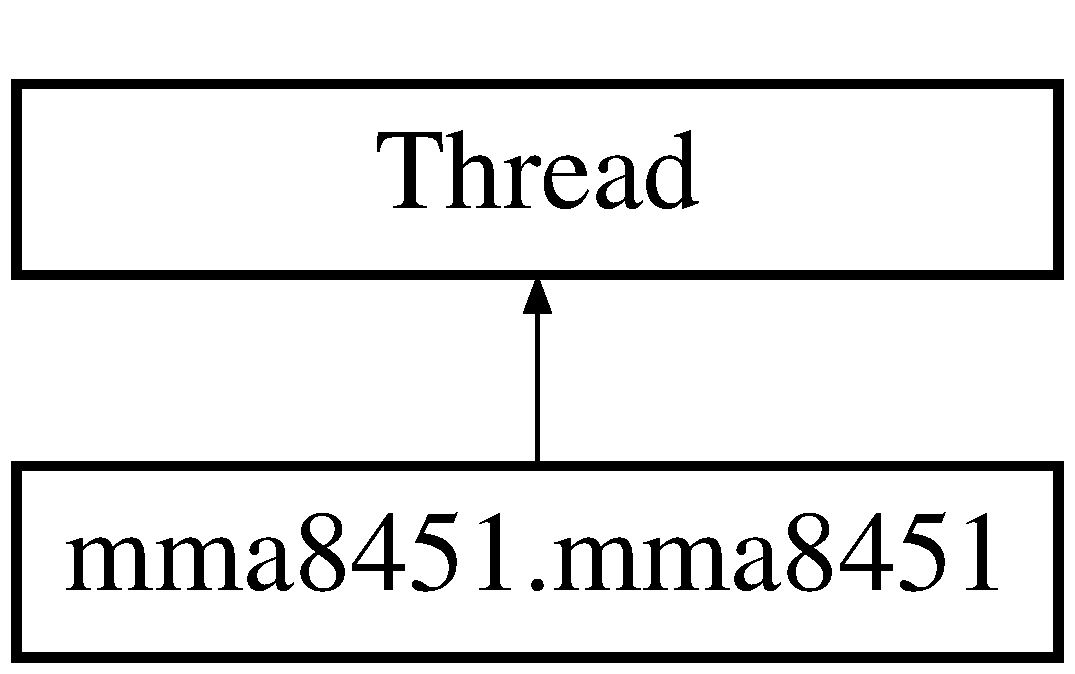
\includegraphics[height=2.000000cm]{classmma8451_1_1mma8451}
\end{center}
\end{figure}
\subsection*{Public Member Functions}
\begin{DoxyCompactItemize}
\item 
def \hyperlink{classmma8451_1_1mma8451_a778d5e81d0ed420045ef46e4e63ec2b8}{\+\_\+\+\_\+init\+\_\+\+\_\+} (self)
\item 
def \hyperlink{classmma8451_1_1mma8451_a41797c862f4ad2d8ef341056bb402c19}{read\+\_\+byte\+\_\+data} (self, register)
\item 
def \hyperlink{classmma8451_1_1mma8451_a8623dc076a6426e3946fb5c2482ba61a}{write\+\_\+byte\+\_\+data} (self, register, value)
\item 
def \hyperlink{classmma8451_1_1mma8451_a9a0d3d3fa5986b5d3ba43017c1d0e4d6}{check\+\_\+id} (self)
\item 
def \hyperlink{classmma8451_1_1mma8451_ae73bfb2314ef0a6175a73eb55c6a8584}{read\+\_\+raw\+\_\+xyz} (self)
\item 
def \hyperlink{classmma8451_1_1mma8451_af180360e06b1ad92a828f9b827723f7f}{read\+\_\+xyz} (self)
\item 
def \hyperlink{classmma8451_1_1mma8451_a540961793df44f27a640a1fbf90ed01b}{get\+\_\+int\+\_\+value} (self, val\+\_\+m, val\+\_\+l)
\item 
def \hyperlink{classmma8451_1_1mma8451_a2f5dadef2b037275ea03377643894fea}{set\+\_\+high\+\_\+pass\+\_\+filter} (self)
\item 
def \hyperlink{classmma8451_1_1mma8451_af83d50cf982bf4ecf898a8175fe9816a}{set\+\_\+range} (self, value)
\item 
def \hyperlink{classmma8451_1_1mma8451_a8d0a764cd5e7e33051f254f27eb2098f}{get\+\_\+data\+\_\+rate\+\_\+in\+\_\+hz} (self)
\item 
def \hyperlink{classmma8451_1_1mma8451_a7bfede66dd75d9d422775860818994db}{set\+\_\+data\+\_\+rate} (self, rate)
\item 
def \hyperlink{classmma8451_1_1mma8451_add58736fe80c5107ff4db30cff538222}{calibrate} (self)
\item 
def \hyperlink{classmma8451_1_1mma8451_a4eee718e56ce61a0b4284edde9f8de11}{run} (self)
\item 
def \hyperlink{classmma8451_1_1mma8451_a90b565e9288ddd6cd5a524d4d79837a7}{stop} (self)
\end{DoxyCompactItemize}
\subsection*{Public Attributes}
\begin{DoxyCompactItemize}
\item 
\hyperlink{classmma8451_1_1mma8451_a1cc6473d0eefeba3b11461b16a2d64f8}{measurement\+\_\+delay}
\item 
\hyperlink{classmma8451_1_1mma8451_a9fea18df9898f5f4df865a3668c29fbc}{bus}
\item 
\hyperlink{classmma8451_1_1mma8451_a5d0f9139629bb4316b3109e521368876}{step}
\item 
\hyperlink{classmma8451_1_1mma8451_a5051bf544957722f005045e8a16eb2e8}{sensor\+\_\+range}
\item 
\hyperlink{classmma8451_1_1mma8451_a1f58026a28067d044c257616c13ac318}{acceleration}
\item 
\hyperlink{classmma8451_1_1mma8451_abc10252bbf5c1468795d349f3ffcbcb0}{running}
\end{DoxyCompactItemize}
\subsection*{Static Public Attributes}
\begin{DoxyCompactItemize}
\item 
int \hyperlink{classmma8451_1_1mma8451_aa9153d7880ea51bce9a1a5d98a7da4cb}{D\+E\+V\+I\+C\+E\+\_\+\+A\+D\+DR} = 29
\item 
int \hyperlink{classmma8451_1_1mma8451_aee12eb3fb8955987eaeff1988f71183e}{D\+E\+V\+I\+C\+E\+\_\+\+ID} = 26
\item 
int \hyperlink{classmma8451_1_1mma8451_aead05ff6f6b975e0123dd9e018088766}{R\+E\+G\+\_\+\+S\+T\+A\+T\+US} = 0
\item 
int \hyperlink{classmma8451_1_1mma8451_a37a55007ad41f147b3e2ca3f7ccf9d92}{R\+E\+G\+\_\+\+O\+U\+T\+\_\+\+X\+\_\+\+M\+SB} = 1
\item 
int \hyperlink{classmma8451_1_1mma8451_aa6a391d4b295954e7b9975db171ad61c}{R\+E\+G\+\_\+\+O\+U\+T\+\_\+\+X\+\_\+\+L\+SB} = 2
\item 
int \hyperlink{classmma8451_1_1mma8451_ac8e77bf0b3b32e35adf38fc6f6300563}{R\+E\+G\+\_\+\+O\+U\+T\+\_\+\+Y\+\_\+\+M\+SB} = 3
\item 
int \hyperlink{classmma8451_1_1mma8451_ae468342bc61776475df5b62aff2c14ff}{R\+E\+G\+\_\+\+O\+U\+T\+\_\+\+Y\+\_\+\+L\+SB} = 4
\item 
int \hyperlink{classmma8451_1_1mma8451_ad692850016d4970724a6022a12b575c9}{R\+E\+G\+\_\+\+O\+U\+T\+\_\+\+Z\+\_\+\+M\+SB} = 5
\item 
int \hyperlink{classmma8451_1_1mma8451_ae5d8b2d00255d21c27ef92edc7c83b0f}{R\+E\+G\+\_\+\+O\+U\+T\+\_\+\+Z\+\_\+\+L\+SB} = 6
\item 
int \hyperlink{classmma8451_1_1mma8451_ac3b80c73531b9062452af93e67a44d93}{R\+E\+G\+\_\+\+S\+Y\+S\+M\+OD} = 11
\item 
int \hyperlink{classmma8451_1_1mma8451_a20a4e0571a8f9180c557e58d597aa01a}{R\+E\+G\+\_\+\+W\+H\+O\+A\+MI} = 13
\item 
int \hyperlink{classmma8451_1_1mma8451_a894171a505e26b83c85d3e3b0aa71be3}{R\+E\+G\+\_\+\+X\+Y\+Z\+\_\+\+D\+A\+T\+A\+\_\+\+C\+FG} = 14
\item 
int \hyperlink{classmma8451_1_1mma8451_a2e6ef1815928746311767a4d730428e3}{R\+E\+G\+\_\+\+X\+Y\+Z\+\_\+\+H\+PF} = 16
\item 
int \hyperlink{classmma8451_1_1mma8451_a597f8e72f78a6e3661e1247aa30f4a80}{R\+E\+G\+\_\+\+P\+L\+\_\+\+S\+T\+A\+T\+US} = 16
\item 
int \hyperlink{classmma8451_1_1mma8451_a7286e9ba7589d3c8931bb1273e14878c}{R\+E\+G\+\_\+\+P\+L\+\_\+\+C\+FG} = 17
\item 
int \hyperlink{classmma8451_1_1mma8451_a8326d71ec08fc3ab46e590e01c6c5e5e}{R\+E\+G1\+\_\+\+C\+T\+RL} = 42
\item 
int \hyperlink{classmma8451_1_1mma8451_a397c779fcf31f69d60acf0d9fd091bf3}{R\+E\+G2\+\_\+\+C\+T\+RL} = 43
\item 
int \hyperlink{classmma8451_1_1mma8451_a1e75cdb075f50da55a6001ca9621a459}{R\+E\+G4\+\_\+\+C\+T\+RL} = 45
\item 
int \hyperlink{classmma8451_1_1mma8451_a3a81ee7140f76b7b7febec54b22e64fe}{R\+E\+G5\+\_\+\+C\+T\+RL} = 46
\item 
int \hyperlink{classmma8451_1_1mma8451_afea71fa86d33a60e8346d4f447300a3c}{O\+F\+F\+\_\+X} = 47
\item 
int \hyperlink{classmma8451_1_1mma8451_a201f94b1fcb57e2eb85c36ee04561f72}{O\+F\+F\+\_\+Y} = 48
\item 
int \hyperlink{classmma8451_1_1mma8451_a9711d7d17e5c1f215523e1f0a1990f5b}{O\+F\+F\+\_\+Z} = 49
\item 
int \hyperlink{classmma8451_1_1mma8451_ad69d609cbce3f98e6d0203fc038673a1}{R\+E\+G\+\_\+\+X\+Y\+Z\+\_\+\+R\+A\+N\+G\+E\+\_\+8\+\_\+G} = 2
\item 
int \hyperlink{classmma8451_1_1mma8451_ac6ee56e5a622f588dbd538e1041e6367}{R\+E\+G\+\_\+\+X\+Y\+Z\+\_\+\+R\+A\+N\+G\+E\+\_\+4\+\_\+G} = 1
\item 
int \hyperlink{classmma8451_1_1mma8451_ac62b64468320473a459283f2331152c7}{R\+E\+G\+\_\+\+X\+Y\+Z\+\_\+\+R\+A\+N\+G\+E\+\_\+2\+\_\+G} = 0
\item 
int \hyperlink{classmma8451_1_1mma8451_a4e32292f76b78b01d9a06d625c8d305d}{R\+E\+G1\+\_\+\+A\+C\+T\+I\+VE} = 1
\item 
int \hyperlink{classmma8451_1_1mma8451_aa0595af0820e9008553320d475304799}{R\+E\+G1\+\_\+\+S\+T\+A\+N\+D\+BY} = 16
\item 
int \hyperlink{classmma8451_1_1mma8451_af61e366c70cfe918b04a7b153c200b7d}{R\+E\+G1\+\_\+\+F\+A\+S\+T\+\_\+\+R\+E\+AD} = 2
\item 
int \hyperlink{classmma8451_1_1mma8451_aee66b35034ab4680549d4771bc529b7d}{R\+E\+G1\+\_\+\+L\+O\+W\+\_\+\+N\+O\+I\+SE} = 4
\item 
int \hyperlink{classmma8451_1_1mma8451_a8398c8709186519753c349a78f4e3d23}{R\+E\+G1\+\_\+\+O\+DR} = 56
\item 
int \hyperlink{classmma8451_1_1mma8451_a82229a54ed10122cfebecaef1669084a}{R\+E\+G1\+\_\+\+O\+D\+R\+\_\+800\+\_\+\+HZ} = 0
\item 
int \hyperlink{classmma8451_1_1mma8451_a9246c231491e255487fdf52265603509}{R\+E\+G1\+\_\+\+O\+D\+R\+\_\+400\+\_\+\+HZ} = 8
\item 
int \hyperlink{classmma8451_1_1mma8451_a7a8c792a6f997b3e8f0782e37fc653c1}{R\+E\+G1\+\_\+\+O\+D\+R\+\_\+200\+\_\+\+HZ} = 16
\item 
int \hyperlink{classmma8451_1_1mma8451_aaaba8e0af3f800a17f99097584a7f2c2}{R\+E\+G1\+\_\+\+O\+D\+R\+\_\+100\+\_\+\+HZ} = 24
\item 
int \hyperlink{classmma8451_1_1mma8451_a1035e107cbfb9f8ea0bd8d9791aa392c}{R\+E\+G1\+\_\+\+O\+D\+R\+\_\+50\+\_\+\+HZ} = 32
\item 
int \hyperlink{classmma8451_1_1mma8451_a835a4efa1d33cde3e8091b8113b5dfd7}{R\+E\+G1\+\_\+\+O\+D\+R\+\_\+12\+\_\+5\+\_\+\+HZ} = 40
\item 
int \hyperlink{classmma8451_1_1mma8451_aa8417288dade1ee35f08210f2a86ce05}{R\+E\+G1\+\_\+\+O\+D\+R\+\_\+6\+\_\+25\+HZ} = 48
\item 
int \hyperlink{classmma8451_1_1mma8451_afa514ecabd97f94500f26256050f0d83}{R\+E\+G1\+\_\+\+O\+D\+R\+\_\+1\+\_\+56\+\_\+\+HZ} = 56
\item 
tuple \hyperlink{classmma8451_1_1mma8451_a189950c7292be13a56ef7822d0b37c3d}{R\+E\+G1\+\_\+\+O\+D\+R\+\_\+\+R\+A\+N\+GE}
\item 
int \hyperlink{classmma8451_1_1mma8451_a1ae300f552d1c1cef53720d5d5e32b22}{R\+E\+G2\+\_\+\+A\+U\+T\+O\+S\+L\+E\+EP} = 4
\item 
int \hyperlink{classmma8451_1_1mma8451_a472107dd3eb3308a4be8bdd5487c90d3}{R\+E\+G2\+\_\+\+R\+E\+S\+ET} = 64
\item 
int \hyperlink{classmma8451_1_1mma8451_ab4ba6823cb715bc63a83a109bb487900}{R\+E\+G2\+\_\+\+S\+E\+L\+F\+\_\+\+T\+E\+XT} = 128
\item 
int \hyperlink{classmma8451_1_1mma8451_a8860aa66ffd232be4ee16c7b6fc2075a}{R\+E\+G2\+\_\+\+A\+C\+T\+I\+V\+E\+\_\+\+O\+S\+\_\+\+N\+O\+R\+M\+AL} = 0
\item 
int \hyperlink{classmma8451_1_1mma8451_ae414025000132230109ebb73e7aec3b6}{R\+E\+G2\+\_\+\+A\+C\+T\+I\+V\+E\+\_\+\+O\+S\+\_\+\+L\+N\+O\+I\+S\+E\+\_\+\+L\+P\+O\+W\+ER} = 1
\item 
int \hyperlink{classmma8451_1_1mma8451_aefe76f264ec1028d2dd2ad1ccf99c800}{R\+E\+G2\+\_\+\+A\+C\+T\+I\+V\+E\+\_\+\+O\+S\+\_\+\+H\+I\+G\+H\+\_\+\+R\+E\+S\+O\+L\+U\+T\+I\+ON} = 2
\item 
int \hyperlink{classmma8451_1_1mma8451_aaf98f3185a208a6230116c75bbc744c4}{R\+E\+G2\+\_\+\+A\+C\+T\+I\+V\+E\+\_\+\+O\+S\+\_\+\+L\+O\+W\+\_\+\+P\+O\+W\+ER} = 3
\item 
int \hyperlink{classmma8451_1_1mma8451_a74aec4b06d390918a83a2a7989aa5db2}{R\+E\+G2\+\_\+\+S\+L\+E\+E\+P\+\_\+\+O\+S\+\_\+\+N\+O\+R\+M\+AL} = 0
\item 
int \hyperlink{classmma8451_1_1mma8451_a8bb6bdfb2c23b8648aeeefb358df6527}{R\+E\+G2\+\_\+\+S\+L\+E\+E\+P\+\_\+\+O\+S\+\_\+\+L\+N\+O\+I\+S\+E\+\_\+\+L\+P\+O\+W\+ER} = 8
\item 
int \hyperlink{classmma8451_1_1mma8451_aedb7d70ce73e28d19c3d01e968fd4b3c}{R\+E\+G2\+\_\+\+S\+L\+E\+E\+P\+\_\+\+O\+S\+\_\+\+H\+I\+G\+H\+\_\+\+R\+E\+S\+O\+L\+U\+T\+I\+ON} = 16
\item 
int \hyperlink{classmma8451_1_1mma8451_a9ff0d64dbc477357f9e60f5268dc8af6}{R\+E\+G2\+\_\+\+S\+L\+E\+E\+P\+\_\+\+O\+S\+\_\+\+L\+O\+W\+\_\+\+P\+O\+W\+ER} = 24
\end{DoxyCompactItemize}


\subsection{Constructor \& Destructor Documentation}
\mbox{\Hypertarget{classmma8451_1_1mma8451_a778d5e81d0ed420045ef46e4e63ec2b8}\label{classmma8451_1_1mma8451_a778d5e81d0ed420045ef46e4e63ec2b8}} 
\index{mma8451\+::mma8451@{mma8451\+::mma8451}!\+\_\+\+\_\+init\+\_\+\+\_\+@{\+\_\+\+\_\+init\+\_\+\+\_\+}}
\index{\+\_\+\+\_\+init\+\_\+\+\_\+@{\+\_\+\+\_\+init\+\_\+\+\_\+}!mma8451\+::mma8451@{mma8451\+::mma8451}}
\subsubsection{\texorpdfstring{\+\_\+\+\_\+init\+\_\+\+\_\+()}{\_\_init\_\_()}}
{\footnotesize\ttfamily def mma8451.\+mma8451.\+\_\+\+\_\+init\+\_\+\+\_\+ (\begin{DoxyParamCaption}\item[{}]{self }\end{DoxyParamCaption})}



\subsection{Member Function Documentation}
\mbox{\Hypertarget{classmma8451_1_1mma8451_add58736fe80c5107ff4db30cff538222}\label{classmma8451_1_1mma8451_add58736fe80c5107ff4db30cff538222}} 
\index{mma8451\+::mma8451@{mma8451\+::mma8451}!calibrate@{calibrate}}
\index{calibrate@{calibrate}!mma8451\+::mma8451@{mma8451\+::mma8451}}
\subsubsection{\texorpdfstring{calibrate()}{calibrate()}}
{\footnotesize\ttfamily def mma8451.\+mma8451.\+calibrate (\begin{DoxyParamCaption}\item[{}]{self }\end{DoxyParamCaption})}

\mbox{\Hypertarget{classmma8451_1_1mma8451_a9a0d3d3fa5986b5d3ba43017c1d0e4d6}\label{classmma8451_1_1mma8451_a9a0d3d3fa5986b5d3ba43017c1d0e4d6}} 
\index{mma8451\+::mma8451@{mma8451\+::mma8451}!check\+\_\+id@{check\+\_\+id}}
\index{check\+\_\+id@{check\+\_\+id}!mma8451\+::mma8451@{mma8451\+::mma8451}}
\subsubsection{\texorpdfstring{check\+\_\+id()}{check\_id()}}
{\footnotesize\ttfamily def mma8451.\+mma8451.\+check\+\_\+id (\begin{DoxyParamCaption}\item[{}]{self }\end{DoxyParamCaption})}

\mbox{\Hypertarget{classmma8451_1_1mma8451_a8d0a764cd5e7e33051f254f27eb2098f}\label{classmma8451_1_1mma8451_a8d0a764cd5e7e33051f254f27eb2098f}} 
\index{mma8451\+::mma8451@{mma8451\+::mma8451}!get\+\_\+data\+\_\+rate\+\_\+in\+\_\+hz@{get\+\_\+data\+\_\+rate\+\_\+in\+\_\+hz}}
\index{get\+\_\+data\+\_\+rate\+\_\+in\+\_\+hz@{get\+\_\+data\+\_\+rate\+\_\+in\+\_\+hz}!mma8451\+::mma8451@{mma8451\+::mma8451}}
\subsubsection{\texorpdfstring{get\+\_\+data\+\_\+rate\+\_\+in\+\_\+hz()}{get\_data\_rate\_in\_hz()}}
{\footnotesize\ttfamily def mma8451.\+mma8451.\+get\+\_\+data\+\_\+rate\+\_\+in\+\_\+hz (\begin{DoxyParamCaption}\item[{}]{self }\end{DoxyParamCaption})}

\mbox{\Hypertarget{classmma8451_1_1mma8451_a540961793df44f27a640a1fbf90ed01b}\label{classmma8451_1_1mma8451_a540961793df44f27a640a1fbf90ed01b}} 
\index{mma8451\+::mma8451@{mma8451\+::mma8451}!get\+\_\+int\+\_\+value@{get\+\_\+int\+\_\+value}}
\index{get\+\_\+int\+\_\+value@{get\+\_\+int\+\_\+value}!mma8451\+::mma8451@{mma8451\+::mma8451}}
\subsubsection{\texorpdfstring{get\+\_\+int\+\_\+value()}{get\_int\_value()}}
{\footnotesize\ttfamily def mma8451.\+mma8451.\+get\+\_\+int\+\_\+value (\begin{DoxyParamCaption}\item[{}]{self,  }\item[{}]{val\+\_\+m,  }\item[{}]{val\+\_\+l }\end{DoxyParamCaption})}

\mbox{\Hypertarget{classmma8451_1_1mma8451_a41797c862f4ad2d8ef341056bb402c19}\label{classmma8451_1_1mma8451_a41797c862f4ad2d8ef341056bb402c19}} 
\index{mma8451\+::mma8451@{mma8451\+::mma8451}!read\+\_\+byte\+\_\+data@{read\+\_\+byte\+\_\+data}}
\index{read\+\_\+byte\+\_\+data@{read\+\_\+byte\+\_\+data}!mma8451\+::mma8451@{mma8451\+::mma8451}}
\subsubsection{\texorpdfstring{read\+\_\+byte\+\_\+data()}{read\_byte\_data()}}
{\footnotesize\ttfamily def mma8451.\+mma8451.\+read\+\_\+byte\+\_\+data (\begin{DoxyParamCaption}\item[{}]{self,  }\item[{}]{register }\end{DoxyParamCaption})}

\mbox{\Hypertarget{classmma8451_1_1mma8451_ae73bfb2314ef0a6175a73eb55c6a8584}\label{classmma8451_1_1mma8451_ae73bfb2314ef0a6175a73eb55c6a8584}} 
\index{mma8451\+::mma8451@{mma8451\+::mma8451}!read\+\_\+raw\+\_\+xyz@{read\+\_\+raw\+\_\+xyz}}
\index{read\+\_\+raw\+\_\+xyz@{read\+\_\+raw\+\_\+xyz}!mma8451\+::mma8451@{mma8451\+::mma8451}}
\subsubsection{\texorpdfstring{read\+\_\+raw\+\_\+xyz()}{read\_raw\_xyz()}}
{\footnotesize\ttfamily def mma8451.\+mma8451.\+read\+\_\+raw\+\_\+xyz (\begin{DoxyParamCaption}\item[{}]{self }\end{DoxyParamCaption})}

\mbox{\Hypertarget{classmma8451_1_1mma8451_af180360e06b1ad92a828f9b827723f7f}\label{classmma8451_1_1mma8451_af180360e06b1ad92a828f9b827723f7f}} 
\index{mma8451\+::mma8451@{mma8451\+::mma8451}!read\+\_\+xyz@{read\+\_\+xyz}}
\index{read\+\_\+xyz@{read\+\_\+xyz}!mma8451\+::mma8451@{mma8451\+::mma8451}}
\subsubsection{\texorpdfstring{read\+\_\+xyz()}{read\_xyz()}}
{\footnotesize\ttfamily def mma8451.\+mma8451.\+read\+\_\+xyz (\begin{DoxyParamCaption}\item[{}]{self }\end{DoxyParamCaption})}

\mbox{\Hypertarget{classmma8451_1_1mma8451_a4eee718e56ce61a0b4284edde9f8de11}\label{classmma8451_1_1mma8451_a4eee718e56ce61a0b4284edde9f8de11}} 
\index{mma8451\+::mma8451@{mma8451\+::mma8451}!run@{run}}
\index{run@{run}!mma8451\+::mma8451@{mma8451\+::mma8451}}
\subsubsection{\texorpdfstring{run()}{run()}}
{\footnotesize\ttfamily def mma8451.\+mma8451.\+run (\begin{DoxyParamCaption}\item[{}]{self }\end{DoxyParamCaption})}

\mbox{\Hypertarget{classmma8451_1_1mma8451_a7bfede66dd75d9d422775860818994db}\label{classmma8451_1_1mma8451_a7bfede66dd75d9d422775860818994db}} 
\index{mma8451\+::mma8451@{mma8451\+::mma8451}!set\+\_\+data\+\_\+rate@{set\+\_\+data\+\_\+rate}}
\index{set\+\_\+data\+\_\+rate@{set\+\_\+data\+\_\+rate}!mma8451\+::mma8451@{mma8451\+::mma8451}}
\subsubsection{\texorpdfstring{set\+\_\+data\+\_\+rate()}{set\_data\_rate()}}
{\footnotesize\ttfamily def mma8451.\+mma8451.\+set\+\_\+data\+\_\+rate (\begin{DoxyParamCaption}\item[{}]{self,  }\item[{}]{rate }\end{DoxyParamCaption})}

\mbox{\Hypertarget{classmma8451_1_1mma8451_a2f5dadef2b037275ea03377643894fea}\label{classmma8451_1_1mma8451_a2f5dadef2b037275ea03377643894fea}} 
\index{mma8451\+::mma8451@{mma8451\+::mma8451}!set\+\_\+high\+\_\+pass\+\_\+filter@{set\+\_\+high\+\_\+pass\+\_\+filter}}
\index{set\+\_\+high\+\_\+pass\+\_\+filter@{set\+\_\+high\+\_\+pass\+\_\+filter}!mma8451\+::mma8451@{mma8451\+::mma8451}}
\subsubsection{\texorpdfstring{set\+\_\+high\+\_\+pass\+\_\+filter()}{set\_high\_pass\_filter()}}
{\footnotesize\ttfamily def mma8451.\+mma8451.\+set\+\_\+high\+\_\+pass\+\_\+filter (\begin{DoxyParamCaption}\item[{}]{self }\end{DoxyParamCaption})}

\mbox{\Hypertarget{classmma8451_1_1mma8451_af83d50cf982bf4ecf898a8175fe9816a}\label{classmma8451_1_1mma8451_af83d50cf982bf4ecf898a8175fe9816a}} 
\index{mma8451\+::mma8451@{mma8451\+::mma8451}!set\+\_\+range@{set\+\_\+range}}
\index{set\+\_\+range@{set\+\_\+range}!mma8451\+::mma8451@{mma8451\+::mma8451}}
\subsubsection{\texorpdfstring{set\+\_\+range()}{set\_range()}}
{\footnotesize\ttfamily def mma8451.\+mma8451.\+set\+\_\+range (\begin{DoxyParamCaption}\item[{}]{self,  }\item[{}]{value }\end{DoxyParamCaption})}

\mbox{\Hypertarget{classmma8451_1_1mma8451_a90b565e9288ddd6cd5a524d4d79837a7}\label{classmma8451_1_1mma8451_a90b565e9288ddd6cd5a524d4d79837a7}} 
\index{mma8451\+::mma8451@{mma8451\+::mma8451}!stop@{stop}}
\index{stop@{stop}!mma8451\+::mma8451@{mma8451\+::mma8451}}
\subsubsection{\texorpdfstring{stop()}{stop()}}
{\footnotesize\ttfamily def mma8451.\+mma8451.\+stop (\begin{DoxyParamCaption}\item[{}]{self }\end{DoxyParamCaption})}

\mbox{\Hypertarget{classmma8451_1_1mma8451_a8623dc076a6426e3946fb5c2482ba61a}\label{classmma8451_1_1mma8451_a8623dc076a6426e3946fb5c2482ba61a}} 
\index{mma8451\+::mma8451@{mma8451\+::mma8451}!write\+\_\+byte\+\_\+data@{write\+\_\+byte\+\_\+data}}
\index{write\+\_\+byte\+\_\+data@{write\+\_\+byte\+\_\+data}!mma8451\+::mma8451@{mma8451\+::mma8451}}
\subsubsection{\texorpdfstring{write\+\_\+byte\+\_\+data()}{write\_byte\_data()}}
{\footnotesize\ttfamily def mma8451.\+mma8451.\+write\+\_\+byte\+\_\+data (\begin{DoxyParamCaption}\item[{}]{self,  }\item[{}]{register,  }\item[{}]{value }\end{DoxyParamCaption})}



\subsection{Member Data Documentation}
\mbox{\Hypertarget{classmma8451_1_1mma8451_a1f58026a28067d044c257616c13ac318}\label{classmma8451_1_1mma8451_a1f58026a28067d044c257616c13ac318}} 
\index{mma8451\+::mma8451@{mma8451\+::mma8451}!acceleration@{acceleration}}
\index{acceleration@{acceleration}!mma8451\+::mma8451@{mma8451\+::mma8451}}
\subsubsection{\texorpdfstring{acceleration}{acceleration}}
{\footnotesize\ttfamily mma8451.\+mma8451.\+acceleration}

\mbox{\Hypertarget{classmma8451_1_1mma8451_a9fea18df9898f5f4df865a3668c29fbc}\label{classmma8451_1_1mma8451_a9fea18df9898f5f4df865a3668c29fbc}} 
\index{mma8451\+::mma8451@{mma8451\+::mma8451}!bus@{bus}}
\index{bus@{bus}!mma8451\+::mma8451@{mma8451\+::mma8451}}
\subsubsection{\texorpdfstring{bus}{bus}}
{\footnotesize\ttfamily mma8451.\+mma8451.\+bus}

\mbox{\Hypertarget{classmma8451_1_1mma8451_aa9153d7880ea51bce9a1a5d98a7da4cb}\label{classmma8451_1_1mma8451_aa9153d7880ea51bce9a1a5d98a7da4cb}} 
\index{mma8451\+::mma8451@{mma8451\+::mma8451}!D\+E\+V\+I\+C\+E\+\_\+\+A\+D\+DR@{D\+E\+V\+I\+C\+E\+\_\+\+A\+D\+DR}}
\index{D\+E\+V\+I\+C\+E\+\_\+\+A\+D\+DR@{D\+E\+V\+I\+C\+E\+\_\+\+A\+D\+DR}!mma8451\+::mma8451@{mma8451\+::mma8451}}
\subsubsection{\texorpdfstring{D\+E\+V\+I\+C\+E\+\_\+\+A\+D\+DR}{DEVICE\_ADDR}}
{\footnotesize\ttfamily int mma8451.\+mma8451.\+D\+E\+V\+I\+C\+E\+\_\+\+A\+D\+DR = 29\hspace{0.3cm}{\ttfamily [static]}}

\mbox{\Hypertarget{classmma8451_1_1mma8451_aee12eb3fb8955987eaeff1988f71183e}\label{classmma8451_1_1mma8451_aee12eb3fb8955987eaeff1988f71183e}} 
\index{mma8451\+::mma8451@{mma8451\+::mma8451}!D\+E\+V\+I\+C\+E\+\_\+\+ID@{D\+E\+V\+I\+C\+E\+\_\+\+ID}}
\index{D\+E\+V\+I\+C\+E\+\_\+\+ID@{D\+E\+V\+I\+C\+E\+\_\+\+ID}!mma8451\+::mma8451@{mma8451\+::mma8451}}
\subsubsection{\texorpdfstring{D\+E\+V\+I\+C\+E\+\_\+\+ID}{DEVICE\_ID}}
{\footnotesize\ttfamily int mma8451.\+mma8451.\+D\+E\+V\+I\+C\+E\+\_\+\+ID = 26\hspace{0.3cm}{\ttfamily [static]}}

\mbox{\Hypertarget{classmma8451_1_1mma8451_a1cc6473d0eefeba3b11461b16a2d64f8}\label{classmma8451_1_1mma8451_a1cc6473d0eefeba3b11461b16a2d64f8}} 
\index{mma8451\+::mma8451@{mma8451\+::mma8451}!measurement\+\_\+delay@{measurement\+\_\+delay}}
\index{measurement\+\_\+delay@{measurement\+\_\+delay}!mma8451\+::mma8451@{mma8451\+::mma8451}}
\subsubsection{\texorpdfstring{measurement\+\_\+delay}{measurement\_delay}}
{\footnotesize\ttfamily mma8451.\+mma8451.\+measurement\+\_\+delay}

\mbox{\Hypertarget{classmma8451_1_1mma8451_afea71fa86d33a60e8346d4f447300a3c}\label{classmma8451_1_1mma8451_afea71fa86d33a60e8346d4f447300a3c}} 
\index{mma8451\+::mma8451@{mma8451\+::mma8451}!O\+F\+F\+\_\+X@{O\+F\+F\+\_\+X}}
\index{O\+F\+F\+\_\+X@{O\+F\+F\+\_\+X}!mma8451\+::mma8451@{mma8451\+::mma8451}}
\subsubsection{\texorpdfstring{O\+F\+F\+\_\+X}{OFF\_X}}
{\footnotesize\ttfamily int mma8451.\+mma8451.\+O\+F\+F\+\_\+X = 47\hspace{0.3cm}{\ttfamily [static]}}

\mbox{\Hypertarget{classmma8451_1_1mma8451_a201f94b1fcb57e2eb85c36ee04561f72}\label{classmma8451_1_1mma8451_a201f94b1fcb57e2eb85c36ee04561f72}} 
\index{mma8451\+::mma8451@{mma8451\+::mma8451}!O\+F\+F\+\_\+Y@{O\+F\+F\+\_\+Y}}
\index{O\+F\+F\+\_\+Y@{O\+F\+F\+\_\+Y}!mma8451\+::mma8451@{mma8451\+::mma8451}}
\subsubsection{\texorpdfstring{O\+F\+F\+\_\+Y}{OFF\_Y}}
{\footnotesize\ttfamily int mma8451.\+mma8451.\+O\+F\+F\+\_\+Y = 48\hspace{0.3cm}{\ttfamily [static]}}

\mbox{\Hypertarget{classmma8451_1_1mma8451_a9711d7d17e5c1f215523e1f0a1990f5b}\label{classmma8451_1_1mma8451_a9711d7d17e5c1f215523e1f0a1990f5b}} 
\index{mma8451\+::mma8451@{mma8451\+::mma8451}!O\+F\+F\+\_\+Z@{O\+F\+F\+\_\+Z}}
\index{O\+F\+F\+\_\+Z@{O\+F\+F\+\_\+Z}!mma8451\+::mma8451@{mma8451\+::mma8451}}
\subsubsection{\texorpdfstring{O\+F\+F\+\_\+Z}{OFF\_Z}}
{\footnotesize\ttfamily int mma8451.\+mma8451.\+O\+F\+F\+\_\+Z = 49\hspace{0.3cm}{\ttfamily [static]}}

\mbox{\Hypertarget{classmma8451_1_1mma8451_a4e32292f76b78b01d9a06d625c8d305d}\label{classmma8451_1_1mma8451_a4e32292f76b78b01d9a06d625c8d305d}} 
\index{mma8451\+::mma8451@{mma8451\+::mma8451}!R\+E\+G1\+\_\+\+A\+C\+T\+I\+VE@{R\+E\+G1\+\_\+\+A\+C\+T\+I\+VE}}
\index{R\+E\+G1\+\_\+\+A\+C\+T\+I\+VE@{R\+E\+G1\+\_\+\+A\+C\+T\+I\+VE}!mma8451\+::mma8451@{mma8451\+::mma8451}}
\subsubsection{\texorpdfstring{R\+E\+G1\+\_\+\+A\+C\+T\+I\+VE}{REG1\_ACTIVE}}
{\footnotesize\ttfamily int mma8451.\+mma8451.\+R\+E\+G1\+\_\+\+A\+C\+T\+I\+VE = 1\hspace{0.3cm}{\ttfamily [static]}}

\mbox{\Hypertarget{classmma8451_1_1mma8451_a8326d71ec08fc3ab46e590e01c6c5e5e}\label{classmma8451_1_1mma8451_a8326d71ec08fc3ab46e590e01c6c5e5e}} 
\index{mma8451\+::mma8451@{mma8451\+::mma8451}!R\+E\+G1\+\_\+\+C\+T\+RL@{R\+E\+G1\+\_\+\+C\+T\+RL}}
\index{R\+E\+G1\+\_\+\+C\+T\+RL@{R\+E\+G1\+\_\+\+C\+T\+RL}!mma8451\+::mma8451@{mma8451\+::mma8451}}
\subsubsection{\texorpdfstring{R\+E\+G1\+\_\+\+C\+T\+RL}{REG1\_CTRL}}
{\footnotesize\ttfamily int mma8451.\+mma8451.\+R\+E\+G1\+\_\+\+C\+T\+RL = 42\hspace{0.3cm}{\ttfamily [static]}}

\mbox{\Hypertarget{classmma8451_1_1mma8451_af61e366c70cfe918b04a7b153c200b7d}\label{classmma8451_1_1mma8451_af61e366c70cfe918b04a7b153c200b7d}} 
\index{mma8451\+::mma8451@{mma8451\+::mma8451}!R\+E\+G1\+\_\+\+F\+A\+S\+T\+\_\+\+R\+E\+AD@{R\+E\+G1\+\_\+\+F\+A\+S\+T\+\_\+\+R\+E\+AD}}
\index{R\+E\+G1\+\_\+\+F\+A\+S\+T\+\_\+\+R\+E\+AD@{R\+E\+G1\+\_\+\+F\+A\+S\+T\+\_\+\+R\+E\+AD}!mma8451\+::mma8451@{mma8451\+::mma8451}}
\subsubsection{\texorpdfstring{R\+E\+G1\+\_\+\+F\+A\+S\+T\+\_\+\+R\+E\+AD}{REG1\_FAST\_READ}}
{\footnotesize\ttfamily int mma8451.\+mma8451.\+R\+E\+G1\+\_\+\+F\+A\+S\+T\+\_\+\+R\+E\+AD = 2\hspace{0.3cm}{\ttfamily [static]}}

\mbox{\Hypertarget{classmma8451_1_1mma8451_aee66b35034ab4680549d4771bc529b7d}\label{classmma8451_1_1mma8451_aee66b35034ab4680549d4771bc529b7d}} 
\index{mma8451\+::mma8451@{mma8451\+::mma8451}!R\+E\+G1\+\_\+\+L\+O\+W\+\_\+\+N\+O\+I\+SE@{R\+E\+G1\+\_\+\+L\+O\+W\+\_\+\+N\+O\+I\+SE}}
\index{R\+E\+G1\+\_\+\+L\+O\+W\+\_\+\+N\+O\+I\+SE@{R\+E\+G1\+\_\+\+L\+O\+W\+\_\+\+N\+O\+I\+SE}!mma8451\+::mma8451@{mma8451\+::mma8451}}
\subsubsection{\texorpdfstring{R\+E\+G1\+\_\+\+L\+O\+W\+\_\+\+N\+O\+I\+SE}{REG1\_LOW\_NOISE}}
{\footnotesize\ttfamily int mma8451.\+mma8451.\+R\+E\+G1\+\_\+\+L\+O\+W\+\_\+\+N\+O\+I\+SE = 4\hspace{0.3cm}{\ttfamily [static]}}

\mbox{\Hypertarget{classmma8451_1_1mma8451_a8398c8709186519753c349a78f4e3d23}\label{classmma8451_1_1mma8451_a8398c8709186519753c349a78f4e3d23}} 
\index{mma8451\+::mma8451@{mma8451\+::mma8451}!R\+E\+G1\+\_\+\+O\+DR@{R\+E\+G1\+\_\+\+O\+DR}}
\index{R\+E\+G1\+\_\+\+O\+DR@{R\+E\+G1\+\_\+\+O\+DR}!mma8451\+::mma8451@{mma8451\+::mma8451}}
\subsubsection{\texorpdfstring{R\+E\+G1\+\_\+\+O\+DR}{REG1\_ODR}}
{\footnotesize\ttfamily int mma8451.\+mma8451.\+R\+E\+G1\+\_\+\+O\+DR = 56\hspace{0.3cm}{\ttfamily [static]}}

\mbox{\Hypertarget{classmma8451_1_1mma8451_aaaba8e0af3f800a17f99097584a7f2c2}\label{classmma8451_1_1mma8451_aaaba8e0af3f800a17f99097584a7f2c2}} 
\index{mma8451\+::mma8451@{mma8451\+::mma8451}!R\+E\+G1\+\_\+\+O\+D\+R\+\_\+100\+\_\+\+HZ@{R\+E\+G1\+\_\+\+O\+D\+R\+\_\+100\+\_\+\+HZ}}
\index{R\+E\+G1\+\_\+\+O\+D\+R\+\_\+100\+\_\+\+HZ@{R\+E\+G1\+\_\+\+O\+D\+R\+\_\+100\+\_\+\+HZ}!mma8451\+::mma8451@{mma8451\+::mma8451}}
\subsubsection{\texorpdfstring{R\+E\+G1\+\_\+\+O\+D\+R\+\_\+100\+\_\+\+HZ}{REG1\_ODR\_100\_HZ}}
{\footnotesize\ttfamily int mma8451.\+mma8451.\+R\+E\+G1\+\_\+\+O\+D\+R\+\_\+100\+\_\+\+HZ = 24\hspace{0.3cm}{\ttfamily [static]}}

\mbox{\Hypertarget{classmma8451_1_1mma8451_a835a4efa1d33cde3e8091b8113b5dfd7}\label{classmma8451_1_1mma8451_a835a4efa1d33cde3e8091b8113b5dfd7}} 
\index{mma8451\+::mma8451@{mma8451\+::mma8451}!R\+E\+G1\+\_\+\+O\+D\+R\+\_\+12\+\_\+5\+\_\+\+HZ@{R\+E\+G1\+\_\+\+O\+D\+R\+\_\+12\+\_\+5\+\_\+\+HZ}}
\index{R\+E\+G1\+\_\+\+O\+D\+R\+\_\+12\+\_\+5\+\_\+\+HZ@{R\+E\+G1\+\_\+\+O\+D\+R\+\_\+12\+\_\+5\+\_\+\+HZ}!mma8451\+::mma8451@{mma8451\+::mma8451}}
\subsubsection{\texorpdfstring{R\+E\+G1\+\_\+\+O\+D\+R\+\_\+12\+\_\+5\+\_\+\+HZ}{REG1\_ODR\_12\_5\_HZ}}
{\footnotesize\ttfamily int mma8451.\+mma8451.\+R\+E\+G1\+\_\+\+O\+D\+R\+\_\+12\+\_\+5\+\_\+\+HZ = 40\hspace{0.3cm}{\ttfamily [static]}}

\mbox{\Hypertarget{classmma8451_1_1mma8451_afa514ecabd97f94500f26256050f0d83}\label{classmma8451_1_1mma8451_afa514ecabd97f94500f26256050f0d83}} 
\index{mma8451\+::mma8451@{mma8451\+::mma8451}!R\+E\+G1\+\_\+\+O\+D\+R\+\_\+1\+\_\+56\+\_\+\+HZ@{R\+E\+G1\+\_\+\+O\+D\+R\+\_\+1\+\_\+56\+\_\+\+HZ}}
\index{R\+E\+G1\+\_\+\+O\+D\+R\+\_\+1\+\_\+56\+\_\+\+HZ@{R\+E\+G1\+\_\+\+O\+D\+R\+\_\+1\+\_\+56\+\_\+\+HZ}!mma8451\+::mma8451@{mma8451\+::mma8451}}
\subsubsection{\texorpdfstring{R\+E\+G1\+\_\+\+O\+D\+R\+\_\+1\+\_\+56\+\_\+\+HZ}{REG1\_ODR\_1\_56\_HZ}}
{\footnotesize\ttfamily int mma8451.\+mma8451.\+R\+E\+G1\+\_\+\+O\+D\+R\+\_\+1\+\_\+56\+\_\+\+HZ = 56\hspace{0.3cm}{\ttfamily [static]}}

\mbox{\Hypertarget{classmma8451_1_1mma8451_a7a8c792a6f997b3e8f0782e37fc653c1}\label{classmma8451_1_1mma8451_a7a8c792a6f997b3e8f0782e37fc653c1}} 
\index{mma8451\+::mma8451@{mma8451\+::mma8451}!R\+E\+G1\+\_\+\+O\+D\+R\+\_\+200\+\_\+\+HZ@{R\+E\+G1\+\_\+\+O\+D\+R\+\_\+200\+\_\+\+HZ}}
\index{R\+E\+G1\+\_\+\+O\+D\+R\+\_\+200\+\_\+\+HZ@{R\+E\+G1\+\_\+\+O\+D\+R\+\_\+200\+\_\+\+HZ}!mma8451\+::mma8451@{mma8451\+::mma8451}}
\subsubsection{\texorpdfstring{R\+E\+G1\+\_\+\+O\+D\+R\+\_\+200\+\_\+\+HZ}{REG1\_ODR\_200\_HZ}}
{\footnotesize\ttfamily int mma8451.\+mma8451.\+R\+E\+G1\+\_\+\+O\+D\+R\+\_\+200\+\_\+\+HZ = 16\hspace{0.3cm}{\ttfamily [static]}}

\mbox{\Hypertarget{classmma8451_1_1mma8451_a9246c231491e255487fdf52265603509}\label{classmma8451_1_1mma8451_a9246c231491e255487fdf52265603509}} 
\index{mma8451\+::mma8451@{mma8451\+::mma8451}!R\+E\+G1\+\_\+\+O\+D\+R\+\_\+400\+\_\+\+HZ@{R\+E\+G1\+\_\+\+O\+D\+R\+\_\+400\+\_\+\+HZ}}
\index{R\+E\+G1\+\_\+\+O\+D\+R\+\_\+400\+\_\+\+HZ@{R\+E\+G1\+\_\+\+O\+D\+R\+\_\+400\+\_\+\+HZ}!mma8451\+::mma8451@{mma8451\+::mma8451}}
\subsubsection{\texorpdfstring{R\+E\+G1\+\_\+\+O\+D\+R\+\_\+400\+\_\+\+HZ}{REG1\_ODR\_400\_HZ}}
{\footnotesize\ttfamily int mma8451.\+mma8451.\+R\+E\+G1\+\_\+\+O\+D\+R\+\_\+400\+\_\+\+HZ = 8\hspace{0.3cm}{\ttfamily [static]}}

\mbox{\Hypertarget{classmma8451_1_1mma8451_a1035e107cbfb9f8ea0bd8d9791aa392c}\label{classmma8451_1_1mma8451_a1035e107cbfb9f8ea0bd8d9791aa392c}} 
\index{mma8451\+::mma8451@{mma8451\+::mma8451}!R\+E\+G1\+\_\+\+O\+D\+R\+\_\+50\+\_\+\+HZ@{R\+E\+G1\+\_\+\+O\+D\+R\+\_\+50\+\_\+\+HZ}}
\index{R\+E\+G1\+\_\+\+O\+D\+R\+\_\+50\+\_\+\+HZ@{R\+E\+G1\+\_\+\+O\+D\+R\+\_\+50\+\_\+\+HZ}!mma8451\+::mma8451@{mma8451\+::mma8451}}
\subsubsection{\texorpdfstring{R\+E\+G1\+\_\+\+O\+D\+R\+\_\+50\+\_\+\+HZ}{REG1\_ODR\_50\_HZ}}
{\footnotesize\ttfamily int mma8451.\+mma8451.\+R\+E\+G1\+\_\+\+O\+D\+R\+\_\+50\+\_\+\+HZ = 32\hspace{0.3cm}{\ttfamily [static]}}

\mbox{\Hypertarget{classmma8451_1_1mma8451_aa8417288dade1ee35f08210f2a86ce05}\label{classmma8451_1_1mma8451_aa8417288dade1ee35f08210f2a86ce05}} 
\index{mma8451\+::mma8451@{mma8451\+::mma8451}!R\+E\+G1\+\_\+\+O\+D\+R\+\_\+6\+\_\+25\+HZ@{R\+E\+G1\+\_\+\+O\+D\+R\+\_\+6\+\_\+25\+HZ}}
\index{R\+E\+G1\+\_\+\+O\+D\+R\+\_\+6\+\_\+25\+HZ@{R\+E\+G1\+\_\+\+O\+D\+R\+\_\+6\+\_\+25\+HZ}!mma8451\+::mma8451@{mma8451\+::mma8451}}
\subsubsection{\texorpdfstring{R\+E\+G1\+\_\+\+O\+D\+R\+\_\+6\+\_\+25\+HZ}{REG1\_ODR\_6\_25HZ}}
{\footnotesize\ttfamily int mma8451.\+mma8451.\+R\+E\+G1\+\_\+\+O\+D\+R\+\_\+6\+\_\+25\+HZ = 48\hspace{0.3cm}{\ttfamily [static]}}

\mbox{\Hypertarget{classmma8451_1_1mma8451_a82229a54ed10122cfebecaef1669084a}\label{classmma8451_1_1mma8451_a82229a54ed10122cfebecaef1669084a}} 
\index{mma8451\+::mma8451@{mma8451\+::mma8451}!R\+E\+G1\+\_\+\+O\+D\+R\+\_\+800\+\_\+\+HZ@{R\+E\+G1\+\_\+\+O\+D\+R\+\_\+800\+\_\+\+HZ}}
\index{R\+E\+G1\+\_\+\+O\+D\+R\+\_\+800\+\_\+\+HZ@{R\+E\+G1\+\_\+\+O\+D\+R\+\_\+800\+\_\+\+HZ}!mma8451\+::mma8451@{mma8451\+::mma8451}}
\subsubsection{\texorpdfstring{R\+E\+G1\+\_\+\+O\+D\+R\+\_\+800\+\_\+\+HZ}{REG1\_ODR\_800\_HZ}}
{\footnotesize\ttfamily int mma8451.\+mma8451.\+R\+E\+G1\+\_\+\+O\+D\+R\+\_\+800\+\_\+\+HZ = 0\hspace{0.3cm}{\ttfamily [static]}}

\mbox{\Hypertarget{classmma8451_1_1mma8451_a189950c7292be13a56ef7822d0b37c3d}\label{classmma8451_1_1mma8451_a189950c7292be13a56ef7822d0b37c3d}} 
\index{mma8451\+::mma8451@{mma8451\+::mma8451}!R\+E\+G1\+\_\+\+O\+D\+R\+\_\+\+R\+A\+N\+GE@{R\+E\+G1\+\_\+\+O\+D\+R\+\_\+\+R\+A\+N\+GE}}
\index{R\+E\+G1\+\_\+\+O\+D\+R\+\_\+\+R\+A\+N\+GE@{R\+E\+G1\+\_\+\+O\+D\+R\+\_\+\+R\+A\+N\+GE}!mma8451\+::mma8451@{mma8451\+::mma8451}}
\subsubsection{\texorpdfstring{R\+E\+G1\+\_\+\+O\+D\+R\+\_\+\+R\+A\+N\+GE}{REG1\_ODR\_RANGE}}
{\footnotesize\ttfamily tuple mma8451.\+mma8451.\+R\+E\+G1\+\_\+\+O\+D\+R\+\_\+\+R\+A\+N\+GE\hspace{0.3cm}{\ttfamily [static]}}

{\bfseries Initial value\+:}
\begin{DoxyCode}
=  (REG1\_ODR\_800\_HZ,
                      REG1\_ODR\_400\_HZ,
                      REG1\_ODR\_200\_HZ,
                      REG1\_ODR\_100\_HZ,
                      REG1\_ODR\_50\_HZ,
                      REG1\_ODR\_12\_5\_HZ,
                      REG1\_ODR\_6\_25HZ,
                      REG1\_ODR\_1\_56\_HZ)
\end{DoxyCode}
\mbox{\Hypertarget{classmma8451_1_1mma8451_aa0595af0820e9008553320d475304799}\label{classmma8451_1_1mma8451_aa0595af0820e9008553320d475304799}} 
\index{mma8451\+::mma8451@{mma8451\+::mma8451}!R\+E\+G1\+\_\+\+S\+T\+A\+N\+D\+BY@{R\+E\+G1\+\_\+\+S\+T\+A\+N\+D\+BY}}
\index{R\+E\+G1\+\_\+\+S\+T\+A\+N\+D\+BY@{R\+E\+G1\+\_\+\+S\+T\+A\+N\+D\+BY}!mma8451\+::mma8451@{mma8451\+::mma8451}}
\subsubsection{\texorpdfstring{R\+E\+G1\+\_\+\+S\+T\+A\+N\+D\+BY}{REG1\_STANDBY}}
{\footnotesize\ttfamily int mma8451.\+mma8451.\+R\+E\+G1\+\_\+\+S\+T\+A\+N\+D\+BY = 16\hspace{0.3cm}{\ttfamily [static]}}

\mbox{\Hypertarget{classmma8451_1_1mma8451_aefe76f264ec1028d2dd2ad1ccf99c800}\label{classmma8451_1_1mma8451_aefe76f264ec1028d2dd2ad1ccf99c800}} 
\index{mma8451\+::mma8451@{mma8451\+::mma8451}!R\+E\+G2\+\_\+\+A\+C\+T\+I\+V\+E\+\_\+\+O\+S\+\_\+\+H\+I\+G\+H\+\_\+\+R\+E\+S\+O\+L\+U\+T\+I\+ON@{R\+E\+G2\+\_\+\+A\+C\+T\+I\+V\+E\+\_\+\+O\+S\+\_\+\+H\+I\+G\+H\+\_\+\+R\+E\+S\+O\+L\+U\+T\+I\+ON}}
\index{R\+E\+G2\+\_\+\+A\+C\+T\+I\+V\+E\+\_\+\+O\+S\+\_\+\+H\+I\+G\+H\+\_\+\+R\+E\+S\+O\+L\+U\+T\+I\+ON@{R\+E\+G2\+\_\+\+A\+C\+T\+I\+V\+E\+\_\+\+O\+S\+\_\+\+H\+I\+G\+H\+\_\+\+R\+E\+S\+O\+L\+U\+T\+I\+ON}!mma8451\+::mma8451@{mma8451\+::mma8451}}
\subsubsection{\texorpdfstring{R\+E\+G2\+\_\+\+A\+C\+T\+I\+V\+E\+\_\+\+O\+S\+\_\+\+H\+I\+G\+H\+\_\+\+R\+E\+S\+O\+L\+U\+T\+I\+ON}{REG2\_ACTIVE\_OS\_HIGH\_RESOLUTION}}
{\footnotesize\ttfamily int mma8451.\+mma8451.\+R\+E\+G2\+\_\+\+A\+C\+T\+I\+V\+E\+\_\+\+O\+S\+\_\+\+H\+I\+G\+H\+\_\+\+R\+E\+S\+O\+L\+U\+T\+I\+ON = 2\hspace{0.3cm}{\ttfamily [static]}}

\mbox{\Hypertarget{classmma8451_1_1mma8451_ae414025000132230109ebb73e7aec3b6}\label{classmma8451_1_1mma8451_ae414025000132230109ebb73e7aec3b6}} 
\index{mma8451\+::mma8451@{mma8451\+::mma8451}!R\+E\+G2\+\_\+\+A\+C\+T\+I\+V\+E\+\_\+\+O\+S\+\_\+\+L\+N\+O\+I\+S\+E\+\_\+\+L\+P\+O\+W\+ER@{R\+E\+G2\+\_\+\+A\+C\+T\+I\+V\+E\+\_\+\+O\+S\+\_\+\+L\+N\+O\+I\+S\+E\+\_\+\+L\+P\+O\+W\+ER}}
\index{R\+E\+G2\+\_\+\+A\+C\+T\+I\+V\+E\+\_\+\+O\+S\+\_\+\+L\+N\+O\+I\+S\+E\+\_\+\+L\+P\+O\+W\+ER@{R\+E\+G2\+\_\+\+A\+C\+T\+I\+V\+E\+\_\+\+O\+S\+\_\+\+L\+N\+O\+I\+S\+E\+\_\+\+L\+P\+O\+W\+ER}!mma8451\+::mma8451@{mma8451\+::mma8451}}
\subsubsection{\texorpdfstring{R\+E\+G2\+\_\+\+A\+C\+T\+I\+V\+E\+\_\+\+O\+S\+\_\+\+L\+N\+O\+I\+S\+E\+\_\+\+L\+P\+O\+W\+ER}{REG2\_ACTIVE\_OS\_LNOISE\_LPOWER}}
{\footnotesize\ttfamily int mma8451.\+mma8451.\+R\+E\+G2\+\_\+\+A\+C\+T\+I\+V\+E\+\_\+\+O\+S\+\_\+\+L\+N\+O\+I\+S\+E\+\_\+\+L\+P\+O\+W\+ER = 1\hspace{0.3cm}{\ttfamily [static]}}

\mbox{\Hypertarget{classmma8451_1_1mma8451_aaf98f3185a208a6230116c75bbc744c4}\label{classmma8451_1_1mma8451_aaf98f3185a208a6230116c75bbc744c4}} 
\index{mma8451\+::mma8451@{mma8451\+::mma8451}!R\+E\+G2\+\_\+\+A\+C\+T\+I\+V\+E\+\_\+\+O\+S\+\_\+\+L\+O\+W\+\_\+\+P\+O\+W\+ER@{R\+E\+G2\+\_\+\+A\+C\+T\+I\+V\+E\+\_\+\+O\+S\+\_\+\+L\+O\+W\+\_\+\+P\+O\+W\+ER}}
\index{R\+E\+G2\+\_\+\+A\+C\+T\+I\+V\+E\+\_\+\+O\+S\+\_\+\+L\+O\+W\+\_\+\+P\+O\+W\+ER@{R\+E\+G2\+\_\+\+A\+C\+T\+I\+V\+E\+\_\+\+O\+S\+\_\+\+L\+O\+W\+\_\+\+P\+O\+W\+ER}!mma8451\+::mma8451@{mma8451\+::mma8451}}
\subsubsection{\texorpdfstring{R\+E\+G2\+\_\+\+A\+C\+T\+I\+V\+E\+\_\+\+O\+S\+\_\+\+L\+O\+W\+\_\+\+P\+O\+W\+ER}{REG2\_ACTIVE\_OS\_LOW\_POWER}}
{\footnotesize\ttfamily int mma8451.\+mma8451.\+R\+E\+G2\+\_\+\+A\+C\+T\+I\+V\+E\+\_\+\+O\+S\+\_\+\+L\+O\+W\+\_\+\+P\+O\+W\+ER = 3\hspace{0.3cm}{\ttfamily [static]}}

\mbox{\Hypertarget{classmma8451_1_1mma8451_a8860aa66ffd232be4ee16c7b6fc2075a}\label{classmma8451_1_1mma8451_a8860aa66ffd232be4ee16c7b6fc2075a}} 
\index{mma8451\+::mma8451@{mma8451\+::mma8451}!R\+E\+G2\+\_\+\+A\+C\+T\+I\+V\+E\+\_\+\+O\+S\+\_\+\+N\+O\+R\+M\+AL@{R\+E\+G2\+\_\+\+A\+C\+T\+I\+V\+E\+\_\+\+O\+S\+\_\+\+N\+O\+R\+M\+AL}}
\index{R\+E\+G2\+\_\+\+A\+C\+T\+I\+V\+E\+\_\+\+O\+S\+\_\+\+N\+O\+R\+M\+AL@{R\+E\+G2\+\_\+\+A\+C\+T\+I\+V\+E\+\_\+\+O\+S\+\_\+\+N\+O\+R\+M\+AL}!mma8451\+::mma8451@{mma8451\+::mma8451}}
\subsubsection{\texorpdfstring{R\+E\+G2\+\_\+\+A\+C\+T\+I\+V\+E\+\_\+\+O\+S\+\_\+\+N\+O\+R\+M\+AL}{REG2\_ACTIVE\_OS\_NORMAL}}
{\footnotesize\ttfamily int mma8451.\+mma8451.\+R\+E\+G2\+\_\+\+A\+C\+T\+I\+V\+E\+\_\+\+O\+S\+\_\+\+N\+O\+R\+M\+AL = 0\hspace{0.3cm}{\ttfamily [static]}}

\mbox{\Hypertarget{classmma8451_1_1mma8451_a1ae300f552d1c1cef53720d5d5e32b22}\label{classmma8451_1_1mma8451_a1ae300f552d1c1cef53720d5d5e32b22}} 
\index{mma8451\+::mma8451@{mma8451\+::mma8451}!R\+E\+G2\+\_\+\+A\+U\+T\+O\+S\+L\+E\+EP@{R\+E\+G2\+\_\+\+A\+U\+T\+O\+S\+L\+E\+EP}}
\index{R\+E\+G2\+\_\+\+A\+U\+T\+O\+S\+L\+E\+EP@{R\+E\+G2\+\_\+\+A\+U\+T\+O\+S\+L\+E\+EP}!mma8451\+::mma8451@{mma8451\+::mma8451}}
\subsubsection{\texorpdfstring{R\+E\+G2\+\_\+\+A\+U\+T\+O\+S\+L\+E\+EP}{REG2\_AUTOSLEEP}}
{\footnotesize\ttfamily int mma8451.\+mma8451.\+R\+E\+G2\+\_\+\+A\+U\+T\+O\+S\+L\+E\+EP = 4\hspace{0.3cm}{\ttfamily [static]}}

\mbox{\Hypertarget{classmma8451_1_1mma8451_a397c779fcf31f69d60acf0d9fd091bf3}\label{classmma8451_1_1mma8451_a397c779fcf31f69d60acf0d9fd091bf3}} 
\index{mma8451\+::mma8451@{mma8451\+::mma8451}!R\+E\+G2\+\_\+\+C\+T\+RL@{R\+E\+G2\+\_\+\+C\+T\+RL}}
\index{R\+E\+G2\+\_\+\+C\+T\+RL@{R\+E\+G2\+\_\+\+C\+T\+RL}!mma8451\+::mma8451@{mma8451\+::mma8451}}
\subsubsection{\texorpdfstring{R\+E\+G2\+\_\+\+C\+T\+RL}{REG2\_CTRL}}
{\footnotesize\ttfamily int mma8451.\+mma8451.\+R\+E\+G2\+\_\+\+C\+T\+RL = 43\hspace{0.3cm}{\ttfamily [static]}}

\mbox{\Hypertarget{classmma8451_1_1mma8451_a472107dd3eb3308a4be8bdd5487c90d3}\label{classmma8451_1_1mma8451_a472107dd3eb3308a4be8bdd5487c90d3}} 
\index{mma8451\+::mma8451@{mma8451\+::mma8451}!R\+E\+G2\+\_\+\+R\+E\+S\+ET@{R\+E\+G2\+\_\+\+R\+E\+S\+ET}}
\index{R\+E\+G2\+\_\+\+R\+E\+S\+ET@{R\+E\+G2\+\_\+\+R\+E\+S\+ET}!mma8451\+::mma8451@{mma8451\+::mma8451}}
\subsubsection{\texorpdfstring{R\+E\+G2\+\_\+\+R\+E\+S\+ET}{REG2\_RESET}}
{\footnotesize\ttfamily int mma8451.\+mma8451.\+R\+E\+G2\+\_\+\+R\+E\+S\+ET = 64\hspace{0.3cm}{\ttfamily [static]}}

\mbox{\Hypertarget{classmma8451_1_1mma8451_ab4ba6823cb715bc63a83a109bb487900}\label{classmma8451_1_1mma8451_ab4ba6823cb715bc63a83a109bb487900}} 
\index{mma8451\+::mma8451@{mma8451\+::mma8451}!R\+E\+G2\+\_\+\+S\+E\+L\+F\+\_\+\+T\+E\+XT@{R\+E\+G2\+\_\+\+S\+E\+L\+F\+\_\+\+T\+E\+XT}}
\index{R\+E\+G2\+\_\+\+S\+E\+L\+F\+\_\+\+T\+E\+XT@{R\+E\+G2\+\_\+\+S\+E\+L\+F\+\_\+\+T\+E\+XT}!mma8451\+::mma8451@{mma8451\+::mma8451}}
\subsubsection{\texorpdfstring{R\+E\+G2\+\_\+\+S\+E\+L\+F\+\_\+\+T\+E\+XT}{REG2\_SELF\_TEXT}}
{\footnotesize\ttfamily int mma8451.\+mma8451.\+R\+E\+G2\+\_\+\+S\+E\+L\+F\+\_\+\+T\+E\+XT = 128\hspace{0.3cm}{\ttfamily [static]}}

\mbox{\Hypertarget{classmma8451_1_1mma8451_aedb7d70ce73e28d19c3d01e968fd4b3c}\label{classmma8451_1_1mma8451_aedb7d70ce73e28d19c3d01e968fd4b3c}} 
\index{mma8451\+::mma8451@{mma8451\+::mma8451}!R\+E\+G2\+\_\+\+S\+L\+E\+E\+P\+\_\+\+O\+S\+\_\+\+H\+I\+G\+H\+\_\+\+R\+E\+S\+O\+L\+U\+T\+I\+ON@{R\+E\+G2\+\_\+\+S\+L\+E\+E\+P\+\_\+\+O\+S\+\_\+\+H\+I\+G\+H\+\_\+\+R\+E\+S\+O\+L\+U\+T\+I\+ON}}
\index{R\+E\+G2\+\_\+\+S\+L\+E\+E\+P\+\_\+\+O\+S\+\_\+\+H\+I\+G\+H\+\_\+\+R\+E\+S\+O\+L\+U\+T\+I\+ON@{R\+E\+G2\+\_\+\+S\+L\+E\+E\+P\+\_\+\+O\+S\+\_\+\+H\+I\+G\+H\+\_\+\+R\+E\+S\+O\+L\+U\+T\+I\+ON}!mma8451\+::mma8451@{mma8451\+::mma8451}}
\subsubsection{\texorpdfstring{R\+E\+G2\+\_\+\+S\+L\+E\+E\+P\+\_\+\+O\+S\+\_\+\+H\+I\+G\+H\+\_\+\+R\+E\+S\+O\+L\+U\+T\+I\+ON}{REG2\_SLEEP\_OS\_HIGH\_RESOLUTION}}
{\footnotesize\ttfamily int mma8451.\+mma8451.\+R\+E\+G2\+\_\+\+S\+L\+E\+E\+P\+\_\+\+O\+S\+\_\+\+H\+I\+G\+H\+\_\+\+R\+E\+S\+O\+L\+U\+T\+I\+ON = 16\hspace{0.3cm}{\ttfamily [static]}}

\mbox{\Hypertarget{classmma8451_1_1mma8451_a8bb6bdfb2c23b8648aeeefb358df6527}\label{classmma8451_1_1mma8451_a8bb6bdfb2c23b8648aeeefb358df6527}} 
\index{mma8451\+::mma8451@{mma8451\+::mma8451}!R\+E\+G2\+\_\+\+S\+L\+E\+E\+P\+\_\+\+O\+S\+\_\+\+L\+N\+O\+I\+S\+E\+\_\+\+L\+P\+O\+W\+ER@{R\+E\+G2\+\_\+\+S\+L\+E\+E\+P\+\_\+\+O\+S\+\_\+\+L\+N\+O\+I\+S\+E\+\_\+\+L\+P\+O\+W\+ER}}
\index{R\+E\+G2\+\_\+\+S\+L\+E\+E\+P\+\_\+\+O\+S\+\_\+\+L\+N\+O\+I\+S\+E\+\_\+\+L\+P\+O\+W\+ER@{R\+E\+G2\+\_\+\+S\+L\+E\+E\+P\+\_\+\+O\+S\+\_\+\+L\+N\+O\+I\+S\+E\+\_\+\+L\+P\+O\+W\+ER}!mma8451\+::mma8451@{mma8451\+::mma8451}}
\subsubsection{\texorpdfstring{R\+E\+G2\+\_\+\+S\+L\+E\+E\+P\+\_\+\+O\+S\+\_\+\+L\+N\+O\+I\+S\+E\+\_\+\+L\+P\+O\+W\+ER}{REG2\_SLEEP\_OS\_LNOISE\_LPOWER}}
{\footnotesize\ttfamily int mma8451.\+mma8451.\+R\+E\+G2\+\_\+\+S\+L\+E\+E\+P\+\_\+\+O\+S\+\_\+\+L\+N\+O\+I\+S\+E\+\_\+\+L\+P\+O\+W\+ER = 8\hspace{0.3cm}{\ttfamily [static]}}

\mbox{\Hypertarget{classmma8451_1_1mma8451_a9ff0d64dbc477357f9e60f5268dc8af6}\label{classmma8451_1_1mma8451_a9ff0d64dbc477357f9e60f5268dc8af6}} 
\index{mma8451\+::mma8451@{mma8451\+::mma8451}!R\+E\+G2\+\_\+\+S\+L\+E\+E\+P\+\_\+\+O\+S\+\_\+\+L\+O\+W\+\_\+\+P\+O\+W\+ER@{R\+E\+G2\+\_\+\+S\+L\+E\+E\+P\+\_\+\+O\+S\+\_\+\+L\+O\+W\+\_\+\+P\+O\+W\+ER}}
\index{R\+E\+G2\+\_\+\+S\+L\+E\+E\+P\+\_\+\+O\+S\+\_\+\+L\+O\+W\+\_\+\+P\+O\+W\+ER@{R\+E\+G2\+\_\+\+S\+L\+E\+E\+P\+\_\+\+O\+S\+\_\+\+L\+O\+W\+\_\+\+P\+O\+W\+ER}!mma8451\+::mma8451@{mma8451\+::mma8451}}
\subsubsection{\texorpdfstring{R\+E\+G2\+\_\+\+S\+L\+E\+E\+P\+\_\+\+O\+S\+\_\+\+L\+O\+W\+\_\+\+P\+O\+W\+ER}{REG2\_SLEEP\_OS\_LOW\_POWER}}
{\footnotesize\ttfamily int mma8451.\+mma8451.\+R\+E\+G2\+\_\+\+S\+L\+E\+E\+P\+\_\+\+O\+S\+\_\+\+L\+O\+W\+\_\+\+P\+O\+W\+ER = 24\hspace{0.3cm}{\ttfamily [static]}}

\mbox{\Hypertarget{classmma8451_1_1mma8451_a74aec4b06d390918a83a2a7989aa5db2}\label{classmma8451_1_1mma8451_a74aec4b06d390918a83a2a7989aa5db2}} 
\index{mma8451\+::mma8451@{mma8451\+::mma8451}!R\+E\+G2\+\_\+\+S\+L\+E\+E\+P\+\_\+\+O\+S\+\_\+\+N\+O\+R\+M\+AL@{R\+E\+G2\+\_\+\+S\+L\+E\+E\+P\+\_\+\+O\+S\+\_\+\+N\+O\+R\+M\+AL}}
\index{R\+E\+G2\+\_\+\+S\+L\+E\+E\+P\+\_\+\+O\+S\+\_\+\+N\+O\+R\+M\+AL@{R\+E\+G2\+\_\+\+S\+L\+E\+E\+P\+\_\+\+O\+S\+\_\+\+N\+O\+R\+M\+AL}!mma8451\+::mma8451@{mma8451\+::mma8451}}
\subsubsection{\texorpdfstring{R\+E\+G2\+\_\+\+S\+L\+E\+E\+P\+\_\+\+O\+S\+\_\+\+N\+O\+R\+M\+AL}{REG2\_SLEEP\_OS\_NORMAL}}
{\footnotesize\ttfamily int mma8451.\+mma8451.\+R\+E\+G2\+\_\+\+S\+L\+E\+E\+P\+\_\+\+O\+S\+\_\+\+N\+O\+R\+M\+AL = 0\hspace{0.3cm}{\ttfamily [static]}}

\mbox{\Hypertarget{classmma8451_1_1mma8451_a1e75cdb075f50da55a6001ca9621a459}\label{classmma8451_1_1mma8451_a1e75cdb075f50da55a6001ca9621a459}} 
\index{mma8451\+::mma8451@{mma8451\+::mma8451}!R\+E\+G4\+\_\+\+C\+T\+RL@{R\+E\+G4\+\_\+\+C\+T\+RL}}
\index{R\+E\+G4\+\_\+\+C\+T\+RL@{R\+E\+G4\+\_\+\+C\+T\+RL}!mma8451\+::mma8451@{mma8451\+::mma8451}}
\subsubsection{\texorpdfstring{R\+E\+G4\+\_\+\+C\+T\+RL}{REG4\_CTRL}}
{\footnotesize\ttfamily int mma8451.\+mma8451.\+R\+E\+G4\+\_\+\+C\+T\+RL = 45\hspace{0.3cm}{\ttfamily [static]}}

\mbox{\Hypertarget{classmma8451_1_1mma8451_a3a81ee7140f76b7b7febec54b22e64fe}\label{classmma8451_1_1mma8451_a3a81ee7140f76b7b7febec54b22e64fe}} 
\index{mma8451\+::mma8451@{mma8451\+::mma8451}!R\+E\+G5\+\_\+\+C\+T\+RL@{R\+E\+G5\+\_\+\+C\+T\+RL}}
\index{R\+E\+G5\+\_\+\+C\+T\+RL@{R\+E\+G5\+\_\+\+C\+T\+RL}!mma8451\+::mma8451@{mma8451\+::mma8451}}
\subsubsection{\texorpdfstring{R\+E\+G5\+\_\+\+C\+T\+RL}{REG5\_CTRL}}
{\footnotesize\ttfamily int mma8451.\+mma8451.\+R\+E\+G5\+\_\+\+C\+T\+RL = 46\hspace{0.3cm}{\ttfamily [static]}}

\mbox{\Hypertarget{classmma8451_1_1mma8451_aa6a391d4b295954e7b9975db171ad61c}\label{classmma8451_1_1mma8451_aa6a391d4b295954e7b9975db171ad61c}} 
\index{mma8451\+::mma8451@{mma8451\+::mma8451}!R\+E\+G\+\_\+\+O\+U\+T\+\_\+\+X\+\_\+\+L\+SB@{R\+E\+G\+\_\+\+O\+U\+T\+\_\+\+X\+\_\+\+L\+SB}}
\index{R\+E\+G\+\_\+\+O\+U\+T\+\_\+\+X\+\_\+\+L\+SB@{R\+E\+G\+\_\+\+O\+U\+T\+\_\+\+X\+\_\+\+L\+SB}!mma8451\+::mma8451@{mma8451\+::mma8451}}
\subsubsection{\texorpdfstring{R\+E\+G\+\_\+\+O\+U\+T\+\_\+\+X\+\_\+\+L\+SB}{REG\_OUT\_X\_LSB}}
{\footnotesize\ttfamily int mma8451.\+mma8451.\+R\+E\+G\+\_\+\+O\+U\+T\+\_\+\+X\+\_\+\+L\+SB = 2\hspace{0.3cm}{\ttfamily [static]}}

\mbox{\Hypertarget{classmma8451_1_1mma8451_a37a55007ad41f147b3e2ca3f7ccf9d92}\label{classmma8451_1_1mma8451_a37a55007ad41f147b3e2ca3f7ccf9d92}} 
\index{mma8451\+::mma8451@{mma8451\+::mma8451}!R\+E\+G\+\_\+\+O\+U\+T\+\_\+\+X\+\_\+\+M\+SB@{R\+E\+G\+\_\+\+O\+U\+T\+\_\+\+X\+\_\+\+M\+SB}}
\index{R\+E\+G\+\_\+\+O\+U\+T\+\_\+\+X\+\_\+\+M\+SB@{R\+E\+G\+\_\+\+O\+U\+T\+\_\+\+X\+\_\+\+M\+SB}!mma8451\+::mma8451@{mma8451\+::mma8451}}
\subsubsection{\texorpdfstring{R\+E\+G\+\_\+\+O\+U\+T\+\_\+\+X\+\_\+\+M\+SB}{REG\_OUT\_X\_MSB}}
{\footnotesize\ttfamily int mma8451.\+mma8451.\+R\+E\+G\+\_\+\+O\+U\+T\+\_\+\+X\+\_\+\+M\+SB = 1\hspace{0.3cm}{\ttfamily [static]}}

\mbox{\Hypertarget{classmma8451_1_1mma8451_ae468342bc61776475df5b62aff2c14ff}\label{classmma8451_1_1mma8451_ae468342bc61776475df5b62aff2c14ff}} 
\index{mma8451\+::mma8451@{mma8451\+::mma8451}!R\+E\+G\+\_\+\+O\+U\+T\+\_\+\+Y\+\_\+\+L\+SB@{R\+E\+G\+\_\+\+O\+U\+T\+\_\+\+Y\+\_\+\+L\+SB}}
\index{R\+E\+G\+\_\+\+O\+U\+T\+\_\+\+Y\+\_\+\+L\+SB@{R\+E\+G\+\_\+\+O\+U\+T\+\_\+\+Y\+\_\+\+L\+SB}!mma8451\+::mma8451@{mma8451\+::mma8451}}
\subsubsection{\texorpdfstring{R\+E\+G\+\_\+\+O\+U\+T\+\_\+\+Y\+\_\+\+L\+SB}{REG\_OUT\_Y\_LSB}}
{\footnotesize\ttfamily int mma8451.\+mma8451.\+R\+E\+G\+\_\+\+O\+U\+T\+\_\+\+Y\+\_\+\+L\+SB = 4\hspace{0.3cm}{\ttfamily [static]}}

\mbox{\Hypertarget{classmma8451_1_1mma8451_ac8e77bf0b3b32e35adf38fc6f6300563}\label{classmma8451_1_1mma8451_ac8e77bf0b3b32e35adf38fc6f6300563}} 
\index{mma8451\+::mma8451@{mma8451\+::mma8451}!R\+E\+G\+\_\+\+O\+U\+T\+\_\+\+Y\+\_\+\+M\+SB@{R\+E\+G\+\_\+\+O\+U\+T\+\_\+\+Y\+\_\+\+M\+SB}}
\index{R\+E\+G\+\_\+\+O\+U\+T\+\_\+\+Y\+\_\+\+M\+SB@{R\+E\+G\+\_\+\+O\+U\+T\+\_\+\+Y\+\_\+\+M\+SB}!mma8451\+::mma8451@{mma8451\+::mma8451}}
\subsubsection{\texorpdfstring{R\+E\+G\+\_\+\+O\+U\+T\+\_\+\+Y\+\_\+\+M\+SB}{REG\_OUT\_Y\_MSB}}
{\footnotesize\ttfamily int mma8451.\+mma8451.\+R\+E\+G\+\_\+\+O\+U\+T\+\_\+\+Y\+\_\+\+M\+SB = 3\hspace{0.3cm}{\ttfamily [static]}}

\mbox{\Hypertarget{classmma8451_1_1mma8451_ae5d8b2d00255d21c27ef92edc7c83b0f}\label{classmma8451_1_1mma8451_ae5d8b2d00255d21c27ef92edc7c83b0f}} 
\index{mma8451\+::mma8451@{mma8451\+::mma8451}!R\+E\+G\+\_\+\+O\+U\+T\+\_\+\+Z\+\_\+\+L\+SB@{R\+E\+G\+\_\+\+O\+U\+T\+\_\+\+Z\+\_\+\+L\+SB}}
\index{R\+E\+G\+\_\+\+O\+U\+T\+\_\+\+Z\+\_\+\+L\+SB@{R\+E\+G\+\_\+\+O\+U\+T\+\_\+\+Z\+\_\+\+L\+SB}!mma8451\+::mma8451@{mma8451\+::mma8451}}
\subsubsection{\texorpdfstring{R\+E\+G\+\_\+\+O\+U\+T\+\_\+\+Z\+\_\+\+L\+SB}{REG\_OUT\_Z\_LSB}}
{\footnotesize\ttfamily int mma8451.\+mma8451.\+R\+E\+G\+\_\+\+O\+U\+T\+\_\+\+Z\+\_\+\+L\+SB = 6\hspace{0.3cm}{\ttfamily [static]}}

\mbox{\Hypertarget{classmma8451_1_1mma8451_ad692850016d4970724a6022a12b575c9}\label{classmma8451_1_1mma8451_ad692850016d4970724a6022a12b575c9}} 
\index{mma8451\+::mma8451@{mma8451\+::mma8451}!R\+E\+G\+\_\+\+O\+U\+T\+\_\+\+Z\+\_\+\+M\+SB@{R\+E\+G\+\_\+\+O\+U\+T\+\_\+\+Z\+\_\+\+M\+SB}}
\index{R\+E\+G\+\_\+\+O\+U\+T\+\_\+\+Z\+\_\+\+M\+SB@{R\+E\+G\+\_\+\+O\+U\+T\+\_\+\+Z\+\_\+\+M\+SB}!mma8451\+::mma8451@{mma8451\+::mma8451}}
\subsubsection{\texorpdfstring{R\+E\+G\+\_\+\+O\+U\+T\+\_\+\+Z\+\_\+\+M\+SB}{REG\_OUT\_Z\_MSB}}
{\footnotesize\ttfamily int mma8451.\+mma8451.\+R\+E\+G\+\_\+\+O\+U\+T\+\_\+\+Z\+\_\+\+M\+SB = 5\hspace{0.3cm}{\ttfamily [static]}}

\mbox{\Hypertarget{classmma8451_1_1mma8451_a7286e9ba7589d3c8931bb1273e14878c}\label{classmma8451_1_1mma8451_a7286e9ba7589d3c8931bb1273e14878c}} 
\index{mma8451\+::mma8451@{mma8451\+::mma8451}!R\+E\+G\+\_\+\+P\+L\+\_\+\+C\+FG@{R\+E\+G\+\_\+\+P\+L\+\_\+\+C\+FG}}
\index{R\+E\+G\+\_\+\+P\+L\+\_\+\+C\+FG@{R\+E\+G\+\_\+\+P\+L\+\_\+\+C\+FG}!mma8451\+::mma8451@{mma8451\+::mma8451}}
\subsubsection{\texorpdfstring{R\+E\+G\+\_\+\+P\+L\+\_\+\+C\+FG}{REG\_PL\_CFG}}
{\footnotesize\ttfamily int mma8451.\+mma8451.\+R\+E\+G\+\_\+\+P\+L\+\_\+\+C\+FG = 17\hspace{0.3cm}{\ttfamily [static]}}

\mbox{\Hypertarget{classmma8451_1_1mma8451_a597f8e72f78a6e3661e1247aa30f4a80}\label{classmma8451_1_1mma8451_a597f8e72f78a6e3661e1247aa30f4a80}} 
\index{mma8451\+::mma8451@{mma8451\+::mma8451}!R\+E\+G\+\_\+\+P\+L\+\_\+\+S\+T\+A\+T\+US@{R\+E\+G\+\_\+\+P\+L\+\_\+\+S\+T\+A\+T\+US}}
\index{R\+E\+G\+\_\+\+P\+L\+\_\+\+S\+T\+A\+T\+US@{R\+E\+G\+\_\+\+P\+L\+\_\+\+S\+T\+A\+T\+US}!mma8451\+::mma8451@{mma8451\+::mma8451}}
\subsubsection{\texorpdfstring{R\+E\+G\+\_\+\+P\+L\+\_\+\+S\+T\+A\+T\+US}{REG\_PL\_STATUS}}
{\footnotesize\ttfamily int mma8451.\+mma8451.\+R\+E\+G\+\_\+\+P\+L\+\_\+\+S\+T\+A\+T\+US = 16\hspace{0.3cm}{\ttfamily [static]}}

\mbox{\Hypertarget{classmma8451_1_1mma8451_aead05ff6f6b975e0123dd9e018088766}\label{classmma8451_1_1mma8451_aead05ff6f6b975e0123dd9e018088766}} 
\index{mma8451\+::mma8451@{mma8451\+::mma8451}!R\+E\+G\+\_\+\+S\+T\+A\+T\+US@{R\+E\+G\+\_\+\+S\+T\+A\+T\+US}}
\index{R\+E\+G\+\_\+\+S\+T\+A\+T\+US@{R\+E\+G\+\_\+\+S\+T\+A\+T\+US}!mma8451\+::mma8451@{mma8451\+::mma8451}}
\subsubsection{\texorpdfstring{R\+E\+G\+\_\+\+S\+T\+A\+T\+US}{REG\_STATUS}}
{\footnotesize\ttfamily int mma8451.\+mma8451.\+R\+E\+G\+\_\+\+S\+T\+A\+T\+US = 0\hspace{0.3cm}{\ttfamily [static]}}

\mbox{\Hypertarget{classmma8451_1_1mma8451_ac3b80c73531b9062452af93e67a44d93}\label{classmma8451_1_1mma8451_ac3b80c73531b9062452af93e67a44d93}} 
\index{mma8451\+::mma8451@{mma8451\+::mma8451}!R\+E\+G\+\_\+\+S\+Y\+S\+M\+OD@{R\+E\+G\+\_\+\+S\+Y\+S\+M\+OD}}
\index{R\+E\+G\+\_\+\+S\+Y\+S\+M\+OD@{R\+E\+G\+\_\+\+S\+Y\+S\+M\+OD}!mma8451\+::mma8451@{mma8451\+::mma8451}}
\subsubsection{\texorpdfstring{R\+E\+G\+\_\+\+S\+Y\+S\+M\+OD}{REG\_SYSMOD}}
{\footnotesize\ttfamily int mma8451.\+mma8451.\+R\+E\+G\+\_\+\+S\+Y\+S\+M\+OD = 11\hspace{0.3cm}{\ttfamily [static]}}

\mbox{\Hypertarget{classmma8451_1_1mma8451_a20a4e0571a8f9180c557e58d597aa01a}\label{classmma8451_1_1mma8451_a20a4e0571a8f9180c557e58d597aa01a}} 
\index{mma8451\+::mma8451@{mma8451\+::mma8451}!R\+E\+G\+\_\+\+W\+H\+O\+A\+MI@{R\+E\+G\+\_\+\+W\+H\+O\+A\+MI}}
\index{R\+E\+G\+\_\+\+W\+H\+O\+A\+MI@{R\+E\+G\+\_\+\+W\+H\+O\+A\+MI}!mma8451\+::mma8451@{mma8451\+::mma8451}}
\subsubsection{\texorpdfstring{R\+E\+G\+\_\+\+W\+H\+O\+A\+MI}{REG\_WHOAMI}}
{\footnotesize\ttfamily int mma8451.\+mma8451.\+R\+E\+G\+\_\+\+W\+H\+O\+A\+MI = 13\hspace{0.3cm}{\ttfamily [static]}}

\mbox{\Hypertarget{classmma8451_1_1mma8451_a894171a505e26b83c85d3e3b0aa71be3}\label{classmma8451_1_1mma8451_a894171a505e26b83c85d3e3b0aa71be3}} 
\index{mma8451\+::mma8451@{mma8451\+::mma8451}!R\+E\+G\+\_\+\+X\+Y\+Z\+\_\+\+D\+A\+T\+A\+\_\+\+C\+FG@{R\+E\+G\+\_\+\+X\+Y\+Z\+\_\+\+D\+A\+T\+A\+\_\+\+C\+FG}}
\index{R\+E\+G\+\_\+\+X\+Y\+Z\+\_\+\+D\+A\+T\+A\+\_\+\+C\+FG@{R\+E\+G\+\_\+\+X\+Y\+Z\+\_\+\+D\+A\+T\+A\+\_\+\+C\+FG}!mma8451\+::mma8451@{mma8451\+::mma8451}}
\subsubsection{\texorpdfstring{R\+E\+G\+\_\+\+X\+Y\+Z\+\_\+\+D\+A\+T\+A\+\_\+\+C\+FG}{REG\_XYZ\_DATA\_CFG}}
{\footnotesize\ttfamily int mma8451.\+mma8451.\+R\+E\+G\+\_\+\+X\+Y\+Z\+\_\+\+D\+A\+T\+A\+\_\+\+C\+FG = 14\hspace{0.3cm}{\ttfamily [static]}}

\mbox{\Hypertarget{classmma8451_1_1mma8451_a2e6ef1815928746311767a4d730428e3}\label{classmma8451_1_1mma8451_a2e6ef1815928746311767a4d730428e3}} 
\index{mma8451\+::mma8451@{mma8451\+::mma8451}!R\+E\+G\+\_\+\+X\+Y\+Z\+\_\+\+H\+PF@{R\+E\+G\+\_\+\+X\+Y\+Z\+\_\+\+H\+PF}}
\index{R\+E\+G\+\_\+\+X\+Y\+Z\+\_\+\+H\+PF@{R\+E\+G\+\_\+\+X\+Y\+Z\+\_\+\+H\+PF}!mma8451\+::mma8451@{mma8451\+::mma8451}}
\subsubsection{\texorpdfstring{R\+E\+G\+\_\+\+X\+Y\+Z\+\_\+\+H\+PF}{REG\_XYZ\_HPF}}
{\footnotesize\ttfamily int mma8451.\+mma8451.\+R\+E\+G\+\_\+\+X\+Y\+Z\+\_\+\+H\+PF = 16\hspace{0.3cm}{\ttfamily [static]}}

\mbox{\Hypertarget{classmma8451_1_1mma8451_ac62b64468320473a459283f2331152c7}\label{classmma8451_1_1mma8451_ac62b64468320473a459283f2331152c7}} 
\index{mma8451\+::mma8451@{mma8451\+::mma8451}!R\+E\+G\+\_\+\+X\+Y\+Z\+\_\+\+R\+A\+N\+G\+E\+\_\+2\+\_\+G@{R\+E\+G\+\_\+\+X\+Y\+Z\+\_\+\+R\+A\+N\+G\+E\+\_\+2\+\_\+G}}
\index{R\+E\+G\+\_\+\+X\+Y\+Z\+\_\+\+R\+A\+N\+G\+E\+\_\+2\+\_\+G@{R\+E\+G\+\_\+\+X\+Y\+Z\+\_\+\+R\+A\+N\+G\+E\+\_\+2\+\_\+G}!mma8451\+::mma8451@{mma8451\+::mma8451}}
\subsubsection{\texorpdfstring{R\+E\+G\+\_\+\+X\+Y\+Z\+\_\+\+R\+A\+N\+G\+E\+\_\+2\+\_\+G}{REG\_XYZ\_RANGE\_2\_G}}
{\footnotesize\ttfamily int mma8451.\+mma8451.\+R\+E\+G\+\_\+\+X\+Y\+Z\+\_\+\+R\+A\+N\+G\+E\+\_\+2\+\_\+G = 0\hspace{0.3cm}{\ttfamily [static]}}

\mbox{\Hypertarget{classmma8451_1_1mma8451_ac6ee56e5a622f588dbd538e1041e6367}\label{classmma8451_1_1mma8451_ac6ee56e5a622f588dbd538e1041e6367}} 
\index{mma8451\+::mma8451@{mma8451\+::mma8451}!R\+E\+G\+\_\+\+X\+Y\+Z\+\_\+\+R\+A\+N\+G\+E\+\_\+4\+\_\+G@{R\+E\+G\+\_\+\+X\+Y\+Z\+\_\+\+R\+A\+N\+G\+E\+\_\+4\+\_\+G}}
\index{R\+E\+G\+\_\+\+X\+Y\+Z\+\_\+\+R\+A\+N\+G\+E\+\_\+4\+\_\+G@{R\+E\+G\+\_\+\+X\+Y\+Z\+\_\+\+R\+A\+N\+G\+E\+\_\+4\+\_\+G}!mma8451\+::mma8451@{mma8451\+::mma8451}}
\subsubsection{\texorpdfstring{R\+E\+G\+\_\+\+X\+Y\+Z\+\_\+\+R\+A\+N\+G\+E\+\_\+4\+\_\+G}{REG\_XYZ\_RANGE\_4\_G}}
{\footnotesize\ttfamily int mma8451.\+mma8451.\+R\+E\+G\+\_\+\+X\+Y\+Z\+\_\+\+R\+A\+N\+G\+E\+\_\+4\+\_\+G = 1\hspace{0.3cm}{\ttfamily [static]}}

\mbox{\Hypertarget{classmma8451_1_1mma8451_ad69d609cbce3f98e6d0203fc038673a1}\label{classmma8451_1_1mma8451_ad69d609cbce3f98e6d0203fc038673a1}} 
\index{mma8451\+::mma8451@{mma8451\+::mma8451}!R\+E\+G\+\_\+\+X\+Y\+Z\+\_\+\+R\+A\+N\+G\+E\+\_\+8\+\_\+G@{R\+E\+G\+\_\+\+X\+Y\+Z\+\_\+\+R\+A\+N\+G\+E\+\_\+8\+\_\+G}}
\index{R\+E\+G\+\_\+\+X\+Y\+Z\+\_\+\+R\+A\+N\+G\+E\+\_\+8\+\_\+G@{R\+E\+G\+\_\+\+X\+Y\+Z\+\_\+\+R\+A\+N\+G\+E\+\_\+8\+\_\+G}!mma8451\+::mma8451@{mma8451\+::mma8451}}
\subsubsection{\texorpdfstring{R\+E\+G\+\_\+\+X\+Y\+Z\+\_\+\+R\+A\+N\+G\+E\+\_\+8\+\_\+G}{REG\_XYZ\_RANGE\_8\_G}}
{\footnotesize\ttfamily int mma8451.\+mma8451.\+R\+E\+G\+\_\+\+X\+Y\+Z\+\_\+\+R\+A\+N\+G\+E\+\_\+8\+\_\+G = 2\hspace{0.3cm}{\ttfamily [static]}}

\mbox{\Hypertarget{classmma8451_1_1mma8451_abc10252bbf5c1468795d349f3ffcbcb0}\label{classmma8451_1_1mma8451_abc10252bbf5c1468795d349f3ffcbcb0}} 
\index{mma8451\+::mma8451@{mma8451\+::mma8451}!running@{running}}
\index{running@{running}!mma8451\+::mma8451@{mma8451\+::mma8451}}
\subsubsection{\texorpdfstring{running}{running}}
{\footnotesize\ttfamily mma8451.\+mma8451.\+running}

\mbox{\Hypertarget{classmma8451_1_1mma8451_a5051bf544957722f005045e8a16eb2e8}\label{classmma8451_1_1mma8451_a5051bf544957722f005045e8a16eb2e8}} 
\index{mma8451\+::mma8451@{mma8451\+::mma8451}!sensor\+\_\+range@{sensor\+\_\+range}}
\index{sensor\+\_\+range@{sensor\+\_\+range}!mma8451\+::mma8451@{mma8451\+::mma8451}}
\subsubsection{\texorpdfstring{sensor\+\_\+range}{sensor\_range}}
{\footnotesize\ttfamily mma8451.\+mma8451.\+sensor\+\_\+range}

\mbox{\Hypertarget{classmma8451_1_1mma8451_a5d0f9139629bb4316b3109e521368876}\label{classmma8451_1_1mma8451_a5d0f9139629bb4316b3109e521368876}} 
\index{mma8451\+::mma8451@{mma8451\+::mma8451}!step@{step}}
\index{step@{step}!mma8451\+::mma8451@{mma8451\+::mma8451}}
\subsubsection{\texorpdfstring{step}{step}}
{\footnotesize\ttfamily mma8451.\+mma8451.\+step}



The documentation for this class was generated from the following file\+:\begin{DoxyCompactItemize}
\item 
src/\hyperlink{mma8451_8py}{mma8451.\+py}\end{DoxyCompactItemize}

\hypertarget{classmtk3339_1_1mt3339}{}\section{mtk3339.\+mt3339 Class Reference}
\label{classmtk3339_1_1mt3339}\index{mtk3339.\+mt3339@{mtk3339.\+mt3339}}
\subsection*{Public Member Functions}
\begin{DoxyCompactItemize}
\item 
def \hyperlink{classmtk3339_1_1mt3339_a90c8bc08b1a156c6c19c26bdc77c7c02}{\+\_\+\+\_\+init\+\_\+\+\_\+} (self, \hyperlink{classmtk3339_1_1mt3339_ad145a16c44025fed544f64875138fbeb}{device})
\item 
def \hyperlink{classmtk3339_1_1mt3339_a6bc800f643eb859cd9281a7d181635af}{nmea\+\_\+checksum} (self, sentence)
\item 
def \hyperlink{classmtk3339_1_1mt3339_a414f7b3561999f7b340eaf07b5324096}{create\+\_\+nmea\+\_\+command} (self, command, params)
\item 
def \hyperlink{classmtk3339_1_1mt3339_a949c3f97a36cd573a5db84498d6a918c}{set\+\_\+baudrate} (self, \hyperlink{classmtk3339_1_1mt3339_a9f084ef94ab48f0d86620b1ff6e149e1}{baudrate}=0)
\item 
def \hyperlink{classmtk3339_1_1mt3339_a1e0e795ac59566e0fbe37944869fb40d}{set\+\_\+nmea\+\_\+update\+\_\+rate} (self, rate=1000)
\item 
def \hyperlink{classmtk3339_1_1mt3339_a19f72767a99406ec267c5024d4f5f671}{set\+\_\+fix\+\_\+update\+\_\+rate} (self, rate=1000)
\item 
def \hyperlink{classmtk3339_1_1mt3339_ae6d1513233a559eddb7d95dff70551d1}{set\+\_\+nav\+\_\+speed\+\_\+threshold} (self, treshold=0)
\item 
def \hyperlink{classmtk3339_1_1mt3339_ab257079379bc391ec80e5f96d5345799}{hot\+\_\+start} (self)
\item 
def \hyperlink{classmtk3339_1_1mt3339_a742403d0960fa0169b46fe2fc58516f0}{warm\+\_\+start} (self)
\item 
def \hyperlink{classmtk3339_1_1mt3339_a9104604037d26f690817214a8193e5b5}{cold\+\_\+start} (self)
\item 
def \hyperlink{classmtk3339_1_1mt3339_adee0951085b68b3359945a918f906d8c}{cold\+\_\+reset} (self)
\item 
def \hyperlink{classmtk3339_1_1mt3339_a88e41d5dc6557198a3c97200236b0ae5}{set\+\_\+nmea\+\_\+output} (self, gll=1, rmc=1, vtg=1, gga=1, gsa=1, gsv=1)
\item 
def \hyperlink{classmtk3339_1_1mt3339_a46e9f145172ed2c4ae02e4710f7673bf}{send\+\_\+command} (self, nmea\+\_\+command)
\end{DoxyCompactItemize}
\subsection*{Public Attributes}
\begin{DoxyCompactItemize}
\item 
\hyperlink{classmtk3339_1_1mt3339_a3f71eecf0bb228c3db098869c87d184f}{valid\+\_\+commands}
\item 
\hyperlink{classmtk3339_1_1mt3339_a563636737d8c2e4af0de628632351d23}{baudrates}
\item 
\hyperlink{classmtk3339_1_1mt3339_a3a9e6ffe9f3a8ae83316f3914d855494}{update\+\_\+rate}
\item 
\hyperlink{classmtk3339_1_1mt3339_a7cbf19382c7763eb4efa869c650c2019}{nmea\+\_\+output\+\_\+frequency}
\item 
\hyperlink{classmtk3339_1_1mt3339_a1a6b45aa285db140cd1b79d9cd6a324e}{speed\+\_\+treshold}
\item 
\hyperlink{classmtk3339_1_1mt3339_ad145a16c44025fed544f64875138fbeb}{device}
\item 
\hyperlink{classmtk3339_1_1mt3339_a9f084ef94ab48f0d86620b1ff6e149e1}{baudrate}
\end{DoxyCompactItemize}


\subsection{Constructor \& Destructor Documentation}
\mbox{\Hypertarget{classmtk3339_1_1mt3339_a90c8bc08b1a156c6c19c26bdc77c7c02}\label{classmtk3339_1_1mt3339_a90c8bc08b1a156c6c19c26bdc77c7c02}} 
\index{mtk3339\+::mt3339@{mtk3339\+::mt3339}!\+\_\+\+\_\+init\+\_\+\+\_\+@{\+\_\+\+\_\+init\+\_\+\+\_\+}}
\index{\+\_\+\+\_\+init\+\_\+\+\_\+@{\+\_\+\+\_\+init\+\_\+\+\_\+}!mtk3339\+::mt3339@{mtk3339\+::mt3339}}
\subsubsection{\texorpdfstring{\+\_\+\+\_\+init\+\_\+\+\_\+()}{\_\_init\_\_()}}
{\footnotesize\ttfamily def mtk3339.\+mt3339.\+\_\+\+\_\+init\+\_\+\+\_\+ (\begin{DoxyParamCaption}\item[{}]{self,  }\item[{}]{device }\end{DoxyParamCaption})}



\subsection{Member Function Documentation}
\mbox{\Hypertarget{classmtk3339_1_1mt3339_adee0951085b68b3359945a918f906d8c}\label{classmtk3339_1_1mt3339_adee0951085b68b3359945a918f906d8c}} 
\index{mtk3339\+::mt3339@{mtk3339\+::mt3339}!cold\+\_\+reset@{cold\+\_\+reset}}
\index{cold\+\_\+reset@{cold\+\_\+reset}!mtk3339\+::mt3339@{mtk3339\+::mt3339}}
\subsubsection{\texorpdfstring{cold\+\_\+reset()}{cold\_reset()}}
{\footnotesize\ttfamily def mtk3339.\+mt3339.\+cold\+\_\+reset (\begin{DoxyParamCaption}\item[{}]{self }\end{DoxyParamCaption})}

\mbox{\Hypertarget{classmtk3339_1_1mt3339_a9104604037d26f690817214a8193e5b5}\label{classmtk3339_1_1mt3339_a9104604037d26f690817214a8193e5b5}} 
\index{mtk3339\+::mt3339@{mtk3339\+::mt3339}!cold\+\_\+start@{cold\+\_\+start}}
\index{cold\+\_\+start@{cold\+\_\+start}!mtk3339\+::mt3339@{mtk3339\+::mt3339}}
\subsubsection{\texorpdfstring{cold\+\_\+start()}{cold\_start()}}
{\footnotesize\ttfamily def mtk3339.\+mt3339.\+cold\+\_\+start (\begin{DoxyParamCaption}\item[{}]{self }\end{DoxyParamCaption})}

\mbox{\Hypertarget{classmtk3339_1_1mt3339_a414f7b3561999f7b340eaf07b5324096}\label{classmtk3339_1_1mt3339_a414f7b3561999f7b340eaf07b5324096}} 
\index{mtk3339\+::mt3339@{mtk3339\+::mt3339}!create\+\_\+nmea\+\_\+command@{create\+\_\+nmea\+\_\+command}}
\index{create\+\_\+nmea\+\_\+command@{create\+\_\+nmea\+\_\+command}!mtk3339\+::mt3339@{mtk3339\+::mt3339}}
\subsubsection{\texorpdfstring{create\+\_\+nmea\+\_\+command()}{create\_nmea\_command()}}
{\footnotesize\ttfamily def mtk3339.\+mt3339.\+create\+\_\+nmea\+\_\+command (\begin{DoxyParamCaption}\item[{}]{self,  }\item[{}]{command,  }\item[{}]{params }\end{DoxyParamCaption})}

\mbox{\Hypertarget{classmtk3339_1_1mt3339_ab257079379bc391ec80e5f96d5345799}\label{classmtk3339_1_1mt3339_ab257079379bc391ec80e5f96d5345799}} 
\index{mtk3339\+::mt3339@{mtk3339\+::mt3339}!hot\+\_\+start@{hot\+\_\+start}}
\index{hot\+\_\+start@{hot\+\_\+start}!mtk3339\+::mt3339@{mtk3339\+::mt3339}}
\subsubsection{\texorpdfstring{hot\+\_\+start()}{hot\_start()}}
{\footnotesize\ttfamily def mtk3339.\+mt3339.\+hot\+\_\+start (\begin{DoxyParamCaption}\item[{}]{self }\end{DoxyParamCaption})}

\mbox{\Hypertarget{classmtk3339_1_1mt3339_a6bc800f643eb859cd9281a7d181635af}\label{classmtk3339_1_1mt3339_a6bc800f643eb859cd9281a7d181635af}} 
\index{mtk3339\+::mt3339@{mtk3339\+::mt3339}!nmea\+\_\+checksum@{nmea\+\_\+checksum}}
\index{nmea\+\_\+checksum@{nmea\+\_\+checksum}!mtk3339\+::mt3339@{mtk3339\+::mt3339}}
\subsubsection{\texorpdfstring{nmea\+\_\+checksum()}{nmea\_checksum()}}
{\footnotesize\ttfamily def mtk3339.\+mt3339.\+nmea\+\_\+checksum (\begin{DoxyParamCaption}\item[{}]{self,  }\item[{}]{sentence }\end{DoxyParamCaption})}

\mbox{\Hypertarget{classmtk3339_1_1mt3339_a46e9f145172ed2c4ae02e4710f7673bf}\label{classmtk3339_1_1mt3339_a46e9f145172ed2c4ae02e4710f7673bf}} 
\index{mtk3339\+::mt3339@{mtk3339\+::mt3339}!send\+\_\+command@{send\+\_\+command}}
\index{send\+\_\+command@{send\+\_\+command}!mtk3339\+::mt3339@{mtk3339\+::mt3339}}
\subsubsection{\texorpdfstring{send\+\_\+command()}{send\_command()}}
{\footnotesize\ttfamily def mtk3339.\+mt3339.\+send\+\_\+command (\begin{DoxyParamCaption}\item[{}]{self,  }\item[{}]{nmea\+\_\+command }\end{DoxyParamCaption})}

\mbox{\Hypertarget{classmtk3339_1_1mt3339_a949c3f97a36cd573a5db84498d6a918c}\label{classmtk3339_1_1mt3339_a949c3f97a36cd573a5db84498d6a918c}} 
\index{mtk3339\+::mt3339@{mtk3339\+::mt3339}!set\+\_\+baudrate@{set\+\_\+baudrate}}
\index{set\+\_\+baudrate@{set\+\_\+baudrate}!mtk3339\+::mt3339@{mtk3339\+::mt3339}}
\subsubsection{\texorpdfstring{set\+\_\+baudrate()}{set\_baudrate()}}
{\footnotesize\ttfamily def mtk3339.\+mt3339.\+set\+\_\+baudrate (\begin{DoxyParamCaption}\item[{}]{self,  }\item[{}]{baudrate = {\ttfamily 0} }\end{DoxyParamCaption})}

\mbox{\Hypertarget{classmtk3339_1_1mt3339_a19f72767a99406ec267c5024d4f5f671}\label{classmtk3339_1_1mt3339_a19f72767a99406ec267c5024d4f5f671}} 
\index{mtk3339\+::mt3339@{mtk3339\+::mt3339}!set\+\_\+fix\+\_\+update\+\_\+rate@{set\+\_\+fix\+\_\+update\+\_\+rate}}
\index{set\+\_\+fix\+\_\+update\+\_\+rate@{set\+\_\+fix\+\_\+update\+\_\+rate}!mtk3339\+::mt3339@{mtk3339\+::mt3339}}
\subsubsection{\texorpdfstring{set\+\_\+fix\+\_\+update\+\_\+rate()}{set\_fix\_update\_rate()}}
{\footnotesize\ttfamily def mtk3339.\+mt3339.\+set\+\_\+fix\+\_\+update\+\_\+rate (\begin{DoxyParamCaption}\item[{}]{self,  }\item[{}]{rate = {\ttfamily 1000} }\end{DoxyParamCaption})}

\mbox{\Hypertarget{classmtk3339_1_1mt3339_ae6d1513233a559eddb7d95dff70551d1}\label{classmtk3339_1_1mt3339_ae6d1513233a559eddb7d95dff70551d1}} 
\index{mtk3339\+::mt3339@{mtk3339\+::mt3339}!set\+\_\+nav\+\_\+speed\+\_\+threshold@{set\+\_\+nav\+\_\+speed\+\_\+threshold}}
\index{set\+\_\+nav\+\_\+speed\+\_\+threshold@{set\+\_\+nav\+\_\+speed\+\_\+threshold}!mtk3339\+::mt3339@{mtk3339\+::mt3339}}
\subsubsection{\texorpdfstring{set\+\_\+nav\+\_\+speed\+\_\+threshold()}{set\_nav\_speed\_threshold()}}
{\footnotesize\ttfamily def mtk3339.\+mt3339.\+set\+\_\+nav\+\_\+speed\+\_\+threshold (\begin{DoxyParamCaption}\item[{}]{self,  }\item[{}]{treshold = {\ttfamily 0} }\end{DoxyParamCaption})}

\mbox{\Hypertarget{classmtk3339_1_1mt3339_a88e41d5dc6557198a3c97200236b0ae5}\label{classmtk3339_1_1mt3339_a88e41d5dc6557198a3c97200236b0ae5}} 
\index{mtk3339\+::mt3339@{mtk3339\+::mt3339}!set\+\_\+nmea\+\_\+output@{set\+\_\+nmea\+\_\+output}}
\index{set\+\_\+nmea\+\_\+output@{set\+\_\+nmea\+\_\+output}!mtk3339\+::mt3339@{mtk3339\+::mt3339}}
\subsubsection{\texorpdfstring{set\+\_\+nmea\+\_\+output()}{set\_nmea\_output()}}
{\footnotesize\ttfamily def mtk3339.\+mt3339.\+set\+\_\+nmea\+\_\+output (\begin{DoxyParamCaption}\item[{}]{self,  }\item[{}]{gll = {\ttfamily 1},  }\item[{}]{rmc = {\ttfamily 1},  }\item[{}]{vtg = {\ttfamily 1},  }\item[{}]{gga = {\ttfamily 1},  }\item[{}]{gsa = {\ttfamily 1},  }\item[{}]{gsv = {\ttfamily 1} }\end{DoxyParamCaption})}

\mbox{\Hypertarget{classmtk3339_1_1mt3339_a1e0e795ac59566e0fbe37944869fb40d}\label{classmtk3339_1_1mt3339_a1e0e795ac59566e0fbe37944869fb40d}} 
\index{mtk3339\+::mt3339@{mtk3339\+::mt3339}!set\+\_\+nmea\+\_\+update\+\_\+rate@{set\+\_\+nmea\+\_\+update\+\_\+rate}}
\index{set\+\_\+nmea\+\_\+update\+\_\+rate@{set\+\_\+nmea\+\_\+update\+\_\+rate}!mtk3339\+::mt3339@{mtk3339\+::mt3339}}
\subsubsection{\texorpdfstring{set\+\_\+nmea\+\_\+update\+\_\+rate()}{set\_nmea\_update\_rate()}}
{\footnotesize\ttfamily def mtk3339.\+mt3339.\+set\+\_\+nmea\+\_\+update\+\_\+rate (\begin{DoxyParamCaption}\item[{}]{self,  }\item[{}]{rate = {\ttfamily 1000} }\end{DoxyParamCaption})}

\mbox{\Hypertarget{classmtk3339_1_1mt3339_a742403d0960fa0169b46fe2fc58516f0}\label{classmtk3339_1_1mt3339_a742403d0960fa0169b46fe2fc58516f0}} 
\index{mtk3339\+::mt3339@{mtk3339\+::mt3339}!warm\+\_\+start@{warm\+\_\+start}}
\index{warm\+\_\+start@{warm\+\_\+start}!mtk3339\+::mt3339@{mtk3339\+::mt3339}}
\subsubsection{\texorpdfstring{warm\+\_\+start()}{warm\_start()}}
{\footnotesize\ttfamily def mtk3339.\+mt3339.\+warm\+\_\+start (\begin{DoxyParamCaption}\item[{}]{self }\end{DoxyParamCaption})}



\subsection{Member Data Documentation}
\mbox{\Hypertarget{classmtk3339_1_1mt3339_a9f084ef94ab48f0d86620b1ff6e149e1}\label{classmtk3339_1_1mt3339_a9f084ef94ab48f0d86620b1ff6e149e1}} 
\index{mtk3339\+::mt3339@{mtk3339\+::mt3339}!baudrate@{baudrate}}
\index{baudrate@{baudrate}!mtk3339\+::mt3339@{mtk3339\+::mt3339}}
\subsubsection{\texorpdfstring{baudrate}{baudrate}}
{\footnotesize\ttfamily mtk3339.\+mt3339.\+baudrate}

\mbox{\Hypertarget{classmtk3339_1_1mt3339_a563636737d8c2e4af0de628632351d23}\label{classmtk3339_1_1mt3339_a563636737d8c2e4af0de628632351d23}} 
\index{mtk3339\+::mt3339@{mtk3339\+::mt3339}!baudrates@{baudrates}}
\index{baudrates@{baudrates}!mtk3339\+::mt3339@{mtk3339\+::mt3339}}
\subsubsection{\texorpdfstring{baudrates}{baudrates}}
{\footnotesize\ttfamily mtk3339.\+mt3339.\+baudrates}

\mbox{\Hypertarget{classmtk3339_1_1mt3339_ad145a16c44025fed544f64875138fbeb}\label{classmtk3339_1_1mt3339_ad145a16c44025fed544f64875138fbeb}} 
\index{mtk3339\+::mt3339@{mtk3339\+::mt3339}!device@{device}}
\index{device@{device}!mtk3339\+::mt3339@{mtk3339\+::mt3339}}
\subsubsection{\texorpdfstring{device}{device}}
{\footnotesize\ttfamily mtk3339.\+mt3339.\+device}

\mbox{\Hypertarget{classmtk3339_1_1mt3339_a7cbf19382c7763eb4efa869c650c2019}\label{classmtk3339_1_1mt3339_a7cbf19382c7763eb4efa869c650c2019}} 
\index{mtk3339\+::mt3339@{mtk3339\+::mt3339}!nmea\+\_\+output\+\_\+frequency@{nmea\+\_\+output\+\_\+frequency}}
\index{nmea\+\_\+output\+\_\+frequency@{nmea\+\_\+output\+\_\+frequency}!mtk3339\+::mt3339@{mtk3339\+::mt3339}}
\subsubsection{\texorpdfstring{nmea\+\_\+output\+\_\+frequency}{nmea\_output\_frequency}}
{\footnotesize\ttfamily mtk3339.\+mt3339.\+nmea\+\_\+output\+\_\+frequency}

\mbox{\Hypertarget{classmtk3339_1_1mt3339_a1a6b45aa285db140cd1b79d9cd6a324e}\label{classmtk3339_1_1mt3339_a1a6b45aa285db140cd1b79d9cd6a324e}} 
\index{mtk3339\+::mt3339@{mtk3339\+::mt3339}!speed\+\_\+treshold@{speed\+\_\+treshold}}
\index{speed\+\_\+treshold@{speed\+\_\+treshold}!mtk3339\+::mt3339@{mtk3339\+::mt3339}}
\subsubsection{\texorpdfstring{speed\+\_\+treshold}{speed\_treshold}}
{\footnotesize\ttfamily mtk3339.\+mt3339.\+speed\+\_\+treshold}

\mbox{\Hypertarget{classmtk3339_1_1mt3339_a3a9e6ffe9f3a8ae83316f3914d855494}\label{classmtk3339_1_1mt3339_a3a9e6ffe9f3a8ae83316f3914d855494}} 
\index{mtk3339\+::mt3339@{mtk3339\+::mt3339}!update\+\_\+rate@{update\+\_\+rate}}
\index{update\+\_\+rate@{update\+\_\+rate}!mtk3339\+::mt3339@{mtk3339\+::mt3339}}
\subsubsection{\texorpdfstring{update\+\_\+rate}{update\_rate}}
{\footnotesize\ttfamily mtk3339.\+mt3339.\+update\+\_\+rate}

\mbox{\Hypertarget{classmtk3339_1_1mt3339_a3f71eecf0bb228c3db098869c87d184f}\label{classmtk3339_1_1mt3339_a3f71eecf0bb228c3db098869c87d184f}} 
\index{mtk3339\+::mt3339@{mtk3339\+::mt3339}!valid\+\_\+commands@{valid\+\_\+commands}}
\index{valid\+\_\+commands@{valid\+\_\+commands}!mtk3339\+::mt3339@{mtk3339\+::mt3339}}
\subsubsection{\texorpdfstring{valid\+\_\+commands}{valid\_commands}}
{\footnotesize\ttfamily mtk3339.\+mt3339.\+valid\+\_\+commands}



The documentation for this class was generated from the following file\+:\begin{DoxyCompactItemize}
\item 
src/\hyperlink{mtk3339_8py}{mtk3339.\+py}\end{DoxyCompactItemize}

\hypertarget{classocc_1_1open__cycling__computer}{}\section{occ.\+open\+\_\+cycling\+\_\+computer Class Reference}
\label{classocc_1_1open__cycling__computer}\index{occ.\+open\+\_\+cycling\+\_\+computer@{occ.\+open\+\_\+cycling\+\_\+computer}}


Main O\+CC class.  


Inheritance diagram for occ.\+open\+\_\+cycling\+\_\+computer\+:\begin{figure}[H]
\begin{center}
\leavevmode
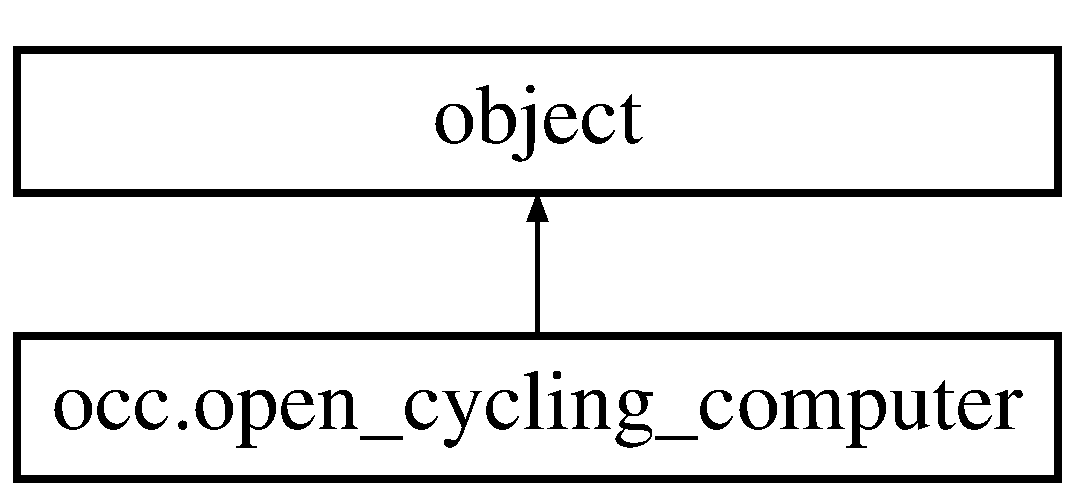
\includegraphics[height=2.000000cm]{classocc_1_1open__cycling__computer}
\end{center}
\end{figure}
\subsection*{Public Member Functions}
\begin{DoxyCompactItemize}
\item 
def \hyperlink{classocc_1_1open__cycling__computer_a1824c27f6e2c486c8b50f898db74d077}{\+\_\+\+\_\+init\+\_\+\+\_\+} (self, \hyperlink{classocc_1_1open__cycling__computer_a9bf952f2299899216b9adf8c382db024}{simulate}=False, \hyperlink{classocc_1_1open__cycling__computer_a56f3dab67d5bff0740ffbd8654d55582}{width}=240, \hyperlink{classocc_1_1open__cycling__computer_a2215795145291166265958493e692bab}{height}=320)
\begin{DoxyCompactList}\small\item\em The constructor. \end{DoxyCompactList}\item 
def \hyperlink{classocc_1_1open__cycling__computer_a4283facb6ffb6ed36e30bd9e3ed61871}{event\+\_\+iterator} (self)
\begin{DoxyCompactList}\small\item\em Provides events from pygame system. \end{DoxyCompactList}\item 
def \hyperlink{classocc_1_1open__cycling__computer_abff79cda8ca077b0bd319e08214dd6d3}{force\+\_\+refresh} (self)
\item 
def \hyperlink{classocc_1_1open__cycling__computer_a26649854452d1afcfebf0b3d17ac347d}{switch\+\_\+log\+\_\+level} (self, log\+\_\+level)
\begin{DoxyCompactList}\small\item\em Switches logging level. \end{DoxyCompactList}\item 
def \hyperlink{classocc_1_1open__cycling__computer_aea92ce48f815f4c3f3d56faab3ca025d}{screen\+\_\+touched\+\_\+handler} (self, time\+\_\+now)
\item 
def \hyperlink{classocc_1_1open__cycling__computer_a98a9ab4fb8dbd4df267ee216ef53d895}{event\+\_\+handler} (self, event, time\+\_\+now)
\item 
def \hyperlink{classocc_1_1open__cycling__computer_a6686554a1a2f2517d3ab46abb2bb35c2}{main\+\_\+loop} (self)
\item 
def \hyperlink{classocc_1_1open__cycling__computer_aa6adec92226434376a10fc852ebf6dc6}{reset\+\_\+motion} (self)
\item 
def \hyperlink{classocc_1_1open__cycling__computer_a1f6bf75367d3617a7b5c0e182c27e890}{cleanup} (self)
\end{DoxyCompactItemize}
\subsection*{Public Attributes}
\begin{DoxyCompactItemize}
\item 
\hyperlink{classocc_1_1open__cycling__computer_a9bf952f2299899216b9adf8c382db024}{simulate}
\begin{DoxyCompactList}\small\item\em Stores simulate parameter from constructor call. \end{DoxyCompactList}\item 
\hyperlink{classocc_1_1open__cycling__computer_ae6203e191770e28dde9a508a4d818dba}{l}
\begin{DoxyCompactList}\small\item\em Handle to system logger. \end{DoxyCompactList}\item 
\hyperlink{classocc_1_1open__cycling__computer_a56f3dab67d5bff0740ffbd8654d55582}{width}
\begin{DoxyCompactList}\small\item\em Window/screen width. \end{DoxyCompactList}\item 
\hyperlink{classocc_1_1open__cycling__computer_a2215795145291166265958493e692bab}{height}
\begin{DoxyCompactList}\small\item\em Window/screen height. \end{DoxyCompactList}\item 
\hyperlink{classocc_1_1open__cycling__computer_a6637c748b8ecbacd54bc36c504bfefaa}{screen}
\begin{DoxyCompactList}\small\item\em Handle to pygame screen. \end{DoxyCompactList}\item 
\hyperlink{classocc_1_1open__cycling__computer_a7fb670e84da1971f5b34c5f10e0b0418}{sensors}
\begin{DoxyCompactList}\small\item\em Handle to sensors instance. \end{DoxyCompactList}\item 
\hyperlink{classocc_1_1open__cycling__computer_afb5049a2519476feb5edd4fb6e4b2aea}{rp}
\begin{DoxyCompactList}\small\item\em Handle to \hyperlink{namespaceride__parameters}{ride\+\_\+parameters} instance. \end{DoxyCompactList}\item 
\hyperlink{classocc_1_1open__cycling__computer_a49c34e270f0d29f25f8ddb6ca1ee5631}{layout\+\_\+path}
\begin{DoxyCompactList}\small\item\em Path to layout file. \end{DoxyCompactList}\item 
\hyperlink{classocc_1_1open__cycling__computer_a9fcf030e68a44147a38f34d214572f44}{config}
\begin{DoxyCompactList}\small\item\em Handle to config instance. \end{DoxyCompactList}\item 
\hyperlink{classocc_1_1open__cycling__computer_ac8c629c48b3fff8add28a1c7f7fc31ca}{layout}
\begin{DoxyCompactList}\small\item\em Handle to layout instance. \end{DoxyCompactList}\item 
\hyperlink{classocc_1_1open__cycling__computer_a05f815f6c23686c9a9a7728b3808fc99}{rendering}
\begin{DoxyCompactList}\small\item\em Handle to rendering instance. \end{DoxyCompactList}\item 
\hyperlink{classocc_1_1open__cycling__computer_a63a6b256728b0d8ced4fbace9f43791d}{released\+\_\+t}
\begin{DoxyCompactList}\small\item\em Time stamp of pygame.\+M\+O\+U\+S\+E\+B\+U\+T\+T\+O\+N\+UP event (end of finger contact with touchscreen) \end{DoxyCompactList}\item 
\hyperlink{classocc_1_1open__cycling__computer_a1bbc11b7dd1d16fadc63aa7b6360f71d}{rel\+\_\+movement}
\begin{DoxyCompactList}\small\item\em Vector since M\+O\+U\+S\+E\+B\+U\+T\+T\+O\+N\+D\+O\+WN event. \end{DoxyCompactList}\item 
\hyperlink{classocc_1_1open__cycling__computer_a1ea38b7c9655b557eacce7dc377a9ce6}{pressed\+\_\+t}
\begin{DoxyCompactList}\small\item\em Time stamp of pygame.\+M\+O\+U\+S\+E\+B\+U\+T\+T\+O\+N\+D\+O\+WN event (start of finger contact with touchscreen) \end{DoxyCompactList}\item 
\hyperlink{classocc_1_1open__cycling__computer_aa57172c2a04bd0ff61e5dafdefe1554b}{pressed\+\_\+pos}
\begin{DoxyCompactList}\small\item\em Position of pygame.\+M\+O\+U\+S\+E\+B\+U\+T\+T\+O\+N\+D\+O\+WN event (start of finger contact with touchscreen) \end{DoxyCompactList}\item 
\hyperlink{classocc_1_1open__cycling__computer_a430f81b58f8be50077ebaa317d487812}{released\+\_\+pos}
\begin{DoxyCompactList}\small\item\em Position of pygame.\+M\+O\+U\+S\+E\+B\+U\+T\+T\+O\+N\+UP event (end of finger contact with touchscreen) \end{DoxyCompactList}\item 
\hyperlink{classocc_1_1open__cycling__computer_af56c12bbd4cf026b59578e22b922c846}{add\+\_\+rel\+\_\+motion}
\begin{DoxyCompactList}\small\item\em Used to control if finger/mouse vectors should be tracked to determine total relative motion. \end{DoxyCompactList}\item 
\hyperlink{classocc_1_1open__cycling__computer_ace5191a9d73e79fdba4ed1d9a7379274}{running}
\begin{DoxyCompactList}\small\item\em Variable controlling the main occ event loop. \end{DoxyCompactList}\item 
\hyperlink{classocc_1_1open__cycling__computer_a76ee74edfd950f99f8a52ae4fdcc3ac6}{refresh}
\begin{DoxyCompactList}\small\item\em Variable controlling if the screen need to be refreshed. \end{DoxyCompactList}\end{DoxyCompactItemize}


\subsection{Detailed Description}
Main O\+CC class. 

\subsection{Constructor \& Destructor Documentation}
\mbox{\Hypertarget{classocc_1_1open__cycling__computer_a1824c27f6e2c486c8b50f898db74d077}\label{classocc_1_1open__cycling__computer_a1824c27f6e2c486c8b50f898db74d077}} 
\index{occ\+::open\+\_\+cycling\+\_\+computer@{occ\+::open\+\_\+cycling\+\_\+computer}!\+\_\+\+\_\+init\+\_\+\+\_\+@{\+\_\+\+\_\+init\+\_\+\+\_\+}}
\index{\+\_\+\+\_\+init\+\_\+\+\_\+@{\+\_\+\+\_\+init\+\_\+\+\_\+}!occ\+::open\+\_\+cycling\+\_\+computer@{occ\+::open\+\_\+cycling\+\_\+computer}}
\subsubsection{\texorpdfstring{\+\_\+\+\_\+init\+\_\+\+\_\+()}{\_\_init\_\_()}}
{\footnotesize\ttfamily def occ.\+open\+\_\+cycling\+\_\+computer.\+\_\+\+\_\+init\+\_\+\+\_\+ (\begin{DoxyParamCaption}\item[{}]{self,  }\item[{}]{simulate = {\ttfamily False},  }\item[{}]{width = {\ttfamily 240},  }\item[{}]{height = {\ttfamily 320} }\end{DoxyParamCaption})}



The constructor. 


\begin{DoxyParams}{Parameters}
{\em self} & The python object self \\
\hline
{\em simulate} & Decides if O\+CC runs in simulation mode or real device mode. Simulation mode is useful for test on non-\/raspberry pi hardware. Default value is False. \\
\hline
{\em width} & Width of screen or window. Default value is 240 pixels \\
\hline
{\em height} & Height of screen or window. Default value is 320 pixels \\
\hline
\end{DoxyParams}


\subsection{Member Function Documentation}
\mbox{\Hypertarget{classocc_1_1open__cycling__computer_a1f6bf75367d3617a7b5c0e182c27e890}\label{classocc_1_1open__cycling__computer_a1f6bf75367d3617a7b5c0e182c27e890}} 
\index{occ\+::open\+\_\+cycling\+\_\+computer@{occ\+::open\+\_\+cycling\+\_\+computer}!cleanup@{cleanup}}
\index{cleanup@{cleanup}!occ\+::open\+\_\+cycling\+\_\+computer@{occ\+::open\+\_\+cycling\+\_\+computer}}
\subsubsection{\texorpdfstring{cleanup()}{cleanup()}}
{\footnotesize\ttfamily def occ.\+open\+\_\+cycling\+\_\+computer.\+cleanup (\begin{DoxyParamCaption}\item[{}]{self }\end{DoxyParamCaption})}

\mbox{\Hypertarget{classocc_1_1open__cycling__computer_a98a9ab4fb8dbd4df267ee216ef53d895}\label{classocc_1_1open__cycling__computer_a98a9ab4fb8dbd4df267ee216ef53d895}} 
\index{occ\+::open\+\_\+cycling\+\_\+computer@{occ\+::open\+\_\+cycling\+\_\+computer}!event\+\_\+handler@{event\+\_\+handler}}
\index{event\+\_\+handler@{event\+\_\+handler}!occ\+::open\+\_\+cycling\+\_\+computer@{occ\+::open\+\_\+cycling\+\_\+computer}}
\subsubsection{\texorpdfstring{event\+\_\+handler()}{event\_handler()}}
{\footnotesize\ttfamily def occ.\+open\+\_\+cycling\+\_\+computer.\+event\+\_\+handler (\begin{DoxyParamCaption}\item[{}]{self,  }\item[{}]{event,  }\item[{}]{time\+\_\+now }\end{DoxyParamCaption})}

\mbox{\Hypertarget{classocc_1_1open__cycling__computer_a4283facb6ffb6ed36e30bd9e3ed61871}\label{classocc_1_1open__cycling__computer_a4283facb6ffb6ed36e30bd9e3ed61871}} 
\index{occ\+::open\+\_\+cycling\+\_\+computer@{occ\+::open\+\_\+cycling\+\_\+computer}!event\+\_\+iterator@{event\+\_\+iterator}}
\index{event\+\_\+iterator@{event\+\_\+iterator}!occ\+::open\+\_\+cycling\+\_\+computer@{occ\+::open\+\_\+cycling\+\_\+computer}}
\subsubsection{\texorpdfstring{event\+\_\+iterator()}{event\_iterator()}}
{\footnotesize\ttfamily def occ.\+open\+\_\+cycling\+\_\+computer.\+event\+\_\+iterator (\begin{DoxyParamCaption}\item[{}]{self }\end{DoxyParamCaption})}



Provides events from pygame system. 


\begin{DoxyParams}{Parameters}
{\em self} & The python object self \\
\hline
\end{DoxyParams}
\mbox{\Hypertarget{classocc_1_1open__cycling__computer_abff79cda8ca077b0bd319e08214dd6d3}\label{classocc_1_1open__cycling__computer_abff79cda8ca077b0bd319e08214dd6d3}} 
\index{occ\+::open\+\_\+cycling\+\_\+computer@{occ\+::open\+\_\+cycling\+\_\+computer}!force\+\_\+refresh@{force\+\_\+refresh}}
\index{force\+\_\+refresh@{force\+\_\+refresh}!occ\+::open\+\_\+cycling\+\_\+computer@{occ\+::open\+\_\+cycling\+\_\+computer}}
\subsubsection{\texorpdfstring{force\+\_\+refresh()}{force\_refresh()}}
{\footnotesize\ttfamily def occ.\+open\+\_\+cycling\+\_\+computer.\+force\+\_\+refresh (\begin{DoxyParamCaption}\item[{}]{self }\end{DoxyParamCaption})}

\mbox{\Hypertarget{classocc_1_1open__cycling__computer_a6686554a1a2f2517d3ab46abb2bb35c2}\label{classocc_1_1open__cycling__computer_a6686554a1a2f2517d3ab46abb2bb35c2}} 
\index{occ\+::open\+\_\+cycling\+\_\+computer@{occ\+::open\+\_\+cycling\+\_\+computer}!main\+\_\+loop@{main\+\_\+loop}}
\index{main\+\_\+loop@{main\+\_\+loop}!occ\+::open\+\_\+cycling\+\_\+computer@{occ\+::open\+\_\+cycling\+\_\+computer}}
\subsubsection{\texorpdfstring{main\+\_\+loop()}{main\_loop()}}
{\footnotesize\ttfamily def occ.\+open\+\_\+cycling\+\_\+computer.\+main\+\_\+loop (\begin{DoxyParamCaption}\item[{}]{self }\end{DoxyParamCaption})}

\mbox{\Hypertarget{classocc_1_1open__cycling__computer_aa6adec92226434376a10fc852ebf6dc6}\label{classocc_1_1open__cycling__computer_aa6adec92226434376a10fc852ebf6dc6}} 
\index{occ\+::open\+\_\+cycling\+\_\+computer@{occ\+::open\+\_\+cycling\+\_\+computer}!reset\+\_\+motion@{reset\+\_\+motion}}
\index{reset\+\_\+motion@{reset\+\_\+motion}!occ\+::open\+\_\+cycling\+\_\+computer@{occ\+::open\+\_\+cycling\+\_\+computer}}
\subsubsection{\texorpdfstring{reset\+\_\+motion()}{reset\_motion()}}
{\footnotesize\ttfamily def occ.\+open\+\_\+cycling\+\_\+computer.\+reset\+\_\+motion (\begin{DoxyParamCaption}\item[{}]{self }\end{DoxyParamCaption})}

\mbox{\Hypertarget{classocc_1_1open__cycling__computer_aea92ce48f815f4c3f3d56faab3ca025d}\label{classocc_1_1open__cycling__computer_aea92ce48f815f4c3f3d56faab3ca025d}} 
\index{occ\+::open\+\_\+cycling\+\_\+computer@{occ\+::open\+\_\+cycling\+\_\+computer}!screen\+\_\+touched\+\_\+handler@{screen\+\_\+touched\+\_\+handler}}
\index{screen\+\_\+touched\+\_\+handler@{screen\+\_\+touched\+\_\+handler}!occ\+::open\+\_\+cycling\+\_\+computer@{occ\+::open\+\_\+cycling\+\_\+computer}}
\subsubsection{\texorpdfstring{screen\+\_\+touched\+\_\+handler()}{screen\_touched\_handler()}}
{\footnotesize\ttfamily def occ.\+open\+\_\+cycling\+\_\+computer.\+screen\+\_\+touched\+\_\+handler (\begin{DoxyParamCaption}\item[{}]{self,  }\item[{}]{time\+\_\+now }\end{DoxyParamCaption})}

\mbox{\Hypertarget{classocc_1_1open__cycling__computer_a26649854452d1afcfebf0b3d17ac347d}\label{classocc_1_1open__cycling__computer_a26649854452d1afcfebf0b3d17ac347d}} 
\index{occ\+::open\+\_\+cycling\+\_\+computer@{occ\+::open\+\_\+cycling\+\_\+computer}!switch\+\_\+log\+\_\+level@{switch\+\_\+log\+\_\+level}}
\index{switch\+\_\+log\+\_\+level@{switch\+\_\+log\+\_\+level}!occ\+::open\+\_\+cycling\+\_\+computer@{occ\+::open\+\_\+cycling\+\_\+computer}}
\subsubsection{\texorpdfstring{switch\+\_\+log\+\_\+level()}{switch\_log\_level()}}
{\footnotesize\ttfamily def occ.\+open\+\_\+cycling\+\_\+computer.\+switch\+\_\+log\+\_\+level (\begin{DoxyParamCaption}\item[{}]{self,  }\item[{}]{log\+\_\+level }\end{DoxyParamCaption})}



Switches logging level. 


\begin{DoxyParams}{Parameters}
{\em self} & The python object self \\
\hline
{\em log\+\_\+level} & Log level to be set. Allowed levels are in \hyperlink{namespaceocc_a46db66163eeb50234471c2f1f0bf4133}{L\+O\+G\+\_\+\+L\+E\+V\+EL} \\
\hline
\end{DoxyParams}


\subsection{Member Data Documentation}
\mbox{\Hypertarget{classocc_1_1open__cycling__computer_af56c12bbd4cf026b59578e22b922c846}\label{classocc_1_1open__cycling__computer_af56c12bbd4cf026b59578e22b922c846}} 
\index{occ\+::open\+\_\+cycling\+\_\+computer@{occ\+::open\+\_\+cycling\+\_\+computer}!add\+\_\+rel\+\_\+motion@{add\+\_\+rel\+\_\+motion}}
\index{add\+\_\+rel\+\_\+motion@{add\+\_\+rel\+\_\+motion}!occ\+::open\+\_\+cycling\+\_\+computer@{occ\+::open\+\_\+cycling\+\_\+computer}}
\subsubsection{\texorpdfstring{add\+\_\+rel\+\_\+motion}{add\_rel\_motion}}
{\footnotesize\ttfamily occ.\+open\+\_\+cycling\+\_\+computer.\+add\+\_\+rel\+\_\+motion}



Used to control if finger/mouse vectors should be tracked to determine total relative motion. 

\mbox{\Hypertarget{classocc_1_1open__cycling__computer_a9fcf030e68a44147a38f34d214572f44}\label{classocc_1_1open__cycling__computer_a9fcf030e68a44147a38f34d214572f44}} 
\index{occ\+::open\+\_\+cycling\+\_\+computer@{occ\+::open\+\_\+cycling\+\_\+computer}!config@{config}}
\index{config@{config}!occ\+::open\+\_\+cycling\+\_\+computer@{occ\+::open\+\_\+cycling\+\_\+computer}}
\subsubsection{\texorpdfstring{config}{config}}
{\footnotesize\ttfamily occ.\+open\+\_\+cycling\+\_\+computer.\+config}



Handle to config instance. 

\mbox{\Hypertarget{classocc_1_1open__cycling__computer_a2215795145291166265958493e692bab}\label{classocc_1_1open__cycling__computer_a2215795145291166265958493e692bab}} 
\index{occ\+::open\+\_\+cycling\+\_\+computer@{occ\+::open\+\_\+cycling\+\_\+computer}!height@{height}}
\index{height@{height}!occ\+::open\+\_\+cycling\+\_\+computer@{occ\+::open\+\_\+cycling\+\_\+computer}}
\subsubsection{\texorpdfstring{height}{height}}
{\footnotesize\ttfamily occ.\+open\+\_\+cycling\+\_\+computer.\+height}



Window/screen height. 

\mbox{\Hypertarget{classocc_1_1open__cycling__computer_ae6203e191770e28dde9a508a4d818dba}\label{classocc_1_1open__cycling__computer_ae6203e191770e28dde9a508a4d818dba}} 
\index{occ\+::open\+\_\+cycling\+\_\+computer@{occ\+::open\+\_\+cycling\+\_\+computer}!l@{l}}
\index{l@{l}!occ\+::open\+\_\+cycling\+\_\+computer@{occ\+::open\+\_\+cycling\+\_\+computer}}
\subsubsection{\texorpdfstring{l}{l}}
{\footnotesize\ttfamily occ.\+open\+\_\+cycling\+\_\+computer.\+l}



Handle to system logger. 

\mbox{\Hypertarget{classocc_1_1open__cycling__computer_ac8c629c48b3fff8add28a1c7f7fc31ca}\label{classocc_1_1open__cycling__computer_ac8c629c48b3fff8add28a1c7f7fc31ca}} 
\index{occ\+::open\+\_\+cycling\+\_\+computer@{occ\+::open\+\_\+cycling\+\_\+computer}!layout@{layout}}
\index{layout@{layout}!occ\+::open\+\_\+cycling\+\_\+computer@{occ\+::open\+\_\+cycling\+\_\+computer}}
\subsubsection{\texorpdfstring{layout}{layout}}
{\footnotesize\ttfamily occ.\+open\+\_\+cycling\+\_\+computer.\+layout}



Handle to layout instance. 

\mbox{\Hypertarget{classocc_1_1open__cycling__computer_a49c34e270f0d29f25f8ddb6ca1ee5631}\label{classocc_1_1open__cycling__computer_a49c34e270f0d29f25f8ddb6ca1ee5631}} 
\index{occ\+::open\+\_\+cycling\+\_\+computer@{occ\+::open\+\_\+cycling\+\_\+computer}!layout\+\_\+path@{layout\+\_\+path}}
\index{layout\+\_\+path@{layout\+\_\+path}!occ\+::open\+\_\+cycling\+\_\+computer@{occ\+::open\+\_\+cycling\+\_\+computer}}
\subsubsection{\texorpdfstring{layout\+\_\+path}{layout\_path}}
{\footnotesize\ttfamily occ.\+open\+\_\+cycling\+\_\+computer.\+layout\+\_\+path}



Path to layout file. 

\mbox{\Hypertarget{classocc_1_1open__cycling__computer_aa57172c2a04bd0ff61e5dafdefe1554b}\label{classocc_1_1open__cycling__computer_aa57172c2a04bd0ff61e5dafdefe1554b}} 
\index{occ\+::open\+\_\+cycling\+\_\+computer@{occ\+::open\+\_\+cycling\+\_\+computer}!pressed\+\_\+pos@{pressed\+\_\+pos}}
\index{pressed\+\_\+pos@{pressed\+\_\+pos}!occ\+::open\+\_\+cycling\+\_\+computer@{occ\+::open\+\_\+cycling\+\_\+computer}}
\subsubsection{\texorpdfstring{pressed\+\_\+pos}{pressed\_pos}}
{\footnotesize\ttfamily occ.\+open\+\_\+cycling\+\_\+computer.\+pressed\+\_\+pos}



Position of pygame.\+M\+O\+U\+S\+E\+B\+U\+T\+T\+O\+N\+D\+O\+WN event (start of finger contact with touchscreen) 

\mbox{\Hypertarget{classocc_1_1open__cycling__computer_a1ea38b7c9655b557eacce7dc377a9ce6}\label{classocc_1_1open__cycling__computer_a1ea38b7c9655b557eacce7dc377a9ce6}} 
\index{occ\+::open\+\_\+cycling\+\_\+computer@{occ\+::open\+\_\+cycling\+\_\+computer}!pressed\+\_\+t@{pressed\+\_\+t}}
\index{pressed\+\_\+t@{pressed\+\_\+t}!occ\+::open\+\_\+cycling\+\_\+computer@{occ\+::open\+\_\+cycling\+\_\+computer}}
\subsubsection{\texorpdfstring{pressed\+\_\+t}{pressed\_t}}
{\footnotesize\ttfamily occ.\+open\+\_\+cycling\+\_\+computer.\+pressed\+\_\+t}



Time stamp of pygame.\+M\+O\+U\+S\+E\+B\+U\+T\+T\+O\+N\+D\+O\+WN event (start of finger contact with touchscreen) 

\mbox{\Hypertarget{classocc_1_1open__cycling__computer_a76ee74edfd950f99f8a52ae4fdcc3ac6}\label{classocc_1_1open__cycling__computer_a76ee74edfd950f99f8a52ae4fdcc3ac6}} 
\index{occ\+::open\+\_\+cycling\+\_\+computer@{occ\+::open\+\_\+cycling\+\_\+computer}!refresh@{refresh}}
\index{refresh@{refresh}!occ\+::open\+\_\+cycling\+\_\+computer@{occ\+::open\+\_\+cycling\+\_\+computer}}
\subsubsection{\texorpdfstring{refresh}{refresh}}
{\footnotesize\ttfamily occ.\+open\+\_\+cycling\+\_\+computer.\+refresh}



Variable controlling if the screen need to be refreshed. 

\mbox{\Hypertarget{classocc_1_1open__cycling__computer_a1bbc11b7dd1d16fadc63aa7b6360f71d}\label{classocc_1_1open__cycling__computer_a1bbc11b7dd1d16fadc63aa7b6360f71d}} 
\index{occ\+::open\+\_\+cycling\+\_\+computer@{occ\+::open\+\_\+cycling\+\_\+computer}!rel\+\_\+movement@{rel\+\_\+movement}}
\index{rel\+\_\+movement@{rel\+\_\+movement}!occ\+::open\+\_\+cycling\+\_\+computer@{occ\+::open\+\_\+cycling\+\_\+computer}}
\subsubsection{\texorpdfstring{rel\+\_\+movement}{rel\_movement}}
{\footnotesize\ttfamily occ.\+open\+\_\+cycling\+\_\+computer.\+rel\+\_\+movement}



Vector since M\+O\+U\+S\+E\+B\+U\+T\+T\+O\+N\+D\+O\+WN event. 

Used to derermine swipe motion. \mbox{\Hypertarget{classocc_1_1open__cycling__computer_a430f81b58f8be50077ebaa317d487812}\label{classocc_1_1open__cycling__computer_a430f81b58f8be50077ebaa317d487812}} 
\index{occ\+::open\+\_\+cycling\+\_\+computer@{occ\+::open\+\_\+cycling\+\_\+computer}!released\+\_\+pos@{released\+\_\+pos}}
\index{released\+\_\+pos@{released\+\_\+pos}!occ\+::open\+\_\+cycling\+\_\+computer@{occ\+::open\+\_\+cycling\+\_\+computer}}
\subsubsection{\texorpdfstring{released\+\_\+pos}{released\_pos}}
{\footnotesize\ttfamily occ.\+open\+\_\+cycling\+\_\+computer.\+released\+\_\+pos}



Position of pygame.\+M\+O\+U\+S\+E\+B\+U\+T\+T\+O\+N\+UP event (end of finger contact with touchscreen) 

\mbox{\Hypertarget{classocc_1_1open__cycling__computer_a63a6b256728b0d8ced4fbace9f43791d}\label{classocc_1_1open__cycling__computer_a63a6b256728b0d8ced4fbace9f43791d}} 
\index{occ\+::open\+\_\+cycling\+\_\+computer@{occ\+::open\+\_\+cycling\+\_\+computer}!released\+\_\+t@{released\+\_\+t}}
\index{released\+\_\+t@{released\+\_\+t}!occ\+::open\+\_\+cycling\+\_\+computer@{occ\+::open\+\_\+cycling\+\_\+computer}}
\subsubsection{\texorpdfstring{released\+\_\+t}{released\_t}}
{\footnotesize\ttfamily occ.\+open\+\_\+cycling\+\_\+computer.\+released\+\_\+t}



Time stamp of pygame.\+M\+O\+U\+S\+E\+B\+U\+T\+T\+O\+N\+UP event (end of finger contact with touchscreen) 

\mbox{\Hypertarget{classocc_1_1open__cycling__computer_a05f815f6c23686c9a9a7728b3808fc99}\label{classocc_1_1open__cycling__computer_a05f815f6c23686c9a9a7728b3808fc99}} 
\index{occ\+::open\+\_\+cycling\+\_\+computer@{occ\+::open\+\_\+cycling\+\_\+computer}!rendering@{rendering}}
\index{rendering@{rendering}!occ\+::open\+\_\+cycling\+\_\+computer@{occ\+::open\+\_\+cycling\+\_\+computer}}
\subsubsection{\texorpdfstring{rendering}{rendering}}
{\footnotesize\ttfamily occ.\+open\+\_\+cycling\+\_\+computer.\+rendering}



Handle to rendering instance. 

\mbox{\Hypertarget{classocc_1_1open__cycling__computer_afb5049a2519476feb5edd4fb6e4b2aea}\label{classocc_1_1open__cycling__computer_afb5049a2519476feb5edd4fb6e4b2aea}} 
\index{occ\+::open\+\_\+cycling\+\_\+computer@{occ\+::open\+\_\+cycling\+\_\+computer}!rp@{rp}}
\index{rp@{rp}!occ\+::open\+\_\+cycling\+\_\+computer@{occ\+::open\+\_\+cycling\+\_\+computer}}
\subsubsection{\texorpdfstring{rp}{rp}}
{\footnotesize\ttfamily occ.\+open\+\_\+cycling\+\_\+computer.\+rp}



Handle to \hyperlink{namespaceride__parameters}{ride\+\_\+parameters} instance. 

\mbox{\Hypertarget{classocc_1_1open__cycling__computer_ace5191a9d73e79fdba4ed1d9a7379274}\label{classocc_1_1open__cycling__computer_ace5191a9d73e79fdba4ed1d9a7379274}} 
\index{occ\+::open\+\_\+cycling\+\_\+computer@{occ\+::open\+\_\+cycling\+\_\+computer}!running@{running}}
\index{running@{running}!occ\+::open\+\_\+cycling\+\_\+computer@{occ\+::open\+\_\+cycling\+\_\+computer}}
\subsubsection{\texorpdfstring{running}{running}}
{\footnotesize\ttfamily occ.\+open\+\_\+cycling\+\_\+computer.\+running}



Variable controlling the main occ event loop. 

pygame.\+Q\+U\+IT event triggers setting running to False \mbox{\Hypertarget{classocc_1_1open__cycling__computer_a6637c748b8ecbacd54bc36c504bfefaa}\label{classocc_1_1open__cycling__computer_a6637c748b8ecbacd54bc36c504bfefaa}} 
\index{occ\+::open\+\_\+cycling\+\_\+computer@{occ\+::open\+\_\+cycling\+\_\+computer}!screen@{screen}}
\index{screen@{screen}!occ\+::open\+\_\+cycling\+\_\+computer@{occ\+::open\+\_\+cycling\+\_\+computer}}
\subsubsection{\texorpdfstring{screen}{screen}}
{\footnotesize\ttfamily occ.\+open\+\_\+cycling\+\_\+computer.\+screen}



Handle to pygame screen. 

\mbox{\Hypertarget{classocc_1_1open__cycling__computer_a7fb670e84da1971f5b34c5f10e0b0418}\label{classocc_1_1open__cycling__computer_a7fb670e84da1971f5b34c5f10e0b0418}} 
\index{occ\+::open\+\_\+cycling\+\_\+computer@{occ\+::open\+\_\+cycling\+\_\+computer}!sensors@{sensors}}
\index{sensors@{sensors}!occ\+::open\+\_\+cycling\+\_\+computer@{occ\+::open\+\_\+cycling\+\_\+computer}}
\subsubsection{\texorpdfstring{sensors}{sensors}}
{\footnotesize\ttfamily occ.\+open\+\_\+cycling\+\_\+computer.\+sensors}



Handle to sensors instance. 

\mbox{\Hypertarget{classocc_1_1open__cycling__computer_a9bf952f2299899216b9adf8c382db024}\label{classocc_1_1open__cycling__computer_a9bf952f2299899216b9adf8c382db024}} 
\index{occ\+::open\+\_\+cycling\+\_\+computer@{occ\+::open\+\_\+cycling\+\_\+computer}!simulate@{simulate}}
\index{simulate@{simulate}!occ\+::open\+\_\+cycling\+\_\+computer@{occ\+::open\+\_\+cycling\+\_\+computer}}
\subsubsection{\texorpdfstring{simulate}{simulate}}
{\footnotesize\ttfamily occ.\+open\+\_\+cycling\+\_\+computer.\+simulate}



Stores simulate parameter from constructor call. 

\mbox{\Hypertarget{classocc_1_1open__cycling__computer_a56f3dab67d5bff0740ffbd8654d55582}\label{classocc_1_1open__cycling__computer_a56f3dab67d5bff0740ffbd8654d55582}} 
\index{occ\+::open\+\_\+cycling\+\_\+computer@{occ\+::open\+\_\+cycling\+\_\+computer}!width@{width}}
\index{width@{width}!occ\+::open\+\_\+cycling\+\_\+computer@{occ\+::open\+\_\+cycling\+\_\+computer}}
\subsubsection{\texorpdfstring{width}{width}}
{\footnotesize\ttfamily occ.\+open\+\_\+cycling\+\_\+computer.\+width}



Window/screen width. 



The documentation for this class was generated from the following file\+:\begin{DoxyCompactItemize}
\item 
src/\hyperlink{occ_8py}{occ.\+py}\end{DoxyCompactItemize}

\hypertarget{classrendering_1_1rendering}{}\section{rendering.\+rendering Class Reference}
\label{classrendering_1_1rendering}\index{rendering.\+rendering@{rendering.\+rendering}}
Inheritance diagram for rendering.\+rendering\+:\begin{figure}[H]
\begin{center}
\leavevmode
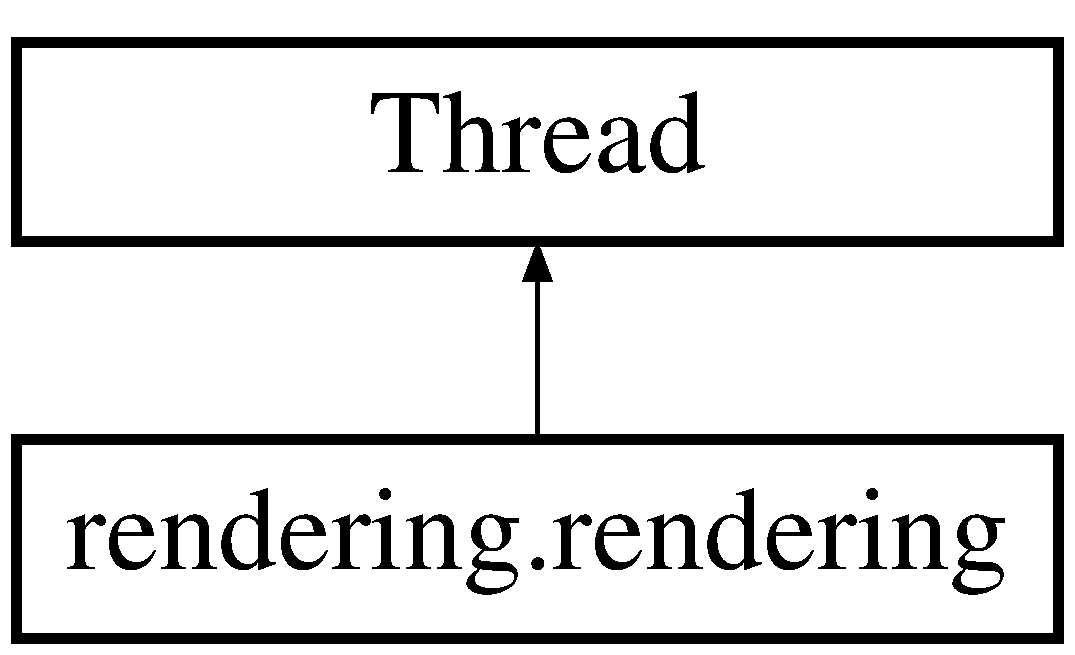
\includegraphics[height=2.000000cm]{classrendering_1_1rendering}
\end{center}
\end{figure}
\subsection*{Public Member Functions}
\begin{DoxyCompactItemize}
\item 
def \hyperlink{classrendering_1_1rendering_ac5379553b476c1582ac0d46421f215cb}{\+\_\+\+\_\+init\+\_\+\+\_\+} (self, \hyperlink{classrendering_1_1rendering_ae24d971b9a3addeac990b60abe4be00c}{layout})
\item 
def \hyperlink{classrendering_1_1rendering_a3116ee6b43720cc46180929920e837fc}{run} (self)
\item 
def \hyperlink{classrendering_1_1rendering_a7a5eff668345f94690e0737624416432}{stop} (self)
\item 
def \hyperlink{classrendering_1_1rendering_a2a20df6fdb79fdb9bbd16319ba02b631}{force\+\_\+refresh} (self)
\item 
def \hyperlink{classrendering_1_1rendering_a7a953f9a342455faaed5789eeca27419}{\+\_\+\+\_\+del\+\_\+\+\_\+} (self)
\end{DoxyCompactItemize}
\subsection*{Public Attributes}
\begin{DoxyCompactItemize}
\item 
\hyperlink{classrendering_1_1rendering_a209763b3162b34173314ab6ef43891cc}{clock}
\item 
\hyperlink{classrendering_1_1rendering_ae24d971b9a3addeac990b60abe4be00c}{layout}
\item 
\hyperlink{classrendering_1_1rendering_a7060a1797d07abb18e5eec51faeef313}{refresh}
\item 
\hyperlink{classrendering_1_1rendering_accfbd0ead30cf813505a94daf4a193df}{running}
\end{DoxyCompactItemize}


\subsection{Constructor \& Destructor Documentation}
\mbox{\Hypertarget{classrendering_1_1rendering_ac5379553b476c1582ac0d46421f215cb}\label{classrendering_1_1rendering_ac5379553b476c1582ac0d46421f215cb}} 
\index{rendering\+::rendering@{rendering\+::rendering}!\+\_\+\+\_\+init\+\_\+\+\_\+@{\+\_\+\+\_\+init\+\_\+\+\_\+}}
\index{\+\_\+\+\_\+init\+\_\+\+\_\+@{\+\_\+\+\_\+init\+\_\+\+\_\+}!rendering\+::rendering@{rendering\+::rendering}}
\subsubsection{\texorpdfstring{\+\_\+\+\_\+init\+\_\+\+\_\+()}{\_\_init\_\_()}}
{\footnotesize\ttfamily def rendering.\+rendering.\+\_\+\+\_\+init\+\_\+\+\_\+ (\begin{DoxyParamCaption}\item[{}]{self,  }\item[{}]{layout }\end{DoxyParamCaption})}

\mbox{\Hypertarget{classrendering_1_1rendering_a7a953f9a342455faaed5789eeca27419}\label{classrendering_1_1rendering_a7a953f9a342455faaed5789eeca27419}} 
\index{rendering\+::rendering@{rendering\+::rendering}!\+\_\+\+\_\+del\+\_\+\+\_\+@{\+\_\+\+\_\+del\+\_\+\+\_\+}}
\index{\+\_\+\+\_\+del\+\_\+\+\_\+@{\+\_\+\+\_\+del\+\_\+\+\_\+}!rendering\+::rendering@{rendering\+::rendering}}
\subsubsection{\texorpdfstring{\+\_\+\+\_\+del\+\_\+\+\_\+()}{\_\_del\_\_()}}
{\footnotesize\ttfamily def rendering.\+rendering.\+\_\+\+\_\+del\+\_\+\+\_\+ (\begin{DoxyParamCaption}\item[{}]{self }\end{DoxyParamCaption})}



\subsection{Member Function Documentation}
\mbox{\Hypertarget{classrendering_1_1rendering_a2a20df6fdb79fdb9bbd16319ba02b631}\label{classrendering_1_1rendering_a2a20df6fdb79fdb9bbd16319ba02b631}} 
\index{rendering\+::rendering@{rendering\+::rendering}!force\+\_\+refresh@{force\+\_\+refresh}}
\index{force\+\_\+refresh@{force\+\_\+refresh}!rendering\+::rendering@{rendering\+::rendering}}
\subsubsection{\texorpdfstring{force\+\_\+refresh()}{force\_refresh()}}
{\footnotesize\ttfamily def rendering.\+rendering.\+force\+\_\+refresh (\begin{DoxyParamCaption}\item[{}]{self }\end{DoxyParamCaption})}

\mbox{\Hypertarget{classrendering_1_1rendering_a3116ee6b43720cc46180929920e837fc}\label{classrendering_1_1rendering_a3116ee6b43720cc46180929920e837fc}} 
\index{rendering\+::rendering@{rendering\+::rendering}!run@{run}}
\index{run@{run}!rendering\+::rendering@{rendering\+::rendering}}
\subsubsection{\texorpdfstring{run()}{run()}}
{\footnotesize\ttfamily def rendering.\+rendering.\+run (\begin{DoxyParamCaption}\item[{}]{self }\end{DoxyParamCaption})}

\mbox{\Hypertarget{classrendering_1_1rendering_a7a5eff668345f94690e0737624416432}\label{classrendering_1_1rendering_a7a5eff668345f94690e0737624416432}} 
\index{rendering\+::rendering@{rendering\+::rendering}!stop@{stop}}
\index{stop@{stop}!rendering\+::rendering@{rendering\+::rendering}}
\subsubsection{\texorpdfstring{stop()}{stop()}}
{\footnotesize\ttfamily def rendering.\+rendering.\+stop (\begin{DoxyParamCaption}\item[{}]{self }\end{DoxyParamCaption})}



\subsection{Member Data Documentation}
\mbox{\Hypertarget{classrendering_1_1rendering_a209763b3162b34173314ab6ef43891cc}\label{classrendering_1_1rendering_a209763b3162b34173314ab6ef43891cc}} 
\index{rendering\+::rendering@{rendering\+::rendering}!clock@{clock}}
\index{clock@{clock}!rendering\+::rendering@{rendering\+::rendering}}
\subsubsection{\texorpdfstring{clock}{clock}}
{\footnotesize\ttfamily rendering.\+rendering.\+clock}

\mbox{\Hypertarget{classrendering_1_1rendering_ae24d971b9a3addeac990b60abe4be00c}\label{classrendering_1_1rendering_ae24d971b9a3addeac990b60abe4be00c}} 
\index{rendering\+::rendering@{rendering\+::rendering}!layout@{layout}}
\index{layout@{layout}!rendering\+::rendering@{rendering\+::rendering}}
\subsubsection{\texorpdfstring{layout}{layout}}
{\footnotesize\ttfamily rendering.\+rendering.\+layout}

\mbox{\Hypertarget{classrendering_1_1rendering_a7060a1797d07abb18e5eec51faeef313}\label{classrendering_1_1rendering_a7060a1797d07abb18e5eec51faeef313}} 
\index{rendering\+::rendering@{rendering\+::rendering}!refresh@{refresh}}
\index{refresh@{refresh}!rendering\+::rendering@{rendering\+::rendering}}
\subsubsection{\texorpdfstring{refresh}{refresh}}
{\footnotesize\ttfamily rendering.\+rendering.\+refresh}

\mbox{\Hypertarget{classrendering_1_1rendering_accfbd0ead30cf813505a94daf4a193df}\label{classrendering_1_1rendering_accfbd0ead30cf813505a94daf4a193df}} 
\index{rendering\+::rendering@{rendering\+::rendering}!running@{running}}
\index{running@{running}!rendering\+::rendering@{rendering\+::rendering}}
\subsubsection{\texorpdfstring{running}{running}}
{\footnotesize\ttfamily rendering.\+rendering.\+running}



The documentation for this class was generated from the following file\+:\begin{DoxyCompactItemize}
\item 
src/\hyperlink{rendering_8py}{rendering.\+py}\end{DoxyCompactItemize}

\hypertarget{classride__parameters_1_1ride__parameters}{}\section{ride\+\_\+parameters.\+ride\+\_\+parameters Class Reference}
\label{classride__parameters_1_1ride__parameters}\index{ride\+\_\+parameters.\+ride\+\_\+parameters@{ride\+\_\+parameters.\+ride\+\_\+parameters}}
\subsection*{Public Member Functions}
\begin{DoxyCompactItemize}
\item 
def \hyperlink{classride__parameters_1_1ride__parameters_a2b6d7ea51b7ceb4cda0370a00028e048}{\+\_\+\+\_\+init\+\_\+\+\_\+} (self, \hyperlink{classride__parameters_1_1ride__parameters_a76014d9517093d35d2660f8660544071}{occ}, simulate=False)
\item 
def \hyperlink{classride__parameters_1_1ride__parameters_afce46ab54897c7bfb53dfc41369ea710}{start\+\_\+sensors} (self)
\item 
def \hyperlink{classride__parameters_1_1ride__parameters_a28fd2385edb5031e2ed4ef601707f78b}{setup\+\_\+ridelog} (self)
\item 
def \hyperlink{classride__parameters_1_1ride__parameters_a38286161b1fed8db1a1eab4f72bc100d}{stop} (self)
\item 
def \hyperlink{classride__parameters_1_1ride__parameters_ac7565bcad12b1d5c16d14fa1dd93b600}{\+\_\+\+\_\+del\+\_\+\+\_\+} (self)
\item 
def \hyperlink{classride__parameters_1_1ride__parameters_a0298eab61d08a06ce19b02a7a2017261}{update\+\_\+values} (self)
\item 
def \hyperlink{classride__parameters_1_1ride__parameters_a5a52f0de392b339a4645f5a6b7f5c028}{calculate\+\_\+time\+\_\+related\+\_\+parameters} (self)
\item 
def \hyperlink{classride__parameters_1_1ride__parameters_abdbe40847a9540e6fbea1aa1c395f4c0}{force\+\_\+refresh} (self)
\item 
def \hyperlink{classride__parameters_1_1ride__parameters_aca8aefb88a0260ec04ea182a9331facd}{get\+\_\+raw\+\_\+val} (self, param)
\item 
def \hyperlink{classride__parameters_1_1ride__parameters_a9dc6e4ca486f38f6b26953427ef0586b}{set\+\_\+param} (self, param\+\_\+name, value)
\item 
def \hyperlink{classride__parameters_1_1ride__parameters_aeb3f33542ac30687ce80dac161fcd193}{get\+\_\+param} (self, param)
\item 
def \hyperlink{classride__parameters_1_1ride__parameters_a8108dcab38d0a57e363da69ce383038e}{get\+\_\+unit} (self, param\+\_\+name)
\item 
def \hyperlink{classride__parameters_1_1ride__parameters_a5f1472b2156773cecd43da4ade606fd1}{get\+\_\+internal\+\_\+unit} (self, param\+\_\+name)
\item 
def \hyperlink{classride__parameters_1_1ride__parameters_a3fd3198dfcd50bbcafcaac194339e3a5}{get\+\_\+description} (self, param\+\_\+name)
\item 
def \hyperlink{classride__parameters_1_1ride__parameters_ac05416d0080d15decb714bdbd68dfeef}{clean\+\_\+value} (self, variable, empty=0)
\item 
def \hyperlink{classride__parameters_1_1ride__parameters_a41a11edd11c4c3088597ef48583fe5ec}{read\+\_\+ble\+\_\+data} (self)
\item 
def \hyperlink{classride__parameters_1_1ride__parameters_a7b3691fb41527f59f5d2bb1b537d842d}{read\+\_\+gps\+\_\+data} (self)
\item 
def \hyperlink{classride__parameters_1_1ride__parameters_ac92ac15cba00fe7c440cb887966ad9ae}{split\+\_\+speed} (self, speed\+\_\+name)
\item 
def \hyperlink{classride__parameters_1_1ride__parameters_a18c56686f5b82a73482130fbaadc9bc7}{update\+\_\+max\+\_\+speed} (self)
\item 
def \hyperlink{classride__parameters_1_1ride__parameters_a9807fc1da341854145ce767ab5c30a03}{update\+\_\+fix\+\_\+gps} (self)
\item 
def \hyperlink{classride__parameters_1_1ride__parameters_aa9a8380985766a4055005d900d4ba88c}{set\+\_\+max} (self, param)
\item 
def \hyperlink{classride__parameters_1_1ride__parameters_a158b11d8e0c003428a576925a1bc3a06}{set\+\_\+min} (self, param)
\item 
def \hyperlink{classride__parameters_1_1ride__parameters_a1e1f51a19a57e25581e7c68bdc223220}{calculate\+\_\+avg\+\_\+temperature} (self)
\item 
def \hyperlink{classride__parameters_1_1ride__parameters_a118d405141974f9cdd157c99632750e7}{calculate\+\_\+avg\+\_\+cadence} (self)
\item 
def \hyperlink{classride__parameters_1_1ride__parameters_a7cdd705426c5a6b3e14c84d6ca4e8315}{calculate\+\_\+avg\+\_\+heart\+\_\+rate} (self)
\item 
def \hyperlink{classride__parameters_1_1ride__parameters_ac43553319b5a7bf338055b4a4e7ad6f8}{update\+\_\+altitude} (self)
\item 
def \hyperlink{classride__parameters_1_1ride__parameters_ae69dbac396ca79bc9f00d68c5acd2150}{update\+\_\+params} (self)
\item 
def \hyperlink{classride__parameters_1_1ride__parameters_ad0d886eb956cb3bcb8be953e03e6dab6}{add\+\_\+ridelog\+\_\+entry} (self)
\item 
def \hyperlink{classride__parameters_1_1ride__parameters_a5d2ad4b83bce4e8391cf0d702304686f}{strip\+\_\+end} (self, param\+\_\+name, suffix=None)
\item 
def \hyperlink{classride__parameters_1_1ride__parameters_a36178e22c36591cb24b08974e5123f27}{reset\+\_\+ride} (self)
\item 
def \hyperlink{classride__parameters_1_1ride__parameters_a8aab50a51a67d682e97834e178996d12}{reset\+\_\+cadence} (self)
\item 
def \hyperlink{classride__parameters_1_1ride__parameters_a41f168d7dcd81c7be64f104cabc9c84a}{reset\+\_\+heart\+\_\+rate} (self)
\item 
def \hyperlink{classride__parameters_1_1ride__parameters_acdb03382d51f8c03d4e0dbe347ddadb4}{reset\+\_\+param} (self, param\+\_\+name)
\item 
def \hyperlink{classride__parameters_1_1ride__parameters_ab01d91e41b6d2941f3d00905d29d3d23}{update\+\_\+param} (self, param\+\_\+name)
\item 
def \hyperlink{classride__parameters_1_1ride__parameters_a1bb15203890685c84d01ea5d37fe187b}{add\+\_\+zero} (self, value)
\item 
def \hyperlink{classride__parameters_1_1ride__parameters_aa74512ad30be2ec2784970e652649e93}{update\+\_\+hms} (self, param)
\item 
def \hyperlink{classride__parameters_1_1ride__parameters_a2b033c42e41b36aae293722ffc0cc6e8}{update\+\_\+rtc} (self)
\item 
def \hyperlink{classride__parameters_1_1ride__parameters_a4d605f8c78e7706137ffa0986bfbe648}{read\+\_\+bmp183\+\_\+data} (self)
\item 
def \hyperlink{classride__parameters_1_1ride__parameters_aca823f7f23e4df91deef267181f18d74}{calculate\+\_\+altitude} (self)
\item 
def \hyperlink{classride__parameters_1_1ride__parameters_ad0a7d33f14fc5e84aa546370f8c480c1}{calculate\+\_\+pressure\+\_\+at\+\_\+sea\+\_\+level} (self)
\item 
def \hyperlink{classride__parameters_1_1ride__parameters_a837da94b5443d9ee3f2b4fe800f5e3d3}{update\+\_\+temperatures} (self)
\item 
def \hyperlink{classride__parameters_1_1ride__parameters_a59308806857a2e4a38b84ee068d1c4ac}{no\+\_\+zero} (self, param\+\_\+name)
\item 
def \hyperlink{classride__parameters_1_1ride__parameters_a53de3656e5b9ac567321d67563c94b7f}{update\+\_\+cadence} (self)
\item 
def \hyperlink{classride__parameters_1_1ride__parameters_a1457499322e06e3cd08adcd6396dccaf}{update\+\_\+heart\+\_\+rate} (self)
\item 
def \hyperlink{classride__parameters_1_1ride__parameters_a684e83cbdc66d75679e4ef42b20f10b0}{get\+\_\+editor\+\_\+name} (self, parameter)
\end{DoxyCompactItemize}
\subsection*{Public Attributes}
\begin{DoxyCompactItemize}
\item 
\hyperlink{classride__parameters_1_1ride__parameters_a76014d9517093d35d2660f8660544071}{occ}
\item 
\hyperlink{classride__parameters_1_1ride__parameters_a0bb0a8fef5196225cfc78ea40c9d9408}{l}
\item 
\hyperlink{classride__parameters_1_1ride__parameters_a6545fb681b062498848135af8cad9f11}{r}
\item 
\hyperlink{classride__parameters_1_1ride__parameters_aed39b68ae142d70d742284cdb893f4c2}{uc}
\item 
\hyperlink{classride__parameters_1_1ride__parameters_a3552dd255641e5cb3055b69fcac92656}{sensors}
\item 
\hyperlink{classride__parameters_1_1ride__parameters_adff8949f039c015fd96a1721eb620987}{ble\+\_\+sc}
\item 
\hyperlink{classride__parameters_1_1ride__parameters_ac2adb5db58cd04f57e687c32962c3868}{ble\+\_\+hr}
\item 
\hyperlink{classride__parameters_1_1ride__parameters_a971ae9e466df078c5d40da5552f7123e}{gps}
\item 
\hyperlink{classride__parameters_1_1ride__parameters_a549f4197fa27f832dc9d3d11a8c3d07b}{bmp183}
\item 
\hyperlink{classride__parameters_1_1ride__parameters_a2796f6967aa062dc833c161c9a9a08d0}{suffixes}
\item 
\hyperlink{classride__parameters_1_1ride__parameters_ad84436db535d9ca22da0e7d27658ba59}{p\+\_\+raw}
\item 
\hyperlink{classride__parameters_1_1ride__parameters_a5642276d82f80dc8e240e3820e8d17f8}{p\+\_\+raw\+\_\+units}
\item 
\hyperlink{classride__parameters_1_1ride__parameters_ab9c3ce175529aa5bb485cb4ac34da660}{params}
\item 
\hyperlink{classride__parameters_1_1ride__parameters_a106b9865258ddf60639b9e3e9e061189}{p\+\_\+format}
\item 
\hyperlink{classride__parameters_1_1ride__parameters_a1ecc9f5743530c08e097c8289635fd5f}{units}
\item 
\hyperlink{classride__parameters_1_1ride__parameters_a73058a14ac0ceb9c97a8dab941eba75f}{units\+\_\+allowed}
\item 
\hyperlink{classride__parameters_1_1ride__parameters_a7cb5805f887cf0e6e5c31b49a1238307}{p\+\_\+desc}
\item 
\hyperlink{classride__parameters_1_1ride__parameters_a3d21f1c758c975cc9ec11792967b2ef6}{editors}
\item 
\hyperlink{classride__parameters_1_1ride__parameters_aad3198df4b6d887daa49fc677a0c56db}{p\+\_\+resettable}
\end{DoxyCompactItemize}


\subsection{Constructor \& Destructor Documentation}
\mbox{\Hypertarget{classride__parameters_1_1ride__parameters_a2b6d7ea51b7ceb4cda0370a00028e048}\label{classride__parameters_1_1ride__parameters_a2b6d7ea51b7ceb4cda0370a00028e048}} 
\index{ride\+\_\+parameters\+::ride\+\_\+parameters@{ride\+\_\+parameters\+::ride\+\_\+parameters}!\+\_\+\+\_\+init\+\_\+\+\_\+@{\+\_\+\+\_\+init\+\_\+\+\_\+}}
\index{\+\_\+\+\_\+init\+\_\+\+\_\+@{\+\_\+\+\_\+init\+\_\+\+\_\+}!ride\+\_\+parameters\+::ride\+\_\+parameters@{ride\+\_\+parameters\+::ride\+\_\+parameters}}
\subsubsection{\texorpdfstring{\+\_\+\+\_\+init\+\_\+\+\_\+()}{\_\_init\_\_()}}
{\footnotesize\ttfamily def ride\+\_\+parameters.\+ride\+\_\+parameters.\+\_\+\+\_\+init\+\_\+\+\_\+ (\begin{DoxyParamCaption}\item[{}]{self,  }\item[{}]{occ,  }\item[{}]{simulate = {\ttfamily False} }\end{DoxyParamCaption})}

\mbox{\Hypertarget{classride__parameters_1_1ride__parameters_ac7565bcad12b1d5c16d14fa1dd93b600}\label{classride__parameters_1_1ride__parameters_ac7565bcad12b1d5c16d14fa1dd93b600}} 
\index{ride\+\_\+parameters\+::ride\+\_\+parameters@{ride\+\_\+parameters\+::ride\+\_\+parameters}!\+\_\+\+\_\+del\+\_\+\+\_\+@{\+\_\+\+\_\+del\+\_\+\+\_\+}}
\index{\+\_\+\+\_\+del\+\_\+\+\_\+@{\+\_\+\+\_\+del\+\_\+\+\_\+}!ride\+\_\+parameters\+::ride\+\_\+parameters@{ride\+\_\+parameters\+::ride\+\_\+parameters}}
\subsubsection{\texorpdfstring{\+\_\+\+\_\+del\+\_\+\+\_\+()}{\_\_del\_\_()}}
{\footnotesize\ttfamily def ride\+\_\+parameters.\+ride\+\_\+parameters.\+\_\+\+\_\+del\+\_\+\+\_\+ (\begin{DoxyParamCaption}\item[{}]{self }\end{DoxyParamCaption})}



\subsection{Member Function Documentation}
\mbox{\Hypertarget{classride__parameters_1_1ride__parameters_ad0d886eb956cb3bcb8be953e03e6dab6}\label{classride__parameters_1_1ride__parameters_ad0d886eb956cb3bcb8be953e03e6dab6}} 
\index{ride\+\_\+parameters\+::ride\+\_\+parameters@{ride\+\_\+parameters\+::ride\+\_\+parameters}!add\+\_\+ridelog\+\_\+entry@{add\+\_\+ridelog\+\_\+entry}}
\index{add\+\_\+ridelog\+\_\+entry@{add\+\_\+ridelog\+\_\+entry}!ride\+\_\+parameters\+::ride\+\_\+parameters@{ride\+\_\+parameters\+::ride\+\_\+parameters}}
\subsubsection{\texorpdfstring{add\+\_\+ridelog\+\_\+entry()}{add\_ridelog\_entry()}}
{\footnotesize\ttfamily def ride\+\_\+parameters.\+ride\+\_\+parameters.\+add\+\_\+ridelog\+\_\+entry (\begin{DoxyParamCaption}\item[{}]{self }\end{DoxyParamCaption})}

\mbox{\Hypertarget{classride__parameters_1_1ride__parameters_a1bb15203890685c84d01ea5d37fe187b}\label{classride__parameters_1_1ride__parameters_a1bb15203890685c84d01ea5d37fe187b}} 
\index{ride\+\_\+parameters\+::ride\+\_\+parameters@{ride\+\_\+parameters\+::ride\+\_\+parameters}!add\+\_\+zero@{add\+\_\+zero}}
\index{add\+\_\+zero@{add\+\_\+zero}!ride\+\_\+parameters\+::ride\+\_\+parameters@{ride\+\_\+parameters\+::ride\+\_\+parameters}}
\subsubsection{\texorpdfstring{add\+\_\+zero()}{add\_zero()}}
{\footnotesize\ttfamily def ride\+\_\+parameters.\+ride\+\_\+parameters.\+add\+\_\+zero (\begin{DoxyParamCaption}\item[{}]{self,  }\item[{}]{value }\end{DoxyParamCaption})}

\mbox{\Hypertarget{classride__parameters_1_1ride__parameters_aca823f7f23e4df91deef267181f18d74}\label{classride__parameters_1_1ride__parameters_aca823f7f23e4df91deef267181f18d74}} 
\index{ride\+\_\+parameters\+::ride\+\_\+parameters@{ride\+\_\+parameters\+::ride\+\_\+parameters}!calculate\+\_\+altitude@{calculate\+\_\+altitude}}
\index{calculate\+\_\+altitude@{calculate\+\_\+altitude}!ride\+\_\+parameters\+::ride\+\_\+parameters@{ride\+\_\+parameters\+::ride\+\_\+parameters}}
\subsubsection{\texorpdfstring{calculate\+\_\+altitude()}{calculate\_altitude()}}
{\footnotesize\ttfamily def ride\+\_\+parameters.\+ride\+\_\+parameters.\+calculate\+\_\+altitude (\begin{DoxyParamCaption}\item[{}]{self }\end{DoxyParamCaption})}

\mbox{\Hypertarget{classride__parameters_1_1ride__parameters_a118d405141974f9cdd157c99632750e7}\label{classride__parameters_1_1ride__parameters_a118d405141974f9cdd157c99632750e7}} 
\index{ride\+\_\+parameters\+::ride\+\_\+parameters@{ride\+\_\+parameters\+::ride\+\_\+parameters}!calculate\+\_\+avg\+\_\+cadence@{calculate\+\_\+avg\+\_\+cadence}}
\index{calculate\+\_\+avg\+\_\+cadence@{calculate\+\_\+avg\+\_\+cadence}!ride\+\_\+parameters\+::ride\+\_\+parameters@{ride\+\_\+parameters\+::ride\+\_\+parameters}}
\subsubsection{\texorpdfstring{calculate\+\_\+avg\+\_\+cadence()}{calculate\_avg\_cadence()}}
{\footnotesize\ttfamily def ride\+\_\+parameters.\+ride\+\_\+parameters.\+calculate\+\_\+avg\+\_\+cadence (\begin{DoxyParamCaption}\item[{}]{self }\end{DoxyParamCaption})}

\mbox{\Hypertarget{classride__parameters_1_1ride__parameters_a7cdd705426c5a6b3e14c84d6ca4e8315}\label{classride__parameters_1_1ride__parameters_a7cdd705426c5a6b3e14c84d6ca4e8315}} 
\index{ride\+\_\+parameters\+::ride\+\_\+parameters@{ride\+\_\+parameters\+::ride\+\_\+parameters}!calculate\+\_\+avg\+\_\+heart\+\_\+rate@{calculate\+\_\+avg\+\_\+heart\+\_\+rate}}
\index{calculate\+\_\+avg\+\_\+heart\+\_\+rate@{calculate\+\_\+avg\+\_\+heart\+\_\+rate}!ride\+\_\+parameters\+::ride\+\_\+parameters@{ride\+\_\+parameters\+::ride\+\_\+parameters}}
\subsubsection{\texorpdfstring{calculate\+\_\+avg\+\_\+heart\+\_\+rate()}{calculate\_avg\_heart\_rate()}}
{\footnotesize\ttfamily def ride\+\_\+parameters.\+ride\+\_\+parameters.\+calculate\+\_\+avg\+\_\+heart\+\_\+rate (\begin{DoxyParamCaption}\item[{}]{self }\end{DoxyParamCaption})}

\mbox{\Hypertarget{classride__parameters_1_1ride__parameters_a1e1f51a19a57e25581e7c68bdc223220}\label{classride__parameters_1_1ride__parameters_a1e1f51a19a57e25581e7c68bdc223220}} 
\index{ride\+\_\+parameters\+::ride\+\_\+parameters@{ride\+\_\+parameters\+::ride\+\_\+parameters}!calculate\+\_\+avg\+\_\+temperature@{calculate\+\_\+avg\+\_\+temperature}}
\index{calculate\+\_\+avg\+\_\+temperature@{calculate\+\_\+avg\+\_\+temperature}!ride\+\_\+parameters\+::ride\+\_\+parameters@{ride\+\_\+parameters\+::ride\+\_\+parameters}}
\subsubsection{\texorpdfstring{calculate\+\_\+avg\+\_\+temperature()}{calculate\_avg\_temperature()}}
{\footnotesize\ttfamily def ride\+\_\+parameters.\+ride\+\_\+parameters.\+calculate\+\_\+avg\+\_\+temperature (\begin{DoxyParamCaption}\item[{}]{self }\end{DoxyParamCaption})}

\mbox{\Hypertarget{classride__parameters_1_1ride__parameters_ad0a7d33f14fc5e84aa546370f8c480c1}\label{classride__parameters_1_1ride__parameters_ad0a7d33f14fc5e84aa546370f8c480c1}} 
\index{ride\+\_\+parameters\+::ride\+\_\+parameters@{ride\+\_\+parameters\+::ride\+\_\+parameters}!calculate\+\_\+pressure\+\_\+at\+\_\+sea\+\_\+level@{calculate\+\_\+pressure\+\_\+at\+\_\+sea\+\_\+level}}
\index{calculate\+\_\+pressure\+\_\+at\+\_\+sea\+\_\+level@{calculate\+\_\+pressure\+\_\+at\+\_\+sea\+\_\+level}!ride\+\_\+parameters\+::ride\+\_\+parameters@{ride\+\_\+parameters\+::ride\+\_\+parameters}}
\subsubsection{\texorpdfstring{calculate\+\_\+pressure\+\_\+at\+\_\+sea\+\_\+level()}{calculate\_pressure\_at\_sea\_level()}}
{\footnotesize\ttfamily def ride\+\_\+parameters.\+ride\+\_\+parameters.\+calculate\+\_\+pressure\+\_\+at\+\_\+sea\+\_\+level (\begin{DoxyParamCaption}\item[{}]{self }\end{DoxyParamCaption})}

\mbox{\Hypertarget{classride__parameters_1_1ride__parameters_a5a52f0de392b339a4645f5a6b7f5c028}\label{classride__parameters_1_1ride__parameters_a5a52f0de392b339a4645f5a6b7f5c028}} 
\index{ride\+\_\+parameters\+::ride\+\_\+parameters@{ride\+\_\+parameters\+::ride\+\_\+parameters}!calculate\+\_\+time\+\_\+related\+\_\+parameters@{calculate\+\_\+time\+\_\+related\+\_\+parameters}}
\index{calculate\+\_\+time\+\_\+related\+\_\+parameters@{calculate\+\_\+time\+\_\+related\+\_\+parameters}!ride\+\_\+parameters\+::ride\+\_\+parameters@{ride\+\_\+parameters\+::ride\+\_\+parameters}}
\subsubsection{\texorpdfstring{calculate\+\_\+time\+\_\+related\+\_\+parameters()}{calculate\_time\_related\_parameters()}}
{\footnotesize\ttfamily def ride\+\_\+parameters.\+ride\+\_\+parameters.\+calculate\+\_\+time\+\_\+related\+\_\+parameters (\begin{DoxyParamCaption}\item[{}]{self }\end{DoxyParamCaption})}

\mbox{\Hypertarget{classride__parameters_1_1ride__parameters_ac05416d0080d15decb714bdbd68dfeef}\label{classride__parameters_1_1ride__parameters_ac05416d0080d15decb714bdbd68dfeef}} 
\index{ride\+\_\+parameters\+::ride\+\_\+parameters@{ride\+\_\+parameters\+::ride\+\_\+parameters}!clean\+\_\+value@{clean\+\_\+value}}
\index{clean\+\_\+value@{clean\+\_\+value}!ride\+\_\+parameters\+::ride\+\_\+parameters@{ride\+\_\+parameters\+::ride\+\_\+parameters}}
\subsubsection{\texorpdfstring{clean\+\_\+value()}{clean\_value()}}
{\footnotesize\ttfamily def ride\+\_\+parameters.\+ride\+\_\+parameters.\+clean\+\_\+value (\begin{DoxyParamCaption}\item[{}]{self,  }\item[{}]{variable,  }\item[{}]{empty = {\ttfamily 0} }\end{DoxyParamCaption})}

\mbox{\Hypertarget{classride__parameters_1_1ride__parameters_abdbe40847a9540e6fbea1aa1c395f4c0}\label{classride__parameters_1_1ride__parameters_abdbe40847a9540e6fbea1aa1c395f4c0}} 
\index{ride\+\_\+parameters\+::ride\+\_\+parameters@{ride\+\_\+parameters\+::ride\+\_\+parameters}!force\+\_\+refresh@{force\+\_\+refresh}}
\index{force\+\_\+refresh@{force\+\_\+refresh}!ride\+\_\+parameters\+::ride\+\_\+parameters@{ride\+\_\+parameters\+::ride\+\_\+parameters}}
\subsubsection{\texorpdfstring{force\+\_\+refresh()}{force\_refresh()}}
{\footnotesize\ttfamily def ride\+\_\+parameters.\+ride\+\_\+parameters.\+force\+\_\+refresh (\begin{DoxyParamCaption}\item[{}]{self }\end{DoxyParamCaption})}

\mbox{\Hypertarget{classride__parameters_1_1ride__parameters_a3fd3198dfcd50bbcafcaac194339e3a5}\label{classride__parameters_1_1ride__parameters_a3fd3198dfcd50bbcafcaac194339e3a5}} 
\index{ride\+\_\+parameters\+::ride\+\_\+parameters@{ride\+\_\+parameters\+::ride\+\_\+parameters}!get\+\_\+description@{get\+\_\+description}}
\index{get\+\_\+description@{get\+\_\+description}!ride\+\_\+parameters\+::ride\+\_\+parameters@{ride\+\_\+parameters\+::ride\+\_\+parameters}}
\subsubsection{\texorpdfstring{get\+\_\+description()}{get\_description()}}
{\footnotesize\ttfamily def ride\+\_\+parameters.\+ride\+\_\+parameters.\+get\+\_\+description (\begin{DoxyParamCaption}\item[{}]{self,  }\item[{}]{param\+\_\+name }\end{DoxyParamCaption})}

\mbox{\Hypertarget{classride__parameters_1_1ride__parameters_a684e83cbdc66d75679e4ef42b20f10b0}\label{classride__parameters_1_1ride__parameters_a684e83cbdc66d75679e4ef42b20f10b0}} 
\index{ride\+\_\+parameters\+::ride\+\_\+parameters@{ride\+\_\+parameters\+::ride\+\_\+parameters}!get\+\_\+editor\+\_\+name@{get\+\_\+editor\+\_\+name}}
\index{get\+\_\+editor\+\_\+name@{get\+\_\+editor\+\_\+name}!ride\+\_\+parameters\+::ride\+\_\+parameters@{ride\+\_\+parameters\+::ride\+\_\+parameters}}
\subsubsection{\texorpdfstring{get\+\_\+editor\+\_\+name()}{get\_editor\_name()}}
{\footnotesize\ttfamily def ride\+\_\+parameters.\+ride\+\_\+parameters.\+get\+\_\+editor\+\_\+name (\begin{DoxyParamCaption}\item[{}]{self,  }\item[{}]{parameter }\end{DoxyParamCaption})}

\mbox{\Hypertarget{classride__parameters_1_1ride__parameters_a5f1472b2156773cecd43da4ade606fd1}\label{classride__parameters_1_1ride__parameters_a5f1472b2156773cecd43da4ade606fd1}} 
\index{ride\+\_\+parameters\+::ride\+\_\+parameters@{ride\+\_\+parameters\+::ride\+\_\+parameters}!get\+\_\+internal\+\_\+unit@{get\+\_\+internal\+\_\+unit}}
\index{get\+\_\+internal\+\_\+unit@{get\+\_\+internal\+\_\+unit}!ride\+\_\+parameters\+::ride\+\_\+parameters@{ride\+\_\+parameters\+::ride\+\_\+parameters}}
\subsubsection{\texorpdfstring{get\+\_\+internal\+\_\+unit()}{get\_internal\_unit()}}
{\footnotesize\ttfamily def ride\+\_\+parameters.\+ride\+\_\+parameters.\+get\+\_\+internal\+\_\+unit (\begin{DoxyParamCaption}\item[{}]{self,  }\item[{}]{param\+\_\+name }\end{DoxyParamCaption})}

\mbox{\Hypertarget{classride__parameters_1_1ride__parameters_aeb3f33542ac30687ce80dac161fcd193}\label{classride__parameters_1_1ride__parameters_aeb3f33542ac30687ce80dac161fcd193}} 
\index{ride\+\_\+parameters\+::ride\+\_\+parameters@{ride\+\_\+parameters\+::ride\+\_\+parameters}!get\+\_\+param@{get\+\_\+param}}
\index{get\+\_\+param@{get\+\_\+param}!ride\+\_\+parameters\+::ride\+\_\+parameters@{ride\+\_\+parameters\+::ride\+\_\+parameters}}
\subsubsection{\texorpdfstring{get\+\_\+param()}{get\_param()}}
{\footnotesize\ttfamily def ride\+\_\+parameters.\+ride\+\_\+parameters.\+get\+\_\+param (\begin{DoxyParamCaption}\item[{}]{self,  }\item[{}]{param }\end{DoxyParamCaption})}

\mbox{\Hypertarget{classride__parameters_1_1ride__parameters_aca8aefb88a0260ec04ea182a9331facd}\label{classride__parameters_1_1ride__parameters_aca8aefb88a0260ec04ea182a9331facd}} 
\index{ride\+\_\+parameters\+::ride\+\_\+parameters@{ride\+\_\+parameters\+::ride\+\_\+parameters}!get\+\_\+raw\+\_\+val@{get\+\_\+raw\+\_\+val}}
\index{get\+\_\+raw\+\_\+val@{get\+\_\+raw\+\_\+val}!ride\+\_\+parameters\+::ride\+\_\+parameters@{ride\+\_\+parameters\+::ride\+\_\+parameters}}
\subsubsection{\texorpdfstring{get\+\_\+raw\+\_\+val()}{get\_raw\_val()}}
{\footnotesize\ttfamily def ride\+\_\+parameters.\+ride\+\_\+parameters.\+get\+\_\+raw\+\_\+val (\begin{DoxyParamCaption}\item[{}]{self,  }\item[{}]{param }\end{DoxyParamCaption})}

\mbox{\Hypertarget{classride__parameters_1_1ride__parameters_a8108dcab38d0a57e363da69ce383038e}\label{classride__parameters_1_1ride__parameters_a8108dcab38d0a57e363da69ce383038e}} 
\index{ride\+\_\+parameters\+::ride\+\_\+parameters@{ride\+\_\+parameters\+::ride\+\_\+parameters}!get\+\_\+unit@{get\+\_\+unit}}
\index{get\+\_\+unit@{get\+\_\+unit}!ride\+\_\+parameters\+::ride\+\_\+parameters@{ride\+\_\+parameters\+::ride\+\_\+parameters}}
\subsubsection{\texorpdfstring{get\+\_\+unit()}{get\_unit()}}
{\footnotesize\ttfamily def ride\+\_\+parameters.\+ride\+\_\+parameters.\+get\+\_\+unit (\begin{DoxyParamCaption}\item[{}]{self,  }\item[{}]{param\+\_\+name }\end{DoxyParamCaption})}

\mbox{\Hypertarget{classride__parameters_1_1ride__parameters_a59308806857a2e4a38b84ee068d1c4ac}\label{classride__parameters_1_1ride__parameters_a59308806857a2e4a38b84ee068d1c4ac}} 
\index{ride\+\_\+parameters\+::ride\+\_\+parameters@{ride\+\_\+parameters\+::ride\+\_\+parameters}!no\+\_\+zero@{no\+\_\+zero}}
\index{no\+\_\+zero@{no\+\_\+zero}!ride\+\_\+parameters\+::ride\+\_\+parameters@{ride\+\_\+parameters\+::ride\+\_\+parameters}}
\subsubsection{\texorpdfstring{no\+\_\+zero()}{no\_zero()}}
{\footnotesize\ttfamily def ride\+\_\+parameters.\+ride\+\_\+parameters.\+no\+\_\+zero (\begin{DoxyParamCaption}\item[{}]{self,  }\item[{}]{param\+\_\+name }\end{DoxyParamCaption})}

\mbox{\Hypertarget{classride__parameters_1_1ride__parameters_a41a11edd11c4c3088597ef48583fe5ec}\label{classride__parameters_1_1ride__parameters_a41a11edd11c4c3088597ef48583fe5ec}} 
\index{ride\+\_\+parameters\+::ride\+\_\+parameters@{ride\+\_\+parameters\+::ride\+\_\+parameters}!read\+\_\+ble\+\_\+data@{read\+\_\+ble\+\_\+data}}
\index{read\+\_\+ble\+\_\+data@{read\+\_\+ble\+\_\+data}!ride\+\_\+parameters\+::ride\+\_\+parameters@{ride\+\_\+parameters\+::ride\+\_\+parameters}}
\subsubsection{\texorpdfstring{read\+\_\+ble\+\_\+data()}{read\_ble\_data()}}
{\footnotesize\ttfamily def ride\+\_\+parameters.\+ride\+\_\+parameters.\+read\+\_\+ble\+\_\+data (\begin{DoxyParamCaption}\item[{}]{self }\end{DoxyParamCaption})}

\mbox{\Hypertarget{classride__parameters_1_1ride__parameters_a4d605f8c78e7706137ffa0986bfbe648}\label{classride__parameters_1_1ride__parameters_a4d605f8c78e7706137ffa0986bfbe648}} 
\index{ride\+\_\+parameters\+::ride\+\_\+parameters@{ride\+\_\+parameters\+::ride\+\_\+parameters}!read\+\_\+bmp183\+\_\+data@{read\+\_\+bmp183\+\_\+data}}
\index{read\+\_\+bmp183\+\_\+data@{read\+\_\+bmp183\+\_\+data}!ride\+\_\+parameters\+::ride\+\_\+parameters@{ride\+\_\+parameters\+::ride\+\_\+parameters}}
\subsubsection{\texorpdfstring{read\+\_\+bmp183\+\_\+data()}{read\_bmp183\_data()}}
{\footnotesize\ttfamily def ride\+\_\+parameters.\+ride\+\_\+parameters.\+read\+\_\+bmp183\+\_\+data (\begin{DoxyParamCaption}\item[{}]{self }\end{DoxyParamCaption})}

\mbox{\Hypertarget{classride__parameters_1_1ride__parameters_a7b3691fb41527f59f5d2bb1b537d842d}\label{classride__parameters_1_1ride__parameters_a7b3691fb41527f59f5d2bb1b537d842d}} 
\index{ride\+\_\+parameters\+::ride\+\_\+parameters@{ride\+\_\+parameters\+::ride\+\_\+parameters}!read\+\_\+gps\+\_\+data@{read\+\_\+gps\+\_\+data}}
\index{read\+\_\+gps\+\_\+data@{read\+\_\+gps\+\_\+data}!ride\+\_\+parameters\+::ride\+\_\+parameters@{ride\+\_\+parameters\+::ride\+\_\+parameters}}
\subsubsection{\texorpdfstring{read\+\_\+gps\+\_\+data()}{read\_gps\_data()}}
{\footnotesize\ttfamily def ride\+\_\+parameters.\+ride\+\_\+parameters.\+read\+\_\+gps\+\_\+data (\begin{DoxyParamCaption}\item[{}]{self }\end{DoxyParamCaption})}

\mbox{\Hypertarget{classride__parameters_1_1ride__parameters_a8aab50a51a67d682e97834e178996d12}\label{classride__parameters_1_1ride__parameters_a8aab50a51a67d682e97834e178996d12}} 
\index{ride\+\_\+parameters\+::ride\+\_\+parameters@{ride\+\_\+parameters\+::ride\+\_\+parameters}!reset\+\_\+cadence@{reset\+\_\+cadence}}
\index{reset\+\_\+cadence@{reset\+\_\+cadence}!ride\+\_\+parameters\+::ride\+\_\+parameters@{ride\+\_\+parameters\+::ride\+\_\+parameters}}
\subsubsection{\texorpdfstring{reset\+\_\+cadence()}{reset\_cadence()}}
{\footnotesize\ttfamily def ride\+\_\+parameters.\+ride\+\_\+parameters.\+reset\+\_\+cadence (\begin{DoxyParamCaption}\item[{}]{self }\end{DoxyParamCaption})}

\mbox{\Hypertarget{classride__parameters_1_1ride__parameters_a41f168d7dcd81c7be64f104cabc9c84a}\label{classride__parameters_1_1ride__parameters_a41f168d7dcd81c7be64f104cabc9c84a}} 
\index{ride\+\_\+parameters\+::ride\+\_\+parameters@{ride\+\_\+parameters\+::ride\+\_\+parameters}!reset\+\_\+heart\+\_\+rate@{reset\+\_\+heart\+\_\+rate}}
\index{reset\+\_\+heart\+\_\+rate@{reset\+\_\+heart\+\_\+rate}!ride\+\_\+parameters\+::ride\+\_\+parameters@{ride\+\_\+parameters\+::ride\+\_\+parameters}}
\subsubsection{\texorpdfstring{reset\+\_\+heart\+\_\+rate()}{reset\_heart\_rate()}}
{\footnotesize\ttfamily def ride\+\_\+parameters.\+ride\+\_\+parameters.\+reset\+\_\+heart\+\_\+rate (\begin{DoxyParamCaption}\item[{}]{self }\end{DoxyParamCaption})}

\mbox{\Hypertarget{classride__parameters_1_1ride__parameters_acdb03382d51f8c03d4e0dbe347ddadb4}\label{classride__parameters_1_1ride__parameters_acdb03382d51f8c03d4e0dbe347ddadb4}} 
\index{ride\+\_\+parameters\+::ride\+\_\+parameters@{ride\+\_\+parameters\+::ride\+\_\+parameters}!reset\+\_\+param@{reset\+\_\+param}}
\index{reset\+\_\+param@{reset\+\_\+param}!ride\+\_\+parameters\+::ride\+\_\+parameters@{ride\+\_\+parameters\+::ride\+\_\+parameters}}
\subsubsection{\texorpdfstring{reset\+\_\+param()}{reset\_param()}}
{\footnotesize\ttfamily def ride\+\_\+parameters.\+ride\+\_\+parameters.\+reset\+\_\+param (\begin{DoxyParamCaption}\item[{}]{self,  }\item[{}]{param\+\_\+name }\end{DoxyParamCaption})}

\mbox{\Hypertarget{classride__parameters_1_1ride__parameters_a36178e22c36591cb24b08974e5123f27}\label{classride__parameters_1_1ride__parameters_a36178e22c36591cb24b08974e5123f27}} 
\index{ride\+\_\+parameters\+::ride\+\_\+parameters@{ride\+\_\+parameters\+::ride\+\_\+parameters}!reset\+\_\+ride@{reset\+\_\+ride}}
\index{reset\+\_\+ride@{reset\+\_\+ride}!ride\+\_\+parameters\+::ride\+\_\+parameters@{ride\+\_\+parameters\+::ride\+\_\+parameters}}
\subsubsection{\texorpdfstring{reset\+\_\+ride()}{reset\_ride()}}
{\footnotesize\ttfamily def ride\+\_\+parameters.\+ride\+\_\+parameters.\+reset\+\_\+ride (\begin{DoxyParamCaption}\item[{}]{self }\end{DoxyParamCaption})}

\mbox{\Hypertarget{classride__parameters_1_1ride__parameters_aa9a8380985766a4055005d900d4ba88c}\label{classride__parameters_1_1ride__parameters_aa9a8380985766a4055005d900d4ba88c}} 
\index{ride\+\_\+parameters\+::ride\+\_\+parameters@{ride\+\_\+parameters\+::ride\+\_\+parameters}!set\+\_\+max@{set\+\_\+max}}
\index{set\+\_\+max@{set\+\_\+max}!ride\+\_\+parameters\+::ride\+\_\+parameters@{ride\+\_\+parameters\+::ride\+\_\+parameters}}
\subsubsection{\texorpdfstring{set\+\_\+max()}{set\_max()}}
{\footnotesize\ttfamily def ride\+\_\+parameters.\+ride\+\_\+parameters.\+set\+\_\+max (\begin{DoxyParamCaption}\item[{}]{self,  }\item[{}]{param }\end{DoxyParamCaption})}

\mbox{\Hypertarget{classride__parameters_1_1ride__parameters_a158b11d8e0c003428a576925a1bc3a06}\label{classride__parameters_1_1ride__parameters_a158b11d8e0c003428a576925a1bc3a06}} 
\index{ride\+\_\+parameters\+::ride\+\_\+parameters@{ride\+\_\+parameters\+::ride\+\_\+parameters}!set\+\_\+min@{set\+\_\+min}}
\index{set\+\_\+min@{set\+\_\+min}!ride\+\_\+parameters\+::ride\+\_\+parameters@{ride\+\_\+parameters\+::ride\+\_\+parameters}}
\subsubsection{\texorpdfstring{set\+\_\+min()}{set\_min()}}
{\footnotesize\ttfamily def ride\+\_\+parameters.\+ride\+\_\+parameters.\+set\+\_\+min (\begin{DoxyParamCaption}\item[{}]{self,  }\item[{}]{param }\end{DoxyParamCaption})}

\mbox{\Hypertarget{classride__parameters_1_1ride__parameters_a9dc6e4ca486f38f6b26953427ef0586b}\label{classride__parameters_1_1ride__parameters_a9dc6e4ca486f38f6b26953427ef0586b}} 
\index{ride\+\_\+parameters\+::ride\+\_\+parameters@{ride\+\_\+parameters\+::ride\+\_\+parameters}!set\+\_\+param@{set\+\_\+param}}
\index{set\+\_\+param@{set\+\_\+param}!ride\+\_\+parameters\+::ride\+\_\+parameters@{ride\+\_\+parameters\+::ride\+\_\+parameters}}
\subsubsection{\texorpdfstring{set\+\_\+param()}{set\_param()}}
{\footnotesize\ttfamily def ride\+\_\+parameters.\+ride\+\_\+parameters.\+set\+\_\+param (\begin{DoxyParamCaption}\item[{}]{self,  }\item[{}]{param\+\_\+name,  }\item[{}]{value }\end{DoxyParamCaption})}

\mbox{\Hypertarget{classride__parameters_1_1ride__parameters_a28fd2385edb5031e2ed4ef601707f78b}\label{classride__parameters_1_1ride__parameters_a28fd2385edb5031e2ed4ef601707f78b}} 
\index{ride\+\_\+parameters\+::ride\+\_\+parameters@{ride\+\_\+parameters\+::ride\+\_\+parameters}!setup\+\_\+ridelog@{setup\+\_\+ridelog}}
\index{setup\+\_\+ridelog@{setup\+\_\+ridelog}!ride\+\_\+parameters\+::ride\+\_\+parameters@{ride\+\_\+parameters\+::ride\+\_\+parameters}}
\subsubsection{\texorpdfstring{setup\+\_\+ridelog()}{setup\_ridelog()}}
{\footnotesize\ttfamily def ride\+\_\+parameters.\+ride\+\_\+parameters.\+setup\+\_\+ridelog (\begin{DoxyParamCaption}\item[{}]{self }\end{DoxyParamCaption})}

\mbox{\Hypertarget{classride__parameters_1_1ride__parameters_ac92ac15cba00fe7c440cb887966ad9ae}\label{classride__parameters_1_1ride__parameters_ac92ac15cba00fe7c440cb887966ad9ae}} 
\index{ride\+\_\+parameters\+::ride\+\_\+parameters@{ride\+\_\+parameters\+::ride\+\_\+parameters}!split\+\_\+speed@{split\+\_\+speed}}
\index{split\+\_\+speed@{split\+\_\+speed}!ride\+\_\+parameters\+::ride\+\_\+parameters@{ride\+\_\+parameters\+::ride\+\_\+parameters}}
\subsubsection{\texorpdfstring{split\+\_\+speed()}{split\_speed()}}
{\footnotesize\ttfamily def ride\+\_\+parameters.\+ride\+\_\+parameters.\+split\+\_\+speed (\begin{DoxyParamCaption}\item[{}]{self,  }\item[{}]{speed\+\_\+name }\end{DoxyParamCaption})}

\mbox{\Hypertarget{classride__parameters_1_1ride__parameters_afce46ab54897c7bfb53dfc41369ea710}\label{classride__parameters_1_1ride__parameters_afce46ab54897c7bfb53dfc41369ea710}} 
\index{ride\+\_\+parameters\+::ride\+\_\+parameters@{ride\+\_\+parameters\+::ride\+\_\+parameters}!start\+\_\+sensors@{start\+\_\+sensors}}
\index{start\+\_\+sensors@{start\+\_\+sensors}!ride\+\_\+parameters\+::ride\+\_\+parameters@{ride\+\_\+parameters\+::ride\+\_\+parameters}}
\subsubsection{\texorpdfstring{start\+\_\+sensors()}{start\_sensors()}}
{\footnotesize\ttfamily def ride\+\_\+parameters.\+ride\+\_\+parameters.\+start\+\_\+sensors (\begin{DoxyParamCaption}\item[{}]{self }\end{DoxyParamCaption})}

\mbox{\Hypertarget{classride__parameters_1_1ride__parameters_a38286161b1fed8db1a1eab4f72bc100d}\label{classride__parameters_1_1ride__parameters_a38286161b1fed8db1a1eab4f72bc100d}} 
\index{ride\+\_\+parameters\+::ride\+\_\+parameters@{ride\+\_\+parameters\+::ride\+\_\+parameters}!stop@{stop}}
\index{stop@{stop}!ride\+\_\+parameters\+::ride\+\_\+parameters@{ride\+\_\+parameters\+::ride\+\_\+parameters}}
\subsubsection{\texorpdfstring{stop()}{stop()}}
{\footnotesize\ttfamily def ride\+\_\+parameters.\+ride\+\_\+parameters.\+stop (\begin{DoxyParamCaption}\item[{}]{self }\end{DoxyParamCaption})}

\mbox{\Hypertarget{classride__parameters_1_1ride__parameters_a5d2ad4b83bce4e8391cf0d702304686f}\label{classride__parameters_1_1ride__parameters_a5d2ad4b83bce4e8391cf0d702304686f}} 
\index{ride\+\_\+parameters\+::ride\+\_\+parameters@{ride\+\_\+parameters\+::ride\+\_\+parameters}!strip\+\_\+end@{strip\+\_\+end}}
\index{strip\+\_\+end@{strip\+\_\+end}!ride\+\_\+parameters\+::ride\+\_\+parameters@{ride\+\_\+parameters\+::ride\+\_\+parameters}}
\subsubsection{\texorpdfstring{strip\+\_\+end()}{strip\_end()}}
{\footnotesize\ttfamily def ride\+\_\+parameters.\+ride\+\_\+parameters.\+strip\+\_\+end (\begin{DoxyParamCaption}\item[{}]{self,  }\item[{}]{param\+\_\+name,  }\item[{}]{suffix = {\ttfamily None} }\end{DoxyParamCaption})}

\mbox{\Hypertarget{classride__parameters_1_1ride__parameters_ac43553319b5a7bf338055b4a4e7ad6f8}\label{classride__parameters_1_1ride__parameters_ac43553319b5a7bf338055b4a4e7ad6f8}} 
\index{ride\+\_\+parameters\+::ride\+\_\+parameters@{ride\+\_\+parameters\+::ride\+\_\+parameters}!update\+\_\+altitude@{update\+\_\+altitude}}
\index{update\+\_\+altitude@{update\+\_\+altitude}!ride\+\_\+parameters\+::ride\+\_\+parameters@{ride\+\_\+parameters\+::ride\+\_\+parameters}}
\subsubsection{\texorpdfstring{update\+\_\+altitude()}{update\_altitude()}}
{\footnotesize\ttfamily def ride\+\_\+parameters.\+ride\+\_\+parameters.\+update\+\_\+altitude (\begin{DoxyParamCaption}\item[{}]{self }\end{DoxyParamCaption})}

\mbox{\Hypertarget{classride__parameters_1_1ride__parameters_a53de3656e5b9ac567321d67563c94b7f}\label{classride__parameters_1_1ride__parameters_a53de3656e5b9ac567321d67563c94b7f}} 
\index{ride\+\_\+parameters\+::ride\+\_\+parameters@{ride\+\_\+parameters\+::ride\+\_\+parameters}!update\+\_\+cadence@{update\+\_\+cadence}}
\index{update\+\_\+cadence@{update\+\_\+cadence}!ride\+\_\+parameters\+::ride\+\_\+parameters@{ride\+\_\+parameters\+::ride\+\_\+parameters}}
\subsubsection{\texorpdfstring{update\+\_\+cadence()}{update\_cadence()}}
{\footnotesize\ttfamily def ride\+\_\+parameters.\+ride\+\_\+parameters.\+update\+\_\+cadence (\begin{DoxyParamCaption}\item[{}]{self }\end{DoxyParamCaption})}

\mbox{\Hypertarget{classride__parameters_1_1ride__parameters_a9807fc1da341854145ce767ab5c30a03}\label{classride__parameters_1_1ride__parameters_a9807fc1da341854145ce767ab5c30a03}} 
\index{ride\+\_\+parameters\+::ride\+\_\+parameters@{ride\+\_\+parameters\+::ride\+\_\+parameters}!update\+\_\+fix\+\_\+gps@{update\+\_\+fix\+\_\+gps}}
\index{update\+\_\+fix\+\_\+gps@{update\+\_\+fix\+\_\+gps}!ride\+\_\+parameters\+::ride\+\_\+parameters@{ride\+\_\+parameters\+::ride\+\_\+parameters}}
\subsubsection{\texorpdfstring{update\+\_\+fix\+\_\+gps()}{update\_fix\_gps()}}
{\footnotesize\ttfamily def ride\+\_\+parameters.\+ride\+\_\+parameters.\+update\+\_\+fix\+\_\+gps (\begin{DoxyParamCaption}\item[{}]{self }\end{DoxyParamCaption})}

\mbox{\Hypertarget{classride__parameters_1_1ride__parameters_a1457499322e06e3cd08adcd6396dccaf}\label{classride__parameters_1_1ride__parameters_a1457499322e06e3cd08adcd6396dccaf}} 
\index{ride\+\_\+parameters\+::ride\+\_\+parameters@{ride\+\_\+parameters\+::ride\+\_\+parameters}!update\+\_\+heart\+\_\+rate@{update\+\_\+heart\+\_\+rate}}
\index{update\+\_\+heart\+\_\+rate@{update\+\_\+heart\+\_\+rate}!ride\+\_\+parameters\+::ride\+\_\+parameters@{ride\+\_\+parameters\+::ride\+\_\+parameters}}
\subsubsection{\texorpdfstring{update\+\_\+heart\+\_\+rate()}{update\_heart\_rate()}}
{\footnotesize\ttfamily def ride\+\_\+parameters.\+ride\+\_\+parameters.\+update\+\_\+heart\+\_\+rate (\begin{DoxyParamCaption}\item[{}]{self }\end{DoxyParamCaption})}

\mbox{\Hypertarget{classride__parameters_1_1ride__parameters_aa74512ad30be2ec2784970e652649e93}\label{classride__parameters_1_1ride__parameters_aa74512ad30be2ec2784970e652649e93}} 
\index{ride\+\_\+parameters\+::ride\+\_\+parameters@{ride\+\_\+parameters\+::ride\+\_\+parameters}!update\+\_\+hms@{update\+\_\+hms}}
\index{update\+\_\+hms@{update\+\_\+hms}!ride\+\_\+parameters\+::ride\+\_\+parameters@{ride\+\_\+parameters\+::ride\+\_\+parameters}}
\subsubsection{\texorpdfstring{update\+\_\+hms()}{update\_hms()}}
{\footnotesize\ttfamily def ride\+\_\+parameters.\+ride\+\_\+parameters.\+update\+\_\+hms (\begin{DoxyParamCaption}\item[{}]{self,  }\item[{}]{param }\end{DoxyParamCaption})}

\mbox{\Hypertarget{classride__parameters_1_1ride__parameters_a18c56686f5b82a73482130fbaadc9bc7}\label{classride__parameters_1_1ride__parameters_a18c56686f5b82a73482130fbaadc9bc7}} 
\index{ride\+\_\+parameters\+::ride\+\_\+parameters@{ride\+\_\+parameters\+::ride\+\_\+parameters}!update\+\_\+max\+\_\+speed@{update\+\_\+max\+\_\+speed}}
\index{update\+\_\+max\+\_\+speed@{update\+\_\+max\+\_\+speed}!ride\+\_\+parameters\+::ride\+\_\+parameters@{ride\+\_\+parameters\+::ride\+\_\+parameters}}
\subsubsection{\texorpdfstring{update\+\_\+max\+\_\+speed()}{update\_max\_speed()}}
{\footnotesize\ttfamily def ride\+\_\+parameters.\+ride\+\_\+parameters.\+update\+\_\+max\+\_\+speed (\begin{DoxyParamCaption}\item[{}]{self }\end{DoxyParamCaption})}

\mbox{\Hypertarget{classride__parameters_1_1ride__parameters_ab01d91e41b6d2941f3d00905d29d3d23}\label{classride__parameters_1_1ride__parameters_ab01d91e41b6d2941f3d00905d29d3d23}} 
\index{ride\+\_\+parameters\+::ride\+\_\+parameters@{ride\+\_\+parameters\+::ride\+\_\+parameters}!update\+\_\+param@{update\+\_\+param}}
\index{update\+\_\+param@{update\+\_\+param}!ride\+\_\+parameters\+::ride\+\_\+parameters@{ride\+\_\+parameters\+::ride\+\_\+parameters}}
\subsubsection{\texorpdfstring{update\+\_\+param()}{update\_param()}}
{\footnotesize\ttfamily def ride\+\_\+parameters.\+ride\+\_\+parameters.\+update\+\_\+param (\begin{DoxyParamCaption}\item[{}]{self,  }\item[{}]{param\+\_\+name }\end{DoxyParamCaption})}

\mbox{\Hypertarget{classride__parameters_1_1ride__parameters_ae69dbac396ca79bc9f00d68c5acd2150}\label{classride__parameters_1_1ride__parameters_ae69dbac396ca79bc9f00d68c5acd2150}} 
\index{ride\+\_\+parameters\+::ride\+\_\+parameters@{ride\+\_\+parameters\+::ride\+\_\+parameters}!update\+\_\+params@{update\+\_\+params}}
\index{update\+\_\+params@{update\+\_\+params}!ride\+\_\+parameters\+::ride\+\_\+parameters@{ride\+\_\+parameters\+::ride\+\_\+parameters}}
\subsubsection{\texorpdfstring{update\+\_\+params()}{update\_params()}}
{\footnotesize\ttfamily def ride\+\_\+parameters.\+ride\+\_\+parameters.\+update\+\_\+params (\begin{DoxyParamCaption}\item[{}]{self }\end{DoxyParamCaption})}

\mbox{\Hypertarget{classride__parameters_1_1ride__parameters_a2b033c42e41b36aae293722ffc0cc6e8}\label{classride__parameters_1_1ride__parameters_a2b033c42e41b36aae293722ffc0cc6e8}} 
\index{ride\+\_\+parameters\+::ride\+\_\+parameters@{ride\+\_\+parameters\+::ride\+\_\+parameters}!update\+\_\+rtc@{update\+\_\+rtc}}
\index{update\+\_\+rtc@{update\+\_\+rtc}!ride\+\_\+parameters\+::ride\+\_\+parameters@{ride\+\_\+parameters\+::ride\+\_\+parameters}}
\subsubsection{\texorpdfstring{update\+\_\+rtc()}{update\_rtc()}}
{\footnotesize\ttfamily def ride\+\_\+parameters.\+ride\+\_\+parameters.\+update\+\_\+rtc (\begin{DoxyParamCaption}\item[{}]{self }\end{DoxyParamCaption})}

\mbox{\Hypertarget{classride__parameters_1_1ride__parameters_a837da94b5443d9ee3f2b4fe800f5e3d3}\label{classride__parameters_1_1ride__parameters_a837da94b5443d9ee3f2b4fe800f5e3d3}} 
\index{ride\+\_\+parameters\+::ride\+\_\+parameters@{ride\+\_\+parameters\+::ride\+\_\+parameters}!update\+\_\+temperatures@{update\+\_\+temperatures}}
\index{update\+\_\+temperatures@{update\+\_\+temperatures}!ride\+\_\+parameters\+::ride\+\_\+parameters@{ride\+\_\+parameters\+::ride\+\_\+parameters}}
\subsubsection{\texorpdfstring{update\+\_\+temperatures()}{update\_temperatures()}}
{\footnotesize\ttfamily def ride\+\_\+parameters.\+ride\+\_\+parameters.\+update\+\_\+temperatures (\begin{DoxyParamCaption}\item[{}]{self }\end{DoxyParamCaption})}

\mbox{\Hypertarget{classride__parameters_1_1ride__parameters_a0298eab61d08a06ce19b02a7a2017261}\label{classride__parameters_1_1ride__parameters_a0298eab61d08a06ce19b02a7a2017261}} 
\index{ride\+\_\+parameters\+::ride\+\_\+parameters@{ride\+\_\+parameters\+::ride\+\_\+parameters}!update\+\_\+values@{update\+\_\+values}}
\index{update\+\_\+values@{update\+\_\+values}!ride\+\_\+parameters\+::ride\+\_\+parameters@{ride\+\_\+parameters\+::ride\+\_\+parameters}}
\subsubsection{\texorpdfstring{update\+\_\+values()}{update\_values()}}
{\footnotesize\ttfamily def ride\+\_\+parameters.\+ride\+\_\+parameters.\+update\+\_\+values (\begin{DoxyParamCaption}\item[{}]{self }\end{DoxyParamCaption})}



\subsection{Member Data Documentation}
\mbox{\Hypertarget{classride__parameters_1_1ride__parameters_ac2adb5db58cd04f57e687c32962c3868}\label{classride__parameters_1_1ride__parameters_ac2adb5db58cd04f57e687c32962c3868}} 
\index{ride\+\_\+parameters\+::ride\+\_\+parameters@{ride\+\_\+parameters\+::ride\+\_\+parameters}!ble\+\_\+hr@{ble\+\_\+hr}}
\index{ble\+\_\+hr@{ble\+\_\+hr}!ride\+\_\+parameters\+::ride\+\_\+parameters@{ride\+\_\+parameters\+::ride\+\_\+parameters}}
\subsubsection{\texorpdfstring{ble\+\_\+hr}{ble\_hr}}
{\footnotesize\ttfamily ride\+\_\+parameters.\+ride\+\_\+parameters.\+ble\+\_\+hr}

\mbox{\Hypertarget{classride__parameters_1_1ride__parameters_adff8949f039c015fd96a1721eb620987}\label{classride__parameters_1_1ride__parameters_adff8949f039c015fd96a1721eb620987}} 
\index{ride\+\_\+parameters\+::ride\+\_\+parameters@{ride\+\_\+parameters\+::ride\+\_\+parameters}!ble\+\_\+sc@{ble\+\_\+sc}}
\index{ble\+\_\+sc@{ble\+\_\+sc}!ride\+\_\+parameters\+::ride\+\_\+parameters@{ride\+\_\+parameters\+::ride\+\_\+parameters}}
\subsubsection{\texorpdfstring{ble\+\_\+sc}{ble\_sc}}
{\footnotesize\ttfamily ride\+\_\+parameters.\+ride\+\_\+parameters.\+ble\+\_\+sc}

\mbox{\Hypertarget{classride__parameters_1_1ride__parameters_a549f4197fa27f832dc9d3d11a8c3d07b}\label{classride__parameters_1_1ride__parameters_a549f4197fa27f832dc9d3d11a8c3d07b}} 
\index{ride\+\_\+parameters\+::ride\+\_\+parameters@{ride\+\_\+parameters\+::ride\+\_\+parameters}!bmp183@{bmp183}}
\index{bmp183@{bmp183}!ride\+\_\+parameters\+::ride\+\_\+parameters@{ride\+\_\+parameters\+::ride\+\_\+parameters}}
\subsubsection{\texorpdfstring{bmp183}{bmp183}}
{\footnotesize\ttfamily ride\+\_\+parameters.\+ride\+\_\+parameters.\+bmp183}

\mbox{\Hypertarget{classride__parameters_1_1ride__parameters_a3d21f1c758c975cc9ec11792967b2ef6}\label{classride__parameters_1_1ride__parameters_a3d21f1c758c975cc9ec11792967b2ef6}} 
\index{ride\+\_\+parameters\+::ride\+\_\+parameters@{ride\+\_\+parameters\+::ride\+\_\+parameters}!editors@{editors}}
\index{editors@{editors}!ride\+\_\+parameters\+::ride\+\_\+parameters@{ride\+\_\+parameters\+::ride\+\_\+parameters}}
\subsubsection{\texorpdfstring{editors}{editors}}
{\footnotesize\ttfamily ride\+\_\+parameters.\+ride\+\_\+parameters.\+editors}

\mbox{\Hypertarget{classride__parameters_1_1ride__parameters_a971ae9e466df078c5d40da5552f7123e}\label{classride__parameters_1_1ride__parameters_a971ae9e466df078c5d40da5552f7123e}} 
\index{ride\+\_\+parameters\+::ride\+\_\+parameters@{ride\+\_\+parameters\+::ride\+\_\+parameters}!gps@{gps}}
\index{gps@{gps}!ride\+\_\+parameters\+::ride\+\_\+parameters@{ride\+\_\+parameters\+::ride\+\_\+parameters}}
\subsubsection{\texorpdfstring{gps}{gps}}
{\footnotesize\ttfamily ride\+\_\+parameters.\+ride\+\_\+parameters.\+gps}

\mbox{\Hypertarget{classride__parameters_1_1ride__parameters_a0bb0a8fef5196225cfc78ea40c9d9408}\label{classride__parameters_1_1ride__parameters_a0bb0a8fef5196225cfc78ea40c9d9408}} 
\index{ride\+\_\+parameters\+::ride\+\_\+parameters@{ride\+\_\+parameters\+::ride\+\_\+parameters}!l@{l}}
\index{l@{l}!ride\+\_\+parameters\+::ride\+\_\+parameters@{ride\+\_\+parameters\+::ride\+\_\+parameters}}
\subsubsection{\texorpdfstring{l}{l}}
{\footnotesize\ttfamily ride\+\_\+parameters.\+ride\+\_\+parameters.\+l}

\mbox{\Hypertarget{classride__parameters_1_1ride__parameters_a76014d9517093d35d2660f8660544071}\label{classride__parameters_1_1ride__parameters_a76014d9517093d35d2660f8660544071}} 
\index{ride\+\_\+parameters\+::ride\+\_\+parameters@{ride\+\_\+parameters\+::ride\+\_\+parameters}!occ@{occ}}
\index{occ@{occ}!ride\+\_\+parameters\+::ride\+\_\+parameters@{ride\+\_\+parameters\+::ride\+\_\+parameters}}
\subsubsection{\texorpdfstring{occ}{occ}}
{\footnotesize\ttfamily ride\+\_\+parameters.\+ride\+\_\+parameters.\+occ}

\mbox{\Hypertarget{classride__parameters_1_1ride__parameters_a7cb5805f887cf0e6e5c31b49a1238307}\label{classride__parameters_1_1ride__parameters_a7cb5805f887cf0e6e5c31b49a1238307}} 
\index{ride\+\_\+parameters\+::ride\+\_\+parameters@{ride\+\_\+parameters\+::ride\+\_\+parameters}!p\+\_\+desc@{p\+\_\+desc}}
\index{p\+\_\+desc@{p\+\_\+desc}!ride\+\_\+parameters\+::ride\+\_\+parameters@{ride\+\_\+parameters\+::ride\+\_\+parameters}}
\subsubsection{\texorpdfstring{p\+\_\+desc}{p\_desc}}
{\footnotesize\ttfamily ride\+\_\+parameters.\+ride\+\_\+parameters.\+p\+\_\+desc}

\mbox{\Hypertarget{classride__parameters_1_1ride__parameters_a106b9865258ddf60639b9e3e9e061189}\label{classride__parameters_1_1ride__parameters_a106b9865258ddf60639b9e3e9e061189}} 
\index{ride\+\_\+parameters\+::ride\+\_\+parameters@{ride\+\_\+parameters\+::ride\+\_\+parameters}!p\+\_\+format@{p\+\_\+format}}
\index{p\+\_\+format@{p\+\_\+format}!ride\+\_\+parameters\+::ride\+\_\+parameters@{ride\+\_\+parameters\+::ride\+\_\+parameters}}
\subsubsection{\texorpdfstring{p\+\_\+format}{p\_format}}
{\footnotesize\ttfamily ride\+\_\+parameters.\+ride\+\_\+parameters.\+p\+\_\+format}

\mbox{\Hypertarget{classride__parameters_1_1ride__parameters_ad84436db535d9ca22da0e7d27658ba59}\label{classride__parameters_1_1ride__parameters_ad84436db535d9ca22da0e7d27658ba59}} 
\index{ride\+\_\+parameters\+::ride\+\_\+parameters@{ride\+\_\+parameters\+::ride\+\_\+parameters}!p\+\_\+raw@{p\+\_\+raw}}
\index{p\+\_\+raw@{p\+\_\+raw}!ride\+\_\+parameters\+::ride\+\_\+parameters@{ride\+\_\+parameters\+::ride\+\_\+parameters}}
\subsubsection{\texorpdfstring{p\+\_\+raw}{p\_raw}}
{\footnotesize\ttfamily ride\+\_\+parameters.\+ride\+\_\+parameters.\+p\+\_\+raw}

\mbox{\Hypertarget{classride__parameters_1_1ride__parameters_a5642276d82f80dc8e240e3820e8d17f8}\label{classride__parameters_1_1ride__parameters_a5642276d82f80dc8e240e3820e8d17f8}} 
\index{ride\+\_\+parameters\+::ride\+\_\+parameters@{ride\+\_\+parameters\+::ride\+\_\+parameters}!p\+\_\+raw\+\_\+units@{p\+\_\+raw\+\_\+units}}
\index{p\+\_\+raw\+\_\+units@{p\+\_\+raw\+\_\+units}!ride\+\_\+parameters\+::ride\+\_\+parameters@{ride\+\_\+parameters\+::ride\+\_\+parameters}}
\subsubsection{\texorpdfstring{p\+\_\+raw\+\_\+units}{p\_raw\_units}}
{\footnotesize\ttfamily ride\+\_\+parameters.\+ride\+\_\+parameters.\+p\+\_\+raw\+\_\+units}

\mbox{\Hypertarget{classride__parameters_1_1ride__parameters_aad3198df4b6d887daa49fc677a0c56db}\label{classride__parameters_1_1ride__parameters_aad3198df4b6d887daa49fc677a0c56db}} 
\index{ride\+\_\+parameters\+::ride\+\_\+parameters@{ride\+\_\+parameters\+::ride\+\_\+parameters}!p\+\_\+resettable@{p\+\_\+resettable}}
\index{p\+\_\+resettable@{p\+\_\+resettable}!ride\+\_\+parameters\+::ride\+\_\+parameters@{ride\+\_\+parameters\+::ride\+\_\+parameters}}
\subsubsection{\texorpdfstring{p\+\_\+resettable}{p\_resettable}}
{\footnotesize\ttfamily ride\+\_\+parameters.\+ride\+\_\+parameters.\+p\+\_\+resettable}

\mbox{\Hypertarget{classride__parameters_1_1ride__parameters_ab9c3ce175529aa5bb485cb4ac34da660}\label{classride__parameters_1_1ride__parameters_ab9c3ce175529aa5bb485cb4ac34da660}} 
\index{ride\+\_\+parameters\+::ride\+\_\+parameters@{ride\+\_\+parameters\+::ride\+\_\+parameters}!params@{params}}
\index{params@{params}!ride\+\_\+parameters\+::ride\+\_\+parameters@{ride\+\_\+parameters\+::ride\+\_\+parameters}}
\subsubsection{\texorpdfstring{params}{params}}
{\footnotesize\ttfamily ride\+\_\+parameters.\+ride\+\_\+parameters.\+params}

\mbox{\Hypertarget{classride__parameters_1_1ride__parameters_a6545fb681b062498848135af8cad9f11}\label{classride__parameters_1_1ride__parameters_a6545fb681b062498848135af8cad9f11}} 
\index{ride\+\_\+parameters\+::ride\+\_\+parameters@{ride\+\_\+parameters\+::ride\+\_\+parameters}!r@{r}}
\index{r@{r}!ride\+\_\+parameters\+::ride\+\_\+parameters@{ride\+\_\+parameters\+::ride\+\_\+parameters}}
\subsubsection{\texorpdfstring{r}{r}}
{\footnotesize\ttfamily ride\+\_\+parameters.\+ride\+\_\+parameters.\+r}

\mbox{\Hypertarget{classride__parameters_1_1ride__parameters_a3552dd255641e5cb3055b69fcac92656}\label{classride__parameters_1_1ride__parameters_a3552dd255641e5cb3055b69fcac92656}} 
\index{ride\+\_\+parameters\+::ride\+\_\+parameters@{ride\+\_\+parameters\+::ride\+\_\+parameters}!sensors@{sensors}}
\index{sensors@{sensors}!ride\+\_\+parameters\+::ride\+\_\+parameters@{ride\+\_\+parameters\+::ride\+\_\+parameters}}
\subsubsection{\texorpdfstring{sensors}{sensors}}
{\footnotesize\ttfamily ride\+\_\+parameters.\+ride\+\_\+parameters.\+sensors}

\mbox{\Hypertarget{classride__parameters_1_1ride__parameters_a2796f6967aa062dc833c161c9a9a08d0}\label{classride__parameters_1_1ride__parameters_a2796f6967aa062dc833c161c9a9a08d0}} 
\index{ride\+\_\+parameters\+::ride\+\_\+parameters@{ride\+\_\+parameters\+::ride\+\_\+parameters}!suffixes@{suffixes}}
\index{suffixes@{suffixes}!ride\+\_\+parameters\+::ride\+\_\+parameters@{ride\+\_\+parameters\+::ride\+\_\+parameters}}
\subsubsection{\texorpdfstring{suffixes}{suffixes}}
{\footnotesize\ttfamily ride\+\_\+parameters.\+ride\+\_\+parameters.\+suffixes}

\mbox{\Hypertarget{classride__parameters_1_1ride__parameters_aed39b68ae142d70d742284cdb893f4c2}\label{classride__parameters_1_1ride__parameters_aed39b68ae142d70d742284cdb893f4c2}} 
\index{ride\+\_\+parameters\+::ride\+\_\+parameters@{ride\+\_\+parameters\+::ride\+\_\+parameters}!uc@{uc}}
\index{uc@{uc}!ride\+\_\+parameters\+::ride\+\_\+parameters@{ride\+\_\+parameters\+::ride\+\_\+parameters}}
\subsubsection{\texorpdfstring{uc}{uc}}
{\footnotesize\ttfamily ride\+\_\+parameters.\+ride\+\_\+parameters.\+uc}

\mbox{\Hypertarget{classride__parameters_1_1ride__parameters_a1ecc9f5743530c08e097c8289635fd5f}\label{classride__parameters_1_1ride__parameters_a1ecc9f5743530c08e097c8289635fd5f}} 
\index{ride\+\_\+parameters\+::ride\+\_\+parameters@{ride\+\_\+parameters\+::ride\+\_\+parameters}!units@{units}}
\index{units@{units}!ride\+\_\+parameters\+::ride\+\_\+parameters@{ride\+\_\+parameters\+::ride\+\_\+parameters}}
\subsubsection{\texorpdfstring{units}{units}}
{\footnotesize\ttfamily ride\+\_\+parameters.\+ride\+\_\+parameters.\+units}

\mbox{\Hypertarget{classride__parameters_1_1ride__parameters_a73058a14ac0ceb9c97a8dab941eba75f}\label{classride__parameters_1_1ride__parameters_a73058a14ac0ceb9c97a8dab941eba75f}} 
\index{ride\+\_\+parameters\+::ride\+\_\+parameters@{ride\+\_\+parameters\+::ride\+\_\+parameters}!units\+\_\+allowed@{units\+\_\+allowed}}
\index{units\+\_\+allowed@{units\+\_\+allowed}!ride\+\_\+parameters\+::ride\+\_\+parameters@{ride\+\_\+parameters\+::ride\+\_\+parameters}}
\subsubsection{\texorpdfstring{units\+\_\+allowed}{units\_allowed}}
{\footnotesize\ttfamily ride\+\_\+parameters.\+ride\+\_\+parameters.\+units\+\_\+allowed}



The documentation for this class was generated from the following file\+:\begin{DoxyCompactItemize}
\item 
src/\hyperlink{ride__parameters_8py}{ride\+\_\+parameters.\+py}\end{DoxyCompactItemize}

\hypertarget{classble__scanner_1_1ScanDelegate}{}\section{ble\+\_\+scanner.\+Scan\+Delegate Class Reference}
\label{classble__scanner_1_1ScanDelegate}\index{ble\+\_\+scanner.\+Scan\+Delegate@{ble\+\_\+scanner.\+Scan\+Delegate}}
Inheritance diagram for ble\+\_\+scanner.\+Scan\+Delegate\+:\begin{figure}[H]
\begin{center}
\leavevmode
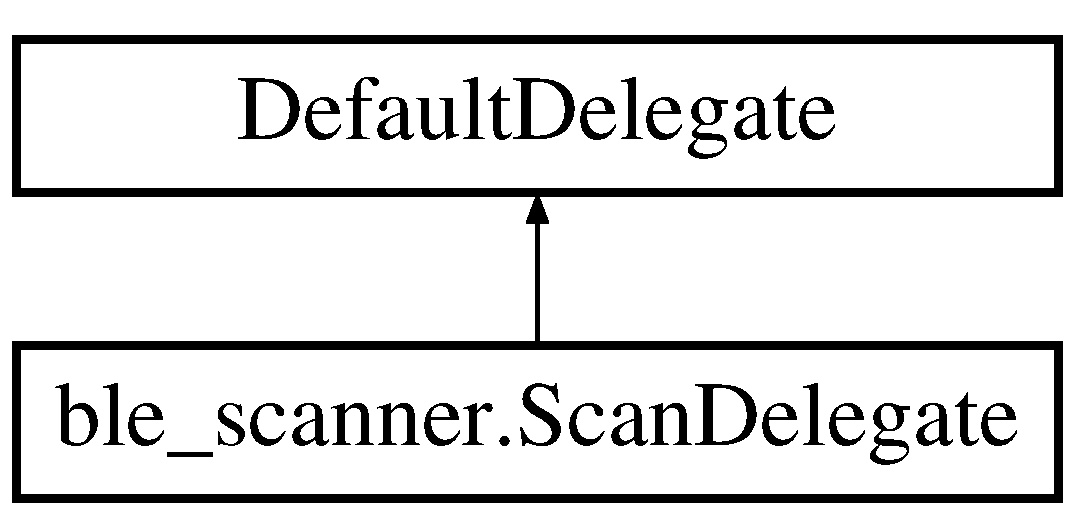
\includegraphics[height=2.000000cm]{classble__scanner_1_1ScanDelegate}
\end{center}
\end{figure}
\subsection*{Public Member Functions}
\begin{DoxyCompactItemize}
\item 
def \hyperlink{classble__scanner_1_1ScanDelegate_ac4160baa68bca5a0dd30405a4a71fca9}{\+\_\+\+\_\+init\+\_\+\+\_\+} (self)
\end{DoxyCompactItemize}


\subsection{Constructor \& Destructor Documentation}
\mbox{\Hypertarget{classble__scanner_1_1ScanDelegate_ac4160baa68bca5a0dd30405a4a71fca9}\label{classble__scanner_1_1ScanDelegate_ac4160baa68bca5a0dd30405a4a71fca9}} 
\index{ble\+\_\+scanner\+::\+Scan\+Delegate@{ble\+\_\+scanner\+::\+Scan\+Delegate}!\+\_\+\+\_\+init\+\_\+\+\_\+@{\+\_\+\+\_\+init\+\_\+\+\_\+}}
\index{\+\_\+\+\_\+init\+\_\+\+\_\+@{\+\_\+\+\_\+init\+\_\+\+\_\+}!ble\+\_\+scanner\+::\+Scan\+Delegate@{ble\+\_\+scanner\+::\+Scan\+Delegate}}
\subsubsection{\texorpdfstring{\+\_\+\+\_\+init\+\_\+\+\_\+()}{\_\_init\_\_()}}
{\footnotesize\ttfamily def ble\+\_\+scanner.\+Scan\+Delegate.\+\_\+\+\_\+init\+\_\+\+\_\+ (\begin{DoxyParamCaption}\item[{}]{self }\end{DoxyParamCaption})}



The documentation for this class was generated from the following file\+:\begin{DoxyCompactItemize}
\item 
src/\hyperlink{ble__scanner_8py}{ble\+\_\+scanner.\+py}\end{DoxyCompactItemize}

\hypertarget{classsensors_1_1sensors}{}\section{sensors.\+sensors Class Reference}
\label{classsensors_1_1sensors}\index{sensors.\+sensors@{sensors.\+sensors}}
Inheritance diagram for sensors.\+sensors\+:\begin{figure}[H]
\begin{center}
\leavevmode
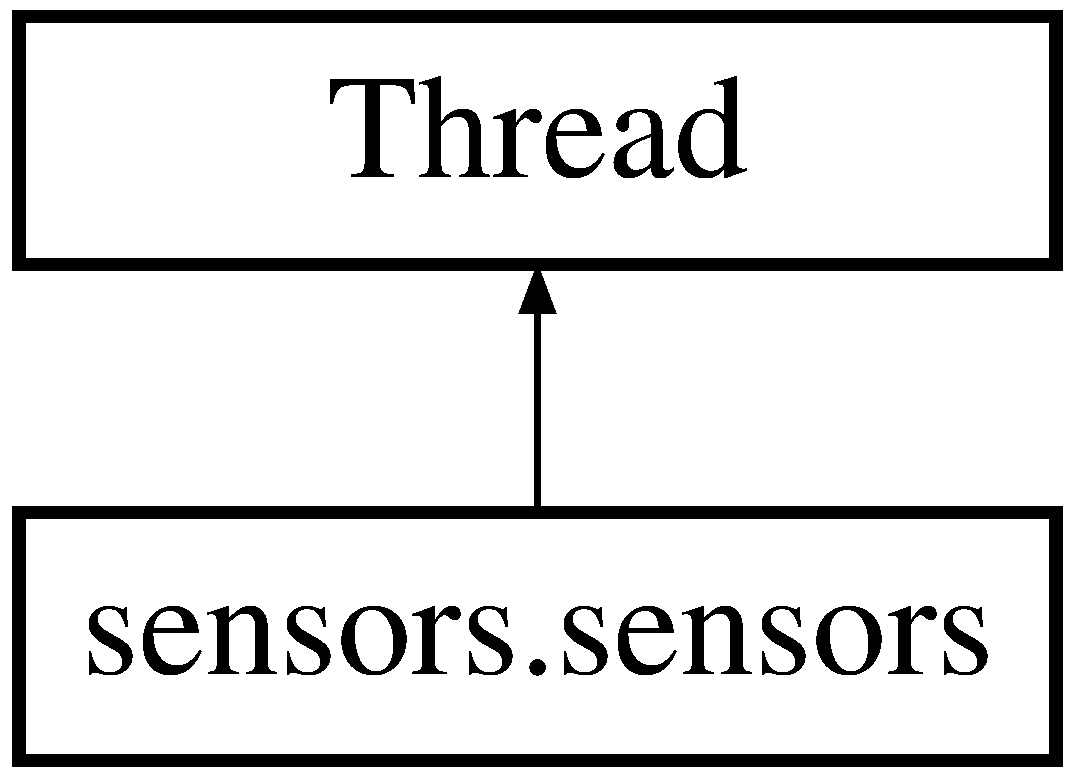
\includegraphics[height=2.000000cm]{classsensors_1_1sensors}
\end{center}
\end{figure}
\subsection*{Public Member Functions}
\begin{DoxyCompactItemize}
\item 
def \hyperlink{classsensors_1_1sensors_a88254be26dbf3f0c08e5619d2346c7ad}{\+\_\+\+\_\+init\+\_\+\+\_\+} (self, \hyperlink{classsensors_1_1sensors_a5bf11f0a0e2c85ca71f0c6b8315fe52e}{occ}, \hyperlink{classsensors_1_1sensors_a8eba6f72ffd7bafc1175d34212538646}{simulate}=False)
\item 
def \hyperlink{classsensors_1_1sensors_ac87befb2007bc2dc41183dd0f1bbf6fe}{init\+\_\+data\+\_\+from\+\_\+ride\+\_\+parameters} (self)
\item 
def \hyperlink{classsensors_1_1sensors_a5406a0c10ade1fca453cd70fb9e00ce3}{set\+\_\+ble\+\_\+device} (self, name, addr, dev\+\_\+type)
\item 
def \hyperlink{classsensors_1_1sensors_a7b076fab9aa6e370634f2c6833ee881a}{run} (self)
\item 
def \hyperlink{classsensors_1_1sensors_a8b62d241d6058127c7ffeea793ec4955}{set\+\_\+ble\+\_\+state} (self)
\item 
def \hyperlink{classsensors_1_1sensors_a5a7afd3c753b0e541a67f6c3f30eec2b}{get\+\_\+ble\+\_\+state} (self)
\item 
def \hyperlink{classsensors_1_1sensors_a36ff18450cb69c6b3bbcedf4aca05d0b}{get\+\_\+sensor} (self, name)
\item 
def \hyperlink{classsensors_1_1sensors_a7a53d09d9f55404f99601ac72e26e0ce}{reconnect\+\_\+sensor} (self, name)
\item 
def \hyperlink{classsensors_1_1sensors_a34571845bad702f6cb4a40100cb7df13}{\+\_\+\+\_\+del\+\_\+\+\_\+} (self)
\item 
def \hyperlink{classsensors_1_1sensors_afda843e462ec89881fbebcd6b636cc00}{stop} (self)
\end{DoxyCompactItemize}
\subsection*{Public Attributes}
\begin{DoxyCompactItemize}
\item 
\hyperlink{classsensors_1_1sensors_a27d75be18a7fce68b013503cf4519a51}{l}
\item 
\hyperlink{classsensors_1_1sensors_a5bf11f0a0e2c85ca71f0c6b8315fe52e}{occ}
\item 
\hyperlink{classsensors_1_1sensors_a847fa1597b64dec873fb946f51092237}{sensors}
\item 
\hyperlink{classsensors_1_1sensors_afbcf75bb28611a5e9b6a94ef6d5a68bf}{names}
\item 
\hyperlink{classsensors_1_1sensors_a20bd93d21715b480399592487cec59d0}{addrs}
\item 
\hyperlink{classsensors_1_1sensors_a8eba6f72ffd7bafc1175d34212538646}{simulate}
\item 
\hyperlink{classsensors_1_1sensors_af3c2abd825cd9c900148f9bf246df9d5}{ble\+\_\+state}
\item 
\hyperlink{classsensors_1_1sensors_aed7b543a8780e36b29ccc28197373730}{no\+\_\+of\+\_\+connected}
\item 
\hyperlink{classsensors_1_1sensors_abb353abbe46ec306c96974509aa1d235}{connecting}
\item 
\hyperlink{classsensors_1_1sensors_a182807b1ec751728080fda458ca8b294}{connected}
\item 
\hyperlink{classsensors_1_1sensors_a0fb70a27407e5cd15d34d63c4a5a2d39}{running}
\end{DoxyCompactItemize}


\subsection{Constructor \& Destructor Documentation}
\mbox{\Hypertarget{classsensors_1_1sensors_a88254be26dbf3f0c08e5619d2346c7ad}\label{classsensors_1_1sensors_a88254be26dbf3f0c08e5619d2346c7ad}} 
\index{sensors\+::sensors@{sensors\+::sensors}!\+\_\+\+\_\+init\+\_\+\+\_\+@{\+\_\+\+\_\+init\+\_\+\+\_\+}}
\index{\+\_\+\+\_\+init\+\_\+\+\_\+@{\+\_\+\+\_\+init\+\_\+\+\_\+}!sensors\+::sensors@{sensors\+::sensors}}
\subsubsection{\texorpdfstring{\+\_\+\+\_\+init\+\_\+\+\_\+()}{\_\_init\_\_()}}
{\footnotesize\ttfamily def sensors.\+sensors.\+\_\+\+\_\+init\+\_\+\+\_\+ (\begin{DoxyParamCaption}\item[{}]{self,  }\item[{}]{occ,  }\item[{}]{simulate = {\ttfamily False} }\end{DoxyParamCaption})}

\mbox{\Hypertarget{classsensors_1_1sensors_a34571845bad702f6cb4a40100cb7df13}\label{classsensors_1_1sensors_a34571845bad702f6cb4a40100cb7df13}} 
\index{sensors\+::sensors@{sensors\+::sensors}!\+\_\+\+\_\+del\+\_\+\+\_\+@{\+\_\+\+\_\+del\+\_\+\+\_\+}}
\index{\+\_\+\+\_\+del\+\_\+\+\_\+@{\+\_\+\+\_\+del\+\_\+\+\_\+}!sensors\+::sensors@{sensors\+::sensors}}
\subsubsection{\texorpdfstring{\+\_\+\+\_\+del\+\_\+\+\_\+()}{\_\_del\_\_()}}
{\footnotesize\ttfamily def sensors.\+sensors.\+\_\+\+\_\+del\+\_\+\+\_\+ (\begin{DoxyParamCaption}\item[{}]{self }\end{DoxyParamCaption})}



\subsection{Member Function Documentation}
\mbox{\Hypertarget{classsensors_1_1sensors_a5a7afd3c753b0e541a67f6c3f30eec2b}\label{classsensors_1_1sensors_a5a7afd3c753b0e541a67f6c3f30eec2b}} 
\index{sensors\+::sensors@{sensors\+::sensors}!get\+\_\+ble\+\_\+state@{get\+\_\+ble\+\_\+state}}
\index{get\+\_\+ble\+\_\+state@{get\+\_\+ble\+\_\+state}!sensors\+::sensors@{sensors\+::sensors}}
\subsubsection{\texorpdfstring{get\+\_\+ble\+\_\+state()}{get\_ble\_state()}}
{\footnotesize\ttfamily def sensors.\+sensors.\+get\+\_\+ble\+\_\+state (\begin{DoxyParamCaption}\item[{}]{self }\end{DoxyParamCaption})}

\mbox{\Hypertarget{classsensors_1_1sensors_a36ff18450cb69c6b3bbcedf4aca05d0b}\label{classsensors_1_1sensors_a36ff18450cb69c6b3bbcedf4aca05d0b}} 
\index{sensors\+::sensors@{sensors\+::sensors}!get\+\_\+sensor@{get\+\_\+sensor}}
\index{get\+\_\+sensor@{get\+\_\+sensor}!sensors\+::sensors@{sensors\+::sensors}}
\subsubsection{\texorpdfstring{get\+\_\+sensor()}{get\_sensor()}}
{\footnotesize\ttfamily def sensors.\+sensors.\+get\+\_\+sensor (\begin{DoxyParamCaption}\item[{}]{self,  }\item[{}]{name }\end{DoxyParamCaption})}

\mbox{\Hypertarget{classsensors_1_1sensors_ac87befb2007bc2dc41183dd0f1bbf6fe}\label{classsensors_1_1sensors_ac87befb2007bc2dc41183dd0f1bbf6fe}} 
\index{sensors\+::sensors@{sensors\+::sensors}!init\+\_\+data\+\_\+from\+\_\+ride\+\_\+parameters@{init\+\_\+data\+\_\+from\+\_\+ride\+\_\+parameters}}
\index{init\+\_\+data\+\_\+from\+\_\+ride\+\_\+parameters@{init\+\_\+data\+\_\+from\+\_\+ride\+\_\+parameters}!sensors\+::sensors@{sensors\+::sensors}}
\subsubsection{\texorpdfstring{init\+\_\+data\+\_\+from\+\_\+ride\+\_\+parameters()}{init\_data\_from\_ride\_parameters()}}
{\footnotesize\ttfamily def sensors.\+sensors.\+init\+\_\+data\+\_\+from\+\_\+ride\+\_\+parameters (\begin{DoxyParamCaption}\item[{}]{self }\end{DoxyParamCaption})}

\mbox{\Hypertarget{classsensors_1_1sensors_a7a53d09d9f55404f99601ac72e26e0ce}\label{classsensors_1_1sensors_a7a53d09d9f55404f99601ac72e26e0ce}} 
\index{sensors\+::sensors@{sensors\+::sensors}!reconnect\+\_\+sensor@{reconnect\+\_\+sensor}}
\index{reconnect\+\_\+sensor@{reconnect\+\_\+sensor}!sensors\+::sensors@{sensors\+::sensors}}
\subsubsection{\texorpdfstring{reconnect\+\_\+sensor()}{reconnect\_sensor()}}
{\footnotesize\ttfamily def sensors.\+sensors.\+reconnect\+\_\+sensor (\begin{DoxyParamCaption}\item[{}]{self,  }\item[{}]{name }\end{DoxyParamCaption})}

\mbox{\Hypertarget{classsensors_1_1sensors_a7b076fab9aa6e370634f2c6833ee881a}\label{classsensors_1_1sensors_a7b076fab9aa6e370634f2c6833ee881a}} 
\index{sensors\+::sensors@{sensors\+::sensors}!run@{run}}
\index{run@{run}!sensors\+::sensors@{sensors\+::sensors}}
\subsubsection{\texorpdfstring{run()}{run()}}
{\footnotesize\ttfamily def sensors.\+sensors.\+run (\begin{DoxyParamCaption}\item[{}]{self }\end{DoxyParamCaption})}

\mbox{\Hypertarget{classsensors_1_1sensors_a5406a0c10ade1fca453cd70fb9e00ce3}\label{classsensors_1_1sensors_a5406a0c10ade1fca453cd70fb9e00ce3}} 
\index{sensors\+::sensors@{sensors\+::sensors}!set\+\_\+ble\+\_\+device@{set\+\_\+ble\+\_\+device}}
\index{set\+\_\+ble\+\_\+device@{set\+\_\+ble\+\_\+device}!sensors\+::sensors@{sensors\+::sensors}}
\subsubsection{\texorpdfstring{set\+\_\+ble\+\_\+device()}{set\_ble\_device()}}
{\footnotesize\ttfamily def sensors.\+sensors.\+set\+\_\+ble\+\_\+device (\begin{DoxyParamCaption}\item[{}]{self,  }\item[{}]{name,  }\item[{}]{addr,  }\item[{}]{dev\+\_\+type }\end{DoxyParamCaption})}

\mbox{\Hypertarget{classsensors_1_1sensors_a8b62d241d6058127c7ffeea793ec4955}\label{classsensors_1_1sensors_a8b62d241d6058127c7ffeea793ec4955}} 
\index{sensors\+::sensors@{sensors\+::sensors}!set\+\_\+ble\+\_\+state@{set\+\_\+ble\+\_\+state}}
\index{set\+\_\+ble\+\_\+state@{set\+\_\+ble\+\_\+state}!sensors\+::sensors@{sensors\+::sensors}}
\subsubsection{\texorpdfstring{set\+\_\+ble\+\_\+state()}{set\_ble\_state()}}
{\footnotesize\ttfamily def sensors.\+sensors.\+set\+\_\+ble\+\_\+state (\begin{DoxyParamCaption}\item[{}]{self }\end{DoxyParamCaption})}

\mbox{\Hypertarget{classsensors_1_1sensors_afda843e462ec89881fbebcd6b636cc00}\label{classsensors_1_1sensors_afda843e462ec89881fbebcd6b636cc00}} 
\index{sensors\+::sensors@{sensors\+::sensors}!stop@{stop}}
\index{stop@{stop}!sensors\+::sensors@{sensors\+::sensors}}
\subsubsection{\texorpdfstring{stop()}{stop()}}
{\footnotesize\ttfamily def sensors.\+sensors.\+stop (\begin{DoxyParamCaption}\item[{}]{self }\end{DoxyParamCaption})}



\subsection{Member Data Documentation}
\mbox{\Hypertarget{classsensors_1_1sensors_a20bd93d21715b480399592487cec59d0}\label{classsensors_1_1sensors_a20bd93d21715b480399592487cec59d0}} 
\index{sensors\+::sensors@{sensors\+::sensors}!addrs@{addrs}}
\index{addrs@{addrs}!sensors\+::sensors@{sensors\+::sensors}}
\subsubsection{\texorpdfstring{addrs}{addrs}}
{\footnotesize\ttfamily sensors.\+sensors.\+addrs}

\mbox{\Hypertarget{classsensors_1_1sensors_af3c2abd825cd9c900148f9bf246df9d5}\label{classsensors_1_1sensors_af3c2abd825cd9c900148f9bf246df9d5}} 
\index{sensors\+::sensors@{sensors\+::sensors}!ble\+\_\+state@{ble\+\_\+state}}
\index{ble\+\_\+state@{ble\+\_\+state}!sensors\+::sensors@{sensors\+::sensors}}
\subsubsection{\texorpdfstring{ble\+\_\+state}{ble\_state}}
{\footnotesize\ttfamily sensors.\+sensors.\+ble\+\_\+state}

\mbox{\Hypertarget{classsensors_1_1sensors_a182807b1ec751728080fda458ca8b294}\label{classsensors_1_1sensors_a182807b1ec751728080fda458ca8b294}} 
\index{sensors\+::sensors@{sensors\+::sensors}!connected@{connected}}
\index{connected@{connected}!sensors\+::sensors@{sensors\+::sensors}}
\subsubsection{\texorpdfstring{connected}{connected}}
{\footnotesize\ttfamily sensors.\+sensors.\+connected}

\mbox{\Hypertarget{classsensors_1_1sensors_abb353abbe46ec306c96974509aa1d235}\label{classsensors_1_1sensors_abb353abbe46ec306c96974509aa1d235}} 
\index{sensors\+::sensors@{sensors\+::sensors}!connecting@{connecting}}
\index{connecting@{connecting}!sensors\+::sensors@{sensors\+::sensors}}
\subsubsection{\texorpdfstring{connecting}{connecting}}
{\footnotesize\ttfamily sensors.\+sensors.\+connecting}

\mbox{\Hypertarget{classsensors_1_1sensors_a27d75be18a7fce68b013503cf4519a51}\label{classsensors_1_1sensors_a27d75be18a7fce68b013503cf4519a51}} 
\index{sensors\+::sensors@{sensors\+::sensors}!l@{l}}
\index{l@{l}!sensors\+::sensors@{sensors\+::sensors}}
\subsubsection{\texorpdfstring{l}{l}}
{\footnotesize\ttfamily sensors.\+sensors.\+l}

\mbox{\Hypertarget{classsensors_1_1sensors_afbcf75bb28611a5e9b6a94ef6d5a68bf}\label{classsensors_1_1sensors_afbcf75bb28611a5e9b6a94ef6d5a68bf}} 
\index{sensors\+::sensors@{sensors\+::sensors}!names@{names}}
\index{names@{names}!sensors\+::sensors@{sensors\+::sensors}}
\subsubsection{\texorpdfstring{names}{names}}
{\footnotesize\ttfamily sensors.\+sensors.\+names}

\mbox{\Hypertarget{classsensors_1_1sensors_aed7b543a8780e36b29ccc28197373730}\label{classsensors_1_1sensors_aed7b543a8780e36b29ccc28197373730}} 
\index{sensors\+::sensors@{sensors\+::sensors}!no\+\_\+of\+\_\+connected@{no\+\_\+of\+\_\+connected}}
\index{no\+\_\+of\+\_\+connected@{no\+\_\+of\+\_\+connected}!sensors\+::sensors@{sensors\+::sensors}}
\subsubsection{\texorpdfstring{no\+\_\+of\+\_\+connected}{no\_of\_connected}}
{\footnotesize\ttfamily sensors.\+sensors.\+no\+\_\+of\+\_\+connected}

\mbox{\Hypertarget{classsensors_1_1sensors_a5bf11f0a0e2c85ca71f0c6b8315fe52e}\label{classsensors_1_1sensors_a5bf11f0a0e2c85ca71f0c6b8315fe52e}} 
\index{sensors\+::sensors@{sensors\+::sensors}!occ@{occ}}
\index{occ@{occ}!sensors\+::sensors@{sensors\+::sensors}}
\subsubsection{\texorpdfstring{occ}{occ}}
{\footnotesize\ttfamily sensors.\+sensors.\+occ}

\mbox{\Hypertarget{classsensors_1_1sensors_a0fb70a27407e5cd15d34d63c4a5a2d39}\label{classsensors_1_1sensors_a0fb70a27407e5cd15d34d63c4a5a2d39}} 
\index{sensors\+::sensors@{sensors\+::sensors}!running@{running}}
\index{running@{running}!sensors\+::sensors@{sensors\+::sensors}}
\subsubsection{\texorpdfstring{running}{running}}
{\footnotesize\ttfamily sensors.\+sensors.\+running}

\mbox{\Hypertarget{classsensors_1_1sensors_a847fa1597b64dec873fb946f51092237}\label{classsensors_1_1sensors_a847fa1597b64dec873fb946f51092237}} 
\index{sensors\+::sensors@{sensors\+::sensors}!sensors@{sensors}}
\index{sensors@{sensors}!sensors\+::sensors@{sensors\+::sensors}}
\subsubsection{\texorpdfstring{sensors}{sensors}}
{\footnotesize\ttfamily sensors.\+sensors.\+sensors}

\mbox{\Hypertarget{classsensors_1_1sensors_a8eba6f72ffd7bafc1175d34212538646}\label{classsensors_1_1sensors_a8eba6f72ffd7bafc1175d34212538646}} 
\index{sensors\+::sensors@{sensors\+::sensors}!simulate@{simulate}}
\index{simulate@{simulate}!sensors\+::sensors@{sensors\+::sensors}}
\subsubsection{\texorpdfstring{simulate}{simulate}}
{\footnotesize\ttfamily sensors.\+sensors.\+simulate}



The documentation for this class was generated from the following file\+:\begin{DoxyCompactItemize}
\item 
src/\hyperlink{sensors_8py}{sensors.\+py}\end{DoxyCompactItemize}

\hypertarget{classunits_1_1units}{}\section{units.\+units Class Reference}
\label{classunits_1_1units}\index{units.\+units@{units.\+units}}
\subsection*{Public Member Functions}
\begin{DoxyCompactItemize}
\item 
def \hyperlink{classunits_1_1units_a5127edbff09fdefbbd817b8fe069e3c9}{\+\_\+\+\_\+init\+\_\+\+\_\+} (self)
\item 
def \hyperlink{classunits_1_1units_a9c3f8fdf21305ae05a38649233549925}{convert} (self, value, target\+\_\+unit)
\item 
def \hyperlink{classunits_1_1units_a59cb803b7f3f34fec224e047ded48cdb}{temp\+\_\+\+C\+\_\+to\+\_\+F} (self, temp)
\item 
def \hyperlink{classunits_1_1units_aacbd2271524a124c433305cab790b496}{temp\+\_\+\+C\+\_\+to\+\_\+K} (self, temp)
\item 
def \hyperlink{classunits_1_1units_a36d19243c733324f4d3779ab047f6775}{speed\+\_\+ms\+\_\+to\+\_\+kmh} (self, \hyperlink{namespaceunits_a759e0d0478b90aaac881c06441083170}{speed})
\item 
def \hyperlink{classunits_1_1units_a9ca0a3b531dd6d580a5f50d47250a889}{speed\+\_\+ms\+\_\+to\+\_\+mph} (self, \hyperlink{namespaceunits_a759e0d0478b90aaac881c06441083170}{speed})
\item 
def \hyperlink{classunits_1_1units_a0c0d36f959513967d3e67d91741f382e}{mass\+\_\+kg\+\_\+to\+\_\+pd} (self, \hyperlink{namespaceunits_a56758bcc2c4dd39571c297387d4a5a20}{mass})
\item 
def \hyperlink{classunits_1_1units_acb3efb0b7dc98e5f816417cd520817fd}{mass\+\_\+kg\+\_\+to\+\_\+st} (self, \hyperlink{namespaceunits_a56758bcc2c4dd39571c297387d4a5a20}{mass})
\item 
def \hyperlink{classunits_1_1units_a175b076c9d2796e620b66646b1a85eac}{mass\+\_\+kg\+\_\+to\+\_\+lb} (self, \hyperlink{namespaceunits_a56758bcc2c4dd39571c297387d4a5a20}{mass})
\item 
def \hyperlink{classunits_1_1units_a530de99e13adbee5b18256aa060cf032}{dist\+\_\+m\+\_\+to\+\_\+km} (self, \hyperlink{namespaceunits_ab66c7acd86085e0dd596e5835d5f020a}{dist})
\item 
def \hyperlink{classunits_1_1units_aa70deff236b3144c9346462e7db4c435}{dist\+\_\+m\+\_\+to\+\_\+mi} (self, \hyperlink{namespaceunits_ab66c7acd86085e0dd596e5835d5f020a}{dist})
\item 
def \hyperlink{classunits_1_1units_a9b2dea593e393a0a66420f4e4596ac1b}{dist\+\_\+m\+\_\+to\+\_\+yd} (self, \hyperlink{namespaceunits_ab66c7acd86085e0dd596e5835d5f020a}{dist})
\item 
def \hyperlink{classunits_1_1units_a981725c0877d96a44b774cc44e9a5cb0}{m\+\_\+m\+\_\+to\+\_\+percent} (self, value)
\item 
def \hyperlink{classunits_1_1units_a2f4c5ca2d50b1df9bb0526a908b351dc}{pressure\+\_\+\+Pa\+\_\+to\+\_\+h\+Pa} (self, value)
\end{DoxyCompactItemize}


\subsection{Constructor \& Destructor Documentation}
\mbox{\Hypertarget{classunits_1_1units_a5127edbff09fdefbbd817b8fe069e3c9}\label{classunits_1_1units_a5127edbff09fdefbbd817b8fe069e3c9}} 
\index{units\+::units@{units\+::units}!\+\_\+\+\_\+init\+\_\+\+\_\+@{\+\_\+\+\_\+init\+\_\+\+\_\+}}
\index{\+\_\+\+\_\+init\+\_\+\+\_\+@{\+\_\+\+\_\+init\+\_\+\+\_\+}!units\+::units@{units\+::units}}
\subsubsection{\texorpdfstring{\+\_\+\+\_\+init\+\_\+\+\_\+()}{\_\_init\_\_()}}
{\footnotesize\ttfamily def units.\+units.\+\_\+\+\_\+init\+\_\+\+\_\+ (\begin{DoxyParamCaption}\item[{}]{self }\end{DoxyParamCaption})}



\subsection{Member Function Documentation}
\mbox{\Hypertarget{classunits_1_1units_a9c3f8fdf21305ae05a38649233549925}\label{classunits_1_1units_a9c3f8fdf21305ae05a38649233549925}} 
\index{units\+::units@{units\+::units}!convert@{convert}}
\index{convert@{convert}!units\+::units@{units\+::units}}
\subsubsection{\texorpdfstring{convert()}{convert()}}
{\footnotesize\ttfamily def units.\+units.\+convert (\begin{DoxyParamCaption}\item[{}]{self,  }\item[{}]{value,  }\item[{}]{target\+\_\+unit }\end{DoxyParamCaption})}

\mbox{\Hypertarget{classunits_1_1units_a530de99e13adbee5b18256aa060cf032}\label{classunits_1_1units_a530de99e13adbee5b18256aa060cf032}} 
\index{units\+::units@{units\+::units}!dist\+\_\+m\+\_\+to\+\_\+km@{dist\+\_\+m\+\_\+to\+\_\+km}}
\index{dist\+\_\+m\+\_\+to\+\_\+km@{dist\+\_\+m\+\_\+to\+\_\+km}!units\+::units@{units\+::units}}
\subsubsection{\texorpdfstring{dist\+\_\+m\+\_\+to\+\_\+km()}{dist\_m\_to\_km()}}
{\footnotesize\ttfamily def units.\+units.\+dist\+\_\+m\+\_\+to\+\_\+km (\begin{DoxyParamCaption}\item[{}]{self,  }\item[{}]{dist }\end{DoxyParamCaption})}

\mbox{\Hypertarget{classunits_1_1units_aa70deff236b3144c9346462e7db4c435}\label{classunits_1_1units_aa70deff236b3144c9346462e7db4c435}} 
\index{units\+::units@{units\+::units}!dist\+\_\+m\+\_\+to\+\_\+mi@{dist\+\_\+m\+\_\+to\+\_\+mi}}
\index{dist\+\_\+m\+\_\+to\+\_\+mi@{dist\+\_\+m\+\_\+to\+\_\+mi}!units\+::units@{units\+::units}}
\subsubsection{\texorpdfstring{dist\+\_\+m\+\_\+to\+\_\+mi()}{dist\_m\_to\_mi()}}
{\footnotesize\ttfamily def units.\+units.\+dist\+\_\+m\+\_\+to\+\_\+mi (\begin{DoxyParamCaption}\item[{}]{self,  }\item[{}]{dist }\end{DoxyParamCaption})}

\mbox{\Hypertarget{classunits_1_1units_a9b2dea593e393a0a66420f4e4596ac1b}\label{classunits_1_1units_a9b2dea593e393a0a66420f4e4596ac1b}} 
\index{units\+::units@{units\+::units}!dist\+\_\+m\+\_\+to\+\_\+yd@{dist\+\_\+m\+\_\+to\+\_\+yd}}
\index{dist\+\_\+m\+\_\+to\+\_\+yd@{dist\+\_\+m\+\_\+to\+\_\+yd}!units\+::units@{units\+::units}}
\subsubsection{\texorpdfstring{dist\+\_\+m\+\_\+to\+\_\+yd()}{dist\_m\_to\_yd()}}
{\footnotesize\ttfamily def units.\+units.\+dist\+\_\+m\+\_\+to\+\_\+yd (\begin{DoxyParamCaption}\item[{}]{self,  }\item[{}]{dist }\end{DoxyParamCaption})}

\mbox{\Hypertarget{classunits_1_1units_a981725c0877d96a44b774cc44e9a5cb0}\label{classunits_1_1units_a981725c0877d96a44b774cc44e9a5cb0}} 
\index{units\+::units@{units\+::units}!m\+\_\+m\+\_\+to\+\_\+percent@{m\+\_\+m\+\_\+to\+\_\+percent}}
\index{m\+\_\+m\+\_\+to\+\_\+percent@{m\+\_\+m\+\_\+to\+\_\+percent}!units\+::units@{units\+::units}}
\subsubsection{\texorpdfstring{m\+\_\+m\+\_\+to\+\_\+percent()}{m\_m\_to\_percent()}}
{\footnotesize\ttfamily def units.\+units.\+m\+\_\+m\+\_\+to\+\_\+percent (\begin{DoxyParamCaption}\item[{}]{self,  }\item[{}]{value }\end{DoxyParamCaption})}

\mbox{\Hypertarget{classunits_1_1units_a175b076c9d2796e620b66646b1a85eac}\label{classunits_1_1units_a175b076c9d2796e620b66646b1a85eac}} 
\index{units\+::units@{units\+::units}!mass\+\_\+kg\+\_\+to\+\_\+lb@{mass\+\_\+kg\+\_\+to\+\_\+lb}}
\index{mass\+\_\+kg\+\_\+to\+\_\+lb@{mass\+\_\+kg\+\_\+to\+\_\+lb}!units\+::units@{units\+::units}}
\subsubsection{\texorpdfstring{mass\+\_\+kg\+\_\+to\+\_\+lb()}{mass\_kg\_to\_lb()}}
{\footnotesize\ttfamily def units.\+units.\+mass\+\_\+kg\+\_\+to\+\_\+lb (\begin{DoxyParamCaption}\item[{}]{self,  }\item[{}]{mass }\end{DoxyParamCaption})}

\mbox{\Hypertarget{classunits_1_1units_a0c0d36f959513967d3e67d91741f382e}\label{classunits_1_1units_a0c0d36f959513967d3e67d91741f382e}} 
\index{units\+::units@{units\+::units}!mass\+\_\+kg\+\_\+to\+\_\+pd@{mass\+\_\+kg\+\_\+to\+\_\+pd}}
\index{mass\+\_\+kg\+\_\+to\+\_\+pd@{mass\+\_\+kg\+\_\+to\+\_\+pd}!units\+::units@{units\+::units}}
\subsubsection{\texorpdfstring{mass\+\_\+kg\+\_\+to\+\_\+pd()}{mass\_kg\_to\_pd()}}
{\footnotesize\ttfamily def units.\+units.\+mass\+\_\+kg\+\_\+to\+\_\+pd (\begin{DoxyParamCaption}\item[{}]{self,  }\item[{}]{mass }\end{DoxyParamCaption})}

\mbox{\Hypertarget{classunits_1_1units_acb3efb0b7dc98e5f816417cd520817fd}\label{classunits_1_1units_acb3efb0b7dc98e5f816417cd520817fd}} 
\index{units\+::units@{units\+::units}!mass\+\_\+kg\+\_\+to\+\_\+st@{mass\+\_\+kg\+\_\+to\+\_\+st}}
\index{mass\+\_\+kg\+\_\+to\+\_\+st@{mass\+\_\+kg\+\_\+to\+\_\+st}!units\+::units@{units\+::units}}
\subsubsection{\texorpdfstring{mass\+\_\+kg\+\_\+to\+\_\+st()}{mass\_kg\_to\_st()}}
{\footnotesize\ttfamily def units.\+units.\+mass\+\_\+kg\+\_\+to\+\_\+st (\begin{DoxyParamCaption}\item[{}]{self,  }\item[{}]{mass }\end{DoxyParamCaption})}

\mbox{\Hypertarget{classunits_1_1units_a2f4c5ca2d50b1df9bb0526a908b351dc}\label{classunits_1_1units_a2f4c5ca2d50b1df9bb0526a908b351dc}} 
\index{units\+::units@{units\+::units}!pressure\+\_\+\+Pa\+\_\+to\+\_\+h\+Pa@{pressure\+\_\+\+Pa\+\_\+to\+\_\+h\+Pa}}
\index{pressure\+\_\+\+Pa\+\_\+to\+\_\+h\+Pa@{pressure\+\_\+\+Pa\+\_\+to\+\_\+h\+Pa}!units\+::units@{units\+::units}}
\subsubsection{\texorpdfstring{pressure\+\_\+\+Pa\+\_\+to\+\_\+h\+Pa()}{pressure\_Pa\_to\_hPa()}}
{\footnotesize\ttfamily def units.\+units.\+pressure\+\_\+\+Pa\+\_\+to\+\_\+h\+Pa (\begin{DoxyParamCaption}\item[{}]{self,  }\item[{}]{value }\end{DoxyParamCaption})}

\mbox{\Hypertarget{classunits_1_1units_a36d19243c733324f4d3779ab047f6775}\label{classunits_1_1units_a36d19243c733324f4d3779ab047f6775}} 
\index{units\+::units@{units\+::units}!speed\+\_\+ms\+\_\+to\+\_\+kmh@{speed\+\_\+ms\+\_\+to\+\_\+kmh}}
\index{speed\+\_\+ms\+\_\+to\+\_\+kmh@{speed\+\_\+ms\+\_\+to\+\_\+kmh}!units\+::units@{units\+::units}}
\subsubsection{\texorpdfstring{speed\+\_\+ms\+\_\+to\+\_\+kmh()}{speed\_ms\_to\_kmh()}}
{\footnotesize\ttfamily def units.\+units.\+speed\+\_\+ms\+\_\+to\+\_\+kmh (\begin{DoxyParamCaption}\item[{}]{self,  }\item[{}]{speed }\end{DoxyParamCaption})}

\mbox{\Hypertarget{classunits_1_1units_a9ca0a3b531dd6d580a5f50d47250a889}\label{classunits_1_1units_a9ca0a3b531dd6d580a5f50d47250a889}} 
\index{units\+::units@{units\+::units}!speed\+\_\+ms\+\_\+to\+\_\+mph@{speed\+\_\+ms\+\_\+to\+\_\+mph}}
\index{speed\+\_\+ms\+\_\+to\+\_\+mph@{speed\+\_\+ms\+\_\+to\+\_\+mph}!units\+::units@{units\+::units}}
\subsubsection{\texorpdfstring{speed\+\_\+ms\+\_\+to\+\_\+mph()}{speed\_ms\_to\_mph()}}
{\footnotesize\ttfamily def units.\+units.\+speed\+\_\+ms\+\_\+to\+\_\+mph (\begin{DoxyParamCaption}\item[{}]{self,  }\item[{}]{speed }\end{DoxyParamCaption})}

\mbox{\Hypertarget{classunits_1_1units_a59cb803b7f3f34fec224e047ded48cdb}\label{classunits_1_1units_a59cb803b7f3f34fec224e047ded48cdb}} 
\index{units\+::units@{units\+::units}!temp\+\_\+\+C\+\_\+to\+\_\+F@{temp\+\_\+\+C\+\_\+to\+\_\+F}}
\index{temp\+\_\+\+C\+\_\+to\+\_\+F@{temp\+\_\+\+C\+\_\+to\+\_\+F}!units\+::units@{units\+::units}}
\subsubsection{\texorpdfstring{temp\+\_\+\+C\+\_\+to\+\_\+\+F()}{temp\_C\_to\_F()}}
{\footnotesize\ttfamily def units.\+units.\+temp\+\_\+\+C\+\_\+to\+\_\+F (\begin{DoxyParamCaption}\item[{}]{self,  }\item[{}]{temp }\end{DoxyParamCaption})}

\mbox{\Hypertarget{classunits_1_1units_aacbd2271524a124c433305cab790b496}\label{classunits_1_1units_aacbd2271524a124c433305cab790b496}} 
\index{units\+::units@{units\+::units}!temp\+\_\+\+C\+\_\+to\+\_\+K@{temp\+\_\+\+C\+\_\+to\+\_\+K}}
\index{temp\+\_\+\+C\+\_\+to\+\_\+K@{temp\+\_\+\+C\+\_\+to\+\_\+K}!units\+::units@{units\+::units}}
\subsubsection{\texorpdfstring{temp\+\_\+\+C\+\_\+to\+\_\+\+K()}{temp\_C\_to\_K()}}
{\footnotesize\ttfamily def units.\+units.\+temp\+\_\+\+C\+\_\+to\+\_\+K (\begin{DoxyParamCaption}\item[{}]{self,  }\item[{}]{temp }\end{DoxyParamCaption})}



The documentation for this class was generated from the following file\+:\begin{DoxyCompactItemize}
\item 
src/\hyperlink{units_8py}{units.\+py}\end{DoxyCompactItemize}

\hypertarget{classwheel_1_1wheel}{}\section{wheel.\+wheel Class Reference}
\label{classwheel_1_1wheel}\index{wheel.\+wheel@{wheel.\+wheel}}
\subsection*{Public Member Functions}
\begin{DoxyCompactItemize}
\item 
def \hyperlink{classwheel_1_1wheel_ad74f17bf918fd53ed5e62566ee367dab}{\+\_\+\+\_\+init\+\_\+\+\_\+} (self)
\item 
def \hyperlink{classwheel_1_1wheel_a2c8cb4fefde6714812f8d362b8744a63}{get\+\_\+size} (self, name)
\end{DoxyCompactItemize}
\subsection*{Public Attributes}
\begin{DoxyCompactItemize}
\item 
\hyperlink{classwheel_1_1wheel_ad2bdaadaaf22bc7522c6c579e9c2d6d8}{wheel\+\_\+size}
\end{DoxyCompactItemize}


\subsection{Constructor \& Destructor Documentation}
\mbox{\Hypertarget{classwheel_1_1wheel_ad74f17bf918fd53ed5e62566ee367dab}\label{classwheel_1_1wheel_ad74f17bf918fd53ed5e62566ee367dab}} 
\index{wheel\+::wheel@{wheel\+::wheel}!\+\_\+\+\_\+init\+\_\+\+\_\+@{\+\_\+\+\_\+init\+\_\+\+\_\+}}
\index{\+\_\+\+\_\+init\+\_\+\+\_\+@{\+\_\+\+\_\+init\+\_\+\+\_\+}!wheel\+::wheel@{wheel\+::wheel}}
\subsubsection{\texorpdfstring{\+\_\+\+\_\+init\+\_\+\+\_\+()}{\_\_init\_\_()}}
{\footnotesize\ttfamily def wheel.\+wheel.\+\_\+\+\_\+init\+\_\+\+\_\+ (\begin{DoxyParamCaption}\item[{}]{self }\end{DoxyParamCaption})}



\subsection{Member Function Documentation}
\mbox{\Hypertarget{classwheel_1_1wheel_a2c8cb4fefde6714812f8d362b8744a63}\label{classwheel_1_1wheel_a2c8cb4fefde6714812f8d362b8744a63}} 
\index{wheel\+::wheel@{wheel\+::wheel}!get\+\_\+size@{get\+\_\+size}}
\index{get\+\_\+size@{get\+\_\+size}!wheel\+::wheel@{wheel\+::wheel}}
\subsubsection{\texorpdfstring{get\+\_\+size()}{get\_size()}}
{\footnotesize\ttfamily def wheel.\+wheel.\+get\+\_\+size (\begin{DoxyParamCaption}\item[{}]{self,  }\item[{}]{name }\end{DoxyParamCaption})}



\subsection{Member Data Documentation}
\mbox{\Hypertarget{classwheel_1_1wheel_ad2bdaadaaf22bc7522c6c579e9c2d6d8}\label{classwheel_1_1wheel_ad2bdaadaaf22bc7522c6c579e9c2d6d8}} 
\index{wheel\+::wheel@{wheel\+::wheel}!wheel\+\_\+size@{wheel\+\_\+size}}
\index{wheel\+\_\+size@{wheel\+\_\+size}!wheel\+::wheel@{wheel\+::wheel}}
\subsubsection{\texorpdfstring{wheel\+\_\+size}{wheel\_size}}
{\footnotesize\ttfamily wheel.\+wheel.\+wheel\+\_\+size}



The documentation for this class was generated from the following file\+:\begin{DoxyCompactItemize}
\item 
src/\hyperlink{wheel_8py}{wheel.\+py}\end{DoxyCompactItemize}

\chapter{File Documentation}
\hypertarget{ble__hr_8py}{}\section{src/ble\+\_\+hr.py File Reference}
\label{ble__hr_8py}\index{src/ble\+\_\+hr.\+py@{src/ble\+\_\+hr.\+py}}
\subsection*{Classes}
\begin{DoxyCompactItemize}
\item 
class \hyperlink{classble__hr_1_1ble__hr}{ble\+\_\+hr.\+ble\+\_\+hr}
\item 
class \hyperlink{classble__hr_1_1HR__Delegate}{ble\+\_\+hr.\+H\+R\+\_\+\+Delegate}
\end{DoxyCompactItemize}
\subsection*{Namespaces}
\begin{DoxyCompactItemize}
\item 
 \hyperlink{namespaceble__hr}{ble\+\_\+hr}
\end{DoxyCompactItemize}

\hypertarget{ble__sc_8py}{}\section{src/ble\+\_\+sc.py File Reference}
\label{ble__sc_8py}\index{src/ble\+\_\+sc.\+py@{src/ble\+\_\+sc.\+py}}
\subsection*{Classes}
\begin{DoxyCompactItemize}
\item 
class \hyperlink{classble__sc_1_1ble__sc}{ble\+\_\+sc.\+ble\+\_\+sc}
\item 
class \hyperlink{classble__sc_1_1CSC__Delegate}{ble\+\_\+sc.\+C\+S\+C\+\_\+\+Delegate}
\end{DoxyCompactItemize}
\subsection*{Namespaces}
\begin{DoxyCompactItemize}
\item 
 \hyperlink{namespaceble__sc}{ble\+\_\+sc}
\end{DoxyCompactItemize}

\hypertarget{ble__scanner_8py}{}\section{src/ble\+\_\+scanner.py File Reference}
\label{ble__scanner_8py}\index{src/ble\+\_\+scanner.\+py@{src/ble\+\_\+scanner.\+py}}
\subsection*{Classes}
\begin{DoxyCompactItemize}
\item 
class \hyperlink{classble__scanner_1_1ScanDelegate}{ble\+\_\+scanner.\+Scan\+Delegate}
\item 
class \hyperlink{classble__scanner_1_1ble__scan}{ble\+\_\+scanner.\+ble\+\_\+scan}
\end{DoxyCompactItemize}
\subsection*{Namespaces}
\begin{DoxyCompactItemize}
\item 
 \hyperlink{namespaceble__scanner}{ble\+\_\+scanner}
\end{DoxyCompactItemize}
\subsection*{Variables}
\begin{DoxyCompactItemize}
\item 
\hyperlink{namespaceble__scanner_a7a11ffc3e3fa4e63a3699a3c0a35fea0}{ble\+\_\+scanner.\+ble} = ble\+\_\+scan()
\end{DoxyCompactItemize}

\hypertarget{bmp183_8py}{}\section{src/bmp183.py File Reference}
\label{bmp183_8py}\index{src/bmp183.\+py@{src/bmp183.\+py}}
\subsection*{Classes}
\begin{DoxyCompactItemize}
\item 
class \hyperlink{classbmp183_1_1bmp183}{bmp183.\+bmp183}
\end{DoxyCompactItemize}
\subsection*{Namespaces}
\begin{DoxyCompactItemize}
\item 
 \hyperlink{namespacebmp183}{bmp183}
\end{DoxyCompactItemize}
\subsection*{Variables}
\begin{DoxyCompactItemize}
\item 
\hyperlink{namespacebmp183_a2c3926dd39f72e83d5c9203297c7a998}{bmp183.\+NaN} = float(\textquotesingle{}nan\textquotesingle{})
\end{DoxyCompactItemize}

\hypertarget{config_8py}{}\section{src/config.py File Reference}
\label{config_8py}\index{src/config.\+py@{src/config.\+py}}
\subsection*{Classes}
\begin{DoxyCompactItemize}
\item 
class \hyperlink{classconfig_1_1config}{config.\+config}
\end{DoxyCompactItemize}
\subsection*{Namespaces}
\begin{DoxyCompactItemize}
\item 
 \hyperlink{namespaceconfig}{config}
\end{DoxyCompactItemize}

\hypertarget{gps__mtk3339_8py}{}\section{src/gps\+\_\+mtk3339.py File Reference}
\label{gps__mtk3339_8py}\index{src/gps\+\_\+mtk3339.\+py@{src/gps\+\_\+mtk3339.\+py}}
\subsection*{Classes}
\begin{DoxyCompactItemize}
\item 
class \hyperlink{classgps__mtk3339_1_1gps__mtk3339}{gps\+\_\+mtk3339.\+gps\+\_\+mtk3339}
\end{DoxyCompactItemize}
\subsection*{Namespaces}
\begin{DoxyCompactItemize}
\item 
 \hyperlink{namespacegps__mtk3339}{gps\+\_\+mtk3339}
\end{DoxyCompactItemize}
\subsection*{Variables}
\begin{DoxyCompactItemize}
\item 
\hyperlink{namespacegps__mtk3339_a2c2b1244bdabb964cba499040c9156cb}{gps\+\_\+mtk3339.\+NaN} = float(\textquotesingle{}nan\textquotesingle{})
\item 
dictionary \hyperlink{namespacegps__mtk3339_a41b2520ba7dd19da1e68140283678179}{gps\+\_\+mtk3339.\+fix\+\_\+mode}
\end{DoxyCompactItemize}

\hypertarget{i2c_8py}{}\section{src/i2c.py File Reference}
\label{i2c_8py}\index{src/i2c.\+py@{src/i2c.\+py}}
\subsection*{Classes}
\begin{DoxyCompactItemize}
\item 
class \hyperlink{classi2c_1_1mma8451}{i2c.\+mma8451}
\end{DoxyCompactItemize}
\subsection*{Namespaces}
\begin{DoxyCompactItemize}
\item 
 \hyperlink{namespacei2c}{i2c}
\end{DoxyCompactItemize}
\subsection*{Variables}
\begin{DoxyCompactItemize}
\item 
\hyperlink{namespacei2c_a29172c8d63ecc0516f0dd5b35a226a66}{i2c.\+mma8451} = mma8451()
\end{DoxyCompactItemize}

\hypertarget{layout_8py}{}\section{src/layout.py File Reference}
\label{layout_8py}\index{src/layout.\+py@{src/layout.\+py}}
\subsection*{Classes}
\begin{DoxyCompactItemize}
\item 
class \hyperlink{classlayout_1_1layout}{layout.\+layout}
\end{DoxyCompactItemize}
\subsection*{Namespaces}
\begin{DoxyCompactItemize}
\item 
 \hyperlink{namespacelayout}{layout}
\end{DoxyCompactItemize}

\hypertarget{mma8451_8py}{}\section{src/mma8451.py File Reference}
\label{mma8451_8py}\index{src/mma8451.\+py@{src/mma8451.\+py}}
\subsection*{Classes}
\begin{DoxyCompactItemize}
\item 
class \hyperlink{classmma8451_1_1mma8451}{mma8451.\+mma8451}
\end{DoxyCompactItemize}
\subsection*{Namespaces}
\begin{DoxyCompactItemize}
\item 
 \hyperlink{namespacemma8451}{mma8451}
\end{DoxyCompactItemize}

\hypertarget{mtk3339_8py}{}\section{src/mtk3339.py File Reference}
\label{mtk3339_8py}\index{src/mtk3339.\+py@{src/mtk3339.\+py}}
\subsection*{Classes}
\begin{DoxyCompactItemize}
\item 
class \hyperlink{classmtk3339_1_1mt3339}{mtk3339.\+mt3339}
\end{DoxyCompactItemize}
\subsection*{Namespaces}
\begin{DoxyCompactItemize}
\item 
 \hyperlink{namespacemtk3339}{mtk3339}
\end{DoxyCompactItemize}

\hypertarget{occ_8py}{}\section{src/occ.py File Reference}
\label{occ_8py}\index{src/occ.\+py@{src/occ.\+py}}
\subsection*{Classes}
\begin{DoxyCompactItemize}
\item 
class \hyperlink{classocc_1_1open__cycling__computer}{occ.\+open\+\_\+cycling\+\_\+computer}
\begin{DoxyCompactList}\small\item\em Main O\+CC class. \end{DoxyCompactList}\end{DoxyCompactItemize}
\subsection*{Namespaces}
\begin{DoxyCompactItemize}
\item 
 \hyperlink{namespaceocc}{occ}
\begin{DoxyCompactList}\small\item\em Open\+Cycling\+Compyter main file. \end{DoxyCompactList}\end{DoxyCompactItemize}
\subsection*{Functions}
\begin{DoxyCompactItemize}
\item 
def \hyperlink{namespaceocc_aed13b1dbf264ee7a7f3a0fd08f9a054a}{occ.\+quit\+\_\+handler} (signal, frame)
\end{DoxyCompactItemize}
\subsection*{Variables}
\begin{DoxyCompactItemize}
\item 
dictionary \hyperlink{namespaceocc_a46db66163eeb50234471c2f1f0bf4133}{occ.\+L\+O\+G\+\_\+\+L\+E\+V\+EL}
\item 
int \hyperlink{namespaceocc_a7e1cbc3e940d1e1447f10aa267089947}{occ.\+L\+O\+N\+G\+\_\+\+C\+L\+I\+CK} = 800
\item 
int \hyperlink{namespaceocc_a3129ec9f4196c08eefb3ebab1c298ffd}{occ.\+S\+W\+I\+P\+E\+\_\+\+L\+E\+N\+G\+TH} = 30
\item 
int \hyperlink{namespaceocc_a5a9a4be409ee0999eda56f0ce148acf1}{occ.\+E\+V\+\_\+\+U\+P\+D\+A\+T\+E\+\_\+\+V\+A\+L\+U\+ES} = U\+S\+E\+R\+E\+V\+E\+NT + 1
\item 
int \hyperlink{namespaceocc_a410e34eedb9eafca04942daf36b23537}{occ.\+E\+V\+\_\+\+S\+A\+V\+E\+\_\+\+C\+O\+N\+F\+IG} = U\+S\+E\+R\+E\+V\+E\+NT + 2
\item 
int \hyperlink{namespaceocc_a64c211a19dd3f0055e1fe6379aaf76e0}{occ.\+R\+E\+F\+R\+E\+S\+H\+\_\+\+T\+I\+ME} = 1000
\item 
int \hyperlink{namespaceocc_a45404b440cc1788594e8a29a0c00d7fb}{occ.\+C\+O\+N\+F\+I\+G\+\_\+\+S\+A\+V\+E\+\_\+\+T\+I\+ME} = 15000
\item 
\hyperlink{namespaceocc_a70d4872735664d1037ca459f09fe9084}{occ.\+suffix} = strftime(\char`\"{}\%d-\/\%H\+:\%M\+:\%S\char`\"{})
\item 
string \hyperlink{namespaceocc_aa3d695ee6e11c0477ad1a3e231bc460b}{occ.\+sys\+\_\+log\+\_\+filename} = \char`\"{}log/debug.\char`\"{} + suffix + \char`\"{}.log\char`\"{}
\item 
\hyperlink{namespaceocc_a348b24b53f259d2dd54db5baa553791b}{occ.\+sys\+\_\+log\+\_\+handler} = logging.\+handlers.\+Rotating\+File\+Handler(sys\+\_\+log\+\_\+filename)
\item 
string \hyperlink{namespaceocc_a8ee3a0abd32118bdb574cf16a23630d3}{occ.\+sys\+\_\+log\+\_\+format} = \textquotesingle{}\mbox{[}\%(levelname)-\/5s\mbox{]} \%(message)s\textquotesingle{}
\item 
\hyperlink{namespaceocc_ae0c6eddc92a2aa9a7c427fd9fbdc8a9f}{occ.\+sys\+\_\+logger} = logging.\+get\+Logger(\textquotesingle{}system\textquotesingle{})
\item 
bool \hyperlink{namespaceocc_a35726e64f674d1e4e3a555cd0356d719}{occ.\+simulate} = False
\item 
\hyperlink{namespaceocc_ac82cdb07f5273721cc906275db48fdea}{occ.\+main\+\_\+window} = open\+\_\+cycling\+\_\+computer(simulate)
\end{DoxyCompactItemize}

\hypertarget{rendering_8py}{}\section{src/rendering.py File Reference}
\label{rendering_8py}\index{src/rendering.\+py@{src/rendering.\+py}}
\subsection*{Classes}
\begin{DoxyCompactItemize}
\item 
class \hyperlink{classrendering_1_1rendering}{rendering.\+rendering}
\end{DoxyCompactItemize}
\subsection*{Namespaces}
\begin{DoxyCompactItemize}
\item 
 \hyperlink{namespacerendering}{rendering}
\end{DoxyCompactItemize}

\hypertarget{ride__parameters_8py}{}\section{src/ride\+\_\+parameters.py File Reference}
\label{ride__parameters_8py}\index{src/ride\+\_\+parameters.\+py@{src/ride\+\_\+parameters.\+py}}
\subsection*{Classes}
\begin{DoxyCompactItemize}
\item 
class \hyperlink{classride__parameters_1_1ride__parameters}{ride\+\_\+parameters.\+ride\+\_\+parameters}
\end{DoxyCompactItemize}
\subsection*{Namespaces}
\begin{DoxyCompactItemize}
\item 
 \hyperlink{namespaceride__parameters}{ride\+\_\+parameters}
\end{DoxyCompactItemize}
\subsection*{Variables}
\begin{DoxyCompactItemize}
\item 
\hyperlink{namespaceride__parameters_a6605e02cf88ea9141ef221e189880b44}{ride\+\_\+parameters.\+I\+N\+F\+\_\+\+M\+IN} = float(\char`\"{}-\/inf\char`\"{})
\item 
\hyperlink{namespaceride__parameters_aed07fece4b73a71db05eca975feb7f8e}{ride\+\_\+parameters.\+I\+NF} = float(\char`\"{}inf\char`\"{})
\item 
string \hyperlink{namespaceride__parameters_aa8a786582b146deb4586ee5beb2b191f}{ride\+\_\+parameters.\+degC} = u\textquotesingle{}\textbackslash{}N\{D\+E\+G\+R\+EE S\+I\+GN\}\textquotesingle{} + \char`\"{}C\char`\"{}
\item 
int \hyperlink{namespaceride__parameters_a70071ccacf7f6103341995b2966d7009}{ride\+\_\+parameters.\+B\+L\+E\+\_\+\+R\+E\+C\+O\+N\+N\+E\+C\+T\+\_\+\+D\+E\+L\+AY} = 10
\end{DoxyCompactItemize}

\hypertarget{sensors_8py}{}\section{src/sensors.py File Reference}
\label{sensors_8py}\index{src/sensors.\+py@{src/sensors.\+py}}
\subsection*{Classes}
\begin{DoxyCompactItemize}
\item 
class \hyperlink{classsensors_1_1sensors}{sensors.\+sensors}
\end{DoxyCompactItemize}
\subsection*{Namespaces}
\begin{DoxyCompactItemize}
\item 
 \hyperlink{namespacesensors}{sensors}
\end{DoxyCompactItemize}
\subsection*{Variables}
\begin{DoxyCompactItemize}
\item 
int \hyperlink{namespacesensors_a99ab4dee7f9f47c7a639bb40f4b7e825}{sensors.\+R\+E\+C\+O\+N\+N\+E\+C\+T\+\_\+\+D\+E\+L\+AY} = 2
\item 
dictionary \hyperlink{namespacesensors_a8322f64bc3ad8586a690ed3784045818}{sensors.\+S\+T\+A\+T\+E\+\_\+\+H\+O\+ST}
\item 
dictionary \hyperlink{namespacesensors_a794af4139a7bfc25cc25f79a01140584}{sensors.\+S\+T\+A\+T\+E\+\_\+\+D\+EV}
\end{DoxyCompactItemize}

\hypertarget{test__ble__hr_8py}{}\section{src/test\+\_\+ble\+\_\+hr.py File Reference}
\label{test__ble__hr_8py}\index{src/test\+\_\+ble\+\_\+hr.\+py@{src/test\+\_\+ble\+\_\+hr.\+py}}
\subsection*{Namespaces}
\begin{DoxyCompactItemize}
\item 
 \hyperlink{namespacetest__ble__hr}{test\+\_\+ble\+\_\+hr}
\end{DoxyCompactItemize}
\subsection*{Variables}
\begin{DoxyCompactItemize}
\item 
bool \hyperlink{namespacetest__ble__hr_a1e71927ff6ae6ecaa71574c382ff6e0c}{test\+\_\+ble\+\_\+hr.\+connected} = False
\item 
\hyperlink{namespacetest__ble__hr_a5a00d624207b1ba69c313904bd537ec7}{test\+\_\+ble\+\_\+hr.\+ble\+\_\+hr} = ble\+\_\+hr(\char`\"{}D6\+:90\+:\+A8\+:08\+:\+F0\+:\+E4\char`\"{})
\item 
\hyperlink{namespacetest__ble__hr_ae742ed6744d10574b0d6c1a14097809d}{test\+\_\+ble\+\_\+hr.\+data} = ble\+\_\+hr.\+get\+\_\+data()
\end{DoxyCompactItemize}

\hypertarget{test__ble__sc_8py}{}\section{src/test\+\_\+ble\+\_\+sc.py File Reference}
\label{test__ble__sc_8py}\index{src/test\+\_\+ble\+\_\+sc.\+py@{src/test\+\_\+ble\+\_\+sc.\+py}}
\subsection*{Namespaces}
\begin{DoxyCompactItemize}
\item 
 \hyperlink{namespacetest__ble__sc}{test\+\_\+ble\+\_\+sc}
\end{DoxyCompactItemize}
\subsection*{Variables}
\begin{DoxyCompactItemize}
\item 
\hyperlink{namespacetest__ble__sc_a20264d27cfbcb7de858b1ca0e17e5e3b}{test\+\_\+ble\+\_\+sc.\+wheel} = w()
\item 
float \hyperlink{namespacetest__ble__sc_ab00679d6ecee9efe37b2803c4013de50}{test\+\_\+ble\+\_\+sc.\+W\+H\+E\+E\+L\+\_\+\+C\+I\+R\+C\+\_\+700x25} = wheel.\+get\+\_\+size(\char`\"{}700x25\+C\char`\"{}) / 1000.\+0
\item 
bool \hyperlink{namespacetest__ble__sc_a93e07d8d1a8b72222e29c51ed19c31c6}{test\+\_\+ble\+\_\+sc.\+connected} = False
\item 
\hyperlink{namespacetest__ble__sc_a5821fe04e2db9045cfc972f8857dd3ed}{test\+\_\+ble\+\_\+sc.\+lez} = ble(False, \char`\"{}fd\+:df\+:0e\+:4e\+:76\+:cf\char`\"{})
\item 
float \hyperlink{namespacetest__ble__sc_a2ca65f5ebbcf2906c4f2c7f64eca7622}{test\+\_\+ble\+\_\+sc.\+N\+O\+T\+I\+F\+I\+C\+A\+T\+I\+O\+N\+\_\+\+E\+X\+P\+I\+R\+Y\+\_\+\+T\+I\+ME} = 2.\+0
\item 
\hyperlink{namespacetest__ble__sc_a4c274ff1b1aa326a0c84020886e4e95e}{test\+\_\+ble\+\_\+sc.\+data} = lez.\+get\+\_\+data()
\item 
\hyperlink{namespacetest__ble__sc_ad4a89985d117b12a33ced724b7fe15d4}{test\+\_\+ble\+\_\+sc.\+wheel\+\_\+time\+\_\+stamp} = data\mbox{[}\textquotesingle{}wheel\+\_\+time\+\_\+stamp\textquotesingle{}\mbox{]}
\item 
\hyperlink{namespacetest__ble__sc_a0a497b8848d062a75dcc5ea8160856c2}{test\+\_\+ble\+\_\+sc.\+wheel\+\_\+rev\+\_\+time} = data\mbox{[}\textquotesingle{}wheel\+\_\+rev\+\_\+time\textquotesingle{}\mbox{]}
\item 
\hyperlink{namespacetest__ble__sc_a5e597b210eef53b415289d523ff66b9f}{test\+\_\+ble\+\_\+sc.\+cadence\+\_\+time\+\_\+stamp} = data\mbox{[}\textquotesingle{}cadence\+\_\+time\+\_\+stamp\textquotesingle{}\mbox{]}
\item 
\hyperlink{namespacetest__ble__sc_a661e0e0f9f2dd021b389768753fde24a}{test\+\_\+ble\+\_\+sc.\+cadence} = data\mbox{[}\textquotesingle{}cadence\textquotesingle{}\mbox{]}
\item 
float \hyperlink{namespacetest__ble__sc_ae88bb954b04e9b8192c753ea1fd34afc}{test\+\_\+ble\+\_\+sc.\+speed} = 3.\+6 $\ast$ W\+H\+E\+E\+L\+\_\+\+C\+I\+R\+C\+\_\+700x25 / (wheel\+\_\+rev\+\_\+time + 0.\+00001)
\end{DoxyCompactItemize}

\hypertarget{test__bmp183_8py}{}\section{src/test\+\_\+bmp183.py File Reference}
\label{test__bmp183_8py}\index{src/test\+\_\+bmp183.\+py@{src/test\+\_\+bmp183.\+py}}
\subsection*{Namespaces}
\begin{DoxyCompactItemize}
\item 
 \hyperlink{namespacetest__bmp183}{test\+\_\+bmp183}
\end{DoxyCompactItemize}
\subsection*{Variables}
\begin{DoxyCompactItemize}
\item 
\hyperlink{namespacetest__bmp183_ae4da7776f7a475254dd44982d887946b}{test\+\_\+bmp183.\+bmp} = bmp183()
\item 
int \hyperlink{namespacetest__bmp183_a065e84718e42850ebd406c603971712d}{test\+\_\+bmp183.\+run} = 0
\end{DoxyCompactItemize}

\hypertarget{test__gps_8py}{}\section{src/test\+\_\+gps.py File Reference}
\label{test__gps_8py}\index{src/test\+\_\+gps.\+py@{src/test\+\_\+gps.\+py}}
\subsection*{Namespaces}
\begin{DoxyCompactItemize}
\item 
 \hyperlink{namespacetest__gps}{test\+\_\+gps}
\end{DoxyCompactItemize}
\subsection*{Variables}
\begin{DoxyCompactItemize}
\item 
\hyperlink{namespacetest__gps_a615aa948f796bd96cbf54dfc9d74a9a4}{test\+\_\+gps.\+gps} = gps\+\_\+mtk3339()
\item 
\hyperlink{namespacetest__gps_a2575b1127c91b40997b564e7f01c17a1}{test\+\_\+gps.\+data} = gps.\+get\+\_\+data()
\item 
\hyperlink{namespacetest__gps_a87fb327a7a81a1e79adc898957af3537}{test\+\_\+gps.\+sat} = gps.\+data.\+satellites
\item 
\hyperlink{namespacetest__gps_af8b5ef66844d4785cb6931c2368a8742}{test\+\_\+gps.\+l} = len(sat)
\item 
int \hyperlink{namespacetest__gps_a607b15d53a10e06c14767aab7632ab51}{test\+\_\+gps.\+total\+\_\+sat\+\_\+used} = 0
\item 
int \hyperlink{namespacetest__gps_a2624b8bcc1b0efe5e760ca2aafe64242}{test\+\_\+gps.\+total\+\_\+sat\+\_\+visi} = 0
\end{DoxyCompactItemize}

\hypertarget{test__mma8451_8py}{}\section{src/test\+\_\+mma8451.py File Reference}
\label{test__mma8451_8py}\index{src/test\+\_\+mma8451.\+py@{src/test\+\_\+mma8451.\+py}}
\subsection*{Namespaces}
\begin{DoxyCompactItemize}
\item 
 \hyperlink{namespacetest__mma8451}{test\+\_\+mma8451}
\end{DoxyCompactItemize}
\subsection*{Variables}
\begin{DoxyCompactItemize}
\item 
\hyperlink{namespacetest__mma8451_a13fbd02347c49d7bd4bd8c38a313db4c}{test\+\_\+mma8451.\+mma} = mma8451()
\item 
int \hyperlink{namespacetest__mma8451_abd2f9636e37f3a0fbfe1566911d36f6d}{test\+\_\+mma8451.\+run} = 0
\item 
\hyperlink{namespacetest__mma8451_ad3dd9dd1845c532d2d3dc00bae7ab91c}{test\+\_\+mma8451.\+x}
\item 
\hyperlink{namespacetest__mma8451_ad82b34214a57bd81562a904d9229769a}{test\+\_\+mma8451.\+y}
\item 
\hyperlink{namespacetest__mma8451_a419e69f5d82bcadf81f8b00335f88c28}{test\+\_\+mma8451.\+z}
\end{DoxyCompactItemize}

\hypertarget{units_8py}{}\section{src/units.py File Reference}
\label{units_8py}\index{src/units.\+py@{src/units.\+py}}
\subsection*{Classes}
\begin{DoxyCompactItemize}
\item 
class \hyperlink{classunits_1_1units}{units.\+units}
\end{DoxyCompactItemize}
\subsection*{Namespaces}
\begin{DoxyCompactItemize}
\item 
 \hyperlink{namespaceunits}{units}
\end{DoxyCompactItemize}
\subsection*{Variables}
\begin{DoxyCompactItemize}
\item 
\hyperlink{namespaceunits_a278004cb1c9566d5b92bae6dc0689bd2}{units.\+u} = units()
\item 
int \hyperlink{namespaceunits_a439934c05e3eda7647c77ae229719725}{units.\+tC} = 20
\item 
float \hyperlink{namespaceunits_ab66c7acd86085e0dd596e5835d5f020a}{units.\+dist} = 1854.\+3
\item 
float \hyperlink{namespaceunits_a56758bcc2c4dd39571c297387d4a5a20}{units.\+mass} = 79.\+5
\item 
int \hyperlink{namespaceunits_a759e0d0478b90aaac881c06441083170}{units.\+speed} = 10
\item 
float \hyperlink{namespaceunits_ab7d2af957359de3e2f6e43ecf93185c1}{units.\+slope} = 0.\+013
\item 
int \hyperlink{namespaceunits_a445fabf5378ca3d0519a163ef4b0bdc7}{units.\+pressure} = 101013
\end{DoxyCompactItemize}

\hypertarget{wheel_8py}{}\section{src/wheel.py File Reference}
\label{wheel_8py}\index{src/wheel.\+py@{src/wheel.\+py}}
\subsection*{Classes}
\begin{DoxyCompactItemize}
\item 
class \hyperlink{classwheel_1_1wheel}{wheel.\+wheel}
\end{DoxyCompactItemize}
\subsection*{Namespaces}
\begin{DoxyCompactItemize}
\item 
 \hyperlink{namespacewheel}{wheel}
\end{DoxyCompactItemize}

%--- End generated contents ---

% Index
\backmatter
\newpage
\phantomsection
\clearemptydoublepage
\addcontentsline{toc}{chapter}{Index}
\printindex

\end{document}
